%%%%%%%%%%%%%%%%%%%%%%%%%%%%%%%%_TEMPLATE_PACKAGES_%%%%%%%%%%%%%%%%%%%%%%%%%%%%%%%%%
\documentclass[
	a4paper,
	pagesize,
	pdftex,
	12pt,
	% twoside,    % + BCOR darunter: für doppelseitigen Druck aktivieren, sonst beide deaktivieren
	% BCOR=5mm,   % Dicke der Bindung berücksichtigen (Copyshop fragen, wie viel das ist)
	english,
	final,
	]{scrartcl}
    
% PACKAGES FOR THE INSTITUTSVORLAGE
\usepackage[utf8]{inputenc}
\usepackage[english]{babel}
% CHINESE LANGUAGE SUPPORT FOR PDFLATEX
\usepackage{CJKutf8}
\usepackage{CJKspace}
% Enable CJK support at document start
\AtBeginDocument{\begin{CJK}{UTF8}{gbsn}}
\AtEndDocument{\end{CJK}}
% Define Chinese font families
\newcommand{\songti}{\CJKfamily{gbsn}}  % 宋体
\newcommand{\heiti}{\CJKfamily{gkai}}   % 楷体 (as substitute for 黑体)
\newcommand{\kaishu}{\CJKfamily{gkai}}  % 楷体
% Commands for inline Chinese text (for mixed content)
\newcommand{\zh}[1]{#1}  % Simplified since CJK is globally enabled
\newcommand{\zhbold}[1]{\textbf{#1}}
% For table environments with Chinese text
\usepackage{array}
\newcolumntype{C}{>{\centering\arraybackslash}p{3cm}}
% Enhanced Chinese punctuation support
\CJKspace
\usepackage[unicode=true]{hyperref} % label, references, websites and crosslinks in PDF
\usepackage{setspace} % für Elemente der Titelseite
\usepackage[table]{xcolor} % for colored tables and rows
\usepackage{tikz} % für Elemente der Titelseite
\usepackage{tabularx} % für Elemente der Titelseite
\usepackage[draft=false,babel,tracking=true,kerning=true,spacing=true]{microtype} % optischer Randausgleich
\microtypesetup{nopatch={footnote}} % disable footnote microtype warning
% PACKAGES FOR USING THIS PREBUILD STUCTURE
\usepackage{csquotes}   % better quote style for biblatex
\usepackage{graphicx}
%%%%%%%%%%%%%%%%%%%%%%%%%%%%%%%%%_YOUR_PACKAGES_%%%%%%%%%%%%%%%%%%%%%%%%%%%%%%%%%
% UTILITY PACKAGES
\usepackage{cite}
\usepackage{comment} % enables block comments via \begin{comment} ... \end{comment} environment
\usepackage{amsmath} % for mathematical environments like align, bmatrix
\usepackage{amsfonts} % for mathematical fonts like \mathbb
\usepackage{amssymb} % for additional mathematical symbols
\usepackage{amsthm} % for definitions, lemmas, etc. - also for defining your own stuff, eg below:
    %\theoremstyle{definition}  % defines a new theorem called definition
    %\newtheorem{definition}{Definition}[section]   % definition setup and call
% IMAGE PACKAGES
\usepackage{wrapfig}    % create figures with wrapped text around it
\usepackage{caption}    % better captions for figures
\usepackage{subcaption} % captions for subfigures
% PRESENTATION PACKAGES
\usepackage{booktabs} % for professional tables
\usepackage{longtable} % for tables over multiple pages
\usepackage{pdflscape} % enables landscape mode for multiple pages in PDF (with longtable)
\usepackage{afterpage} % clears current page by flushing all floats
\usepackage{float} % for [H] float option
% %%%%%%%%%%%%%%%%%%%%%%%%%%%%%%%我自己添加的格式%%%%%%%%%%%%%%%%%%%%%%%%%%%%%%%%%%%
\usepackage{minted} % 导言区 - 代码高亮包
%%%%%%%%%%%%%%%%%%%%%%%%%%%%%%%%%%%_TITLE_PAGE_%%%%%%%%%%%%%%%%%%%%%%%%%%%%%%%%%%%
\begin{document}

% Beispielhafte Nutzung der Vorlage für die Titelseite (bitte anpassen):
\input{library/Institutsvorlage.tex}

\titel{Deep Learning based Multi-Object Tracking for Crowd Detection, Tracking and Counting on Railway Platforms} % Titel der Arbeit
\typ{Masterarbeit} % Typ der Arbeit:  Diplomarbeit, Masterarbeit, Bachelorarbeit
\grad{Master of Science (M. Sc.)} % erreichter Akademischer Grad
    % z.B.: Master of Science (M. Sc.), Master of Education (M. Ed.), Bachelor of Science (B. Sc.), Bachelor of Arts (B. A.)
\autor{Bin Zeng} % Autor der Arbeit, mit Vor- und Nachname
\gebdatum{23.02.1996} % Geburtsdatum des Autors
\gebort{Chongqing} % Geburtsort des Autors
\gutachter{Prof. Dr.-Ing. Peter Eisert}{Prof. Dr. Bernd Blume??} % Erst- und Zweitgutachter der Arbeit
\mitverteidigung % entfernen, falls keine Verteidigung erfolgt
\makeTitel

%%%%%%%%%%%%%%%%%%%%%%%%%%%%%%%%_ABSTRACT_%%%%%%%%%%%%%%%%%%%%%%%%%%%%%%%%
\pagenumbering{gobble}  % page numbers invisible for Abstract, TOC and filler pages
\begin{abstract}
	\textbf{Abstract.} This study addresses real-time crowd detection, multi-object tracking, and unique counting on railway platforms, a setting characterized by heavy occlusions, strong scale variation, and camera motion. We build a practical detect--track--count system by combining a two-stage transfer-learned YOLOv11m head detector with an EfficientNet-B0 appearance encoder in a DeepSORT pipeline, and introduce a physics-constrained five-dimensional Kalman model (Phys-5D) that embeds perspective geometry and physically plausible motion priors. In addition, we design a virtual counting zone that converts stable trajectories into robust counts by tolerating brief occlusions and measurement jitter.

	Pretraining on CrowdHuman and domain fine-tuning with platform data (Open Sensor Data for Rail 2023, RailEye3D, and our RailwayPlatformCrowdHead set) lift detection performance from mAP50=79.4\%/mAP50--95=54.7\% to 98.0\%/81.6\%. On the MOT-RPCH benchmark,our proposed Phys-5D achieves a counting MAPE of 2.24\%, markedly lower than a standard 8D constant-velocity baseline (14.59\%) and our 12D constant-acceleration model (6.99\%), while maintaining comparable MOTA (67\%) and substantially fewer identity switches. The EfficientNet-B0 Re-ID encoder attains Rank-1=100\% at $128\times 128$ with real-time throughput, enabling recovery from long occlusions and stabilizing identity consistency.

	Together, these components yield an accurate, stable, and efficient system ready for deployment in intelligent transportation scenarios, providing reliable passenger counts for safety management, operations optimization, and emergency response. Beyond an engineering solution, our results demonstrate that fusing first-principles geometry with learned representations is a decisive path to robust performance in physically constrained vision tasks.
\end{abstract}
\newpage

%%%%%%%%%%%%%%%%%%%%%%%%%%%%%%%%_TABLE_OF_CONTENTS_%%%%%%%%%%%%%%%%%%%%%%%%%%%%%%%%
\tableofcontents
\cleardoublepage    % deactivate for one-sided printing
%\newpage           % activate for one-sided printing
%%%%%%%%%%%%%%%%%%%%%%%%%%%%%%%%%%%%%_CHAPTERS_%%%%%%%%%%%%%%%%%%%%%%%%%%%%%%%%%%%%%
\pagenumbering{arabic}  % start regular page numbers from here
% insert and call your designated chapters here from chapters/... folder


\input{chapters/01_Introduction}
\clearpage
\section{Related Work}\label{section::relatedwork}


In recent years, passenger detection and counting methods based on deep learning have become an active research area. Researchers have explored various network architectures and techniques from different perspectives to address counting problems in public transportation and crowd scenarios.
\subsection{Traditional Crowd Counting Methods}
Before deep learning-based methods became mainstream, several traditional crowd counting methods existed. These methods typically relied on handcrafted features and classical machine learning algorithms.

In earlier studies, traditional approaches employed image-based local features for passenger detection and counting in buses, such as Histogram of Oriented Gradients (HOG) \cite{30_khan_passenger_2020} and Hough transform \cite{73_Huofu}. However, these methods performed poorly in complex scenes and dynamic environments, primarily because manually designed features possess limited generalization capability, making it challenging to manage variations in appearance, occlusions, and changes in illumination.

Traditional crowd counting methods have also explored various feature extraction and classification techniques. Haq et al. developed a hybrid computer vision approach for real-time bus passenger flow calculation, utilizing HOG feature extraction combined with Support Vector Machine (SVM) classification for head detection \cite{19_haq_fast_2020}. This method demonstrates the effectiveness of traditional machine learning approaches in controlled environments. Hoang and Jo proposed a joint component model for pedestrian detection in crowded scenes, employing extended feature descriptors including Multiple scale blocks-based Histograms of Oriented Gradients (MHOG) and parallelogram-based Haar-like features (PHF) \cite{21_hoang_joint_2016}. These traditional feature descriptors were designed to handle partially occluded pedestrians in dense crowd scenarios. Additionally, Cheng et al. provided a comprehensive survey of traditional image segmentation techniques, including histogram thresholding, edge detection, and region-based methods, which form the foundation for many early crowd counting approaches \cite{10_cheng_color_2001}. These traditional methods, while limited in complex scenarios, established important groundwork for the development of more advanced deep learning-based solutions.

\subsection{Density Estimation-based Methods}
Density estimation-based methods have demonstrated greater robustness in high-density crowd counting scenarios.
For instance, Anusiya et al. utilized Gaussian filters to create ground-truth density maps for crowd number estimation \cite{71_Density_estimation_method}. Moreno Rendon et al. proposed a computer vision-based approach employing deep learning techniques to estimate the number of passengers at TransMilenio bus stations. They introduced the TransMilenio-Javeriana dataset, containing nearly 900,000 head annotations from buses and stations, and trained a deep learning architecture specifically tailored for crowd counting tasks, generating density maps focused on head regions in various scenes \cite{41_moreno_rendon_passenger_2023}. Bai et al. presented a crowd density detection approach based on crowd aggregation patterns and multi-column convolutional neural networks, aiming to integrate real-time surveillance videos captured from multiple viewpoints and granularities \cite{06_bai_crowd_2021}.

Recent advances in density-based crowd counting have shown significant improvements in accuracy and robustness. Zhang et al. proposed MCNN (Multi-column Convolutional Neural Network) for crowd counting, which uses multiple columns with different receptive fields to capture features at different scales \cite{zhang2016single}. CSRNet (Congested Scene Recognition Network) by Li et al. introduced dilated convolutions to maintain spatial resolution while expanding the receptive field, achieving state-of-the-art performance on dense crowd counting \cite{li2018csrnet}. Context-aware crowd counting by Liu et al. incorporated spatial context information to improve counting accuracy in complex scenes \cite{liu2019context}. These methods have been particularly effective in high-density scenarios where traditional detection-based approaches struggle due to severe occlusions.

Furthermore, recent developments in density estimation have focused on addressing scale variation and perspective distortion. Sam et al. proposed Switching CNN for crowd counting, which uses a switching mechanism to select appropriate regressors for different crowd densities \cite{sam2017switching}. Sindagi and Patel provided a comprehensive survey of CNN-based crowd counting methods, highlighting the evolution from traditional approaches to deep learning solutions \cite{sindagi2017survey}. These advances have significantly improved the robustness of density-based crowd counting systems in challenging real-world scenarios.

Additionally, recent research has explored the application of crowd counting in specific transportation scenarios. Abdou and Erradi conducted a comprehensive survey of machine learning approaches for crowd counting, identifying key challenges and future research directions \cite{03_abdou_crowd_2020}. Their work highlights the importance of crowd counting in resource allocation and emergency management, particularly in public transportation contexts.

\subsection{Crowd Counting Based on Object Detection}
Different from density map estimation methods, crowd counting methods based on object detection directly regard each individual in a crowd as a target to be detected. These methods generally employ existing object detection models (such as Faster R-CNN, SSD, YOLO, etc.) to locate people in images and obtain the total number of people by counting the detected targets. The progress of deep learning technology has significantly improved the accuracy of object detection in complex scenes, making crowd counting methods based on object detection an important research direction.

Recent developments in object detection-based crowd counting have focused on improving accuracy in challenging scenarios. Redmon et al. introduced YOLO (You Only Look Once) as a real-time object detection system that has been widely adopted for crowd counting applications \cite{redmon2016you}. Bochkovskiy et al. proposed YOLOv4, which achieved significant improvements in speed and accuracy for real-time detection tasks \cite{bochkovskiy2020yolov4}. Wang et al. developed a multi-scale feature fusion approach for pedestrian detection in crowded scenes, addressing the challenge of scale variation in crowd counting \cite{wang2019multiscale}. These advances have made object detection-based methods increasingly viable for real-time crowd counting applications.

For example, Mukti et al. studied an automatic passenger counting (APC) technology based on face detection, which uses the Viola-Jones method for face detection. In addition, this method is integrated with an embedded system based on the Internet of Things for processing and data transmission \cite{43_mukti_pemodelan_2021}. The team of Islam also proposed a passenger seat availability framework based on face detection, which detects the face of each passenger in a bus and sends the data of empty and occupied seats to the data center \cite{24_islam_framework_2020}.

The Pronello team developed a low-cost APC system using a Raspberry Pi with a camera and the YOLOV5 object detection algorithm, and conducted a field experiment in cooperation with the cities of Turin and ASTI in Italy. The experiment shows that the low-cost system was able to achieve an accuracy of 72.27\% and 74.59\% \cite{49_pronello_evaluating_2023}.

Tsiktsiris et al. proposed an end-to-end, rotation-aware detection framework specifically designed for accurately detecting passengers using angle-oriented bounding boxes, especially for top-view fisheye images. It locates people in images and obtains the total number of people by counting the detected targets \cite{55_tsiktsiris_improving_2024}.


\subsection{Other Related Methods}
Zhang et al. proposed a passenger counting method for buses based on the Single Shot MultiBox Detector (SSD) and Kalman filtering. In their method, the SSD model was adapted into a binary classifier trained specifically on bus passenger datasets. This model detects passengers in each frame, while a Kalman filter tracks detected positions across consecutive frames. Ultimately, passenger boarding and alighting statistics are generated based on these trajectories \cite{66_zhang_bus_2020}. Ahmed introduced a novel technique that transforms regions of interest containing pedestrians into standardized shapes, then applies the Rotated Histogram of Oriented Gradients (RHOG) algorithm and an Support Vector Machine (SVM) classifier based on machine learning. This method significantly improves pedestrian detection performance across different overhead scenarios \cite{05_ahmed_person_2019}.

Recent advances in crowd counting have also explored the integration of multiple sensing modalities beyond traditional computer vision approaches. Chen et al. proposed a multi-modal approach combining computer vision with WiFi sensing for more robust passenger counting in public transportation \cite{chen2018multimodal}. This hybrid approach addresses the limitations of vision-only systems in challenging lighting conditions and provides complementary information for improved accuracy. Additionally, the use of attention mechanisms in crowd counting has gained significant attention. Wang et al. introduced an attention-based crowd counting network that adaptively focuses on relevant image regions, particularly effective in scenarios with varying crowd densities \cite{wang2018attention}. These developments demonstrate the ongoing evolution of crowd counting techniques toward more robust and accurate solutions that integrate multiple data sources and advanced neural architectures.

The application of crowd counting in transportation systems has also benefited from advances in overhead view detection. This approach is particularly effective in cluttered environments where overhead views provide better coverage and visibility. The comprehensive review by Radovan et al. provides insights into the effectiveness, scalability, and practicality of different passenger counting solutions, with a focus on image processing and machine learning techniques \cite{02_noauthor_review_nodate}.

Apart from vision-based methods, other sensor technologies have also been explored for passenger counting applications. Haig et al. examined an approach that detects real-time bus occupancy using mobile phones. Their participatory sensing system utilizes various built-in smartphone sensors, such as accelerometers and global positioning systems (GPS), to indirectly infer bus occupancy and passenger numbers through sensor data analysis \cite{18_haig_real-time_2021}. The Shibata research team studied a crowd density estimation system using cellular communication radio-wave sensing combined with deep learning, specifically aiming to address privacy concerns \cite{52_shibata_people_2019}. Michele Nitti et al. investigated a method utilizing WiFi transmission to monitor mobile devices, enabling measurement of passenger load on buses \cite{70_noauthor_iabacus_nodate}.

Liu et al. proposed an automatic passenger boarding and alighting detection algorithm for subways based on deep learning and optical flow. The algorithm consists of a MetroNext network, which integrates two Multiple Scales Attention Convolution (MSAC) blocks, along with an optical flow algorithm. This combination rapidly and accurately detects subway cars and passengers, predicting passenger movement directions to determine boarding or alighting activities \cite{38_liu_automatic_2021}.

%  以上部分来自之前的studienproject的正文内容复制粘贴，需要保留
% ----------------------------------------------------------------

Overall, crowd counting methods are migrating from traditional feature-based and regression models toward deep learning-based end-to-end solutions \cite{13_dogra_survey_2024}. In high-density scenes with severe occlusion, density map-based methods exhibit notable advantages \cite{17_gupta_crowd_2024}. For example, in the extremely crowded MOT20 scenario, Counting MOT integrates crowd density maps to identify occluded or missed targets and correct false detections, thereby substantially improving the performance of MOT \cite{125}. However, a survey by Gang et al. points out that, while there is substantial work on analysis, counting, and classification in crowd tasks, there remain considerable research opportunities in crowd detection and crowd simulation \cite{01_noauthor_deep_2024}.

\paragraph{Applications} Crowd counting technology demonstrates significant potential across multiple domains:
\begin{itemize}
  \item \textbf{Intelligent surveillance and safety}: In intelligent surveillance systems, crowd counting can be used to detect abnormal events, such as rapid short-term crowd aggregation or anomalous flow behavior, which is critical for public safety in high-density areas such as railway platforms \cite{01_noauthor_deep_2024}. Such systems are essential for understanding dynamic crowd behavior, implementing crowd control, and analyzing individual behavior to ensure public safety and security, optimize public spaces, and manage events effectively \cite{15_ganga_object_2024}, including monitoring motion, speed, and flow direction and detecting anomalous events such as fights or running \cite{03_abdou_crowd_2020}.
  \item \textbf{Transportation systems}: In public transit, crowd counting is widely used to estimate onboard passenger numbers (e.g., buses) to optimize routes and schedules, improve convenience, reduce costs, and save energy \cite{33or34_li_lightweight_2023}. For example, real-time detection of crowded buses enables dynamic scheduling strategies on congested routes \cite{55_tsiktsiris_improving_2024}. In metro platforms, Transformer-based real-time passenger detection networks such as MPDNet \cite{64_yang_mpdnet_2022} have been proposed to obtain timely and accurate passenger flow data, supporting operational decisions and ensuring safe and efficient operations.
  \item \textbf{Public infrastructure planning}: Crowd counting data can be used to assess flow patterns in various public places, thereby assisting infrastructure design and expansion. By tracking ingress and egress at shopping malls, transit hubs, and airports, one can evaluate the efficiency of entrance and exit configurations. Optimizing these layouts improves flow efficiency and safety while minimizing wait times \cite{17_gupta_crowd_2024}.
  \item \textbf{In summary}, by providing precise information about crowd density, behavioral patterns, and transportation utilization, crowd counting can effectively assist urban planners, public transit operators, and infrastructure managers in making better-informed decisions, thereby optimizing existing infrastructure and guiding future work.
\end{itemize}

\bigskip

\subsection{Introduction to Multi-Object Tracking}
MOT is a fundamental and critical task in computer vision. Its core objective is to simultaneously localize multiple objects of interest (e.g., pedestrians, vehicles, animals) in video sequences and to assign and maintain a unique identity (ID) for each, thus constructing complete motion trajectories over time \cite{103,116,152}. Unlike single-object tracking (SOT), MOT must address target entries and exits, inter-object similarity, and complex interactions \cite{86}.

MOT is valuable across a wide array of real-world applications, including but not limited to: intelligent transportation and autonomous driving (real-time monitoring of road vehicles and pedestrians to enhance safety and efficiency \cite{162}); video surveillance and public safety (crowd counting, behavior analysis, and incident response \cite{60_wang_catrack_2025}); robot navigation and human–robot interaction (enabling machines to perceive and track dynamic entities in their environment \cite{160}); sports analytics (analyzing athlete trajectories to support tactics and performance evaluation \cite{200}); and wildlife management (assessing wildlife populations to facilitate ecological conservation \cite{169}).

\subsubsection{Analysis of Detector Components}

In MOT systems, detectors and trackers play different roles, but their performance is interdependent and jointly determines overall effectiveness.

\paragraph{Detector}
Before discussing specific MOT algorithms, the detector is a key component that identifies and precisely localizes all objects of interest in each frame, providing bounding boxes, categories, and confidence scores. Detector performance directly affects subsequent tracking accuracy, since false negatives can cause track loss and false positives can introduce spurious trajectories \cite{169}. Common detector choices and characteristics include:
\begin{itemize}
    \item Two-stage detectors: Generate region proposals followed by classification and bounding-box regression. Faster R-CNN is representative, renowned for high accuracy but relatively slow speed \cite{88}.
    \item One-stage detectors: Predict bounding boxes and categories directly from images without region proposals, typically offering significant speed advantages for real-time applications \cite{145}.
    \item YOLO family: As a leading one-stage detector family, YOLO (from YOLOv3 to YOLOv10 and even YOLOv12) strikes an excellent balance between speed and accuracy. For instance, YOLOv5 is widely used in vehicle recognition \cite{121} and crowd detection \cite{105}. YOLOv8 improves pedestrian detection accuracy and reduces model size via techniques such as Soft-NMS and GhostConv \cite{190}. YOLOv9 integrates optical flow to enhance tracking accuracy and robustness, especially under occlusion, appearance variation, and fast motion \cite{141}. YOLOX combines efficiency with strong detection performance and is adopted by leading trackers such as ByteTrack \cite{132}.
\end{itemize}

\subsubsection{Mainstream MOT Frameworks}

Currently, MOT algorithms can be broadly categorized into Tracking-by-Detection (TBD) and Joint Detection and Embedding (JDE). In recent years, with the advent of Transformers, several new end-to-end approaches have also emerged.

\paragraph{Tracking-by-Detection}
The TBD paradigm is among the earliest and most widely adopted. It decomposes MOT into two sequential stages: object detection and data association. A pre-trained detector first identifies and localizes targets in each frame independently, and an association algorithm then matches detections with existing tracks to maintain identity continuity \cite{152}.

Representative methods include: SORT, which pioneered the use of a Kalman filter for motion prediction and the Hungarian algorithm for IoU-based association to achieve simple, efficient real-time tracking \cite{169}; and DeepSORT, which augments SORT with deep appearance embeddings (Re-ID), combining motion (Kalman filter) and appearance (cosine similarity) with a cascaded matching strategy to significantly reduce ID switches and improve robustness and accuracy in complex scenes \cite{211}. Advantages include a clear, modular architecture that allows independent optimization of the detector and tracker; stronger detectors directly boost tracking performance. Limitations include the separation between detection and tracking, which can reduce efficiency and hinder true end-to-end optimization; under heavy occlusion or target disappearance, reliance on detections can lead to fragmented tracks and identity switches \cite{175}.

\paragraph{Joint Detection and Embedding}
JDE addresses TBD limitations by integrating object detection and Re-ID (appearance feature learning) into a unified network for joint training, aiming to improve efficiency and enhance tracking via shared feature learning \cite{173,132}.

Representative methods include: FairMOT, a CenterNet-based joint detection-and-tracking framework with two homogeneous branches for detection and Re-ID, which finds center-based embeddings more suitable for tracking than anchor-based embeddings \cite{208}; and ByteTrack, which leverages YOLOX as the detector and introduces a simple yet effective association strategy that fully exploits low-confidence detections, effectively handling occlusion and track fragmentation and achieving state-of-the-art results on MOTChallenge \cite{110}. Advantages include improved computational efficiency and runtime via shared backbones, better suitability for real-time deployment, and the potential for end-to-end optimization. Limitations include potential conflicts between detection and embedding objectives that may impair detection performance; in crowded scenes, anchor-based detectors can exhibit ambiguity when learning Re-ID features \cite{173}.

\paragraph{Emerging methods (Transformers, attention, Siamese networks, GNNs)}
With the evolution of deep learning architectures, emerging methods seek deeper integration of detection, tracking, and association to realize truly end-to-end tracking and reduce reliance on heuristic matching \cite{108}. Representative examples include: MOTR, which extends DETR by introducing track queries to model tracked instances across frames and achieve end-to-end tracking through iterative updates and predictions \cite{131}; TransTrack \cite{97} and TrackFormer \cite{164}, which leverage Transformer query–key mechanisms to decouple detection and association; attention-based VGT-MOT \cite{85}, which predicts target locations via inter-frame attention and adaptively fuses motion and appearance similarities to handle occlusion; Siamese-based methods such as SiamMOT \cite{151}; and graph neural networks (GNNs), which model complex spatiotemporal relations by treating detections or tracks as nodes and affinities as edges, e.g., GMTracker \cite{209}, which emphasizes inter-frame matching with intra-frame context. These methods promise more robust end-to-end training and inference and greater potential under complex, non-linear motion, but they are computationally demanding, require longer training, and depend on large datasets; smaller datasets such as MOT17 may be insufficient to fully train query-based trackers \cite{155}.

\subsection{Challenges in Complex Real-World Scenarios}

Despite significant progress, MOT still faces numerous challenges in high-density, complex-background, and real-time scenarios—particularly on railway platforms \cite{59_wang_deep_2024}.

(1) Occlusion: In crowded platform environments, pedestrians are densely packed and frequently occlude one another or are occluded by fixed structures (e.g., pillars, billboards, train carriages). This makes it difficult for detectors to capture complete bounding boxes or extract stable appearance features, leading to missed detections and identity loss \cite{169}. Traditional TBD methods degrade notably in such cases. DeepSORT mitigates this to some extent via appearance features and cascaded matching but may still fail under prolonged or extreme occlusions \cite{134}.

(2) Identity switches: When multiple targets have similar appearance (e.g., uniforms), or when targets reappear after complex motion, fast movement, or long occlusion, trackers may confuse identities or assign the same ID to different trajectories, causing identity switches \cite{87}. IDSW is a key robustness indicator. DeepSORT reduces IDSW substantially through appearance embeddings, yet it remains a core challenge in crowded scenes \cite{134}.

(3) Real-time–accuracy trade-off: In settings needing immediate response (e.g., platforms), MOT systems must be real-time. If passenger flow cannot be updated promptly, early warnings or dispatch decisions may be delayed. Improving accuracy often requires more complex models and higher computational costs, which conflict with real-time constraints \cite{203}. YOLO detectors are well known for favorable speed–accuracy trade-offs and are commonly used for real-time MOT; however, careful balancing is still needed at high frame rates.

(4) High-density crowds and complex backgrounds: Platform scenes typically exhibit high crowd density alongside dynamic, complex backgrounds (e.g., train arrivals/departures, signage illumination changes, passenger baggage), complicating target–background separation and introducing inter-object motion interactions that are hard to learn \cite{86}. 

(5) Small-object detection: When cameras are distant or targets occupy a small fraction of the image, they become small objects with limited pixels and weak features, making them prone to missed detection \cite{28_kaur_comprehensive_2023}.

(6) Illumination changes: Platform lighting can be complex and time-varying (e.g., strong sunlight, dim nighttime lighting, shadows cast by passing trains), which destabilizes appearance features and degrades detector and tracker performance \cite{169}.

(7) Generalization and annotation dependence: Deep learning methods depend heavily on large-scale, high-quality annotations. Since MOT models are often trained on specific datasets, the diversity of real-world conditions (camera viewpoints, resolutions, environments) demands strong generalization \cite{02_noauthor_review_nodate}.

\subsection{Proposed Approach: YOLOv11 + DeepSORT}

In light of the above challenges, especially on railway platforms, we propose combining YOLOv11 with DeepSORT. This choice reflects a careful analysis of existing algorithms and their complementary strengths in handling real-world complexity.

\subsubsection{YOLOv11: Strong Detection Capability}
Following the evolution of the YOLO family (e.g., YOLOv5, YOLOv8, YOLOv9, YOLOv10, YOLOv12), further gains in detection accuracy, speed, and compactness are expected. The one-stage, fast, and accurate nature of YOLO makes it particularly effective for real-time tasks. It produces high-confidence bounding boxes that are crucial as inputs to subsequent tracking modules. We anticipate YOLOv11 to provide:
\begin{itemize}
    \item High-accuracy detection: Accurate pedestrian detection on railway platforms, reducing false negatives and false positives.
    \item Real-time processing: Meeting the real-time requirements of high-frame-rate video streams, even under fast motion.
    \item Small-object adaptability: Enhanced detection of distant or partially occluded small targets, such as head-level targets in our case.
    \item Robustness: Stable outputs under illumination changes and complex backgrounds common to platforms.
\end{itemize}

\subsubsection{DeepSORT: Robust Tracking}
DeepSORT is a recognized TBD tracker noted for robust occlusion handling and significantly reduced identity switches. It combines a Kalman filter for motion prediction with deep appearance embeddings for identity association \cite{174}.
\begin{itemize}
    \item Occlusion handling: With deep Re-ID features, targets reappearing after long occlusions can be re-identified, compensating for transient detector misses; we additionally train Re-ID models on our custom dataset.
    \item Identity consistency: Appearance features enhance discrimination among similar targets, reducing ID switches and ensuring trajectory continuity and accuracy.
    \item Predictive capability: The Kalman filter predicts next-frame positions from historical motion, helping maintain tracks during brief occlusions or at lower frame rates.
\end{itemize}

\subsubsection{Complementarity and Synergy}

Our YOLOv11 + DeepSORT design exploits their complementarity in MOT:
\begin{itemize}
    \item Strong detection with strong tracking: YOLOv11 supplies high-quality, efficient detections as a foundation; DeepSORT’s association mechanism effectively handles challenges such as occlusion to ensure trajectory continuity and identity consistency.
    \item Tailored to railway platforms: In high-density, heavily occluded, and dynamically changing platform environments, YOLOv11 maximizes recall, while DeepSORT’s occlusion handling and ID management mitigate identity switches and track fragmentation. The synergy improves accuracy and robustness while preserving real-time performance.
\end{itemize}

By combining these components, we aim to build an efficient, accurate, and robust MOT system to meet the demands of detection, tracking, and counting in challenging environments such as railway platforms.


% 第三章：数据
\section{Data}
If this is a test, we are testing the pdf generation.
% 本章介绍本论文所用到的数据集、数据来源及其基本特征。
\clearpage
\section{Methods}\label{section::Methods}

This chapter presents our complete method for accurate crowd counting on railway platforms. We propose a detect–track–count pipeline that combines YOLOv11m head detection, EfficientNet-B0-based ReID feature extraction, and three Kalman state-space configurations within DeepSORT for robust multi-object tracking. Our key innovation is the Phys-6D physics-constrained tracker that leverages camera geometry and scene priors to stabilize identity consistency and achieve superior counting accuracy. The complete system architecture, implementation details, and algorithmic specifications are provided in this chapter, with experimental validation and comparative analysis presented in \textbf{Chapter~5}.



\subsection{Proposed Method (Our Method)}

We tackle platform crowd counting with a detect–track–count pipeline tailored to station-arrival videos with dense occlusions and strong perspective effects. (\textbf{Fig.}~\ref{fig:OurMOTSystemArchitecture}) shows the overall multi-object tracking system architecture.
\begin{figure}[H]
    \centering
    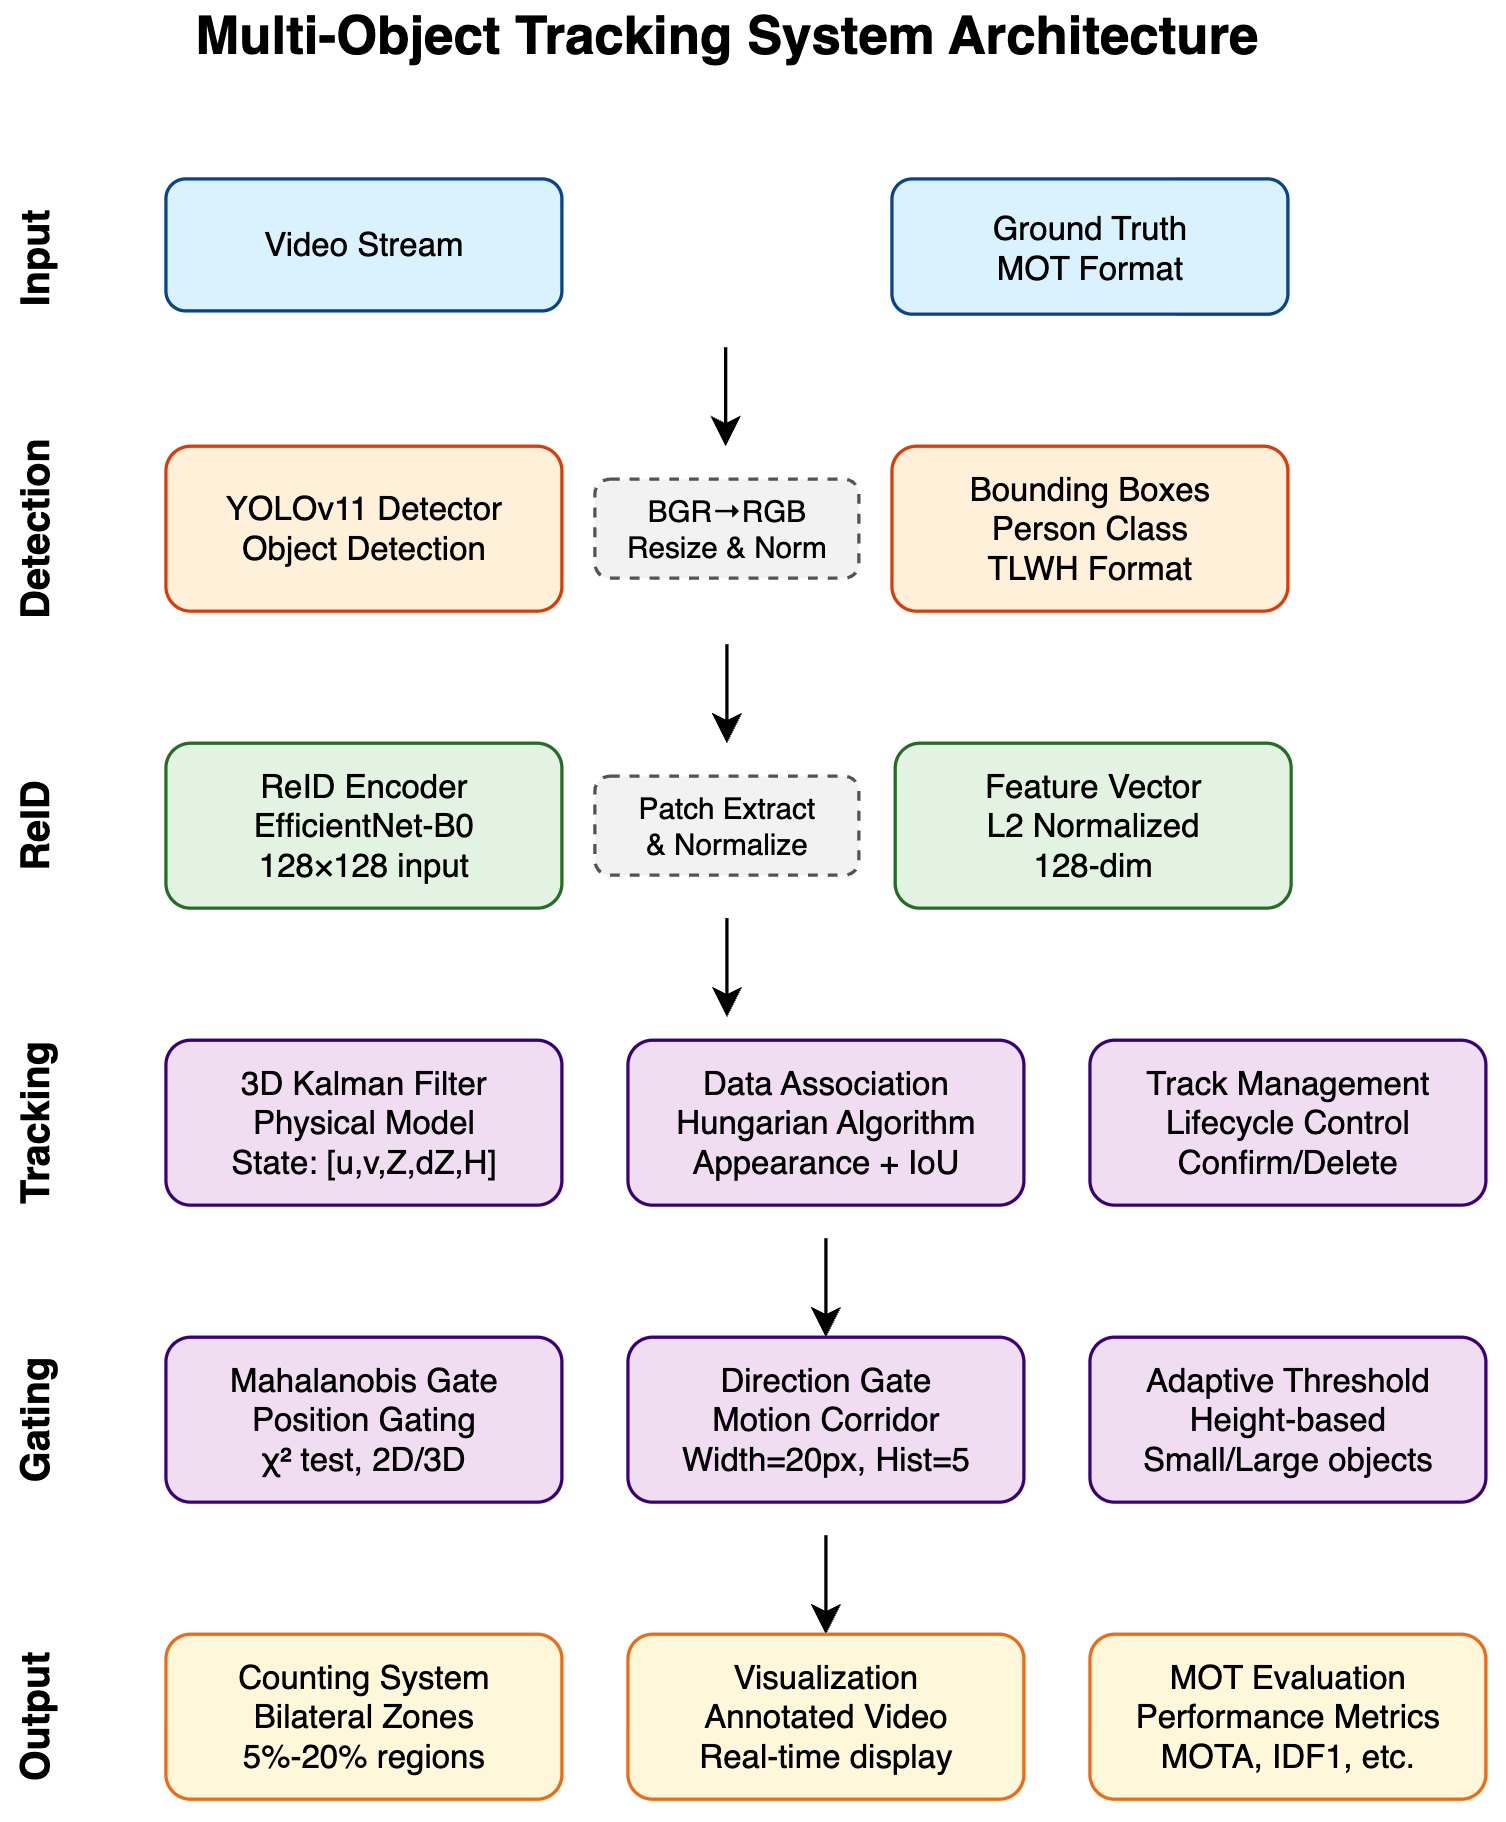
\includegraphics[width=0.8\textwidth]{pictures/OurMulti-ObjectTrackingSystemArchitecture.png}
\caption{Overall Multi-object Tracking System Architecture. The system integrates YOLOv11-based object detection, EfficientNet-B0 ReID feature extraction, and a 3D physical Kalman filter for robust pedestrian tracking. The pipeline consists of five modules: (1) Input, which includes video streams and ground-truth annotations in MOT format; (2) Detection, where YOLOv11 detects pedestrian bounding boxes (TLWH format); (3) ReID, which extracts 128-dimensional L2-normalized feature vectors using an EfficientNet-B0 encoder; (4) Tracking and Gating, which performs data association via a Hungarian algorithm combining appearance and IoU metrics, managed by a 3D Kalman filter with state variables ${[X,\ Y,\ Z,\ \dot{Z},\ \ddot{Z},\ H]}$ and multiple gating strategies including Mahalanobis distance, directional motion corridors, and adaptive thresholds; and (5) Output, which provides bilateral-zone counting, annotated visualization, and MOTChallenge performance evaluation (MOTA, IDF1, etc.). This modular architecture ensures accurate, stable, and interpretable tracking across video sequences.}
    \label{fig:OurMOTSystemArchitecture}
\end{figure}

\subsection{Scene and Imaging Model}
We model a forward-facing camera rigidly mounted near the train head, with the optical axis aligned with the track tangent. Pedestrians on the platform stand at lateral distance $X$ from the track centerline and have 3D vertical coordinate $Y$ (both approximately constant over time in the camera frame). Let $(u,v)$ be pixel coordinates with intrinsics $(f,c_x,c_y)$, where $f$ is the focal length (in pixels), $c_x$ is the principal point x-coordinate, and $c_y$ is the principal point y-coordinate. Denote by $Z(t)$ the depth coordinate along the track direction from camera to a target head. During arrival, motion is captured by
\begin{equation}
Z(t)=Z_0+\dot{Z}_0 t + \tfrac{1}{2}\ddot{Z}\,t^{2}, \quad \ddot{Z}<0.
\end{equation}
Under a pinhole model the projection obeys
\begin{equation}
u(t)=c_x+f\tfrac{X}{Z(t)},\quad v(t)=c_y+f\tfrac{Y}{Z(t)},\quad h_{\text{px}}(t)=f\tfrac{H(t)}{Z(t)},
\end{equation}
where $H(t)$ represents the physical head height above the platform surface, and $Z(t)$ is the depth coordinate in the camera coordinate system (with $Z_t$ pointing along the track towards the platform). This provides a stable mapping between apparent size and depth. This scene model underpins the Phys-6D tracker by explicitly coupling pixel height $h_{\text{px},t}$ and depth $Z_t$, and guides counting-band placement near image borders where perspective magnification and occlusions are prominent. Camera intrinsics used in experiments are reported with the calibration results in Chapter~5.

\textbf{Figure}~\ref{fig:3TrackingTrackGraph} illustrates the 2D planar trajectory visualization of human head bounding box centers from three video sequences, generated from MOT-format ground truth annotations. This visualization demonstrates the typical movement patterns and spatial distribution of pedestrian trajectories in our railway platform scenarios.

\begin{figure}[H]
    \centering
    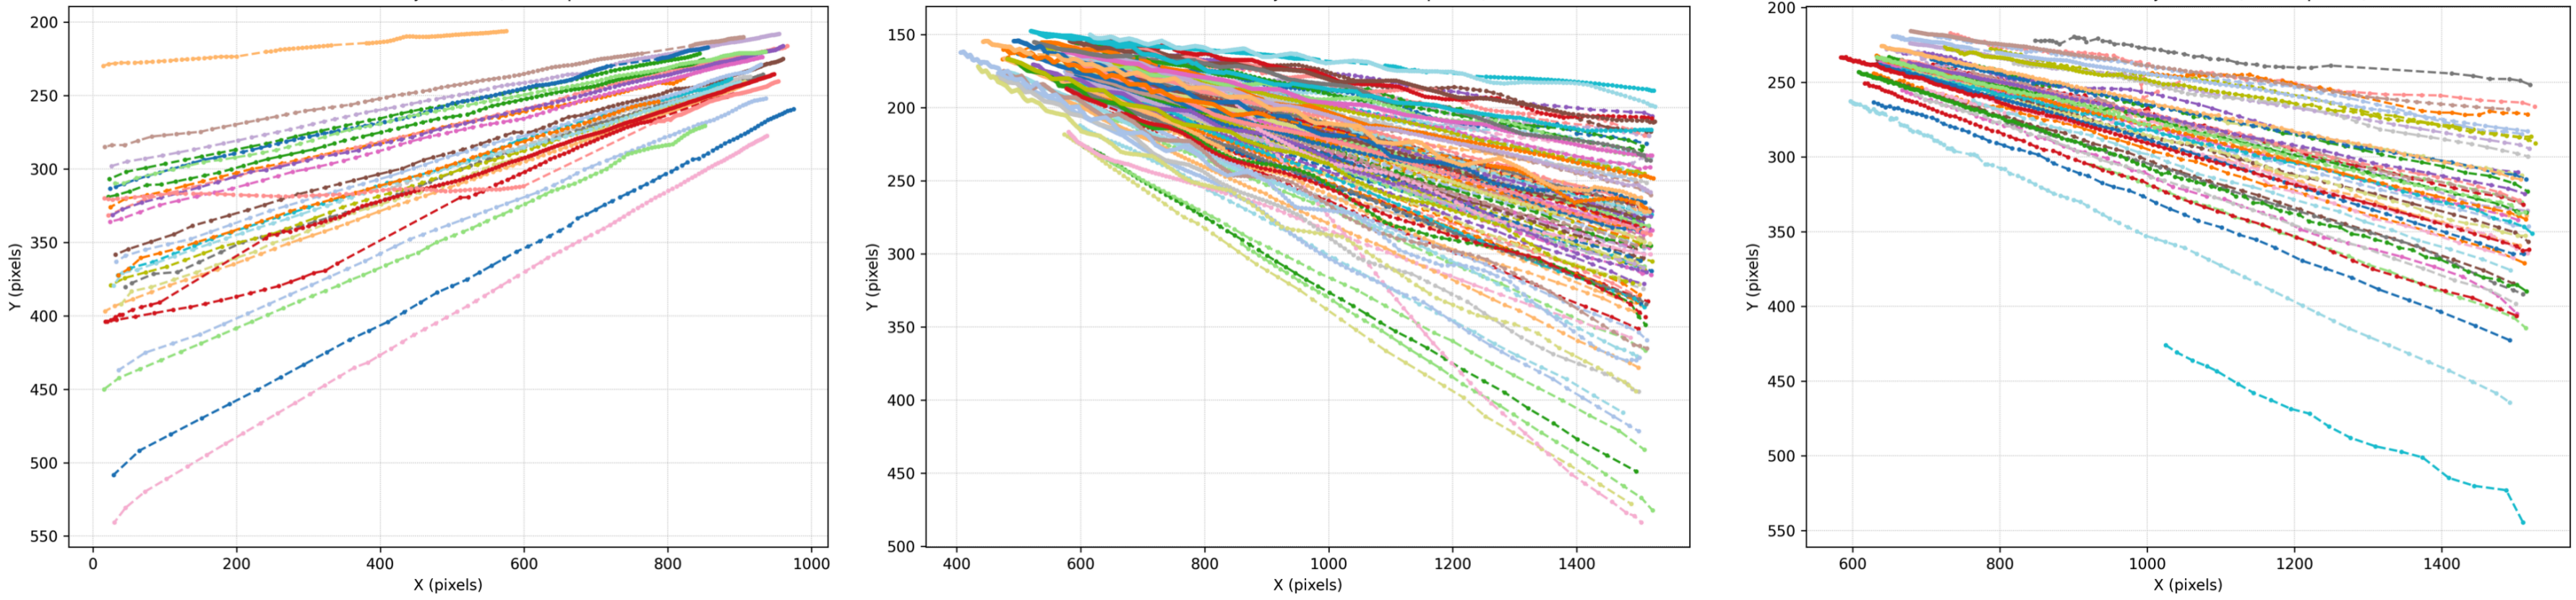
\includegraphics[width=0.95\textwidth]{pictures/3 Tracking Track Graph.png}
    \caption{2D planar trajectory visualization of human head bounding box centers from three video sequences, generated from MOT-format ground truth annotations.}
    \label{fig:3TrackingTrackGraph}
\end{figure}


\subsection{Implementation Details}
We provide complete implementation specifications for reproducibility:

\textbf{Detector Configuration:} YOLOv11m with two-stage transfer learning: (1) pre-train on CrowdHuman dataset; (2) fine-tune on railway/platform head images with the first 10 backbone layers frozen. Training uses SGD optimizer (lr=1e-2, weight decay=5e-4), cosine annealing scheduler, and mixed precision. Inference thresholds: confidence=0.5, IoU=0.7, input size=640×640.

\textbf{ReID Configuration:} EfficientNet-B0 backbone with input preprocessing: direct resizing to target size (128x128), horizontal flip augmentation, and color jitter. Training uses triplet loss with margin α=0.5, Adam optimizer (lr=1e-4), StepLR scheduler (step\_size=10, gamma=0.5).

\textbf{Tracking Configuration:} DeepSORT with three Kalman state-space configurations. Association uses linear combination of Mahalanobis distance (motion) and cosine distance (appearance) with weight λ=0.5. Cascaded matching prioritizes recently observed tracks. Gating thresholds: CV-8D uses standard DeepSORT thresholds; CA-12D uses stricter thresholds due to higher dimensionality;Phys-6D uses geometry-aware thresholds based on depth constraints.

\textbf{Counting Configuration:} Virtual counting bands with Start=0.05, End=0.20 (relative to image width), persistence threshold N=2 frames. Per-ID de-duplication and end-of-video compensation are applied. Final count uses maximum of left/right counts to avoid non-platform bias.

\textbf{System Integration:} All components run on GPU with real-time processing capability. The complete pipeline processes video frames sequentially: detection → ReID feature extraction → Kalman prediction → data association → track update → counting logic.

\subsection{YOLOv11 Model}

In our method, YOLOv11m is used specifically for head detection to reduce occlusion-induced misses on full bodies and to stabilize localization for small targets. We adopt transfer learning and fine-tuning to specialize for platform heads (details summarized below and results in Chapter~5), while retaining the architectural advantages of YOLOv11 for real-time deployment.

In 2015, Redmon et al. introduced the YOLO algorithm, a landmark in object detection \cite{76_redmon2016lookonceunifiedrealtime}. As its name suggests, YOLO detects objects and their locations in a single pass over the image by formulating detection as a regression problem, in contrast to traditional two-stage pipelines. As illustrated in \textbf{Fig.}~\ref{fig:yolosystem-cn} and \textbf{Fig.}~\ref{fig:yoloarchitecture-cn}, a single convolutional neural network (CNN) jointly predicts bounding boxes and class probabilities across the entire image \cite{77_Du_article}, simplifying the detection process compared to more complex traditional methods. Recent studies have demonstrated the computational efficiency advantages of YOLO-based approaches in edge computing scenarios, where single-stage detection models can reduce resource usage by nearly 50\% compared to multiple specialized networks \cite{s23136138}.
\begin{figure}[H]
    \centering
    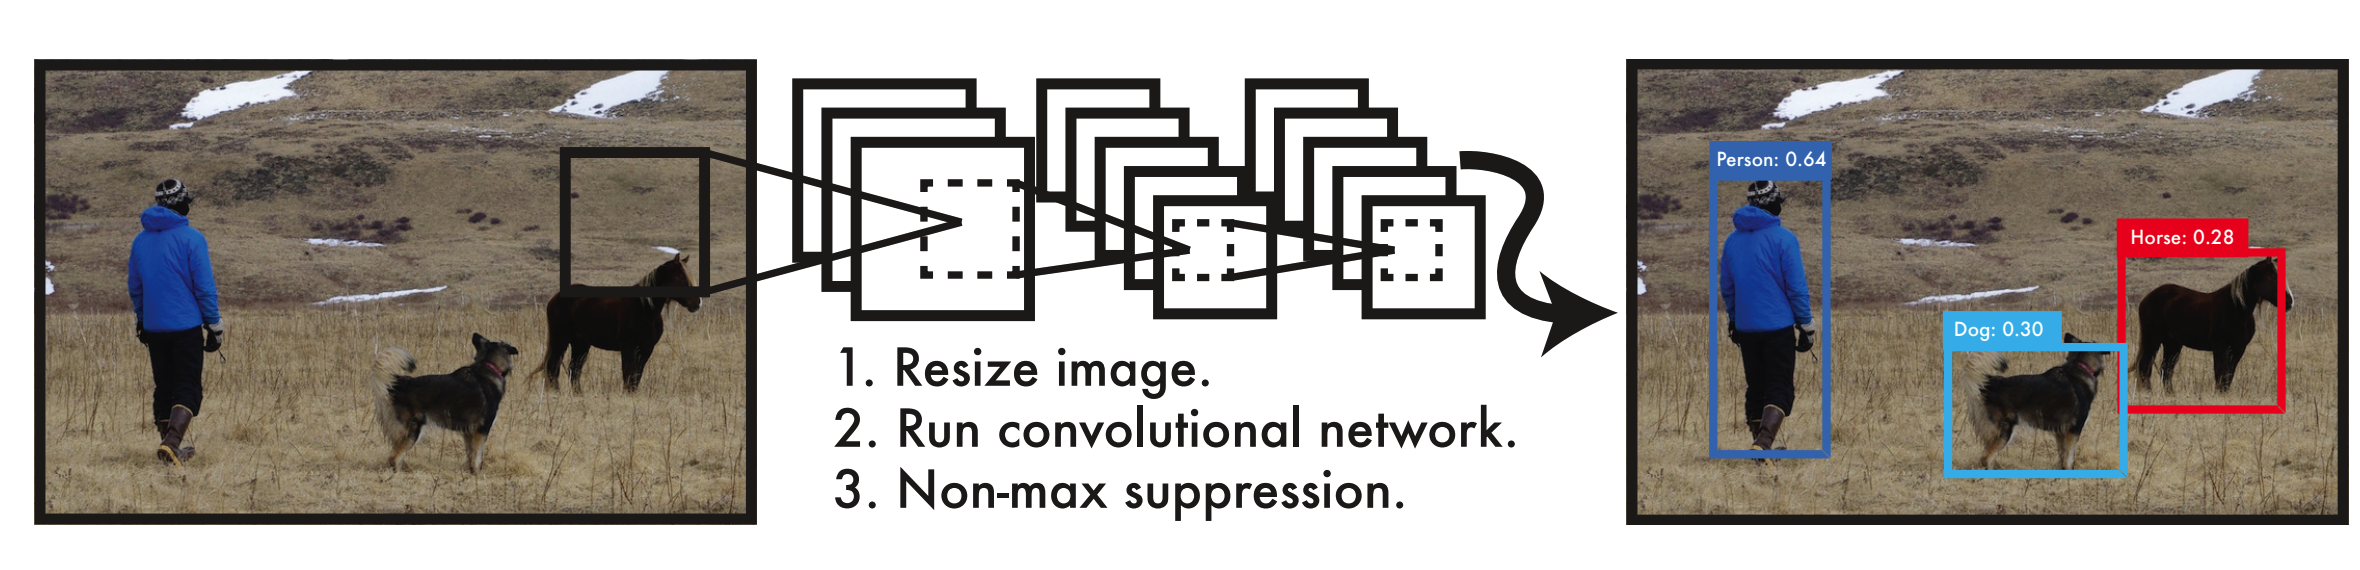
\includegraphics[width=0.8\textwidth]{pictures/The YOLO Detection System.png}
    \caption{YOLOv1 Detection System \cite{76_redmon2016lookonceunifiedrealtime}}
    \label{fig:yolosystem-cn}
\end{figure}
\begin{figure}[H]
    \centering
    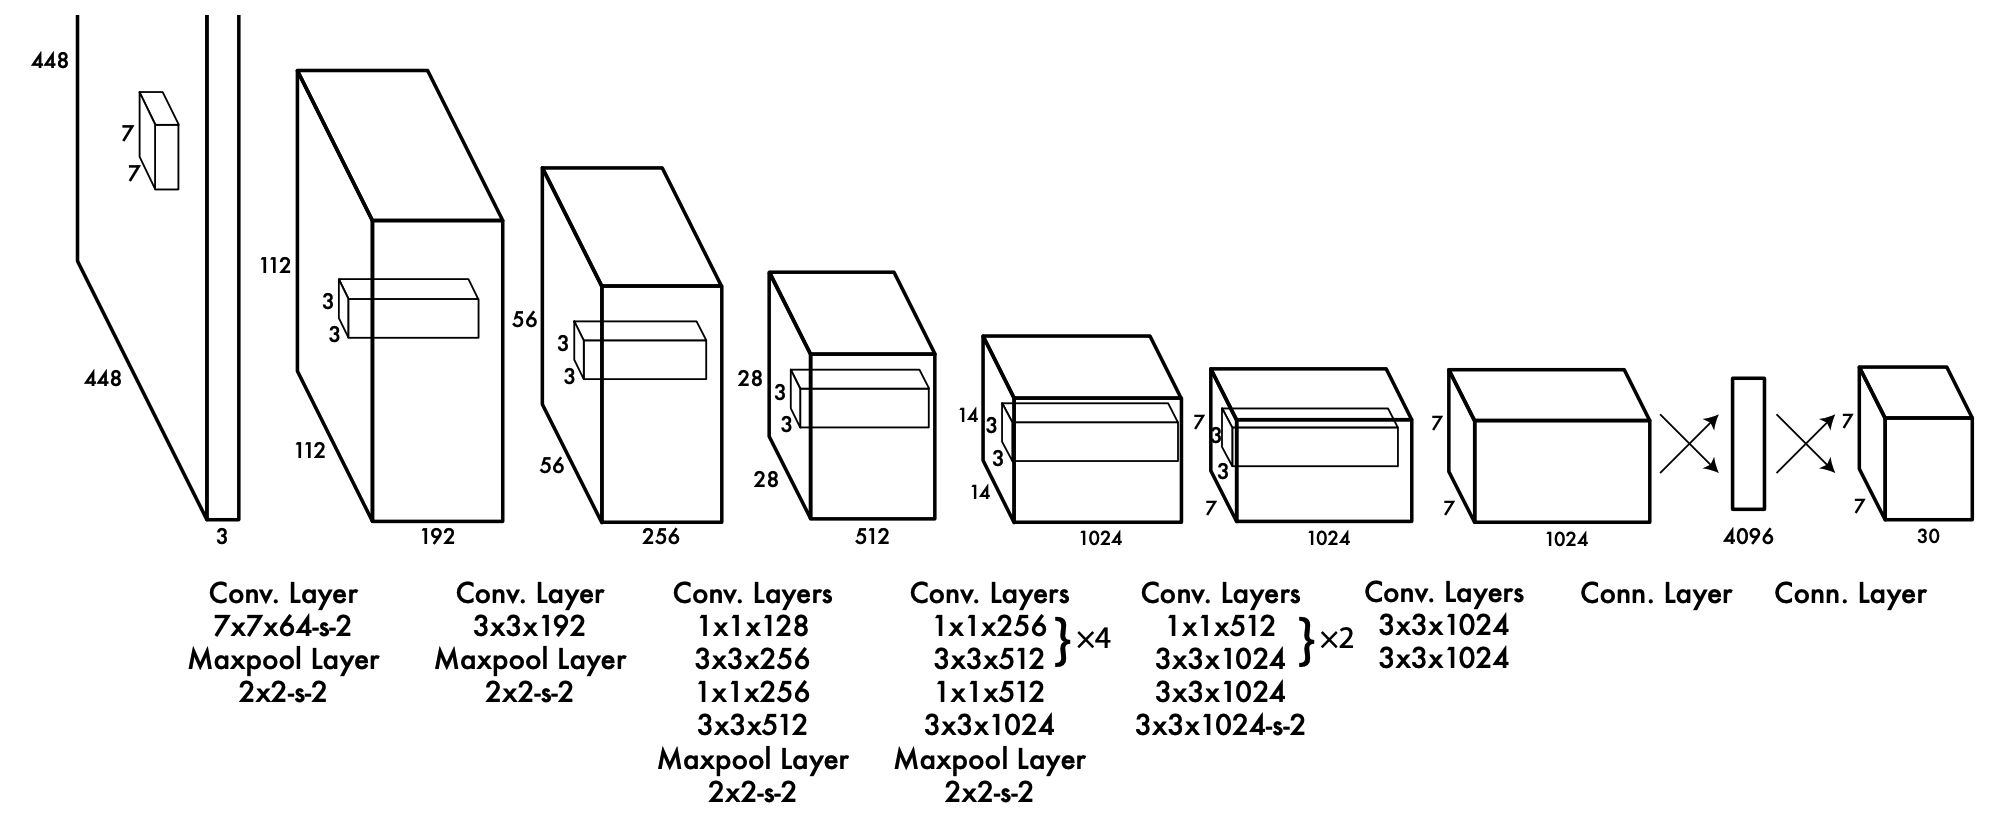
\includegraphics[width=0.8\textwidth]{pictures/The YOLO Architecture.png}
    \caption{YOLOv1 Architecture \cite{76_redmon2016lookonceunifiedrealtime}}
    \label{fig:yoloarchitecture-cn}
\end{figure}

YOLOv11 represents a significant step forward in the YOLO family, announced at the YOLOVision 2024 (YV24) conference. It refines network design and training strategies to further improve detection accuracy and speed \cite{74_yolo11_Jocher_Ultralytics_YOLO_2023}. As noted in Related Work, using full-body cues for detection degrades substantially in crowded scenes due to heavy occlusions, whereas head cues are more discriminative and less occluded yet remain underexplored. In high-density settings, frequent and severe occlusions hinder full-body recognition, while heads, being at the upper body and less occluded with more stable shape cues, are easier to localize. Head sizes also vary less with pose, reducing both false positives and false negatives. Accordingly, we detect heads with YOLOv11 as the basis for counting.

As shown in \textbf{Fig.}~\ref{fig:benchmarkingyolo11}, YOLOv11 introduces notable architectural and training enhancements that push the boundary of accuracy, speed, and efficiency \cite{75_khanam2024yolov11overviewkeyarchitectural}.
\begin{figure}[H]
    \centering
    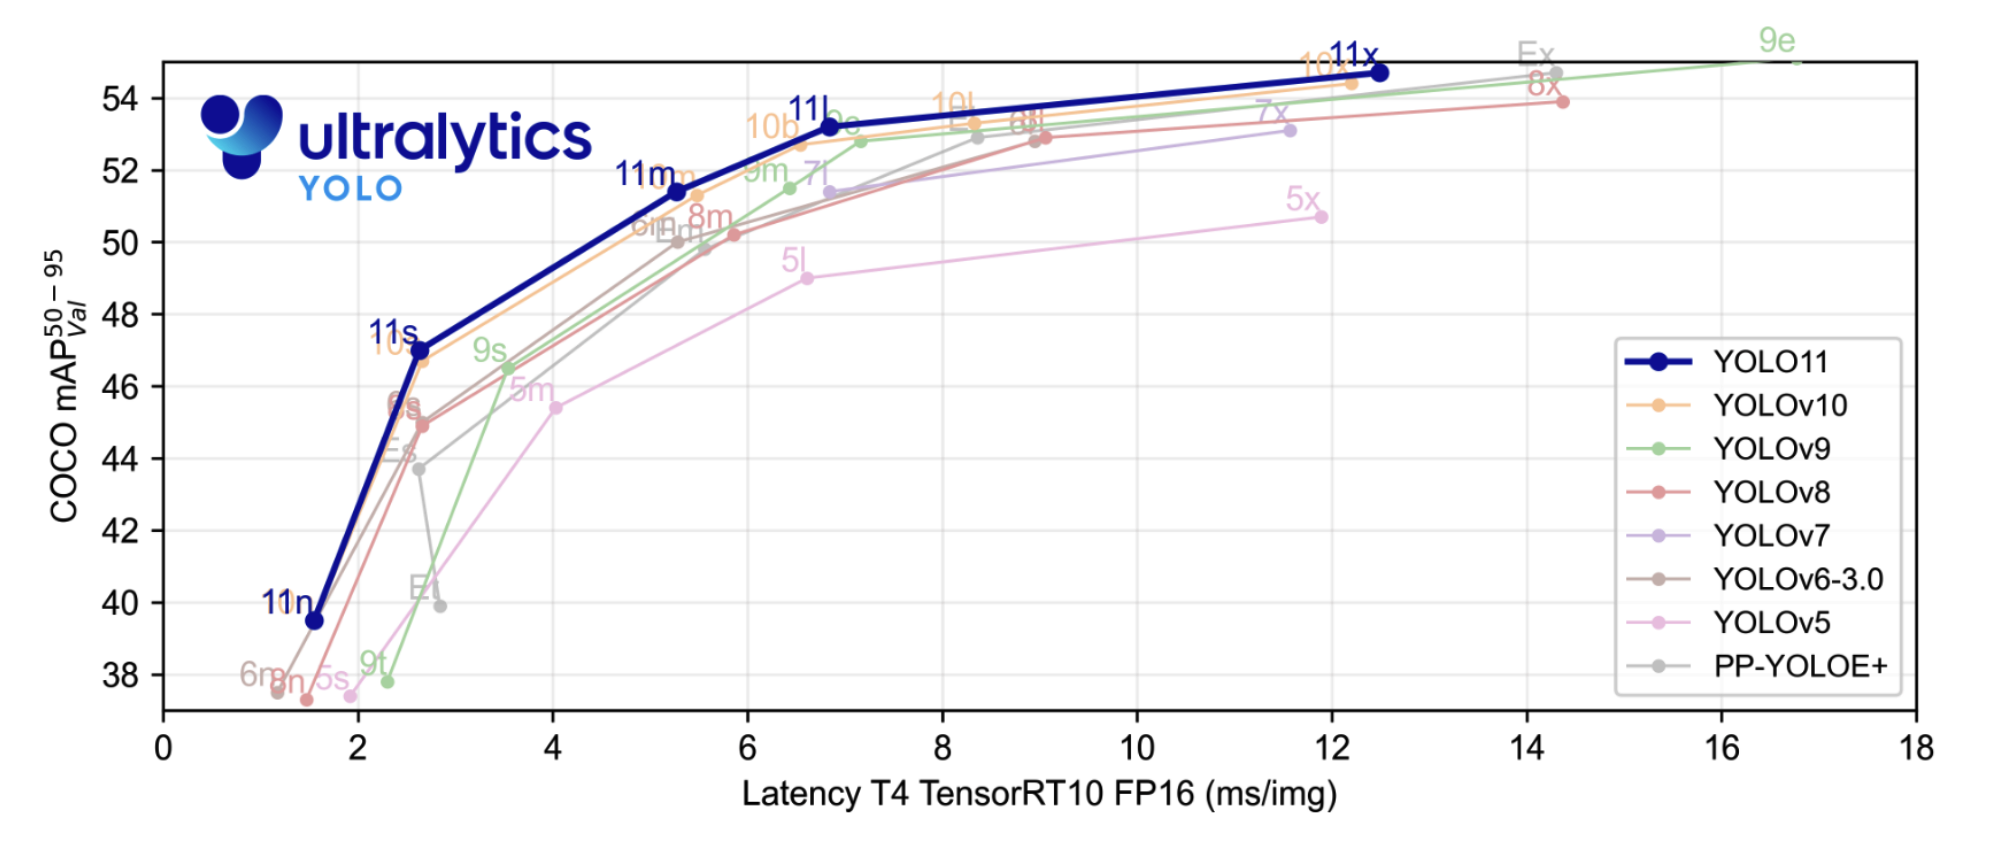
\includegraphics[width=0.6\textwidth]{pictures/BenchmarkingYOLOv11AgainstPrevious Versions.png}
    \caption{Benchmarking YOLOv11 Against Previous Versions\cite{74_yolo11_Jocher_Ultralytics_YOLO_2023}}
    \label{fig:benchmarkingyolo11}
\end{figure}




\subsection{Key Architectural Components of YOLOv11}
The YOLOv11 architecture comprises three fundamental components (\textbf{Fig.}~\ref{fig:yolo11architecture-cn}). First, the backbone serves as the primary feature extractor, transforming raw images into multi-scale feature maps via CNNs. Second, the neck acts as an intermediate aggregation stage, enhancing and fusing features across scales. Third, the head produces the final predictions for localization and classification \cite{75_khanam2024yolov11overviewkeyarchitectural}.

\begin{figure}[H]
    \centering
    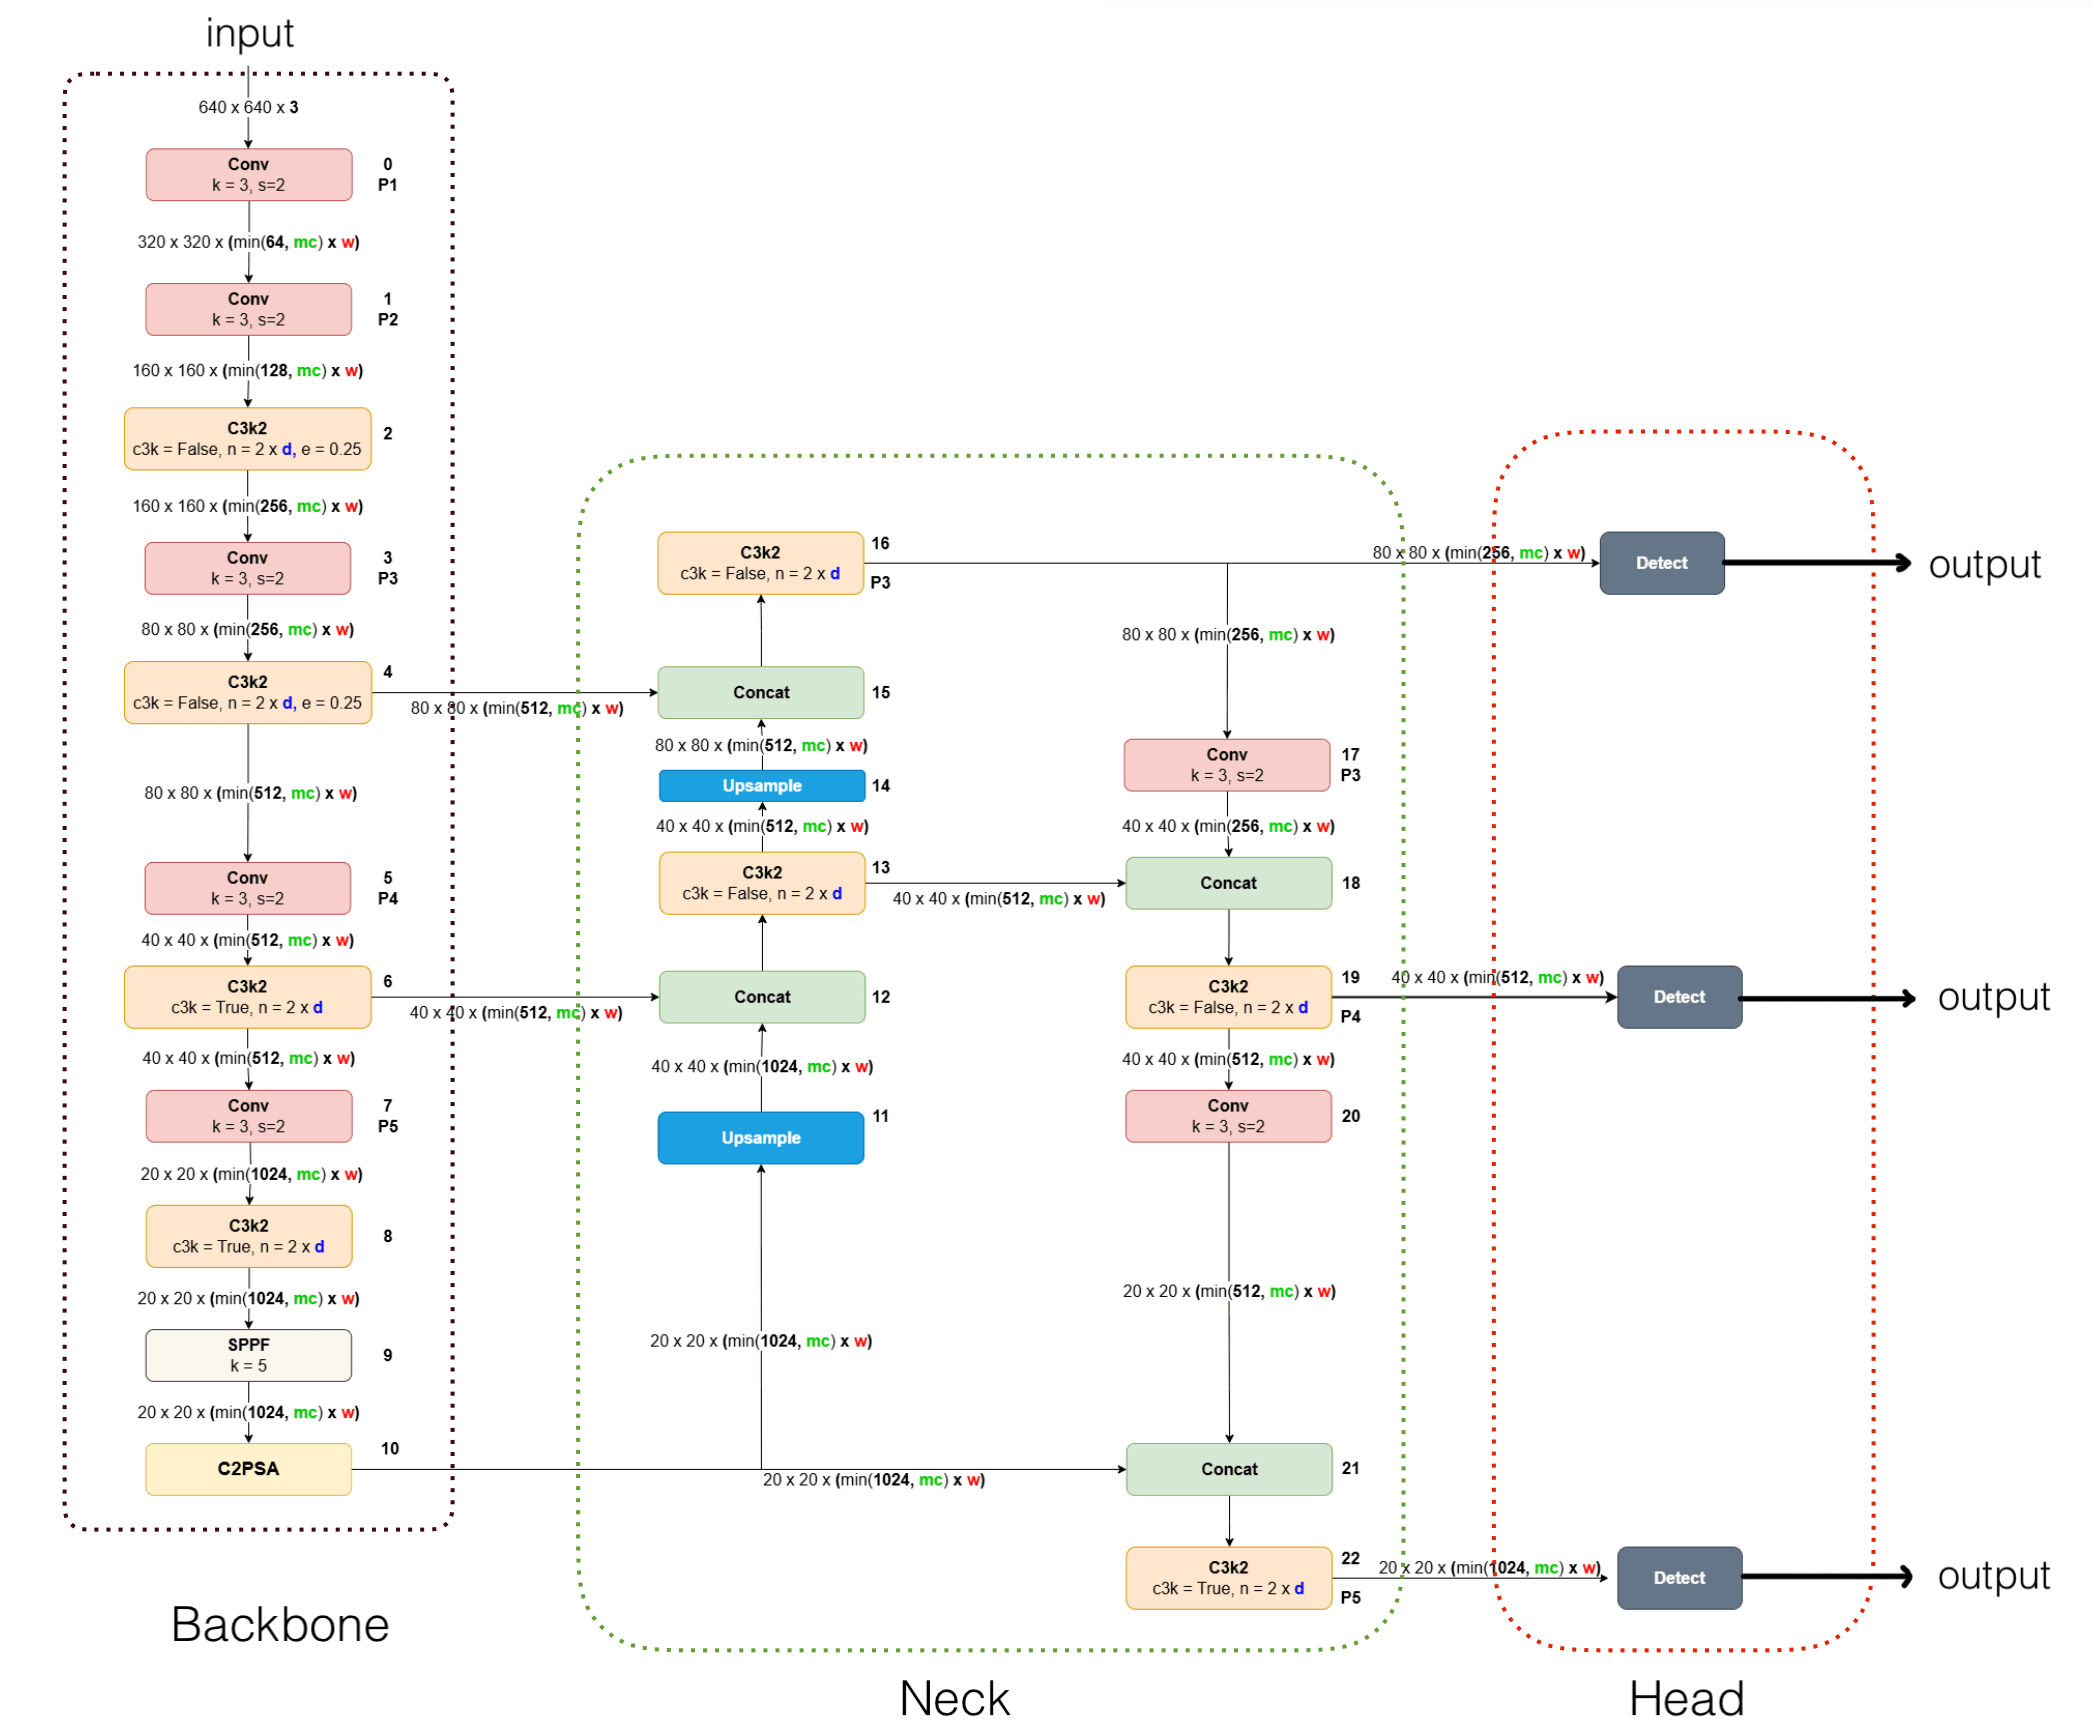
\includegraphics[width=0.92\textwidth]{pictures/Yolo11architecture.png}
    \caption{YOLOv11 Architecture\cite{80_ghosh_yolo11_2024}}
    \label{fig:yolo11architecture-cn}
\end{figure}

YOLOv11 introduces significant architectural and training enhancements that push the boundaries of accuracy, speed and efficiency. As shown in \textbf{Fig.}~\ref{fig:Keyarchite-cn}, the key architectural components of YOLOv11 are illustrated.
\begin{figure}[H]
    \centering
    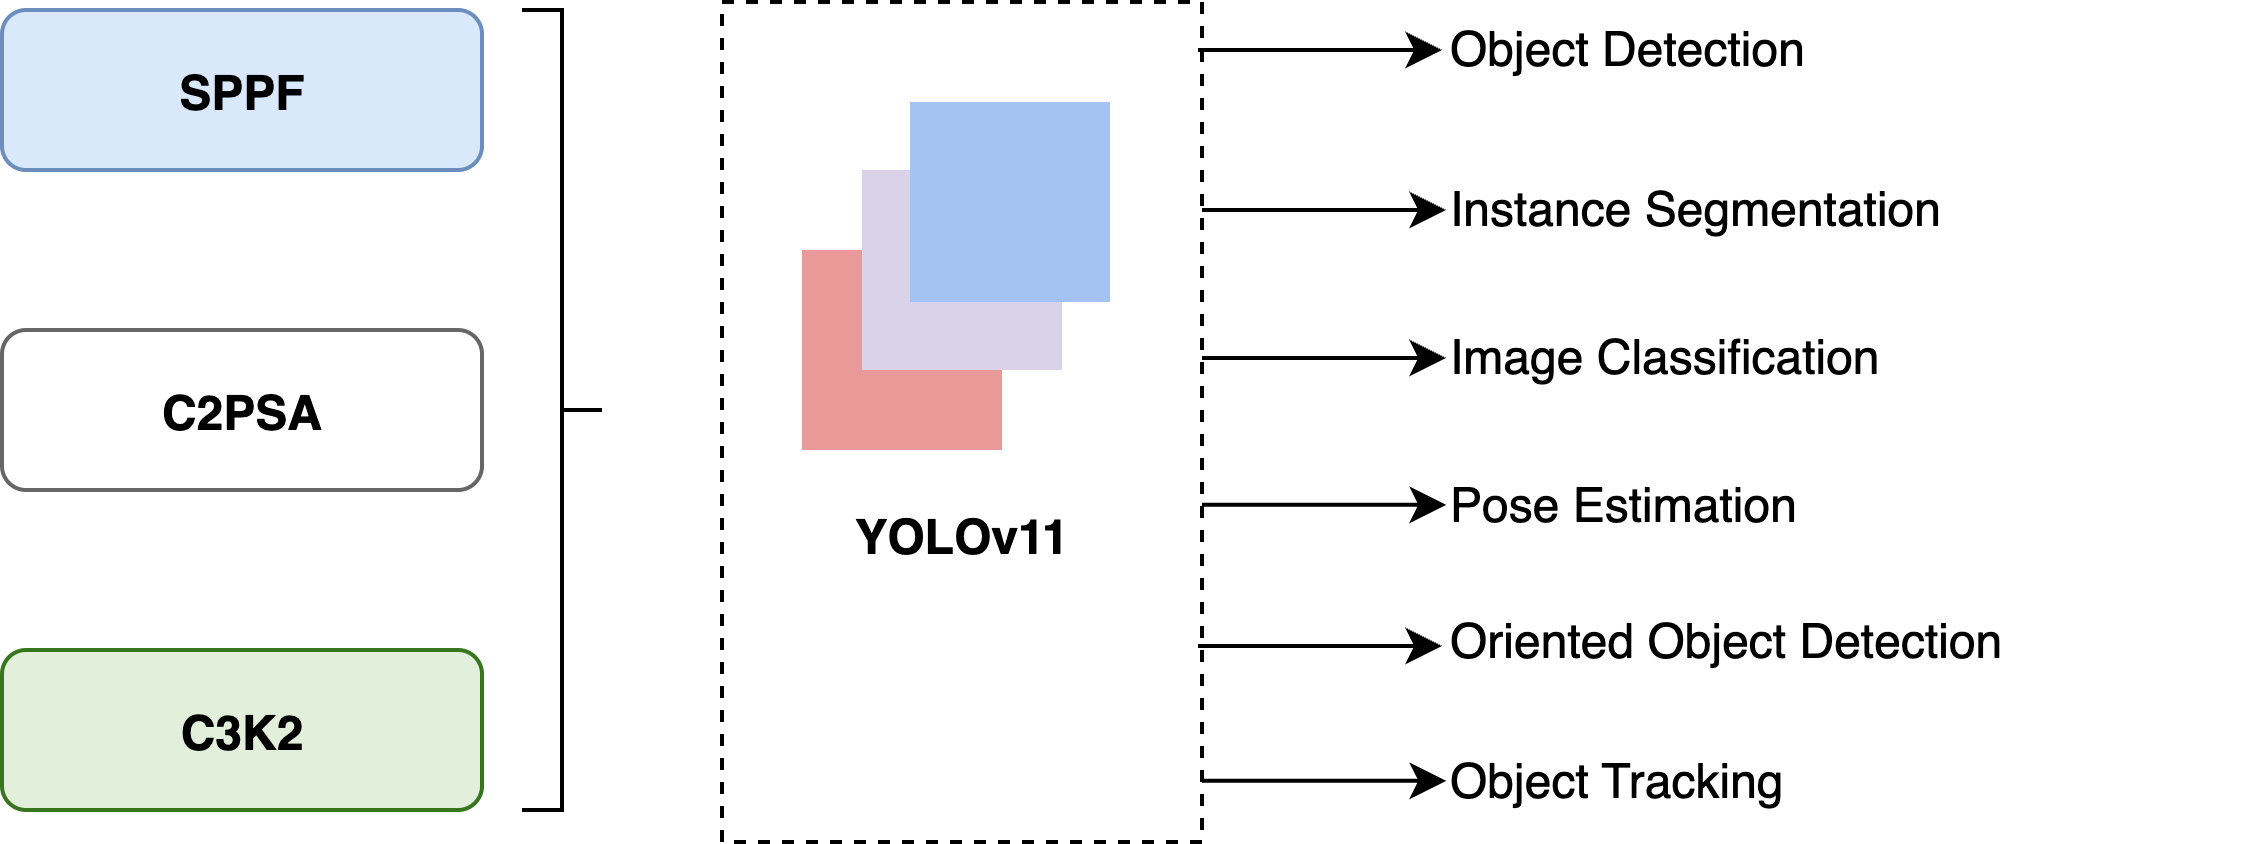
\includegraphics[width=0.7\linewidth]{pictures/key architectural modules in YOLO11.png}
    \caption{Key Architectural Modules in YOLOv11 \cite{80_ghosh_yolo11_2024}}
    \label{fig:Keyarchite-cn}
\end{figure}

\subsubsection{Backbone Network}
The backbone extracts features at multiple scales by stacking convolutional layers and specialized blocks to produce feature maps at varying resolutions. Initial convolutional layers downsample the input, progressively reducing spatial dimensions while increasing channel depth.

\paragraph{SPPF and C2PSA}
YOLOv11 retains the Spatial Pyramid Pooling - Fast (SPPF) block and introduces the Cross Stage Partial with Spatial Attention (C2PSA) block \cite{80_ghosh_yolo11_2024}. As shown in \textbf{Fig.}~\ref{fig:C2PSA-cn}, C2PSA enhances spatial attention, enabling the model to focus more effectively on salient regions. By pooling spatial features, C2PSA strengthens localization of objects at different sizes and positions.
\begin{figure}[H]
    \centering
    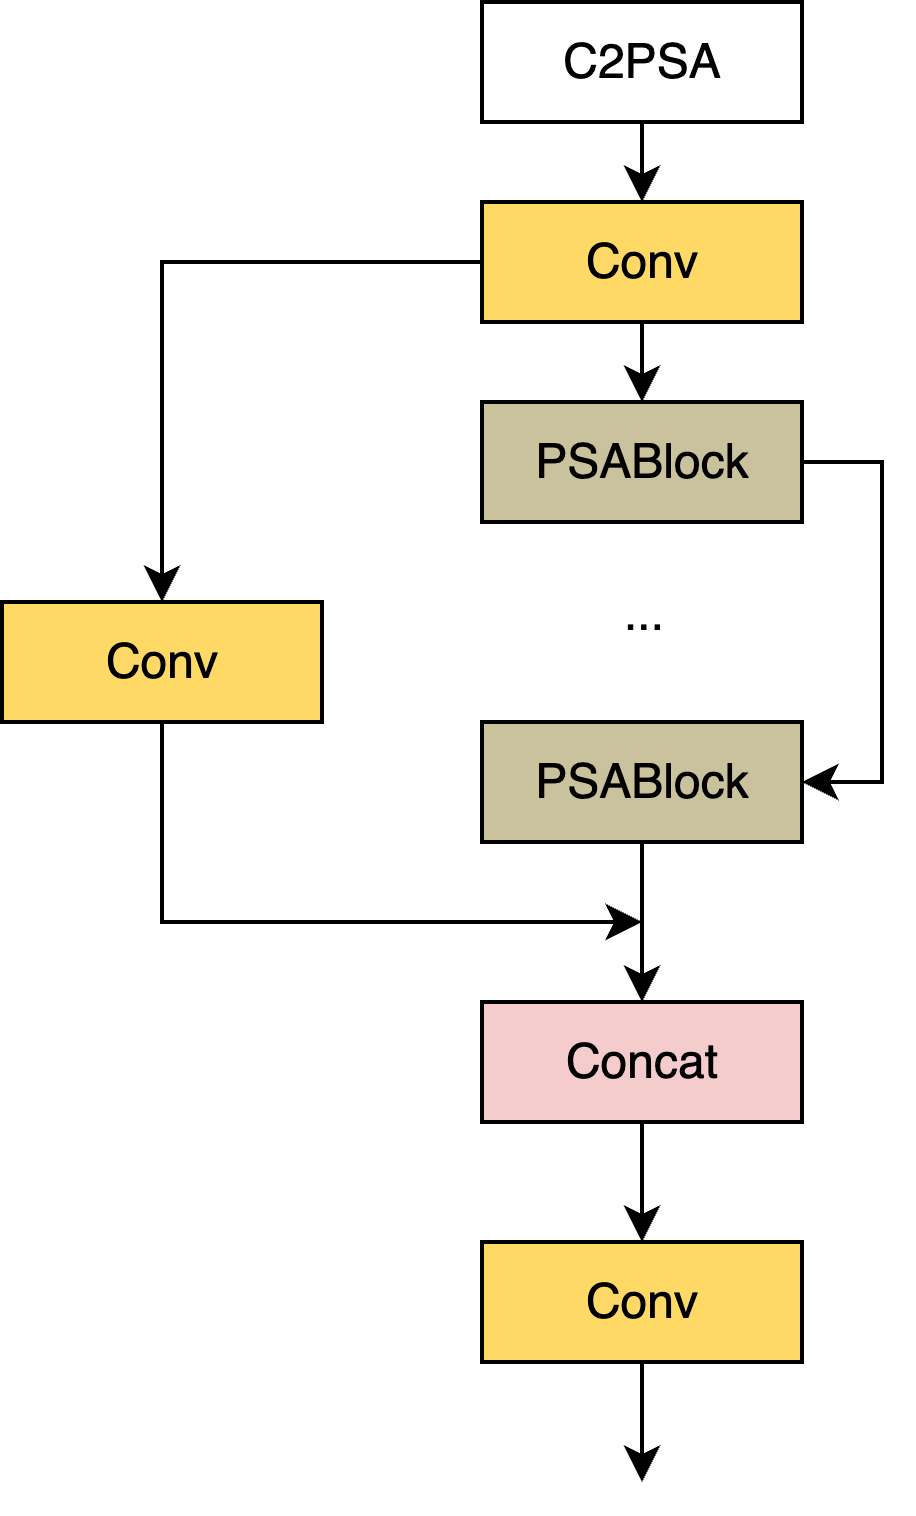
\includegraphics[width=0.25\linewidth]{pictures/C2PSA.png}
    \caption{YOLOv11 C2PSA Module \cite{80_ghosh_yolo11_2024}}
    \label{fig:C2PSA-cn}
\end{figure}

\subsubsection{Neck Network}
The neck bridges backbone and head, aggregating features from multiple scales for downstream prediction.

\paragraph{C3K2 block}
YOLOv11 replaces the neck's C2f blocks with C3k2 blocks, a more computationally efficient variant of the CSP (Cross Stage Partial) bottleneck. As shown in \textbf{Fig.}~\ref{fig:C3K2-cn}, it uses two smaller convolutions instead of a single large convolution (as in YOLOv8 \cite{81_noauthor_what_2024}). The "k2" indicates smaller kernel sizes, improving speed while maintaining performance \cite{75_khanam2024yolov11overviewkeyarchitectural}.
\begin{figure}[H]
    \centering
    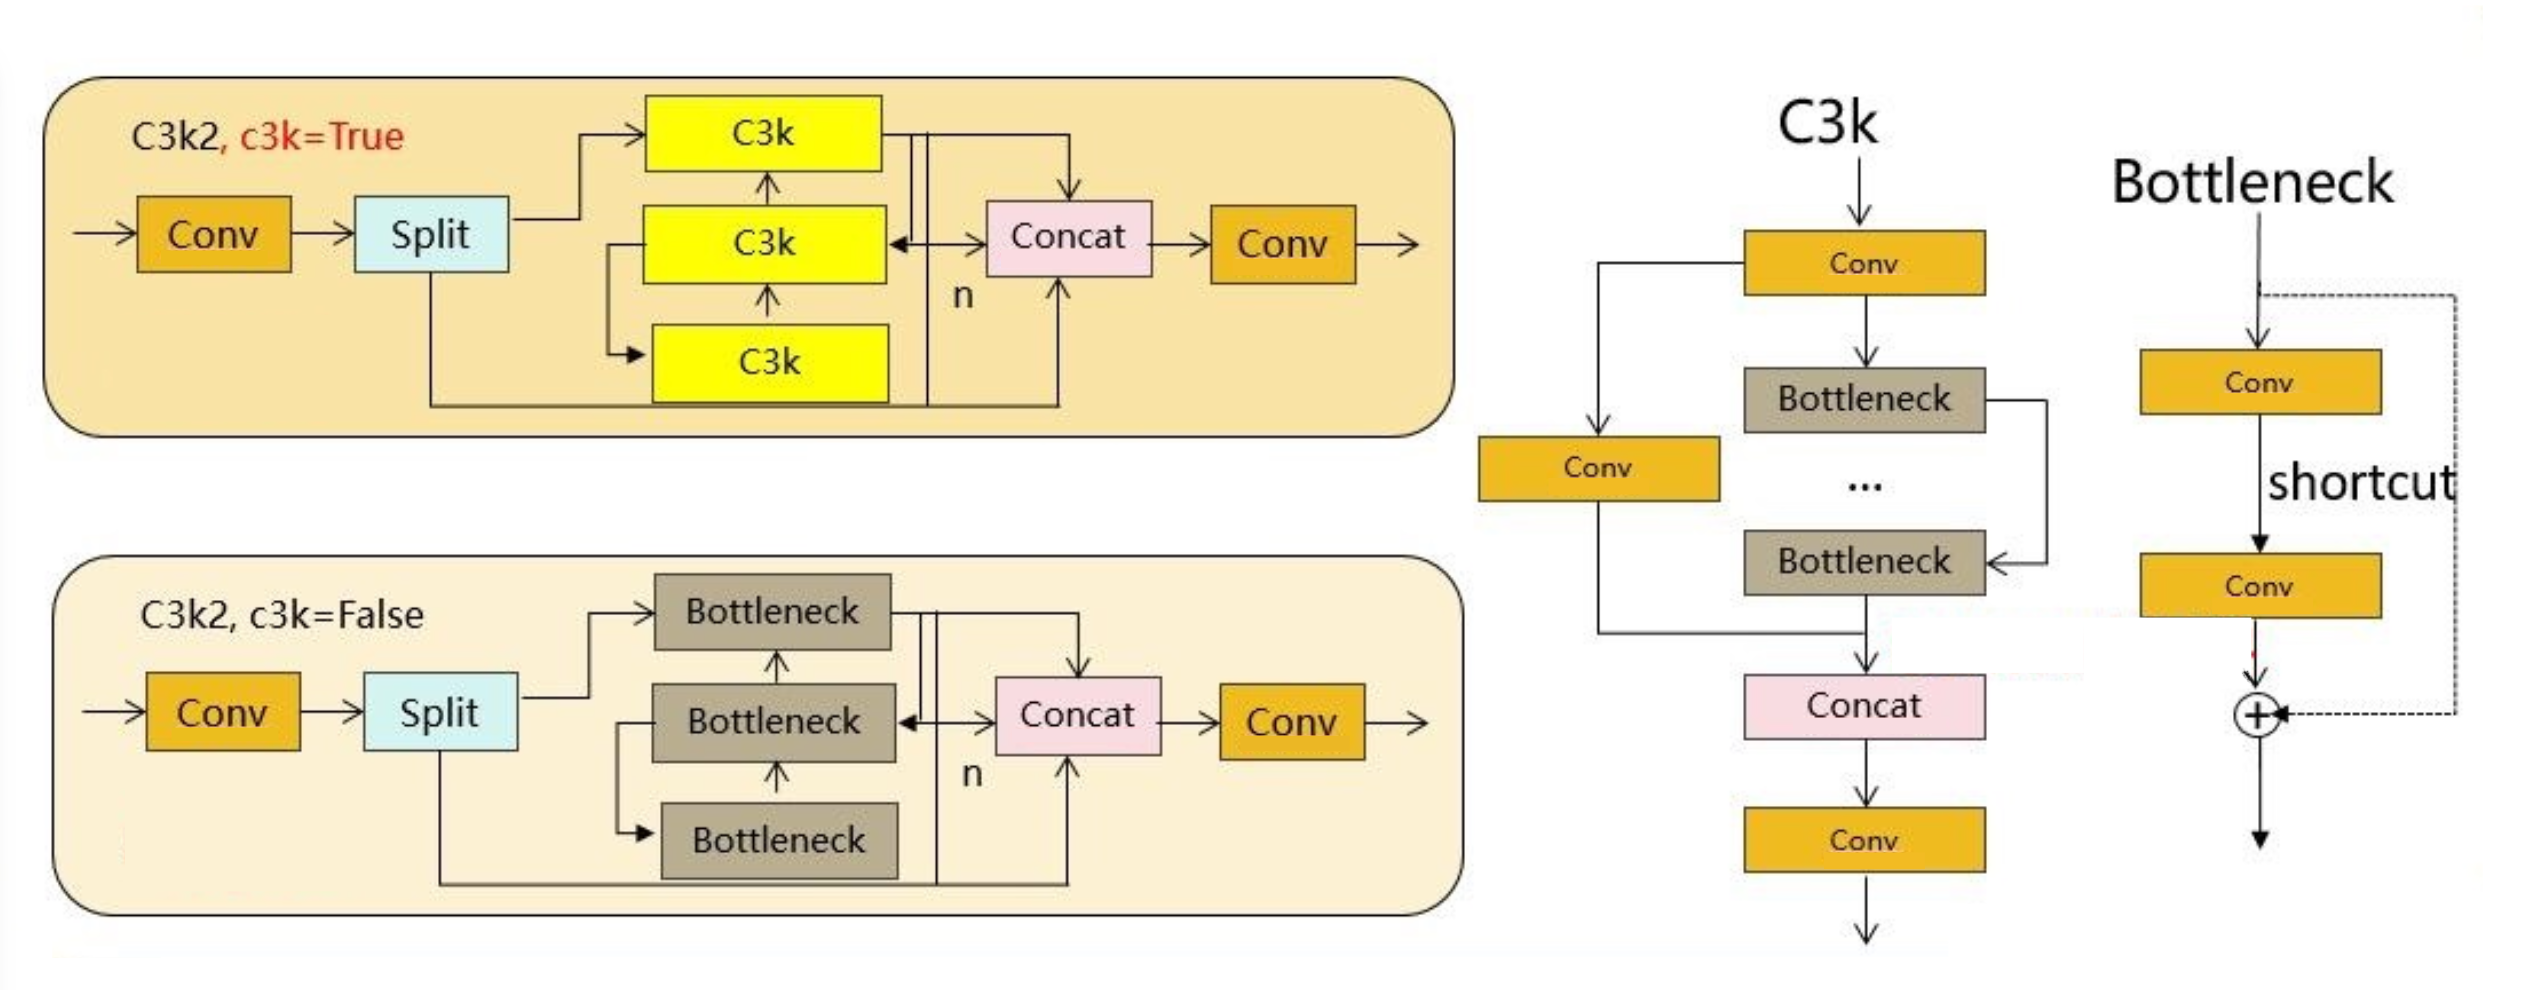
\includegraphics[width=0.8\linewidth]{pictures/C3K2.png}
    \caption{C3K2 Module\cite{83_ultralytics_yolo11_2025}}
    \label{fig:C3K2-cn}
\end{figure}

Attention mechanism
An important addition in YOLOv11 is increased emphasis on spatial attention via C2PSA. This mechanism helps focus on key regions, yielding more accurate detection of small or partially occluded objects. This distinguishes YOLOv11 from YOLOv8, which lacks this specific attention module \cite{80_ghosh_yolo11_2024,75_khanam2024yolov11overviewkeyarchitectural}.

\subsubsection{Detection Head}
The head performs multi-scale predictions, outputting bounding-box parameters (center, width, height), class probabilities, and objectness scores. The input image is partitioned into grid cells, each responsible for objects whose centers fall within it.

\paragraph{C3k2 blocks}
YOLOv11 employs multiple C3k2 blocks within the head to process and refine features across different depths. Behavior varies with the parameter c3k:\\
    • If c3k = False, C3k2 behaves similarly to C2f with a standard bottleneck.\\
    • If c3k = True, the bottleneck is replaced with a C3 module for deeper, more expressive feature extraction.\\
Key properties of C3k2:\\
    • Faster processing via two smaller convolutions instead of a single large convolution.\\
    • Parameter efficiency as a more compact CSP bottleneck.\\
Additionally, the C3k module allows customizable kernel sizes for improved flexibility.

\paragraph{CBS blocks}
After C3k2 blocks, YOLOv11's head includes several CBS (Convolution–BatchNorm–SiLU) layers \cite{81_noauthor_what_2024}, which further refine features by extracting salient cues, stabilizing flow via batch normalization, and introducing nonlinearity through SiLU.

\paragraph{Final convolution and detection layers}  
Each detection branch ends with Conv2D layers that reduce features to the required outputs for bounding-box regression and classification. The final detection layer aggregates predictions:\\
    • Bounding-box coordinates for localization.\\  
    • Objectness scores.\\  
    • Class probabilities.\\

\subsection{DeepSORT}
We next introduce the DeepSORT multi-object tracker as used in our method. Our implementation extends the standard DeepSORT framework with several key modifications: (1) we replace the original CNN-based appearance extractor with EfficientNet-B0 for improved feature quality; (2) we introduce three different Kalman state-space configurations (CV-8D, CA-12D, and Phys-6D) instead of the standard constant-velocity model; and (3) we adapt the association thresholds and parameters for railway platform scenarios. Our tracker fuses appearance (EfficientNet-B0 embeddings) and motion (Kalman state-space models) with cascaded association to preserve identities under occlusions. Recent advances in multi-object tracking have demonstrated the effectiveness of combining local and global pose estimation for precise tracking of similar objects, particularly in scenarios with geometric ambiguities and occlusions \cite{pose_estimation_2022}. DeepSORT\cite{211}, an extension of SORT\cite{220}, combines deep appearance embeddings with motion information. The pipeline (\textbf{Fig.}~\ref{fig:DeepSORT-cn}) comprises deep appearance feature extraction, a Kalman filter, and data association.
\begin{figure}[H]
    \centering
    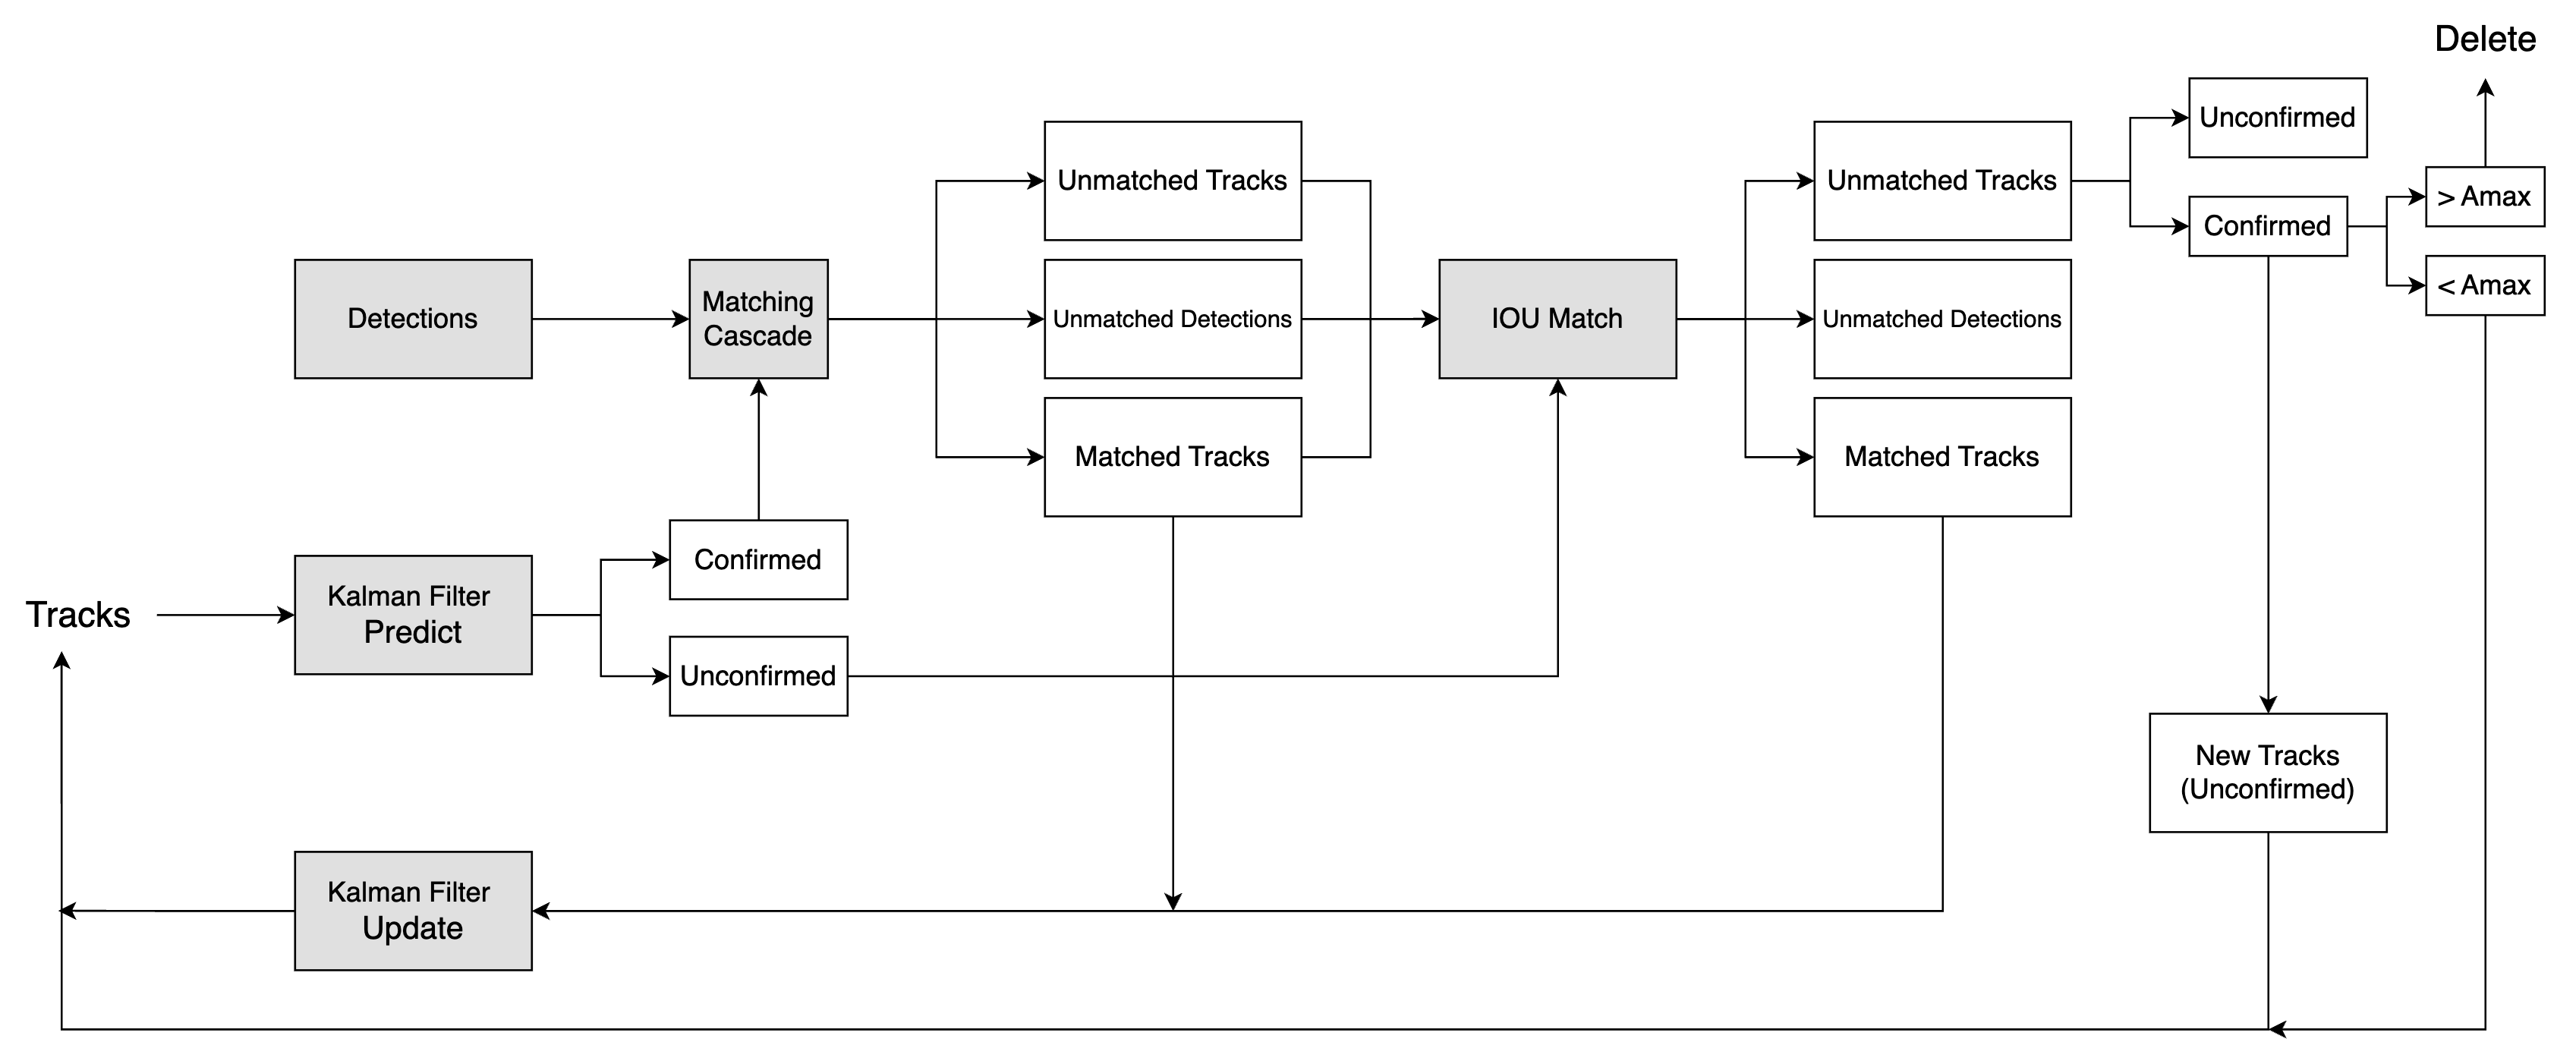
\includegraphics[width=0.99\textwidth]{pictures/DeepSORTAlgorithmStructure.png}
    \caption{DeepSORT architecture\cite{212}. The workflow can be summarized as follows:
    (1) Object detection: a high-performance detector identifies targets in each frame and outputs bounding boxes with confidences \cite{174}.
    (2) Motion prediction: a Kalman filter predicts current positions and motion states for existing tracks \cite{174}.
    (3) Feature extraction: deep appearance embeddings are computed for detections via a ReID model \cite{179}.
    (4) Data association: detections are matched to predicted tracks using a cost that combines motion (Mahalanobis distance) and appearance (cosine distance), solved with the Hungarian algorithm; a cascaded strategy further improves matching \cite{104}.
    (5) Track update and management: matched tracks are updated; unmatched detections initialize new tracks; long-unmatched tracks are terminated.}
    \label{fig:DeepSORT-cn}
\end{figure}



\subsection{DeepSORT Core Modules}

\subsubsection{Object Detector}
In our system, tracking performance depends critically on the head detector; we adopt YOLOv11m as detailed above. For completeness, typical detectors include:\\
• YOLO family: widely adopted for its real-time performance and accuracy (e.g., YOLOv5/YOLOv7), and in our case YOLOv11.\\
• Faster R-CNN: representative two-stage detector used in early variants.\\
• SSD: one-stage detector also used in DeepSORT systems.\\
• CenterNet: an anchor-free detector that can jointly output boxes and identity embeddings.\\
Detector improvements (e.g., lightweight backbones, dilated convolutions, SPP) are often tailored to the application.

\subsubsection{Motion Model and Kalman Filter}
Kalman filtering estimates target motion states via iterative prediction and update. The classic DeepSORT state vector is an 8-dimensional vector $\mathbf{x} = [x, y, a, h, \dot{x}, \dot{y}, \dot{a}, \dot{h}]^T$ with $(x,y)$ the center, $a$ the aspect ratio, $h$ the height, and dots denoting velocities. Prediction and update follow standard linear dynamical systems formulas:
\begin{align*}
    \mathbf{x}_t &= \mathbf{F}\mathbf{x}_{t-1} + \mathbf{w}_t\\
    \mathbf{P}_t &= \mathbf{F}\mathbf{P}_{t-1}\mathbf{F}^T + \mathbf{Q}_t\\
    \mathbf{K}_t &= \mathbf{P}_t\mathbf{H}^T (\mathbf{H}\mathbf{P}_t\mathbf{H}^T + \mathbf{R})^{-1}\\
    \mathbf{x}_t &\leftarrow \mathbf{x}_t + \mathbf{K}_t (\mathbf{z}_t - \mathbf{H}\mathbf{x}_t)\\
    \mathbf{P}_t &\leftarrow (\mathbf{I} - \mathbf{K}_t\mathbf{H})\mathbf{P}_t
\end{align*}
where $\mathbf{F}$ is the state transition matrix, $\mathbf{H}$ is the observation matrix, $\mathbf{Q}_t$ is the process noise covariance, $\mathbf{R}$ is the measurement noise covariance, and $\mathbf{K}_t$ is the Kalman gain. While effective, a constant-velocity model can be inaccurate under strong acceleration or camera motion; extensions such as constant-acceleration models and adaptive noise can better handle nonlinearities. In our experiments, we instantiate three Kalman state-space (kinematic) configurations under DeepSORT and compare them in Chapter~5.

\subsection{Kalman State-Space Model Configurations}
We evaluate and deploy three Kalman state-space configurations under identical detector/ReID/association settings. Each model represents a different approach to motion modeling, from pure kinematics to physics-constrained estimation.

\subsubsection{CV-8D: Constant-Velocity Baseline Model}
The CV-8D model serves as our baseline, implementing the standard DeepSORT constant-velocity assumption with 8D state vector $[x, y, a, h, \dot{x}, \dot{y}, \dot{a}, \dot{h}]^T$ and measurement $[x, y, a, h]^T$, where $(x,y)$ denotes the bounding box center in image coordinates, $a$ is the aspect ratio, $h$ is the height, and dots denote velocities.

\textbf{State vector:}
\begin{equation}
\mathbf{x}_t = [x_t, y_t, a_t, h_t, \dot{x}_t, \dot{y}_t, \dot{a}_t, \dot{h}_t]^T \in \mathbb{R}^{8}
\end{equation}

\textbf{State transition matrix:}
\begin{equation}
\mathbf{F} = \begin{bmatrix}
\mathbf{I}_4 & \Delta t \cdot \mathbf{I}_4 \\
\mathbf{0}_{4 \times 4} & \mathbf{I}_4
\end{bmatrix}_{8 \times 8}
\end{equation}
where $\Delta t = 1$ frame (normalized time step), leading to:
\begin{equation}
\begin{bmatrix}
x_{t+1} \\ y_{t+1} \\ a_{t+1} \\ h_{t+1} \\ \dot{x}_{t+1} \\ \dot{y}_{t+1} \\ \dot{a}_{t+1} \\ \dot{h}_{t+1}
\end{bmatrix}
=
\begin{bmatrix}
x_t + \dot{x}_t \Delta t \\
y_t + \dot{y}_t \Delta t \\
a_t + \dot{a}_t \Delta t \\
h_t + \dot{h}_t \Delta t \\
\dot{x}_t \\
\dot{y}_t \\
\dot{a}_t \\
\dot{h}_t
\end{bmatrix}
\end{equation}

\textbf{Process noise covariance:}
\begin{equation}
\mathbf{Q}_t = \operatorname{diag}\big(
   \sigma_{\text{pos}}^2 h_t,\ 
   \sigma_{\text{pos}}^2 h_t,\ 
   10^{-4},\ 
   \sigma_{\text{pos}}^2 h_t,\ 
   \sigma_{\text{vel}}^2 h_t,\ 
   \sigma_{\text{vel}}^2 h_t,\ 
   10^{-10},\ 
   \sigma_{\text{vel}}^2 h_t
\big)
\end{equation}
with $\sigma_{\text{pos}} = 1/20$ and $\sigma_{\text{vel}} = 1/160$. The noise scales with the bounding box height $h_t$ to reflect that larger objects have proportionally larger uncertainty.

\textbf{Observation matrix:}
\begin{equation}
\mathbf{H} = \begin{bmatrix}
\mathbf{I}_4 & \mathbf{0}_{4 \times 4}
\end{bmatrix}_{4 \times 8}
\end{equation}
which directly observes the position and size components $[x_t, y_t, a_t, h_t]^T$.

\subsubsection{CA-12D: Constant-Acceleration Extension Model}
The CA-12D model extends the baseline by incorporating explicit accelerations to capture nonlinear motion patterns, using 12D state vector $[x, y, a, h, \dot{x}, \dot{y}, \dot{a}, \dot{h}, \ddot{x}, \ddot{y}, \ddot{a}, \ddot{h}]^T$ and measurement $[x, y, a, h]^T$.

\textbf{State vector:}
\begin{equation}
\mathbf{x}_t = [x_t, y_t, a_t, h_t, \dot{x}_t, \dot{y}_t, \dot{a}_t, \dot{h}_t, \ddot{x}_t, \ddot{y}_t, \ddot{a}_t, \ddot{h}_t]^T \in \mathbb{R}^{12}
\end{equation}

\textbf{State transition matrix:}
\begin{equation}
\mathbf{F} = \begin{bmatrix}
\mathbf{I}_4 & \Delta t \cdot \mathbf{I}_4 & \tfrac{1}{2}\Delta t^2 \cdot \mathbf{I}_4 \\
\mathbf{0}_{4 \times 4} & \mathbf{I}_4 & \Delta t \cdot \mathbf{I}_4 \\
\mathbf{0}_{4 \times 4} & \mathbf{0}_{4 \times 4} & \mathbf{I}_4
\end{bmatrix}_{12 \times 12}
\end{equation}
with $\Delta t = 1$ frame, leading to:
\begin{align}
\mathbf{p}_{t+1} &= \mathbf{p}_t + \dot{\mathbf{p}}_t \Delta t + \tfrac{1}{2}\ddot{\mathbf{p}}_t \Delta t^2 \\
\dot{\mathbf{p}}_{t+1} &= \dot{\mathbf{p}}_t + \ddot{\mathbf{p}}_t \Delta t \\
\ddot{\mathbf{p}}_{t+1} &= \ddot{\mathbf{p}}_t
\end{align}
where $\mathbf{p}_t = [x_t, y_t, a_t, h_t]^T$ denotes the position vector.

\textbf{Velocity and acceleration smoothing:}
To reduce prediction noise, we apply exponential moving average (EMA) smoothing:
\begin{align}
\dot{\mathbf{p}}_{t+1} &\leftarrow \alpha_v \dot{\mathbf{p}}_{t+1}^{\text{pred}} + (1-\alpha_v) \dot{\mathbf{p}}_t, \quad \alpha_v = 0.85 \\
\ddot{\mathbf{p}}_{t+1} &\leftarrow \alpha_a \ddot{\mathbf{p}}_{t+1}^{\text{pred}} + (1-\alpha_a) \ddot{\mathbf{p}}_t, \quad \alpha_a = 0.7
\end{align}
where $\dot{\mathbf{p}}_{t+1}^{\text{pred}}$ and $\ddot{\mathbf{p}}_{t+1}^{\text{pred}}$ are the raw predictions from the motion model.

\textbf{Process noise covariance:}
\begin{equation}
\mathbf{Q}_t = \operatorname{diag}\big(
   \sigma_{\text{pos}}^2 h_t,\ 
   \sigma_{\text{pos}}^2 h_t,\ 
   10^{-4},\ 
   \sigma_{\text{pos}}^2 h_t,\ 
   \sigma_{\text{vel}}^2 h_t,\ 
   \sigma_{\text{vel}}^2 h_t,\ 
   10^{-10},\ 
   \sigma_{\text{vel}}^2 h_t,\ 
   \sigma_{\text{acc}}^2 h_t,\ 
   \sigma_{\text{acc}}^2 h_t,\ 
   10^{-10},\ 
   \sigma_{\text{acc}}^2 h_t
\big)
\end{equation}
with $\sigma_{\text{pos}} = 1/20$, $\sigma_{\text{vel}} = 1/160$, and $\sigma_{\text{acc}} = 1/10$.

\textbf{Observation matrix:}
\begin{equation}
\mathbf{H} = \begin{bmatrix}
\mathbf{I}_4 & \mathbf{0}_{4 \times 4} & \mathbf{0}_{4 \times 4}
\end{bmatrix}_{4 \times 12}
\end{equation}
which directly observes only the position components $[x_t, y_t, a_t, h_t]^T$.

\subsubsection{Phys-6D: Physics-Constrained 3D Head-Tracking Model (Our Method)}
Building on the limitations of purely image-plane Kalman filters, our Phys-6D (XYZ6D) model lifts the DeepSORT state from 2D bounding-box coordinates into a physically meaningful 3D head state constrained by the pinhole camera geometry. Concretely, we represent each pedestrian by a 6D state vector in camera coordinates
\begin{equation}
\mathbf{x}_t = [X_t, Y_t, Z_t, \dot{Z}_t, \ddot{Z}_t, H_t]^T \in \mathbb{R}^{6},
\end{equation}
where $(X_t, Y_t, Z_t)$ denote the 3D head position relative to the camera (with $Z_t$ pointing along the track towards the platform), $\dot{Z}_t$ and $\ddot{Z}_t$ are depth velocity and acceleration along the track direction, and $H_t$ is the physical head height. The measurements are the image-plane head center $(u_t, v_t)$ and pixel height $h_{\text{px},t}$ returned by the detector,
\begin{equation}
\mathbf{z}_t = [u_t, v_t, h_{\text{px},t}]^T.
\end{equation}
This design explicitly decouples 3D head motion from its 2D projection, in contrast to 2D-only motion models. Our formulation is inspired by depth-aware tracking and reconstruction methods \cite{depth_estimation_2013,structured_light_2023}, which show that robust trajectory estimation critically depends on consistent geometric depth modeling.

\paragraph{Pinhole geometry and measurement function.}
We adopt a standard pinhole camera with focal length $f$ (in pixels) and principal point $(c_x, c_y)$. The 3D head state $(X_t, Y_t, Z_t, H_t)$ is projected to image measurements $(u_t, v_t, h_{\text{px},t})$ via
\begin{equation}
\label{eq:xyz6d_pinhole}
\begin{aligned}
u_t &= c_x + f\,\frac{X_t}{Z_t}, \\
v_t &= c_y + f\,\frac{Y_t}{Z_t}, \\
h_{\text{px},t} &= f\,\frac{H_t}{Z_t}.
\end{aligned}
\end{equation}
Equivalently, given an estimated depth $Z_t$ and head state $(X_t, Y_t, H_t)$, the nonlinear measurement function is
\begin{equation}
\mathbf{h}(\mathbf{x}_t)
=
\begin{bmatrix}
  c_x + f X_t/Z_t \\
  c_y + f Y_t/Z_t \\
  f H_t/Z_t
\end{bmatrix}.
\end{equation}
In the Extended Kalman Filter (EKF), we linearize $\mathbf{h}(\cdot)$ at the current state estimate. The Jacobian $\mathbf{H}_t = \partial \mathbf{h}/\partial \mathbf{x}$ (size $3\times 6$) is
\begin{equation}
\label{eq:xyz6d_jacobian}
\mathbf{H}_t =
\begin{bmatrix}
  \dfrac{f}{Z_t} & 0 & -\dfrac{f X_t}{Z_t^2} & 0 & 0 & 0 \\
  0 & \dfrac{f}{Z_t} & -\dfrac{f Y_t}{Z_t^2} & 0 & 0 & 0 \\
  0 & 0 & -\dfrac{f H_t}{Z_t^2} & 0 & 0 & \dfrac{f}{Z_t}
\end{bmatrix}_{3\times 6}.
\end{equation}

\paragraph{Depth dynamics with constant deceleration.}
Consistent with the railway platform scenario, we assume that the dominant apparent motion along the camera viewing direction arises from the train's own (approximately constant) deceleration, while pedestrians remain roughly at fixed lateral $(X)$ and vertical $(Y)$ positions in 3D. Along the depth axis we use a constant-acceleration model
\begin{align}
Z_{t+1} &= Z_t + \dot{Z}_t \Delta t + \tfrac{1}{2}\ddot{Z}_t \Delta t^2, \\
\dot{Z}_{t+1} &= \dot{Z}_t + \ddot{Z}_t \Delta t, \\
\ddot{Z}_{t+1} &= \ddot{Z}_t,
\end{align}
with $\ddot{Z}_t < 0$ corresponding to a decelerating train approaching the platform. In practice we clamp the dynamics such that the depth does not increase (i.e.\ pedestrians do not appear to move away from the camera) and the velocity $\dot{Z}_t$ remains within a plausible range.

\paragraph{3D lateral position dynamics.}
Rather than directly modeling 2D pixel motion, we treat $(X_t, Y_t)$ as 3D head coordinates and update them implicitly through the image-plane velocity estimated from successive measurements. At prediction time, we first obtain the current image-plane center $(u_t, v_t)$ via \eqref{eq:xyz6d_pinhole}, extrapolate it with an exponential moving average (EMA) of image-plane velocities, and then invert the pinhole model to recover the predicted $(X_{t+1}, Y_{t+1})$:
\begin{equation}
\label{eq:xyz6d_backproj}
\begin{aligned}
u_{t+1} &\approx u_t + v_u \Delta t, \qquad
v_{t+1} \approx v_t + v_v \Delta t,\\
X_{t+1} &= \frac{(u_{t+1} - c_x)\,Z_{t+1}}{f},\quad
Y_{t+1} = \frac{(v_{t+1} - c_y)\,Z_{t+1}}{f},
\end{aligned}
\end{equation}
where $(v_u, v_v)$ are EMA-smoothed image-plane velocities with smoothing factor $\alpha = 0.7$. This design ties the 3D lateral motion to the observed image-plane drift, while keeping the state itself in 3D.

\paragraph{Head-height dynamics and process noise.}
Head height $H_t$ is initialized with a prior $H_0 = 0.3$\,m but is allowed to adapt slowly to each pedestrian via the EKF update rule
\begin{equation}
H_{t+1} \approx \frac{h_{\text{px},t+1}\,Z_{t+1}}{f},
\end{equation}
reflecting the nonlinear constraint $h_{\text{px}} = f H / Z$. The process noise covariance is chosen diagonal in the 3D state space,
\begin{equation}
\mathbf{Q}_t = \operatorname{diag}\big(
   \sigma_X^2,\ \sigma_Y^2,\ \sigma_Z^2,\ 
   \sigma_{\dot{Z}}^2,\ \sigma_{\ddot{Z}}^2,\ \sigma_H^2
\big),
\end{equation}
with base values (in our implementation) $\sigma_X = \sigma_Y = 0.5$\,m, $\sigma_Z = 5.0$\,m, $\sigma_{\dot{Z}} = 5.0$\,m\,s$^{-1}$, $\sigma_{\ddot{Z}} = 0.5$\,m\,s$^{-2}$, and $\sigma_H = 0.05$\,m. To reflect the fact that back-projection uncertainty grows with depth, we scale the lateral process noise with $Z_t$, i.e.\ $\sigma_X, \sigma_Y \propto Z_t$, so that distant pedestrians have slightly larger uncertainty in $(X_t, Y_t)$ than nearby ones.

\textbf{Measurement noise covariance:}
\begin{equation}
\mathbf{R} = \operatorname{diag}\big(
   r_{uv}^2,\ r_{uv}^2,\ r_h^2
\big)
\end{equation}
with $r_{uv} = 2.0$ pixels and $r_h = 3.0$ pixels, reflecting the detector's pixel-level uncertainty.

\paragraph{Physics-inspired perspective model for platform scenarios.}
For trains decelerating into stations, we assume a forward-facing camera rigidly mounted on the train head, with the optical axis approximately aligned with the track tangent. Let platform pedestrians stand at lateral distance $X$ from the track centerline and 3D vertical coordinate $Y$ (both approximately constant over time in the camera frame). The head projection in the image plane then obeys the perspective relations
\begin{equation}
\label{eq:xyz6d_perspective}
u(t) = c_x + f\,\frac{X}{Z(t)},\quad
v(t) = c_y + f\,\frac{Y}{Z(t)},\quad
h_{\text{px}}(t) = f\,\frac{H(t)}{Z(t)},
\end{equation}
with depth trajectory
\begin{equation}
Z(t) = Z_0 + \dot{Z}_0 t + \tfrac{1}{2}\ddot{Z}\,t^{2},\qquad \ddot{Z}<0.
\end{equation}
As the train approaches the platform, the apparent head size grows roughly like $h_{\text{px}}(t)\propto 1/Z(t)$, and the bounding-box area scales as $A(t)\propto Z^{-2}(t)$, leading to rapid magnification as the train passes. By defining the Kalman state directly in 3D and constraining it through \eqref{eq:xyz6d_pinhole}--\eqref{eq:xyz6d_perspective}, the Phys-6D (XYZ6D) model achieves physically plausible, depth-consistent trajectories that remain stable under strong perspective distortion and train ego-motion, while still being compatible with the standard DeepSORT tracking-by-detection framework.



\subsubsection{Appearance Feature Extraction (Re-ID)}
Appearance descriptors are crucial for long-occlusion recovery and ID consistency. The original DeepSORT uses a compact residual CNN that outputs a 128-D descriptor with L2 normalization \cite{116}. Typical components include convolution and pooling layers, multiple residual blocks, and a final FC + L2 layer. The descriptors lie on the unit hypersphere for cosine similarity.Training commonly uses large-scale video person Re-ID datasets such as MARS \cite{214} or Market-1501 \cite{215} with identity labels and bounding boxes to ensure robustness to illumination, pose, and viewpoint changes. For our specific scenario, we utilize a custom-built dataset, with detailed statistics provided in \textbf{Tab.}~\ref{tab:ReIDDataDistribution} in Chapter 3.\\


Considering our scenario and prior findings, we adopt EfficientNet-B0 as the backbone for ReID to balance accuracy and efficiency in our method.
In video-based person re-identification (ReID) tasks, selecting lightweight backbone networks is crucial for efficient deployment and real-time inference. According to the systematic experimental results by Tan et al. (2019) in the original EfficientNet paper \cite{219}, as shown in \textbf{Tab.}~\ref{tab:efficientnet_comparison}, EfficientNet-B0 serves as the baseline model of this series, achieving 77.1\% top-1 accuracy and 93.3\% top-5 accuracy on the ImageNet validation set while requiring only 0.39 GFLOPs and 5.3M parameters. Its computational cost is significantly lower than ResNet-50 (4.1× FLOPs, 25.6M parameters) in the same accuracy range. This "high accuracy-low power consumption" characteristic makes B0 an ideal feature extractor for ReID systems in edge computing or large-scale camera networks, as intuitively demonstrated in \textbf{Fig.}~\ref{fig:ComparisonofEfficient}. Furthermore, EfficientNet's compound scaling method provides balanced expansion in width and resolution dimensions, offering more stable gradient paths and reduced memory consumption for subsequent insertion of spatio-temporal modules (such as 3D convolutions or Transformers). Therefore, by adopting EfficientNet-B0 as the backbone network, we can significantly reduce the overall computational budget of the video ReID framework while maintaining discriminative power of pedestrian appearance features, leaving sufficient resource margin for subsequent online learning and incremental updates. As shown in \textbf{Tab.}~\ref{tab:EfficientnetB0Architecture}, EfficientNet-B0 provides strong feature extraction with fewer parameters and lower compute. \\

\begin{table}[H]
    \centering
    \label{tab:EfficientnetB0Architecture}
    \resizebox{0.7\textwidth}{!}{%
    \begin{tabular}{cccccc}
    \hline
    Stage $i$ & Operator $\hat{F}_i$ & Resolution $\hat{H}_i \times \hat{W}_i$ & \#Channels $\hat{C}_i$ & \#Layers $\hat{L}_i$ \\
    \hline
    1 & Conv3x3 & $224 \times 224$ & 32 & 1 \\
    \rowcolor{gray!10}
    2 & MBConv1, k3x3 & $112 \times 112$ & 16 & 1 \\
    3 & MBConv6, k3x3 & $112 \times 112$ & 24 & 2 \\
    \rowcolor{gray!10}
    4 & MBConv6, k5x5 & $56 \times 56$ & 40 & 2 \\
    5 & MBConv6, k3x3 & $28 \times 28$ & 80 & 3 \\
    \rowcolor{gray!10}
    6 & MBConv6, k5x5 & $14 \times 14$ & 112 & 3 \\
    7 & MBConv6, k5x5 & $14 \times 14$ & 192 & 4 \\
    \rowcolor{gray!10}
    8 & MBConv6, k3x3 & $7 \times 7$ & 320 & 1 \\
    9 & Conv1x1 \& Pooling \& FC & $7 \times 7$ & 1280 & 1 \\
    \hline
    \end{tabular}
    }
    \caption{EfficientNet-B0 baseline network -- Each row describes a stage $i$ with $\hat{L}_i$ layers, with input resolution $(\hat{H}_i, \hat{W}_i)$ and output channels $\hat{C}_i$ \cite{219}. }
    \label{tab:EfficientnetB0Architecture}
    \end{table}

\begin{table}[H]
    \centering
    \resizebox{0.99\textwidth}{!}{%
    \begin{tabular}{lcccccc}
    \toprule
    \textbf{Model} & \textbf{Top-1 Acc.} & \textbf{Top-5 Acc.} & \textbf{\#Params} & \textbf{Ratio-to-EfficientNet} & \textbf{\#FLOPs} & \textbf{Ratio-to-EfficientNet} \\
    \midrule
    \rowcolor{gray!10}
    EfficientNet-B0 & 77.1\% & 93.3\% & 5.3M & 1.0× & 0.39B & 1.0× \\
    ResNet-50 & 76.0\% & 93.0\% & 26M & 4.9× & 4.1B & 11× \\
    \rowcolor{gray!10}
    DenseNet-169 & 76.2\% & 93.2\% & 14M & 2.6× & 3.5B & 8.9× \\
    EfficientNet-B1 & 79.1\% & 94.4\% & 7.8M & 1.0× & 0.70B & 1.0× \\
    \rowcolor{gray!10}
    ResNet-152 & 77.8\% & 93.8\% & 60M & 7.6× & 11B & 16× \\
    DenseNet-264 & 77.9\% & 93.9\% & 34M & 4.3× & 6.0B & 8.6× \\
    \rowcolor{gray!10}
    Inception-v3 & 78.8\% & 94.4\% & 24M & 3.0× & 5.7B & 8.1× \\
    Xception & 79.0\% & 94.5\% & 23M & 3.0× & 8.4B & 12× \\
    \rowcolor{gray!10}
    EfficientNet-B2 & 80.1\% & 94.9\% & 9.2M & 1.0× & 1.0B & 1.0× \\
    Inception-v4 & 80.0\% & 95.0\% & 48M & 5.2× & 13B & 13× \\
    \rowcolor{gray!10}
    Inception-ResNet-v2 & 80.1\% & 95.1\% & 56M & 6.1× & 13B & 13× \\
    EfficientNet-B3 & 81.6\% & 95.7\% & 12M & 1.0× & 1.8B & 1.0× \\
    \rowcolor{gray!10}
    ResNeXt-101 & 80.9\% & 95.6\% & 84M & 7.0× & 32B & 18× \\
    PolyNet & 81.3\% & 95.8\% & 92M & 7.7× & 35B & 19× \\
    \rowcolor{gray!10}
    EfficientNet-B4 & 82.9\% & 96.4\% & 19M & 1.0× & 4.2B & 1.0× \\
    SENet & 82.7\% & 96.2\% & 146M & 7.7× & 42B & 10× \\
    \rowcolor{gray!10}
    NASNet-A & 82.7\% & 96.2\% & 89M & 4.7× & 24B & 5.7× \\
    AmoebaNet-A & 82.8\% & 96.1\% & 87M & 4.6× & 23B & 5.5× \\
    \rowcolor{gray!10}
    PNASNet & 82.9\% & 96.2\% & 86M & 4.5× & 23B & 6.0× \\
    EfficientNet-B5 & 83.6\% & 96.7\% & 30M & 1.0× & 9.9B & 1.0× \\
    \rowcolor{gray!10}
    AmoebaNet-C & 83.5\% & 96.5\% & 155M & 5.2× & 41B & 4.1× \\
    EfficientNet-B6 & 84.0\% & 96.8\% & 43M & 1.0× & 19B & 1.0× \\
    \rowcolor{gray!10}
    EfficientNet-B7 & 84.3\% & 97.0\% & 66M & 1.0× & 37B & 1.0× \\
    GPipe & 84.3\% & 97.0\% & 557M & 8.4× & -- & -- \\
    \bottomrule
    \end{tabular}
    }
    \caption{ImageNet Performance vs. Complexity Comparison Across EfficientNet and Contemporary CNNs \cite{219}.}
    \label{tab:efficientnet_comparison}
\end{table}


\begin{figure}[H]
    \centering
    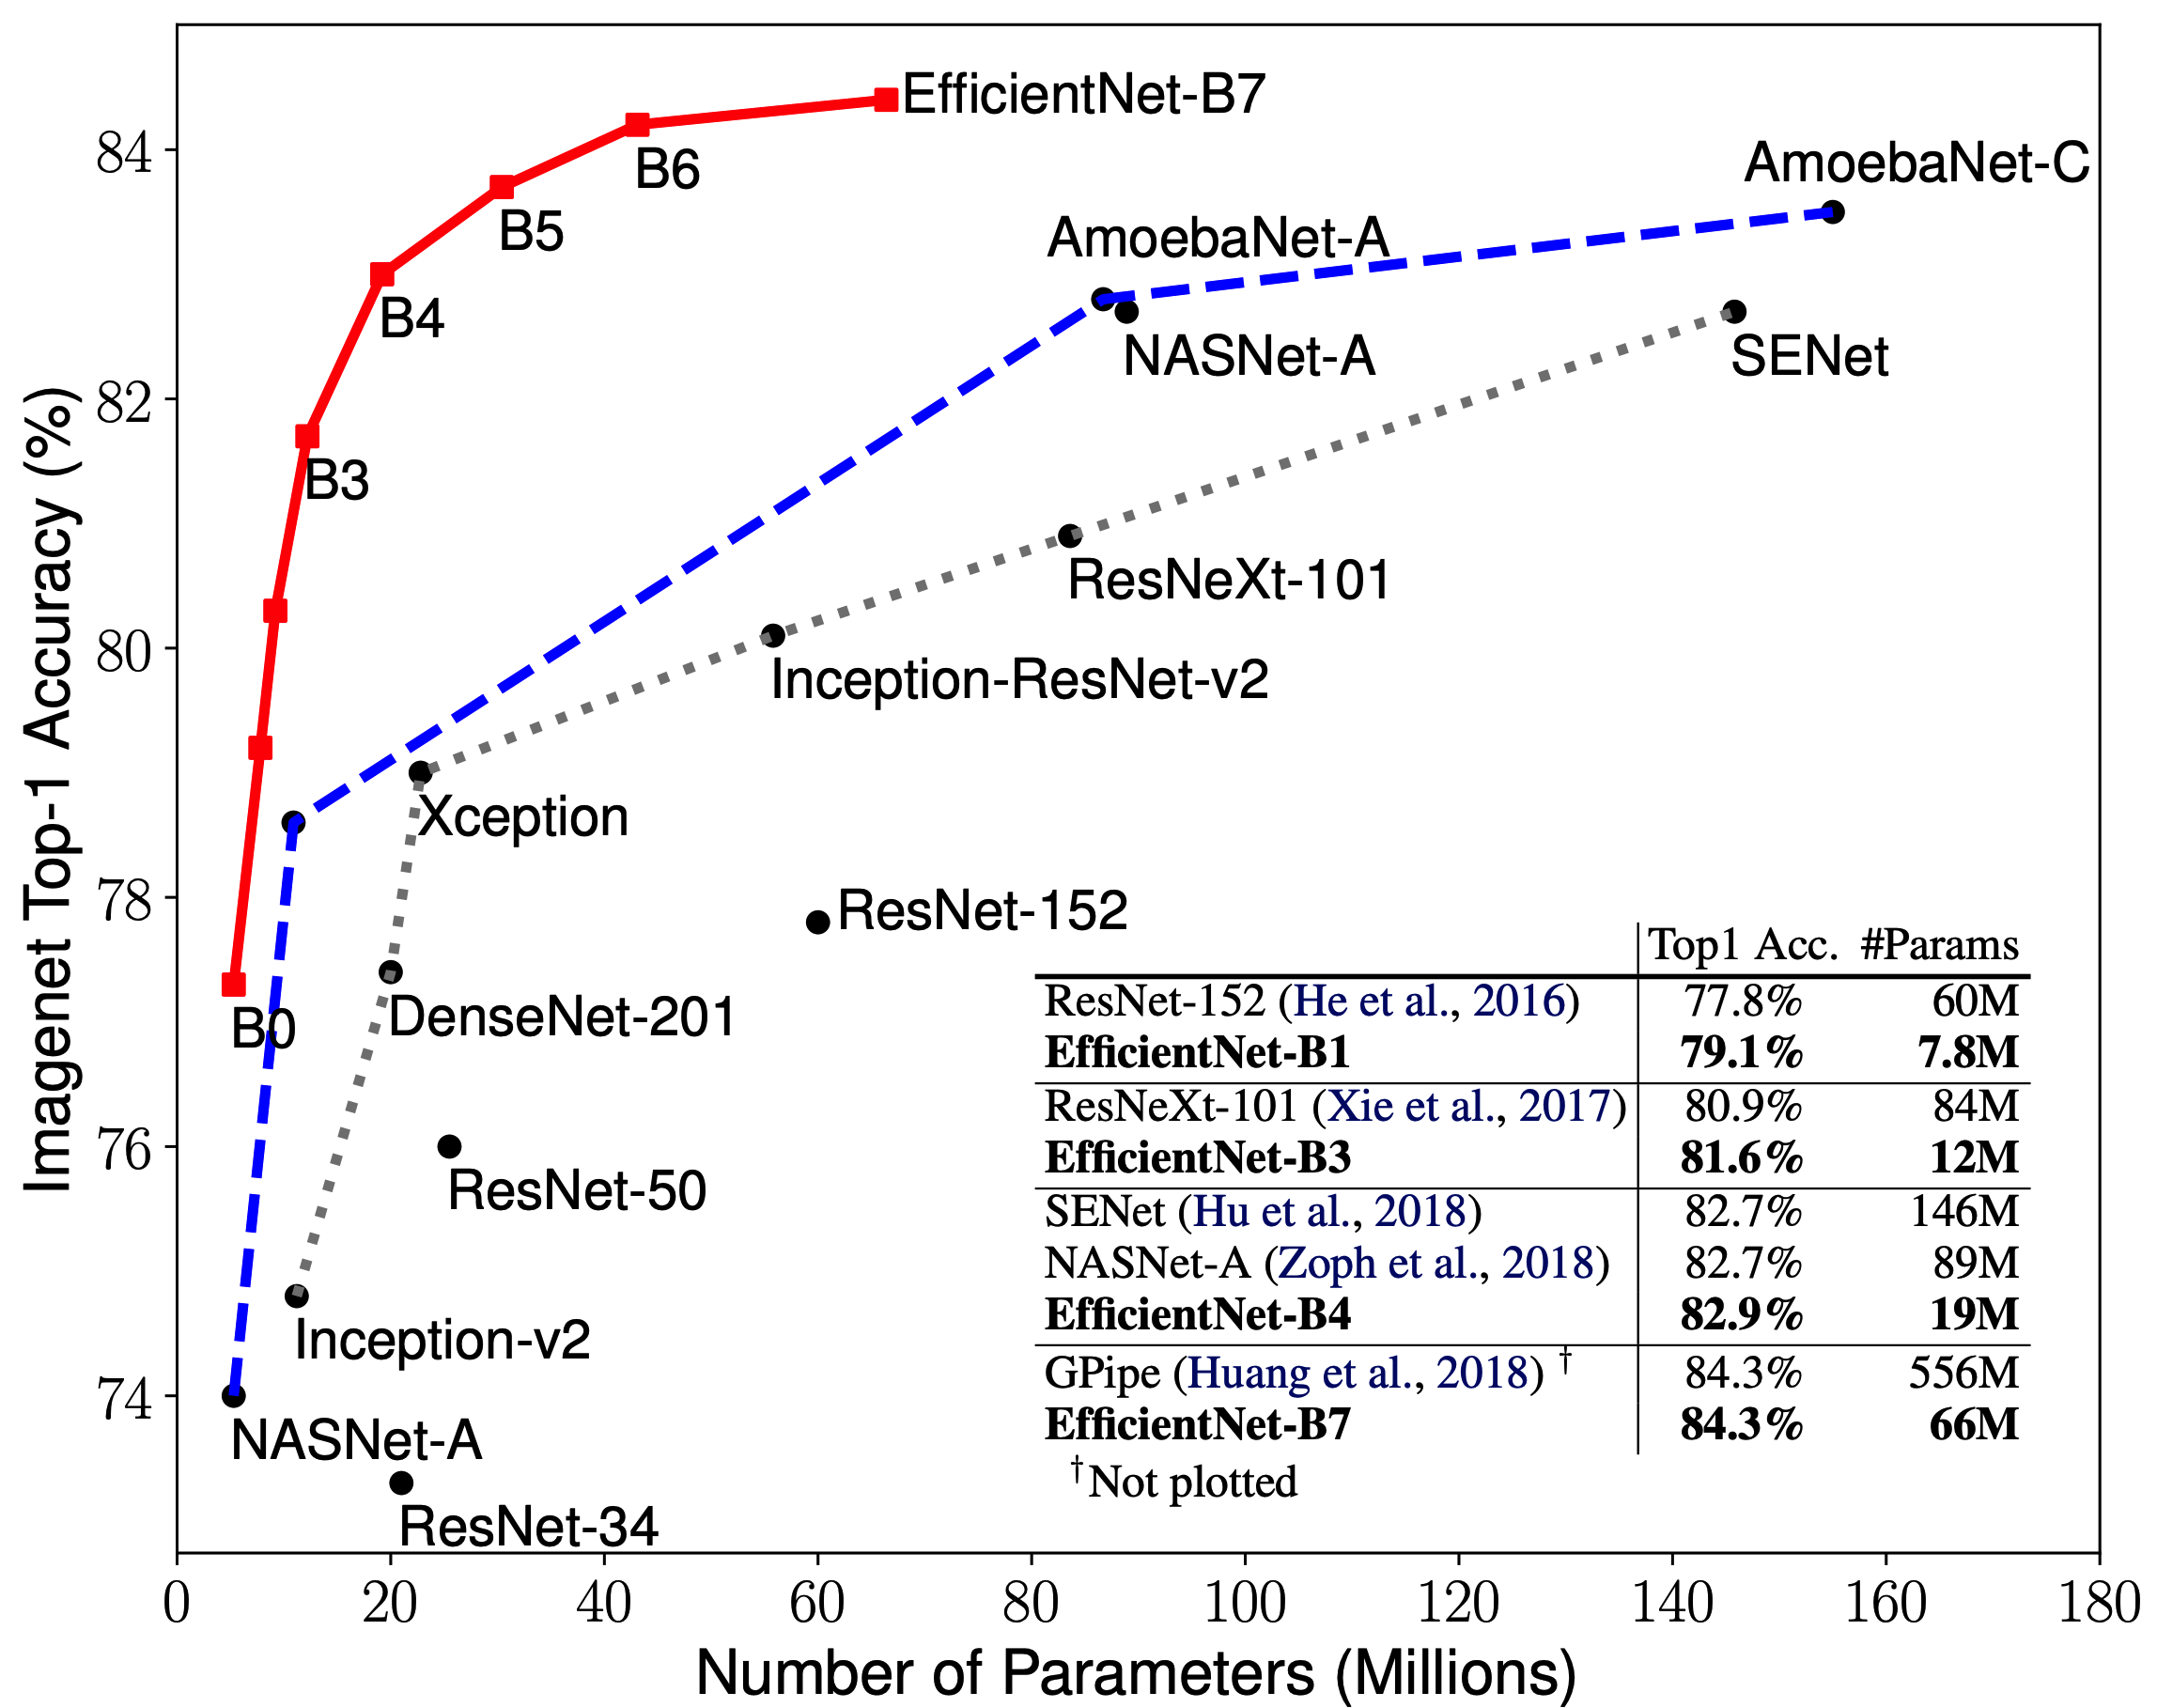
\includegraphics[width=0.7\linewidth]{pictures/ComparisonofEfficient.png}
    \caption{Comparison of EfficientNet with Different Networks on ImageNet\cite{219}}
    \label{fig:ComparisonofEfficient}
\end{figure}

To accommodate diverse detection-box sizes in practice, we adopt an intelligent scaling and padding strategy:\\
    (1) Aspect-ratio preserving scaling to avoid distortion;\\
    (2) Center placement on a 128×128 black canvas for uniform input size;\\
    (3) Data augmentation with horizontal flips, random rotations (±15°), color jitter, and random erasing to enhance generalization.\\
This preprocessing aligns training and inference distributions and mitigates domain shift. As shown in \textbf{Fig.}~\ref{fig:OverallFeatureExtraction}, the overall feature extraction and output process in our system is illustrated.
\begin{figure}[H]
    \centering
    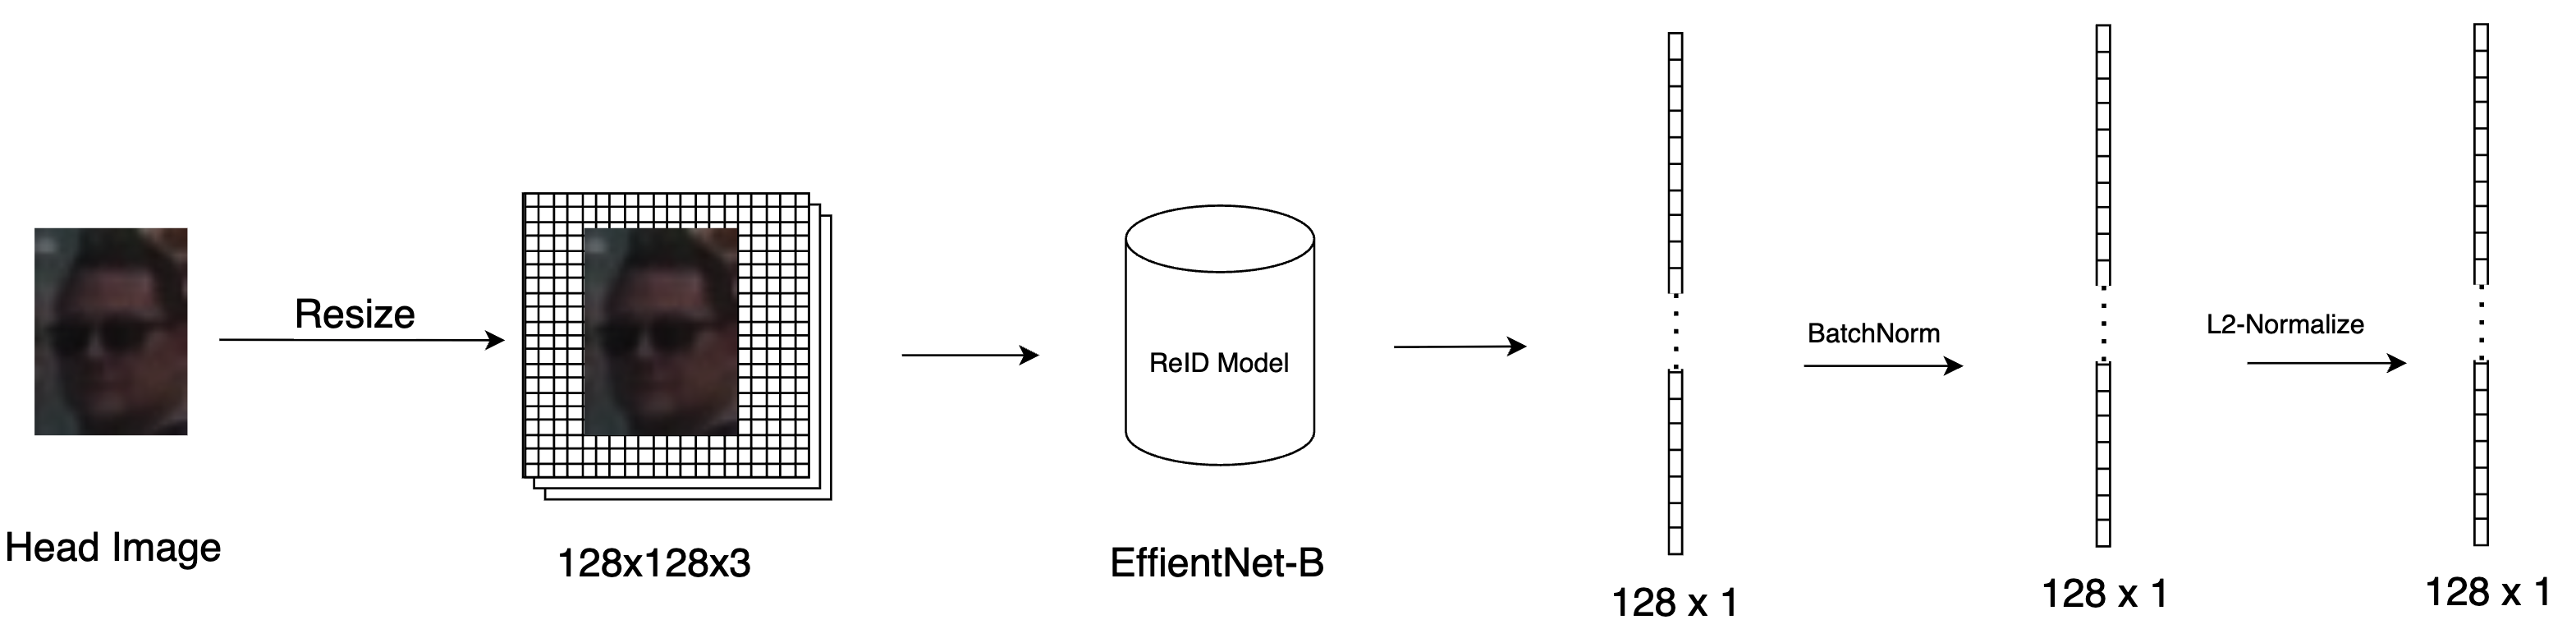
\includegraphics[width=0.9\linewidth]{pictures/OverallFeatureExtraction.png}
    \caption{Overall Feature Extraction and Output in Our System}
    \label{fig:OverallFeatureExtraction}
\end{figure}

For ReID, we use the triplet loss:
\begin{equation}
L_{triplet} = \max(0, d(a,p) - d(a,n) + \alpha)
\end{equation}
with $\alpha=0.5$. Training uses AdamW (lr=2×10⁻⁴, weight decay=1×10⁻⁴), OneCycleLR scheduling, mixed precision, and batch size 32.

\subsubsection{Data Association}
Data association matches detections to tracks by combining motion and appearance cues. The similarity measures include:\\
• Mahalanobis distance for motion compatibility: $D_M(i, j) = (d_j - y_i)^T S_i^{-1} (d_j - y_i)$, where $d_j$ is the detection, $y_i$ the prediction, and $S_i$ the covariance \cite{105}.\\
• Cosine distance for appearance: $D_C(i, j) = \min \{ 1 - \mathbf{r}_j^T \mathbf{r}_k^{(i)} \mid \mathbf{r}_k^{(i)} \in R_i \}$, where $R_i$ stores up to 100 recent descriptors per track \cite{105}.\\
• Combined cost: $c_{i,j} = \lambda D_M(i,j) + (1-\lambda) D_C(i,j)$ \cite{105}.\\
•Matching strategy:\\
(1)Cascaded matching prioritizes recently seen, longer-lived tracks to reduce ID switches under long occlusions \cite{134}.\\
(2) IoU matching as a fallback for remaining unmatched pairs.\\
(3) Hungarian algorithm solves the final assignment on the combined cost matrix \cite{103}.
\subsubsection{Track Management}
• Initialization: new detections start as "unconfirmed." After two consecutive matches, a track becomes confirmed.\\  
• Termination: tracks unmatched for a prolonged period (e.g., beyond max\_age) are removed.\\
• ID retention and re-identification: combined motion and appearance cues enable re-identification after temporary disappearance; prolonged absence may result in a new ID.

\subsection{Adaptivity Across Scenarios}
Parameters of Kalman filtering (state model, Q, R), gating thresholds, cost weighting, cascade/IoU matching, track lifecycle (n\_init, max\_age), and ReID strength should be tuned to scene characteristics (e.g., irregular motion, noisy detections, frequent occlusion, similar appearances) to maintain robustness.

\subsection{Counting Method}
In our method, given YOLOv11 detections and DeepSORT trajectories, we design a reliable counting algorithm that avoids double-counting. Pure detection summation over frames would overcount the same target repeatedly; counting must therefore operate on unique track IDs.

\subsubsection{Traditional line-crossing and limitations}
The mainstream approach is line/zone crossing \cite{22_hsu_passenger_2020, 204, 68_zhao_detection_2022}, which triggers a count when a trajectory crosses a virtual line. In crowded scenes, brief occlusions near the line can cause severe undercounting (e.g., three people cross abreast but the middle person is fully occluded). As shown in our ablations (\textbf{Chapter} 5), a zero-width line (bandwidth 0) can yield MAPE as high as 93.43%.

\subsubsection{Virtual counting band (ours)}
We propose a Virtual Counting Band with nonzero width near the left/right image borders (\textbf{Fig.}~\ref{fig:VirtualCountingZone}), defined by start/end boundaries as proportions of image width. A target is counted only if it is continuously observed within the band for a preset number of frames. This design:
\begin{itemize}
    \item \textbf{Improves robustness}: a buffer region tolerates brief occlusions and detection jitter;
    \item \textbf{Stabilizes counting}: avoids repeated or spurious counts due to oscillations around a thin line.
\end{itemize}

\begin{figure}[H]
    \centering
    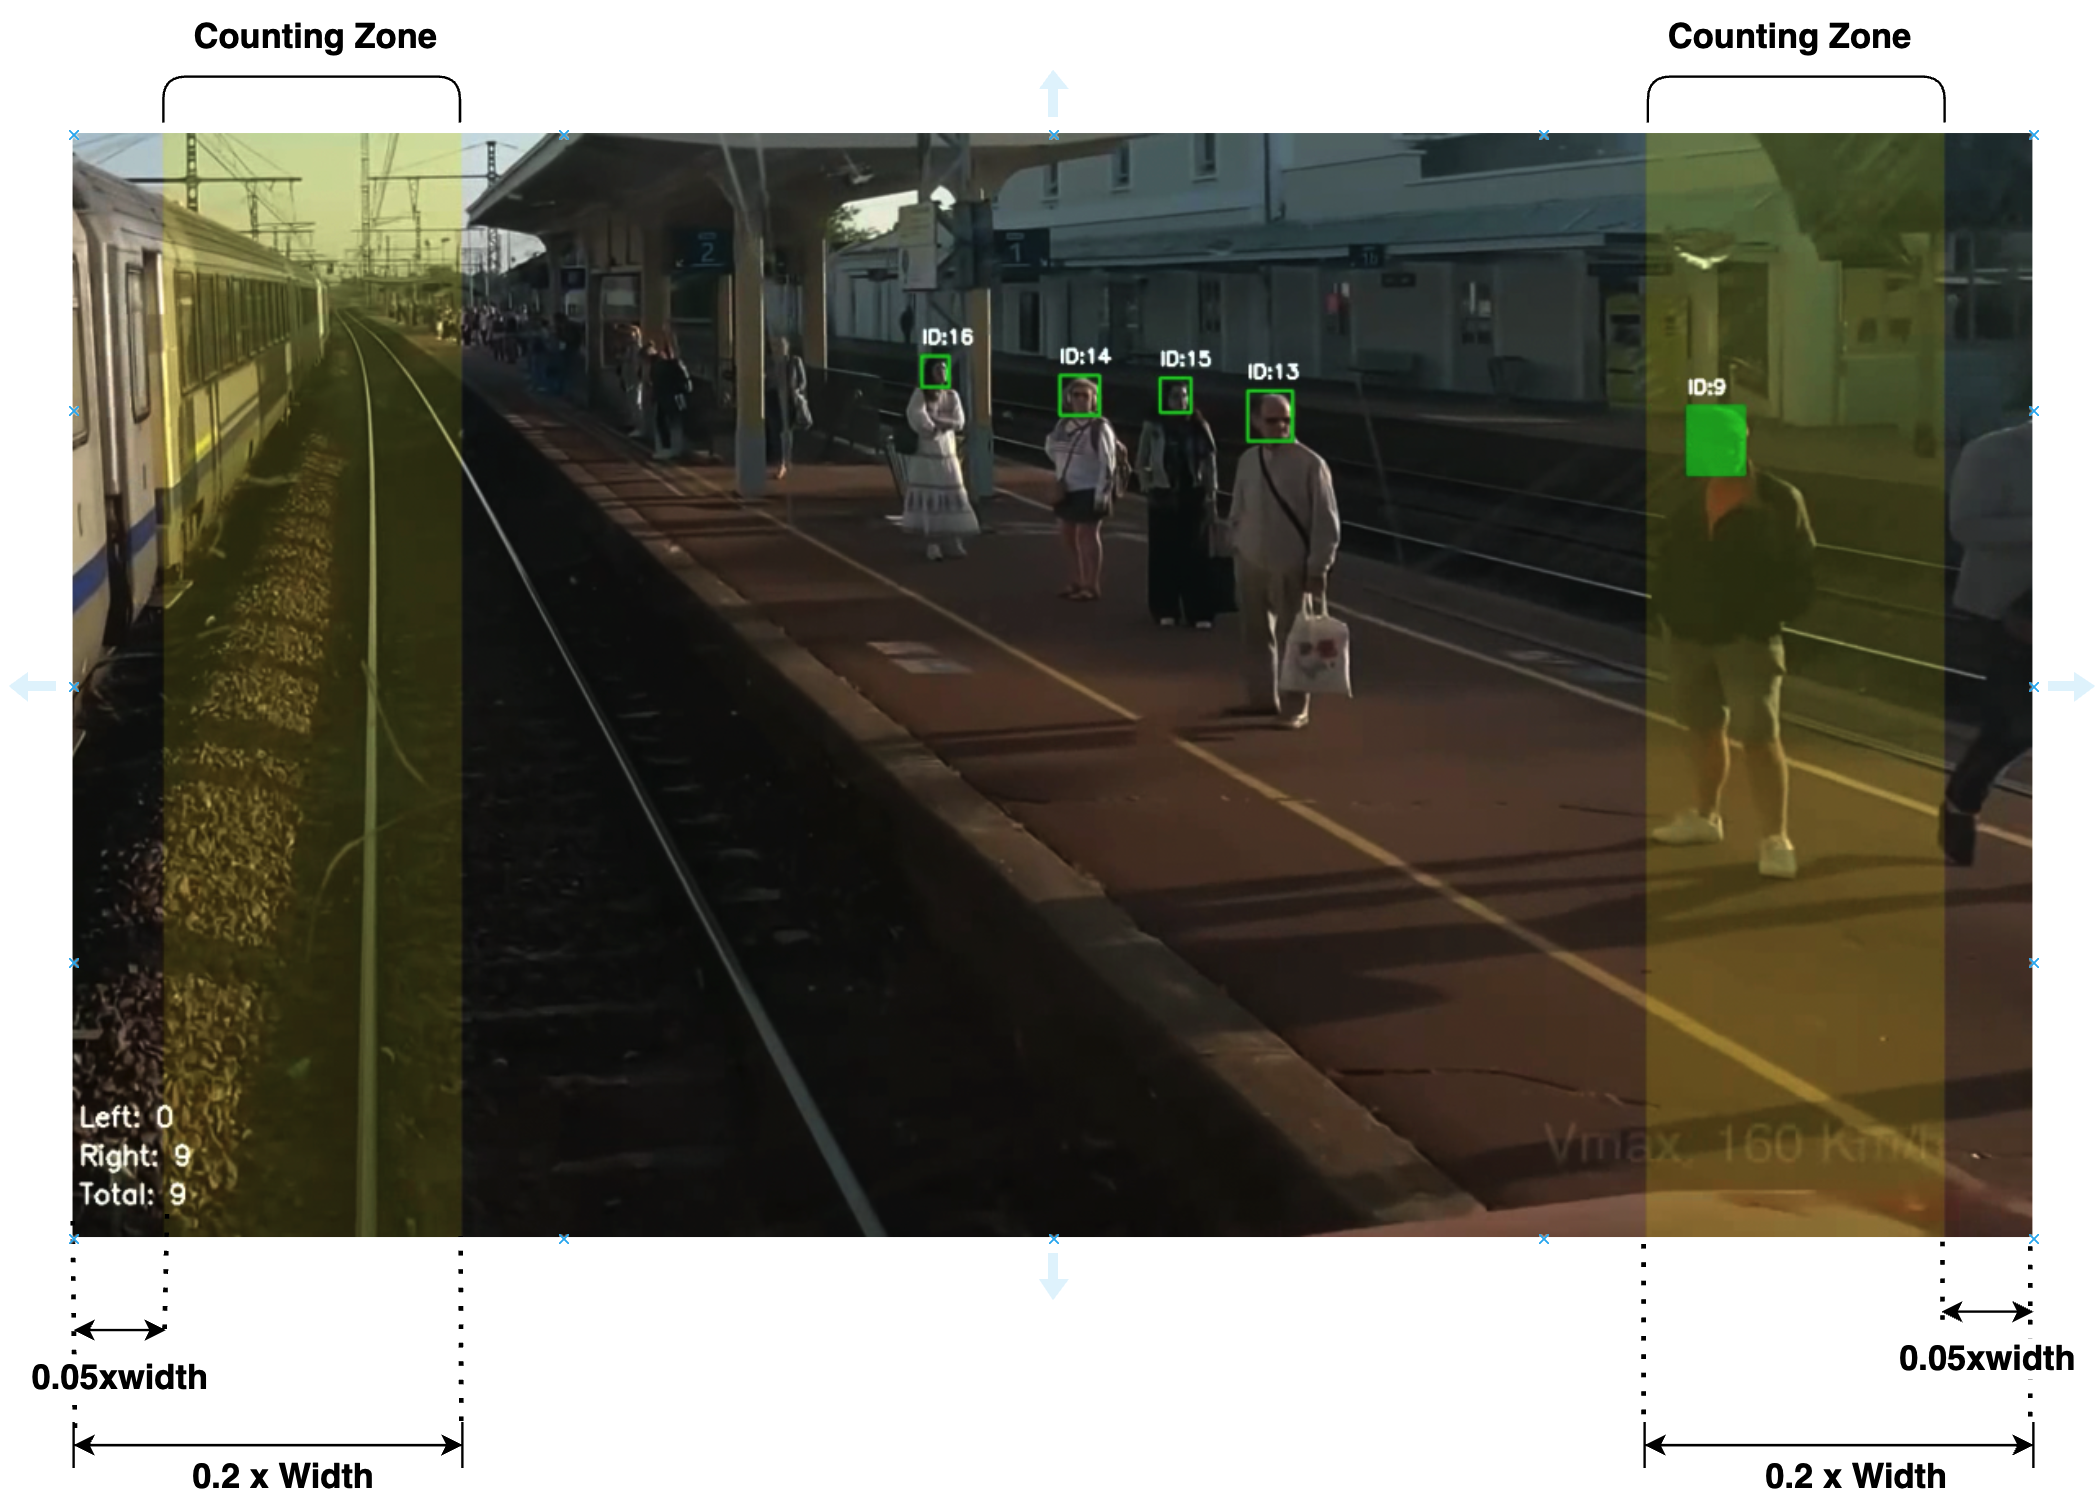
\includegraphics[width=0.7\textwidth]{pictures/VirtualCountingZone.png}
    \caption{Virtual Counting Band Illustration}
    \label{fig:VirtualCountingZone}
\end{figure}
In practice, we set the band to 5\%–20\% of the width from the image borders (relative coordinates for resolution invariance). We maintain per-track state (consecutive in-band frames, counted flag). The target position is the box center; boxes partially outside the frame are clipped for display while preserving original coordinates for logic.

\textbf{Algorithm Implementation:}
\begin{enumerate}
    \item \textbf{Track State Management:} For each confirmed track, maintain state variables: consecutive\_in\_band\_frames, counted\_flag, and side\_assignment (left/right).
    \item \textbf{Band Membership Test:} Compute bounding box center $(u,v)$ and test if $u \in [\text{Start} \cdot W, \text{End} \cdot W]$ for left band or $u \in [W - \text{End} \cdot W, W - \text{Start} \cdot W]$ for right band.
    \item \textbf{Persistence Logic:} If track is in band, increment consecutive\_in\_band\_frames; otherwise reset to 0. When consecutive\_in\_band\_frames $\geq N$ (default N=2) and counted\_flag=False, set counted\_flag=True and increment corresponding side counter.
    \item \textbf{Deduplication:} Maintain global set of counted\_IDs to prevent double-counting across frames.
    \item \textbf{End-of-Video Compensation:} For tracks with consecutive\_in\_band\_frames $> 0$ but $< N$ at video end, apply compensation rule: if consecutive\_in\_band\_frames $\geq N/2$, count the track.
    \item \textbf{Final Aggregation:} Report left count, right count, and final count = max(left\_count, right\_count) to avoid non-platform bias.
\end{enumerate}

Integrity mechanisms include: \\
(1) end-of-video compensation to include targets that nearly meet the persistence threshold; 
(2) deduplication by maintaining the set of counted IDs;\\
(3) using the maximum of left/right counts as the final result (we count one side), which avoids bias from non-platform-side flows.



\subsection{Assumptions and Limitations}
Our formulation assumes: (i) a forward-looking camera with intrinsics $(f,c_x,c_y)$ estimated from representative frames; (ii) average head height $H$ suitable for platform pedestrians; (iii) along-track deceleration during arrivals consistent with the kinematic model. Performance may degrade under extreme lighting or ultra-dense scenes that increase appearance ambiguity or violate motion smoothness. These assumptions are reflected in the calibration and evaluation reported in Chapter~5.

\subsection{Evaluation Metrics}

\subsubsection{Detection Metrics}
We report head detection performance on a static validation set using mAP@0.5 and Recall \cite{74_yolo11_Jocher_Ultralytics_YOLO_2023}. Formally:\\
\textbf{mAP50}: mean AP at IoU threshold 0.5,\\
\begin{equation}
\text{mAP50} = \frac{1}{N}\sum_{i=1}^{N}\text{AP}_i \quad \text{at IoU threshold of 0.5}
\end{equation}
\textbf{mAP50-95}: mean AP averaged over IoU thresholds from 0.5 to 0.95 in steps of 0.05,\\
\begin{equation}
\text{mAP50-95} = \frac{1}{10}\sum_{t=0.5}^{0.95}\text{mAP}_t
\end{equation}
\textbf{Box Precision} and \textbf{Recall} are\\
\begin{equation}
\text{Precision} = \frac{TP_{\text{box}}}{TP_{\text{box}} + FP_{\text{box}}}, \quad
\text{Recall} = \frac{TP_{\text{box}}}{TP_{\text{box}} + FN_{\text{box}}}.
\end{equation}

\subsubsection{Tracking Metrics}
On MOT-RPCH we adopt MOTChallenge metrics: IDF1, MOTA, IDSW, Mostly Tracked(MT), Partially Tracked(PT), Mostly Lost(ML). Following CLEAR-MOT and ID-based protocols (\texttt{py-motmetrics \cite{py-motmetrics} }):\\
\paragraph{CLEAR-MOT}
\begin{align}
\text{MOTA} &= 1 - \frac{\sum_t (FN_t + FP_t + IDSW_t)}{\sum_t GT_t}, \\
\text{MOTP} &= \frac{\sum_{i,t} d_{i,t}}{\sum_t TP_t},
\end{align}
where $GT_t$ is the number of ground-truth objects at time $t$, and $d_{i,t}$ is the distance between a matched hypothesis and ground truth.
\paragraph{Identity-based}
\begin{align}
\text{ID Precision (IDP)} &= \frac{IDTP}{IDTP + IDFP}, \\
\text{ID Recall (IDR)} &= \frac{IDTP}{IDTP + IDFN}, \\
\text{IDF1} &= \frac{2 \cdot IDTP}{2 \cdot IDTP + IDFP + IDFN}.
\end{align}
Additional measures: $IDSW$, Matches, $FP$, $FN$, FAF $= \frac{\sum_t FP_t}{\text{\#frames}}$, and standard Precision/Recall. Track quality: Mostly Tracked (MT, $\geq$80\%), Partially Tracked (PT, 20\%--80\%), Mostly Lost (ML, $<$20\%).

\subsubsection{Counting Metrics}
For $N$ test videos with predicted unique count $\hat{C}_i$ and ground truth $C_i$:
\begin{align}
\text{MAE} &= \frac{1}{N} \sum_{i=1}^{N} | \hat{C}_i - C_i |, \\
\text{RMSE} &= \sqrt{\frac{1}{N} \sum_{i=1}^{N} (\hat{C}_i - C_i)^2}, \\
\text{MAPE} &= \frac{100\%}{N} \sum_{i=1}^{N} \frac{|\hat{C}_i - C_i|}{C_i}, \\
\text{ME} &= \frac{1}{N} \sum_{i=1}^{N} (\hat{C}_i - C_i).
\end{align}



\paragraph{Mean Absolute Error (MAE)} MAE quantifies the average magnitude of the discrepancy between predicted counts and their ground-truth counterparts. Computed as the arithmetic mean of absolute deviations across all samples, MAE offers two key advantages: (i) interpretability—its value directly reflects the mean absolute deviation of estimates from true counts; and (ii) robustness—by imposing a linear penalty on each residual, MAE remains insensitive to outliers and thus delivers a stable summary of overall model performance.

\paragraph{Root Mean Squared Error (RMSE)} RMSE is a widely adopted metric for assessing prediction accuracy. In contrast to MAE, RMSE squares the residuals before averaging and subsequent square-rooting. This quadratic penalty disproportionately amplifies large errors, making RMSE markedly more sensitive to extreme deviations. Consequently, RMSE is the metric of choice when large mispredictions incur disproportionately high costs or when model behavior under adverse conditions must be critically evaluated. By construction, RMSE ≥ MAE; the divergence between the two statistics exposes the presence of occasional large-scale prediction failures.

\paragraph{Mean Absolute Percentage Error (MAPE)} MAPE measures relative, rather than absolute, prediction error. For each sample, the absolute error is normalized by the ground-truth count and expressed as a percentage; MAPE is the average of these percentage errors. Being scale-free, MAPE enables equitable comparison across datasets with disparate count ranges and is particularly informative when performance must remain consistent across both sparse and dense regions. A caveat arises when the true count $C_i$ approaches zero, causing the percentage to explode and rendering MAPE unstable or undefined.

\paragraph{Mean Error (ME), interchangeably termed Bias} ME, interchangeably termed Bias, captures systematic deviation of predictions. It is defined as the average signed difference between estimated and true counts. A positive ME indicates a persistent over-counting tendency, whereas a negative ME signals chronic under-counting. Unlike MAE and RMSE, which quantify error magnitudes, ME diagnoses directional drift and is indispensable for calibrating models to eliminate systematic offsets in safety-critical or metrologically sensitive applications.


\clearpage
\section{Experiments and Results}\label{section::Experiments and Results}


This chapter systematically evaluates the proposed head detection, platform-scene multi-object tracking, and counting framework following the detect–track–count pipeline. We adopt YOLOv11m as the detector, an EfficientNet-B0 based ReID appearance descriptor, and three motion models within the DeepSORT framework: the standard 8-dimensional constant-velocity baseline (classic DeepSORT Kalman filter), a 12-dimensional constant-acceleration model, and a 5-dimensional physics-constrained model based on pinhole camera geometry. Evaluations are conducted on MOT-formatted data curated in the Data chapter; the detector's training and fine-tuning leverage complementary static images and multi-clip video sequences, covering both generic crowded scenes and platform scenarios with varying densities during train arrivals.


\subsection{Training and Fine-tuning of the YOLOv11m Detector}
As discussed in Chapter 4, we use YOLOv11m as a balanced choice between accuracy and speed. We adopt a two-stage transfer learning strategy to build a head detector with strong generalization and high performance in our target domain, thereby providing reliable inputs to downstream tracking. Stage 1 pre-trains on CrowdHuman to learn generic head features; Stage 2 fine-tunes with backbone=10 frozen on 2,000 labeled head images drawn from Open Sensor Data for Rail 2023, RailEye3D, and our TrainPlatformCrowd datasets, yielding YOLO11freeze10.pt.

The hyperparameters are as follows: both stages train for 100 epochs using SGD (initial lr=0.01, momentum=0.937, weight decay=0.0005). Other parameters follow YOLO defaults.

The pre-training objective is to learn robust, generic head features from a large-scale, diverse dataset. We therefore use CrowdHuman, which provides abundant instances for deep networks (see Chapter 3). The pre-training results on CrowdHuman are shown in Figure~\ref{fig:yolo11mpre2results} and Table~\ref{tab:yolopre2_results}: mAP50=79.4\% and mAP50–95=54.7\%.
\begin{figure}[H]
    \centering
    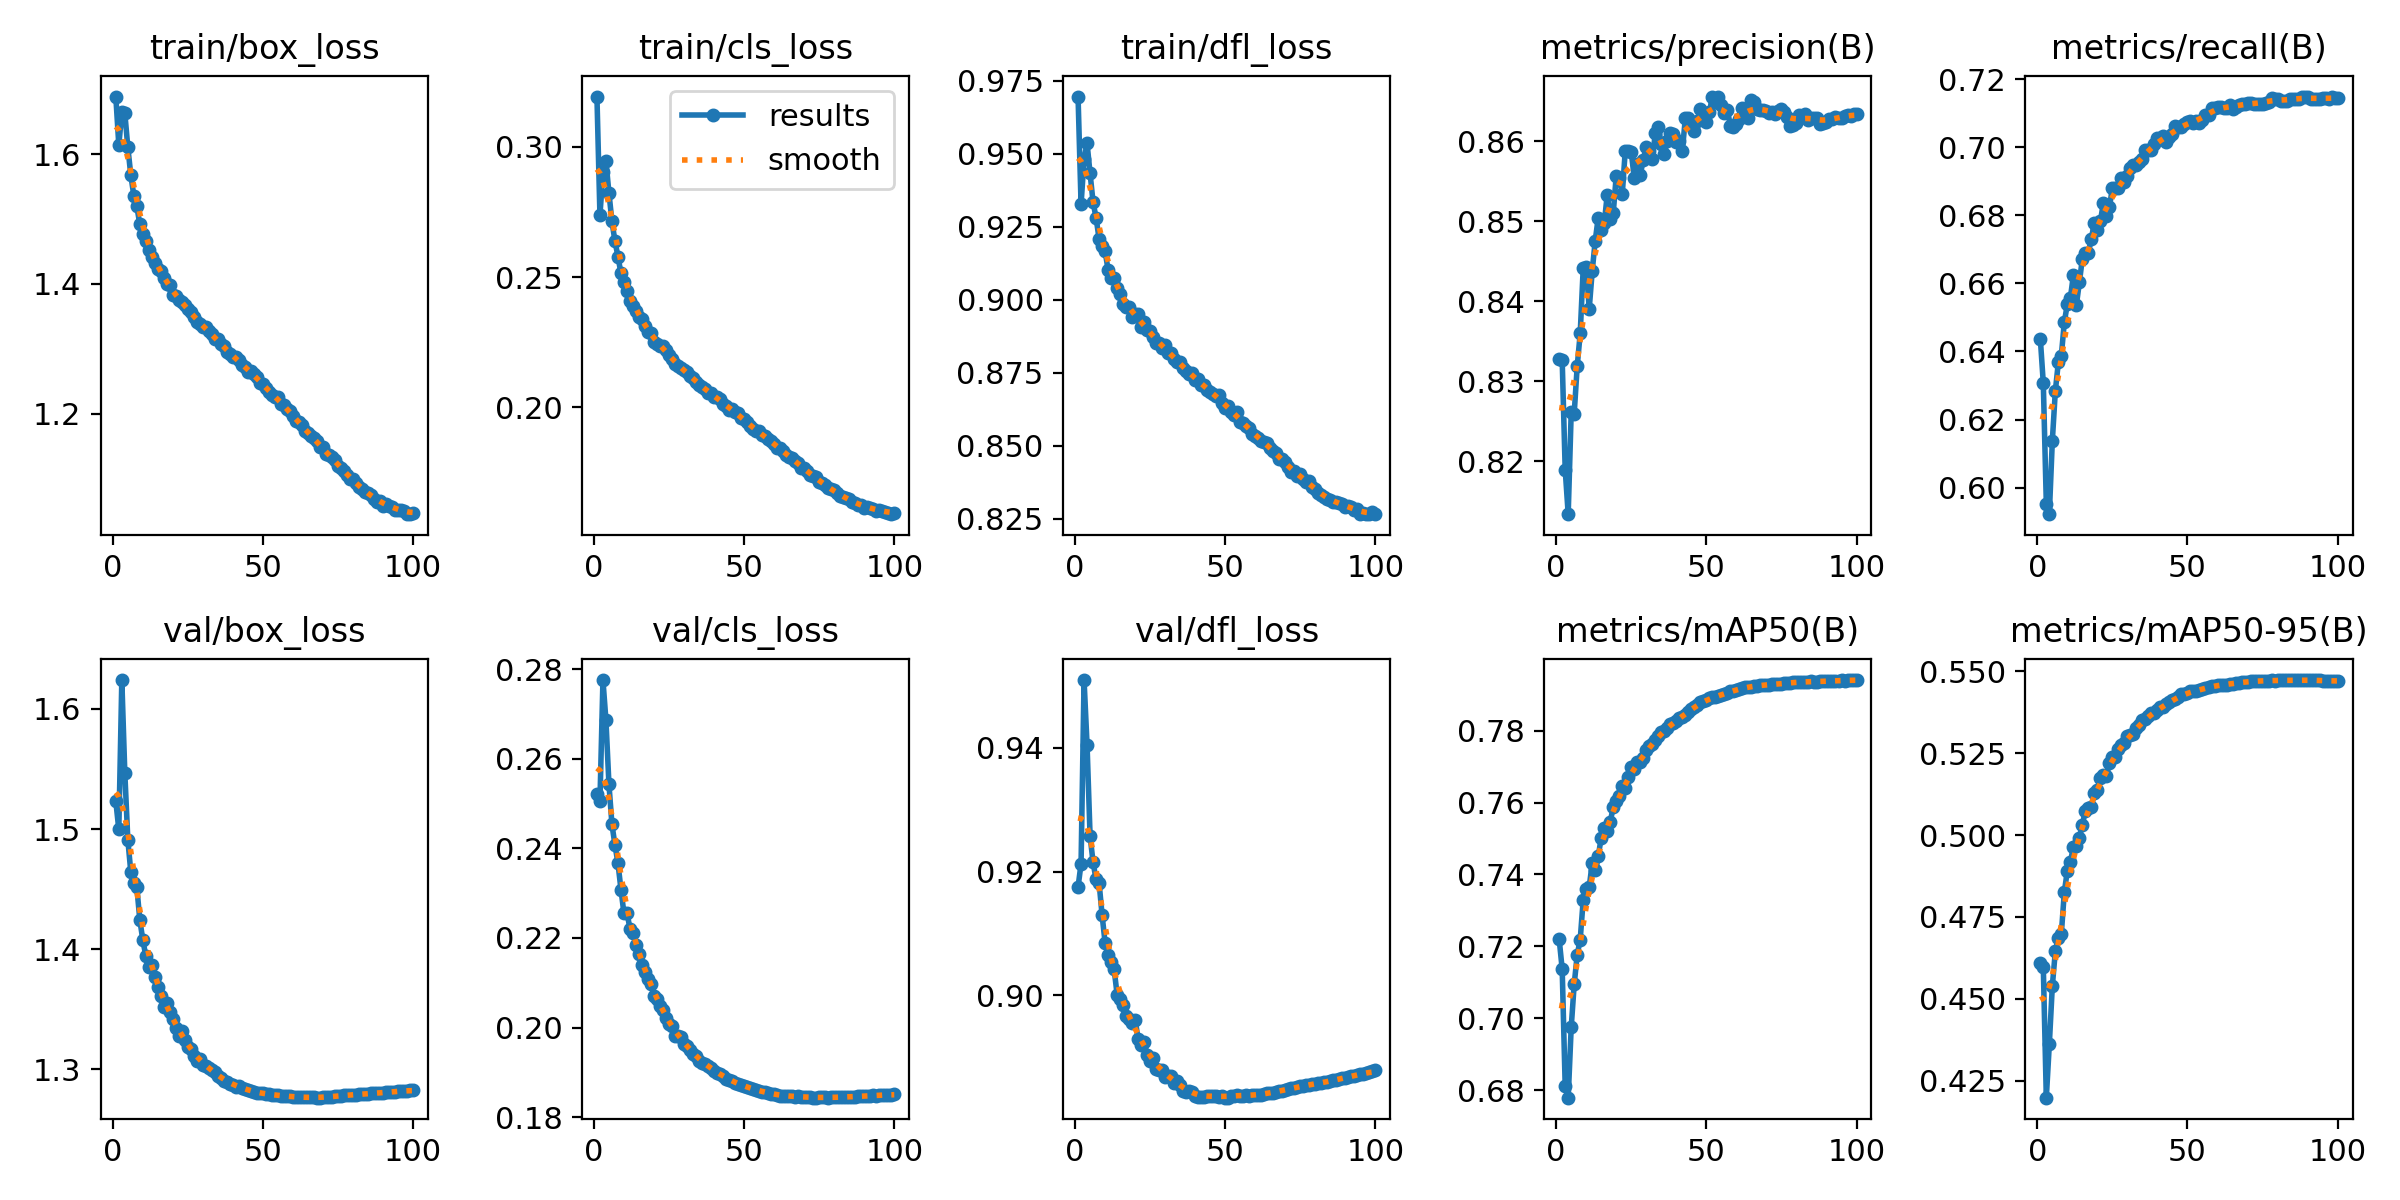
\includegraphics[width=0.8\textwidth]{pictures/yolo11mpre2results.png}
    \caption{Pre-training Results of YOLOv11m on the CrowdHuman Dataset}
    \label{fig:yolo11mpre2results}
\end{figure}

\begin{table}[H]
\centering
\resizebox{0.8\textwidth}{!}{%
\setlength{\tabcolsep}{12pt}
\renewcommand{\arraystretch}{1.3}
\begin{tabular}{|c|c|c|c|c|c|c|}
\hline
\textbf{Class} & \textbf{Images} & \textbf{Instances} & \textbf{Box(Precision)} & \textbf{Recall} & \textbf{mAP50} & \textbf{mAP50–95} \\
\hline
all & 4370 & 98568 & 0.862 & 0.715 & 0.794 & 0.547 \\
\hline
\end{tabular}%
}
\caption{Pre-training Performance of YOLOv11m on the CrowdHuman Dataset}
\label{tab:yolopre2_results}
\end{table}
These results indicate that the model has learned basic head detection capability: mAP50 reflects performance under a lenient IoU threshold, whereas mAP50–95 averages over stricter thresholds, better capturing localization quality. While pre-training establishes a solid foundation, localization in complex scenes still has room to improve.

Stage 2 conducts domain adaptation via fine-tuning. We freeze the first 10 backbone layers to retain generic low-level features (edges, colors, textures) learned from CrowdHuman and avoid catastrophic forgetting on smaller domain data. Training focuses on deeper layers to learn platform-specific semantics (illumination, occlusion patterns, crowd layouts). Results in Figure~\ref{fig:yolo11mfinetuneresults} and Table~\ref{tab:yolofreeze10_results} show substantial gains: mAP50 improves from 79.4\% to 98.0\% (+18.6 points), and mAP50–95 from 54.7\% to 81.6\% (+26.9 points). The large mAP50–95 improvement highlights markedly better localization, which is critical for reducing ID switches and trajectory drift in downstream tracking.
\begin{figure}[H]
    \centering
    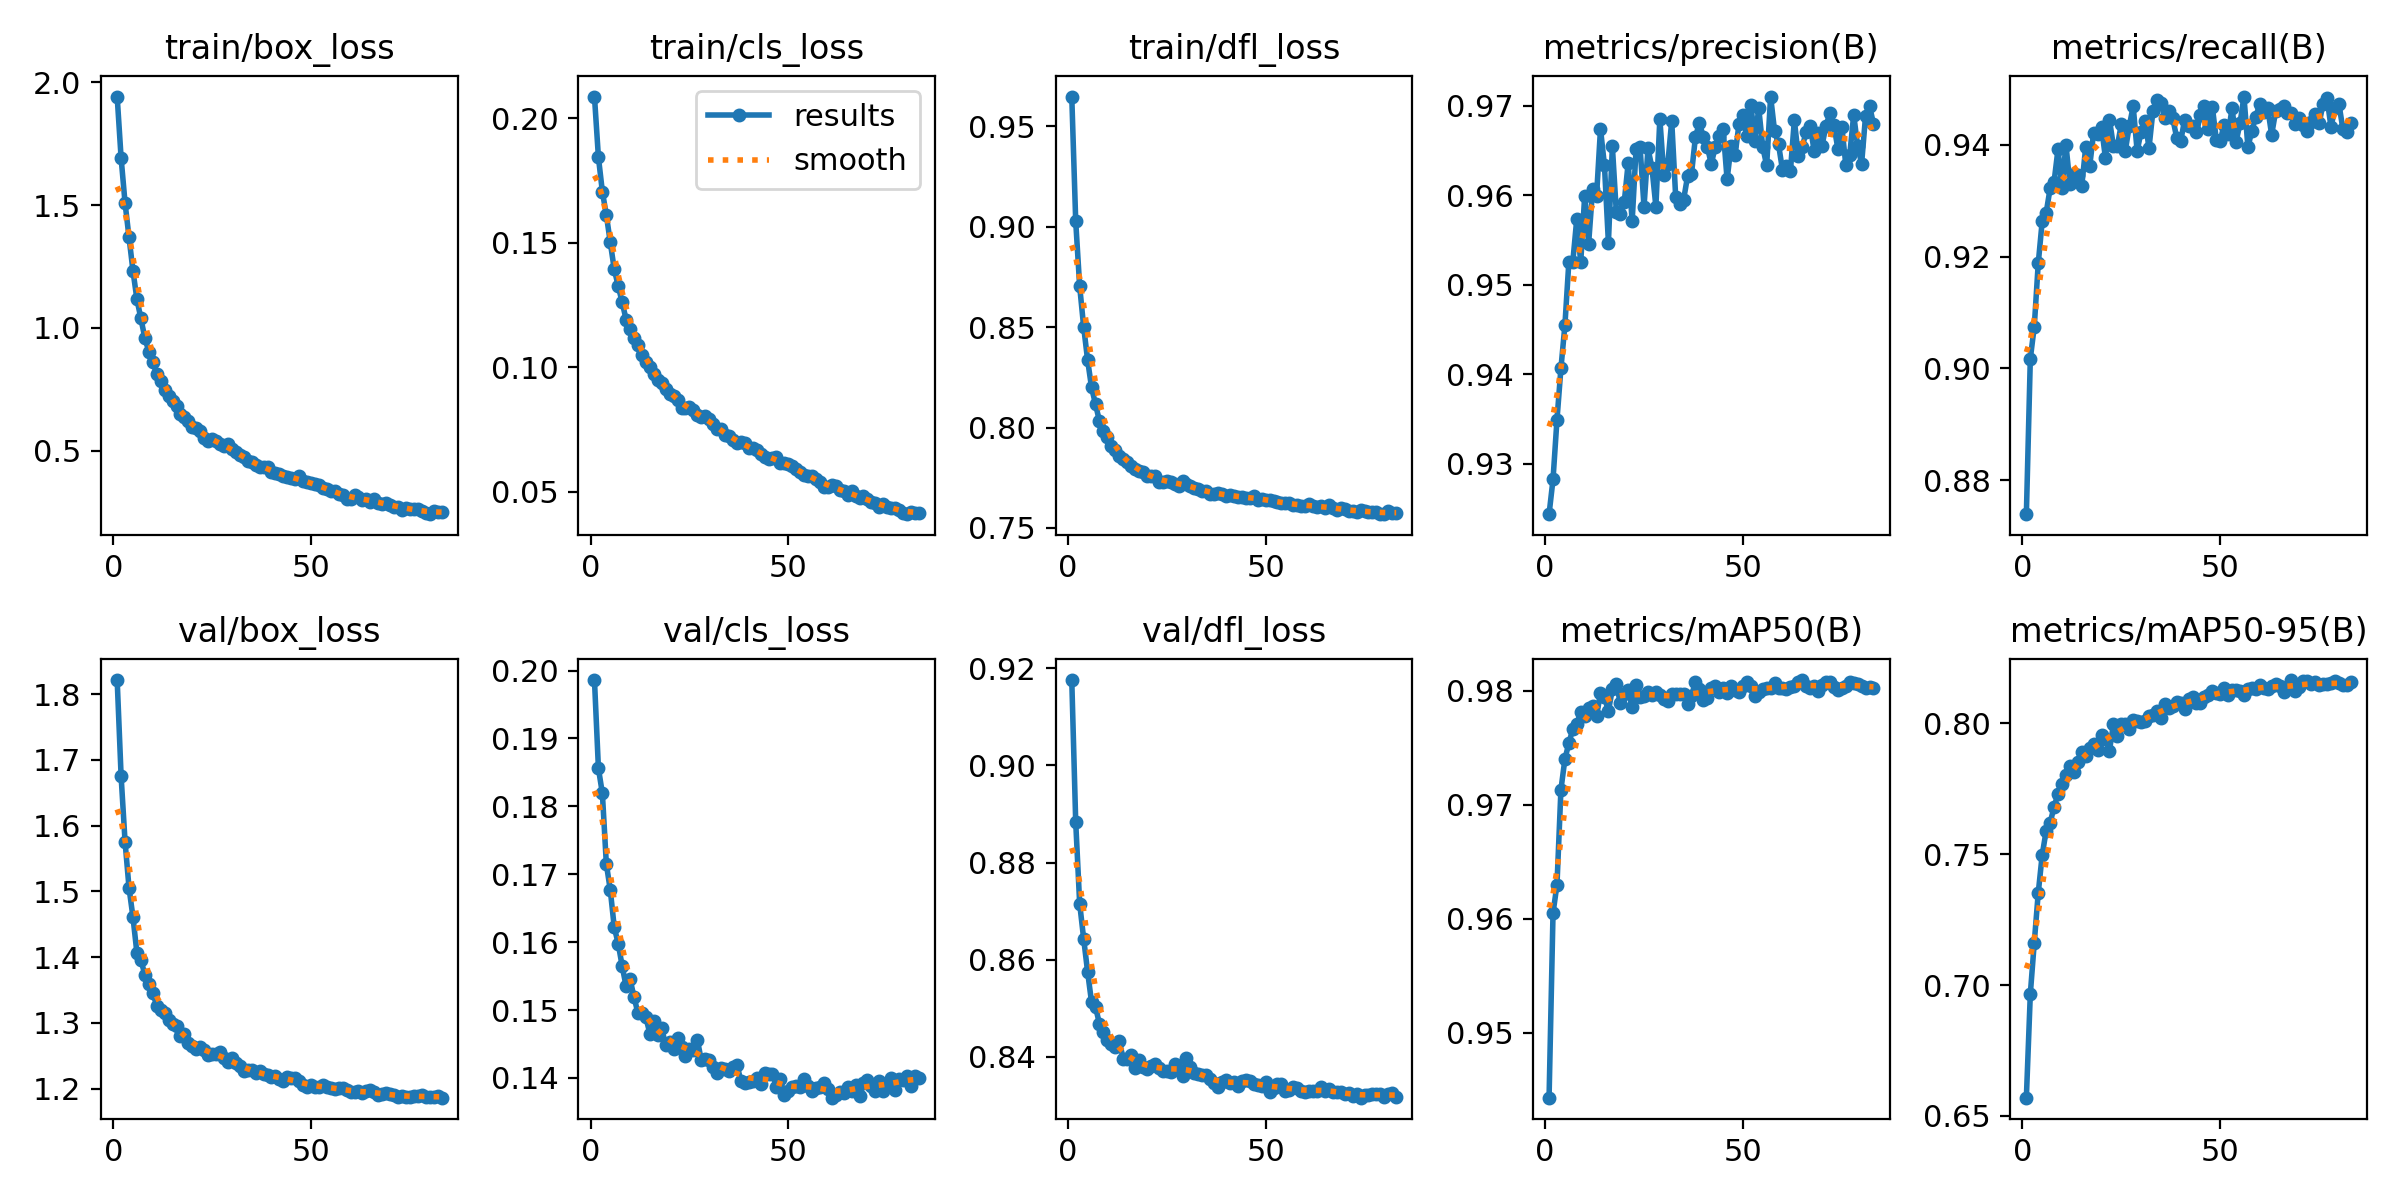
\includegraphics[width=0.8\textwidth]{pictures/yolofreez10_ResultsSummary.png}
    \caption{Fine-tuning Results of YOLOv11m on the Custom Head Dataset}
    \label{fig:yolo11mfinetuneresults}
\end{figure}

\begin{table}[H]
\centering
\resizebox{0.8\textwidth}{!}{%
\setlength{\tabcolsep}{12pt}
\renewcommand{\arraystretch}{1.3}
\begin{tabular}{|c|c|c|c|c|c|c|}
\hline
\textbf{Class} & \textbf{Images} & \textbf{Instances} & \textbf{Box(P)} & \textbf{R} & \textbf{mAP50} & \textbf{mAP50–95} \\
\hline
all & 600 & 4779 & 0.965 & 0.946 & 0.980 & 0.816 \\
\hline
\end{tabular}%
}
\caption{Fine-tuning Performance of YOLOv11freeze10 on the Labeled Head Dataset}
\label{tab:yolofreeze10_results}
\end{table}
In summary, the two-stage strategy transforms YOLOv11m from a generic head detector into a platform-optimized high-performance detector (YOLOv11freeze10.pt), providing strong inputs for subsequent tracking and counting.


\subsubsection{Detector Ablation Study}
We design an ablation study to examine the fine-tuned detector's sensitivity to hyperparameters. All experiments are conducted on the same T4 GPU environment and evaluated on a shared 2,071-image validation set constructed from MOT-annotated video frames, ensuring consistency and application relevance.

We vary three key hyperparameters—input size, confidence threshold, and IoU threshold—as follows:
\begin{table}[H]
    \centering
    \begin{tabular}{|c|c|c|c|c|}
    \hline
        \textbf{Conf} & 0.3 & 0.5 & 0.7 & 0.9  \\ \hline
        \textbf{IoU} & 0.3 & 0.5 & 0.7 & 0.9  \\ \hline
        \textbf{Imgsz} & 640 & 736 & 832 & 960 \\ \hline
    \end{tabular}
    \caption{Detector ablation parameters Setting}
    \label{Detector ablation parameters}
\end{table}
This yields 64 combinations. Results are summarized in Table~\ref{tab:T25_YOLO11m_Ablation}. The best performance is achieved with conf=0.3, iou=0.3, imgsz=736, balancing precision–recall and feature resolution–compute trade-offs. A lower confidence threshold preserves more potential positives, an intermediate IoU threshold reduces duplicates without excessive suppression, and 736 px affords sufficient spatial detail for small heads while controlling cost. The configuration notably improves mAP50–95, indicating robust performance across IoU thresholds and suitability for real-world deployment.


\begin{table}[H]
    \centering
    \resizebox{0.7\textwidth}{!}{%
    \scriptsize
    \renewcommand{\arraystretch}{1.3}
    \begin{tabular}{ccccccccc}
    \hline
        \textbf{No.} & \textbf{Conf} & \textbf{IoU} & \textbf{Imgsz} & \textbf{mAP50} & \textbf{mAP50-95} & \textbf{Precision} & \textbf{Recall} & \textbf{Inference\_Time(ms) } \\ \hline
        1 & 0.3 & 0.3 & 640 & 0.9248  & 0.6749  & 0.9272  & 0.8741  & 13.18   \\ 
        \rowcolor{gray!10}
        2 & 0.3 & 0.3 & 736 & 0.9224  & 0.6871  & 0.9193  & 0.8707  & 16.86   \\ 
        3 & 0.3 & 0.3 & 832 & 0.8997  & 0.6545  & 0.9195  & 0.8238  & 21.79   \\ 
        \rowcolor{gray!10}
        4 & 0.3 & 0.3 & 960 & 0.8664  & 0.6144  & 0.8947  & 0.7786  & 29.42   \\ 
        5 & 0.3 & 0.5 & 640 & 0.9247  & 0.6748  & 0.9246  & 0.8745  & 14.63   \\ 
        \rowcolor{gray!10}
        6 & 0.3 & 0.5 & 736 & 0.9224  & 0.6869  & 0.9177  & 0.8712  & 18.18   \\ 
        7 & 0.3 & 0.5 & 832 & 0.8997  & 0.6543  & 0.9183  & 0.8243  & 23.32   \\ 
        \rowcolor{gray!10}
        8 & 0.3 & 0.5 & 960 & 0.8661  & 0.6143  & 0.9003  & 0.7736  & 31.44   \\ 
        9 & 0.3 & 0.7 & 640 & 0.9244  & 0.6744  & 0.9316  & 0.8652  & 14.44   \\ 
        \rowcolor{gray!10}
        10 & 0.3 & 0.7 & 736 & 0.9220  & 0.6865  & 0.9120  & 0.8717  & 18.05   \\ 
        11 & 0.3 & 0.7 & 832 & 0.8991  & 0.6538  & 0.9146  & 0.8242  & 23.43   \\ 
        \rowcolor{gray!10}
        12 & 0.3 & 0.7 & 960 & 0.8654  & 0.6137  & 0.8944  & 0.7741  & 31.53   \\ 
        13 & 0.3 & 0.9 & 640 & 0.9163  & 0.6677  & 0.9263  & 0.8364  & 14.46   \\ 
        \rowcolor{gray!10}
        14 & 0.3 & 0.9 & 736 & 0.9138  & 0.6801  & 0.9153  & 0.8334  & 18.22   \\ 
        15 & 0.3 & 0.9 & 832 & 0.8892  & 0.6468  & 0.9049  & 0.7986  & 23.60   \\ 
        \rowcolor{gray!10}
        16 & 0.3 & 0.9 & 960 & 0.8523  & 0.6041  & 0.8829  & 0.7413  & 31.55   \\ 
        17 & 0.5 & 0.3 & 640 & 0.9193  & 0.6734  & 0.9411  & 0.8603  & 14.23   \\ 
        \rowcolor{gray!10}
        18 & 0.5 & 0.3 & 736 & 0.9156  & 0.6851  & 0.9342  & 0.8540  & 18.05   \\ 
        19 & 0.5 & 0.3 & 832 & 0.8946  & 0.6539  & 0.9229  & 0.8212  & 23.41   \\ 
        \rowcolor{gray!10}
        20 & 0.5 & 0.3 & 960 & 0.8591  & 0.6133  & 0.9176  & 0.7569  & 31.51   \\ 
        21 & 0.5 & 0.5 & 640 & 0.9192  & 0.6733  & 0.9390  & 0.8605  & 14.51   \\ 
        \rowcolor{gray!10}
        22 & 0.5 & 0.5 & 736 & 0.9157  & 0.6850  & 0.9329  & 0.8545  & 18.18   \\ 
        23 & 0.5 & 0.5 & 832 & 0.8946  & 0.6538  & 0.9217  & 0.8216  & 23.38   \\ 
        \rowcolor{gray!10}
        24 & 0.5 & 0.5 & 960 & 0.8591  & 0.6132  & 0.9162  & 0.7571  & 31.30   \\ 
        25 & 0.5 & 0.7 & 640 & 0.9190  & 0.6730  & 0.9355  & 0.8611  & 14.33   \\ 
        \rowcolor{gray!10}
        26 & 0.5 & 0.7 & 736 & 0.9155  & 0.6847  & 0.9295  & 0.8549  & 18.25   \\ 
        27 & 0.5 & 0.7 & 832 & 0.8942  & 0.6534  & 0.9175  & 0.8217  & 23.39   \\ 
        \rowcolor{gray!10}
        28 & 0.5 & 0.7 & 960 & 0.8586  & 0.6129  & 0.9124  & 0.7574  & 31.17   \\ 
        29 & 0.5 & 0.9 & 640 & 0.9121  & 0.6675  & 0.9263  & 0.8364  & 14.30   \\ 
        \rowcolor{gray!10}
        30 & 0.5 & 0.9 & 736 & 0.9087  & 0.6796  & 0.9153  & 0.8334  & 18.11   \\ 
        31 & 0.5 & 0.9 & 832 & 0.8859  & 0.6475  & 0.9049  & 0.7986  & 23.56   \\ 
        \rowcolor{gray!10}
        32 & 0.5 & 0.9 & 960 & 0.8477  & 0.6050  & 0.8829  & 0.7413  & 31.20   \\ 
        33 & 0.7 & 0.3 & 640 & 0.9108  & 0.6706  & 0.9572  & 0.8399  & 14.28   \\ 
        \rowcolor{gray!10}
        34 & 0.7 & 0.3 & 736 & 0.9076  & 0.6832  & 0.9525  & 0.8340  & 18.18   \\ 
        35 & 0.7 & 0.3 & 832 & 0.8845  & 0.6512  & 0.9430  & 0.7956  & 23.38   \\ 
        \rowcolor{gray!10}
        36 & 0.7 & 0.3 & 960 & 0.8482  & 0.6107  & 0.9381  & 0.7276  & 31.67   \\ 
        37 & 0.7 & 0.5 & 640 & 0.9108  & 0.6706  & 0.9563  & 0.8401  & 14.35   \\ 
        \rowcolor{gray!10}
        38 & 0.7 & 0.5 & 736 & 0.9077  & 0.6831  & 0.9519  & 0.8343  & 18.09   \\ 
        39 & 0.7 & 0.5 & 832 & 0.8846  & 0.6511  & 0.9424  & 0.7959  & 23.61   \\ 
        \rowcolor{gray!10}
        40 & 0.7 & 0.5 & 960 & 0.8482  & 0.6107  & 0.9380  & 0.7276  & 31.68   \\ 
        41 & 0.7 & 0.7 & 640 & 0.9106  & 0.6703  & 0.9543  & 0.8402  & 14.11   \\ 
        \rowcolor{gray!10}
        42 & 0.7 & 0.7 & 736 & 0.9073  & 0.6829  & 0.9494  & 0.8343  & 18.11   \\ 
        43 & 0.7 & 0.7 & 832 & 0.8845  & 0.6510  & 0.9412  & 0.7960  & 23.57   \\ 
        \rowcolor{gray!10}
        44 & 0.7 & 0.7 & 960 & 0.8479  & 0.6105  & 0.9362  & 0.7278  & 31.16   \\ 
        45 & 0.7 & 0.9 & 640 & 0.9055  & 0.6664  & 0.9216  & 0.8402  & 14.08   \\ 
        \rowcolor{gray!10}
        46 & 0.7 & 0.9 & 736 & 0.9023  & 0.6791  & 0.9147  & 0.8345  & 18.11   \\ 
        47 & 0.7 & 0.9 & 832 & 0.8782  & 0.6466  & 0.9076  & 0.7961  & 23.62   \\ 
        \rowcolor{gray!10}
        48 & 0.7 & 0.9 & 960 & 0.8399  & 0.6046  & 0.8993  & 0.7284  & 30.99   \\ 
        49 & 0.9 & 0.3 & 640 & 0.8713  & 0.6544  & 0.9844  & 0.7534  & 14.30   \\ 
        \rowcolor{gray!10}
        50 & 0.9 & 0.3 & 736 & 0.8688  & 0.6671  & 0.9804  & 0.7481  & 18.09   \\ 
        51 & 0.9 & 0.3 & 832 & 0.8426  & 0.6350  & 0.9749  & 0.7002  & 23.52   \\ 
        \rowcolor{gray!10}
        52 & 0.9 & 0.3 & 960 & 0.8061  & 0.5970  & 0.9759  & 0.6277  & 31.56   \\ 
        53 & 0.9 & 0.5 & 640 & 0.8713  & 0.6544  & 0.9842  & 0.7534  & 14.30   \\ 
        \rowcolor{gray!10}
        54 & 0.9 & 0.5 & 736 & 0.8688  & 0.6671  & 0.9804  & 0.7481  & 18.09   \\ 
        55 & 0.9 & 0.5 & 832 & 0.8426  & 0.6349  & 0.9747  & 0.7003  & 23.44   \\ 
        \rowcolor{gray!10}
        56 & 0.9 & 0.5 & 960 & 0.8061  & 0.5970  & 0.9759  & 0.6277  & 31.06   \\ 
        57 & 0.9 & 0.7 & 640 & 0.8711  & 0.6543  & 0.9836  & 0.7534  & 14.21   \\ 
        \rowcolor{gray!10}
        58 & 0.9 & 0.7 & 736 & 0.8687  & 0.6671  & 0.9797  & 0.7481  & 18.11   \\ 
        59 & 0.9 & 0.7 & 832 & 0.8426  & 0.6349  & 0.9747  & 0.7003  & 23.42   \\ 
        \rowcolor{gray!10}
        60 & 0.9 & 0.7 & 960 & 0.8060  & 0.5970  & 0.9758  & 0.6277  & 31.07   \\ 
        61 & 0.9 & 0.9 & 640 & 0.8692  & 0.6529  & 0.9748  & 0.7535  & 14.23   \\ 
        \rowcolor{gray!10}
        62 & 0.9 & 0.9 & 736 & 0.8670  & 0.6659  & 0.9723  & 0.7481  & 18.14   \\ 
        63 & 0.9 & 0.9 & 832 & 0.8403  & 0.6334  & 0.9670  & 0.7005  & 22.99   \\ 
        \rowcolor{gray!10}
        64 & 0.9 & 0.9 & 960 & 0.8028  & 0.5945  & 0.9653  & 0.6278  & 29.96  \\ \hline
\end{tabular}%
}
\caption{Detector Ablation Experiment Results}
\label{tab:T25_YOLO11m_Ablation}
\end{table}


\subsection{ReID Model Experimental Setup and Results}
Following Chapter 4, and inspired by Zhu et al. \cite{218}, we adopt EfficientNet-B as the ReID backbone to balance efficiency and accuracy, and retrain the model for our system. The ReID training dataset consists of 7 video sequences with 238 tracked identities, as detailed in Table~\ref{tab:ReIDDataDistribution} from Chapter 3. Given that our targets are nearly square (Figures~\ref{fig:aspect_ratio} and \ref{fig:BoundingBoxWidthvsHeight}), we use square input sizes with aspect-ratio preserving scaling and padding.

\begin{figure}[H]
    \centering
    \begin{subfigure}[b]{0.45\textwidth}
        \centering
        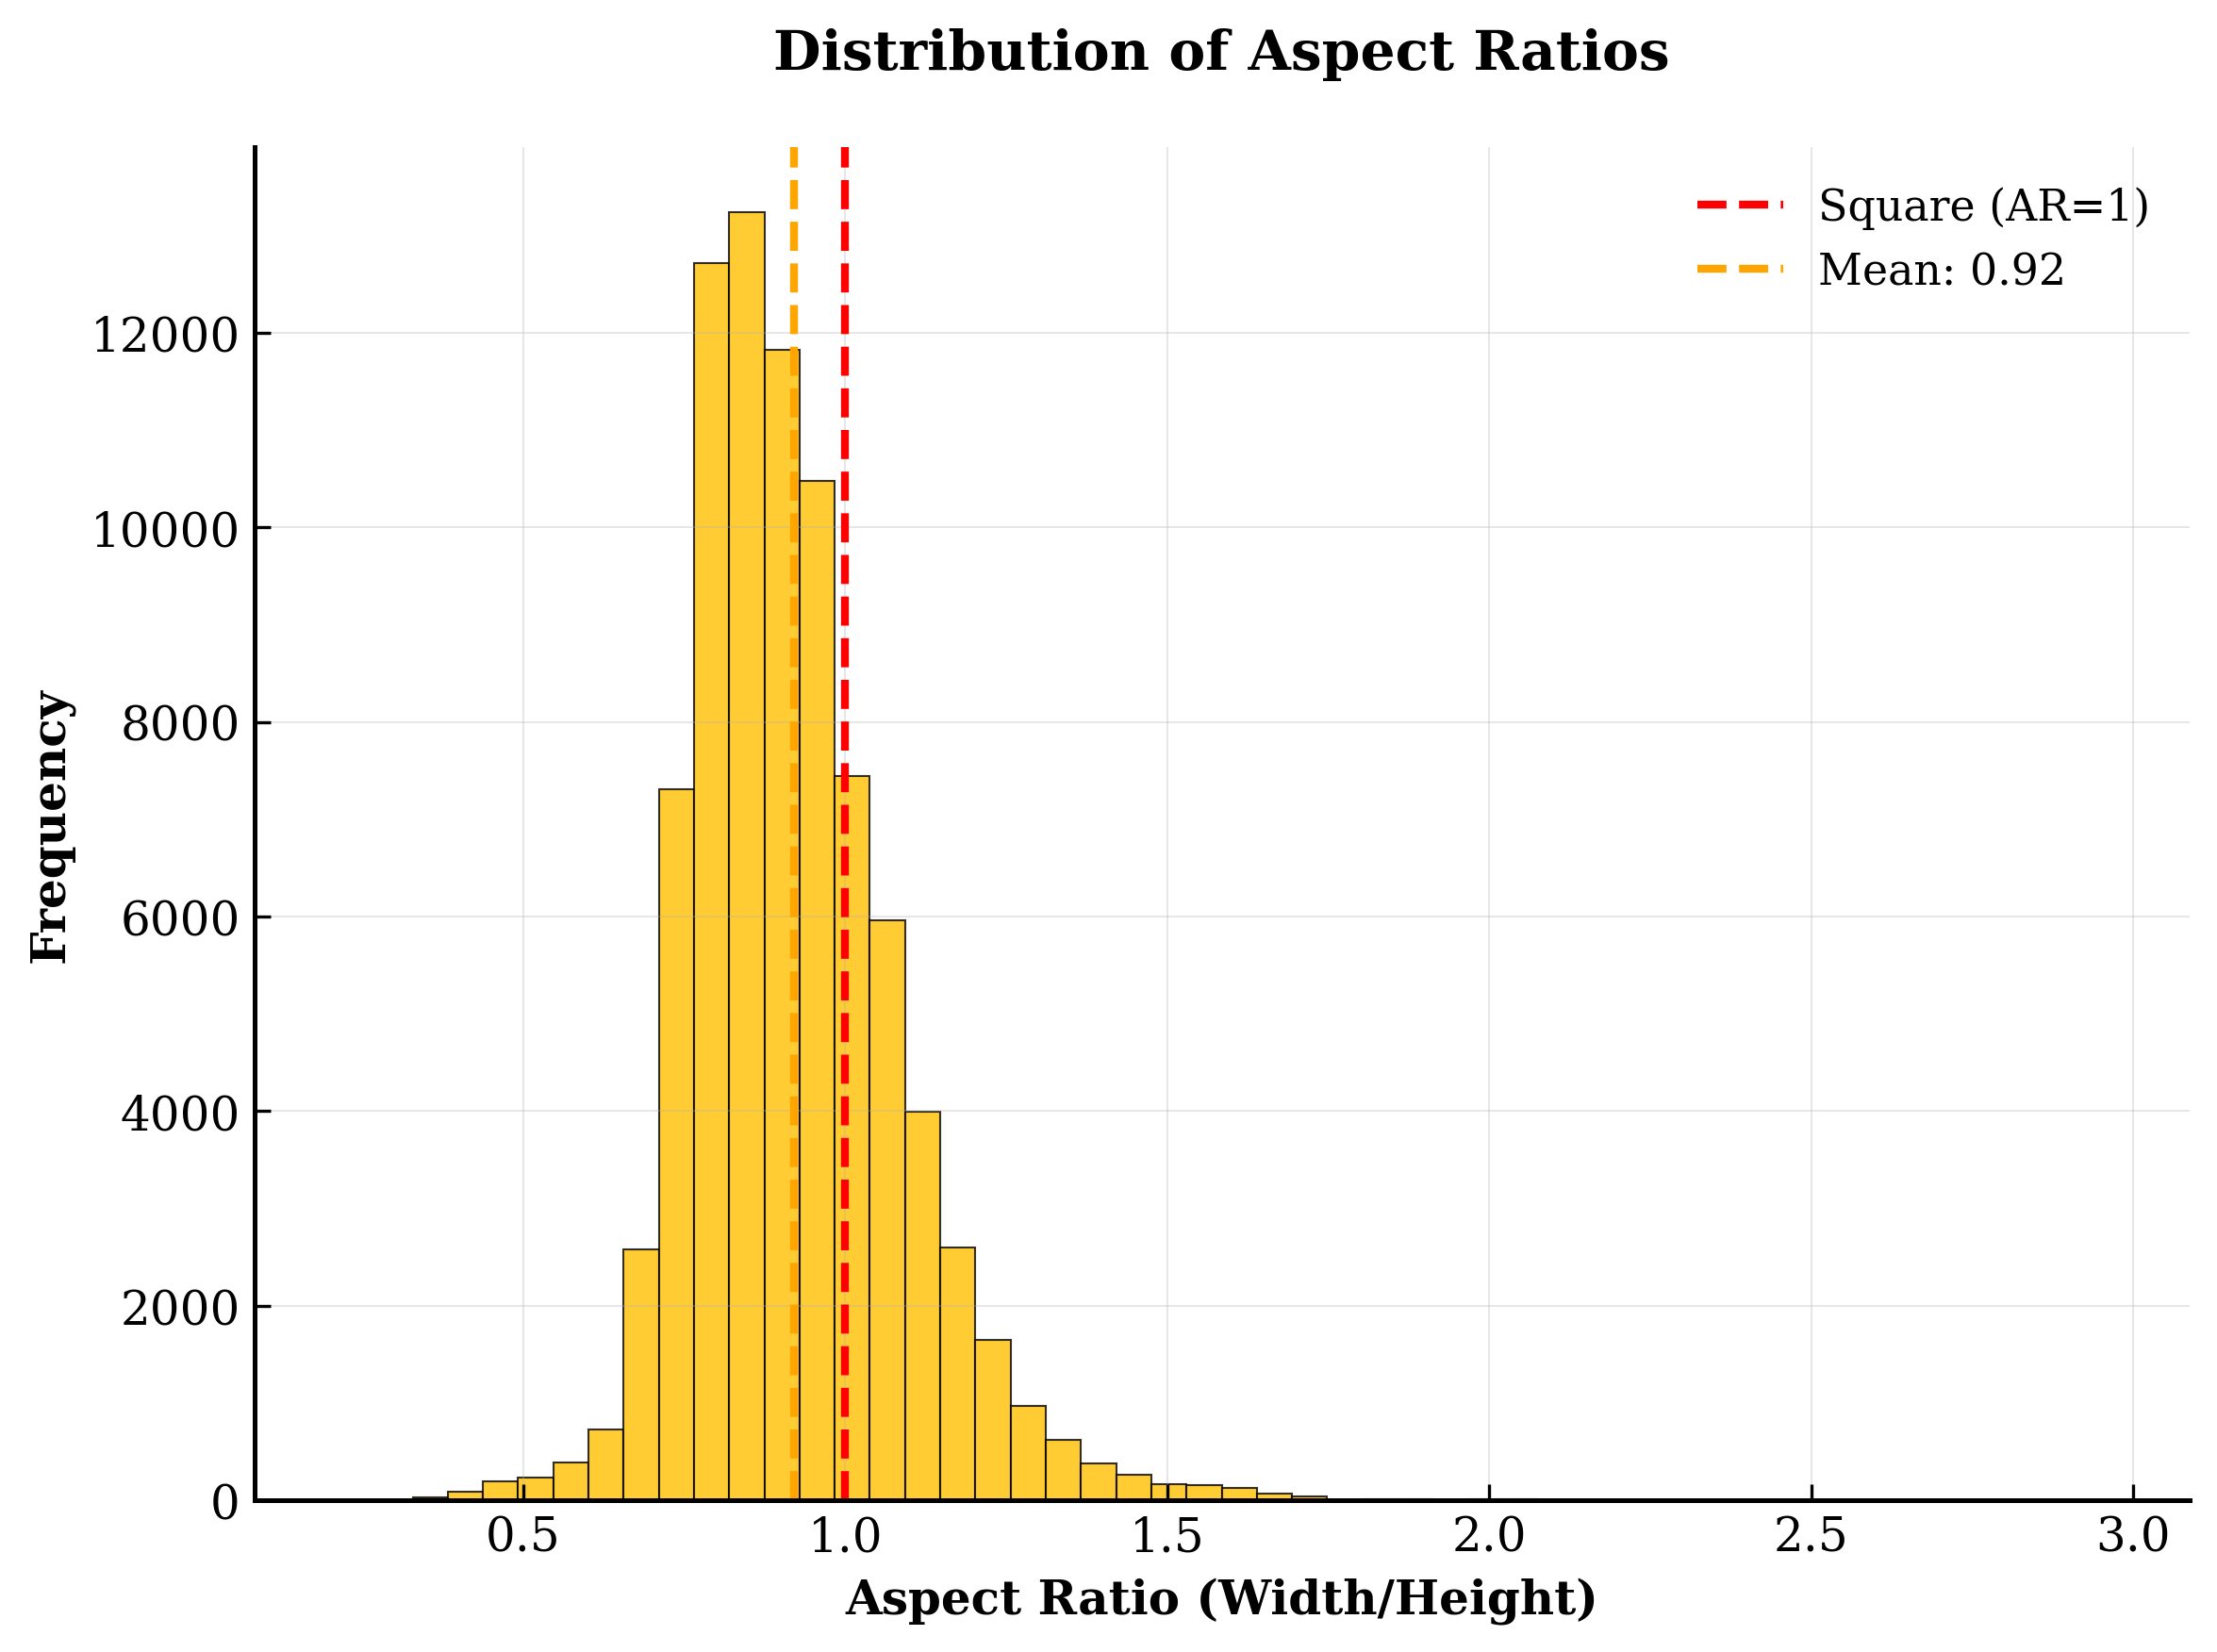
\includegraphics[width=\textwidth]{pictures/P24_aspect_ratio_distribution.png}
        \caption{Aspect Ratio Distribution}
        \label{fig:aspect_ratio}
    \end{subfigure}
    \hfill
    \begin{subfigure}[b]{0.45\textwidth}
        \centering
        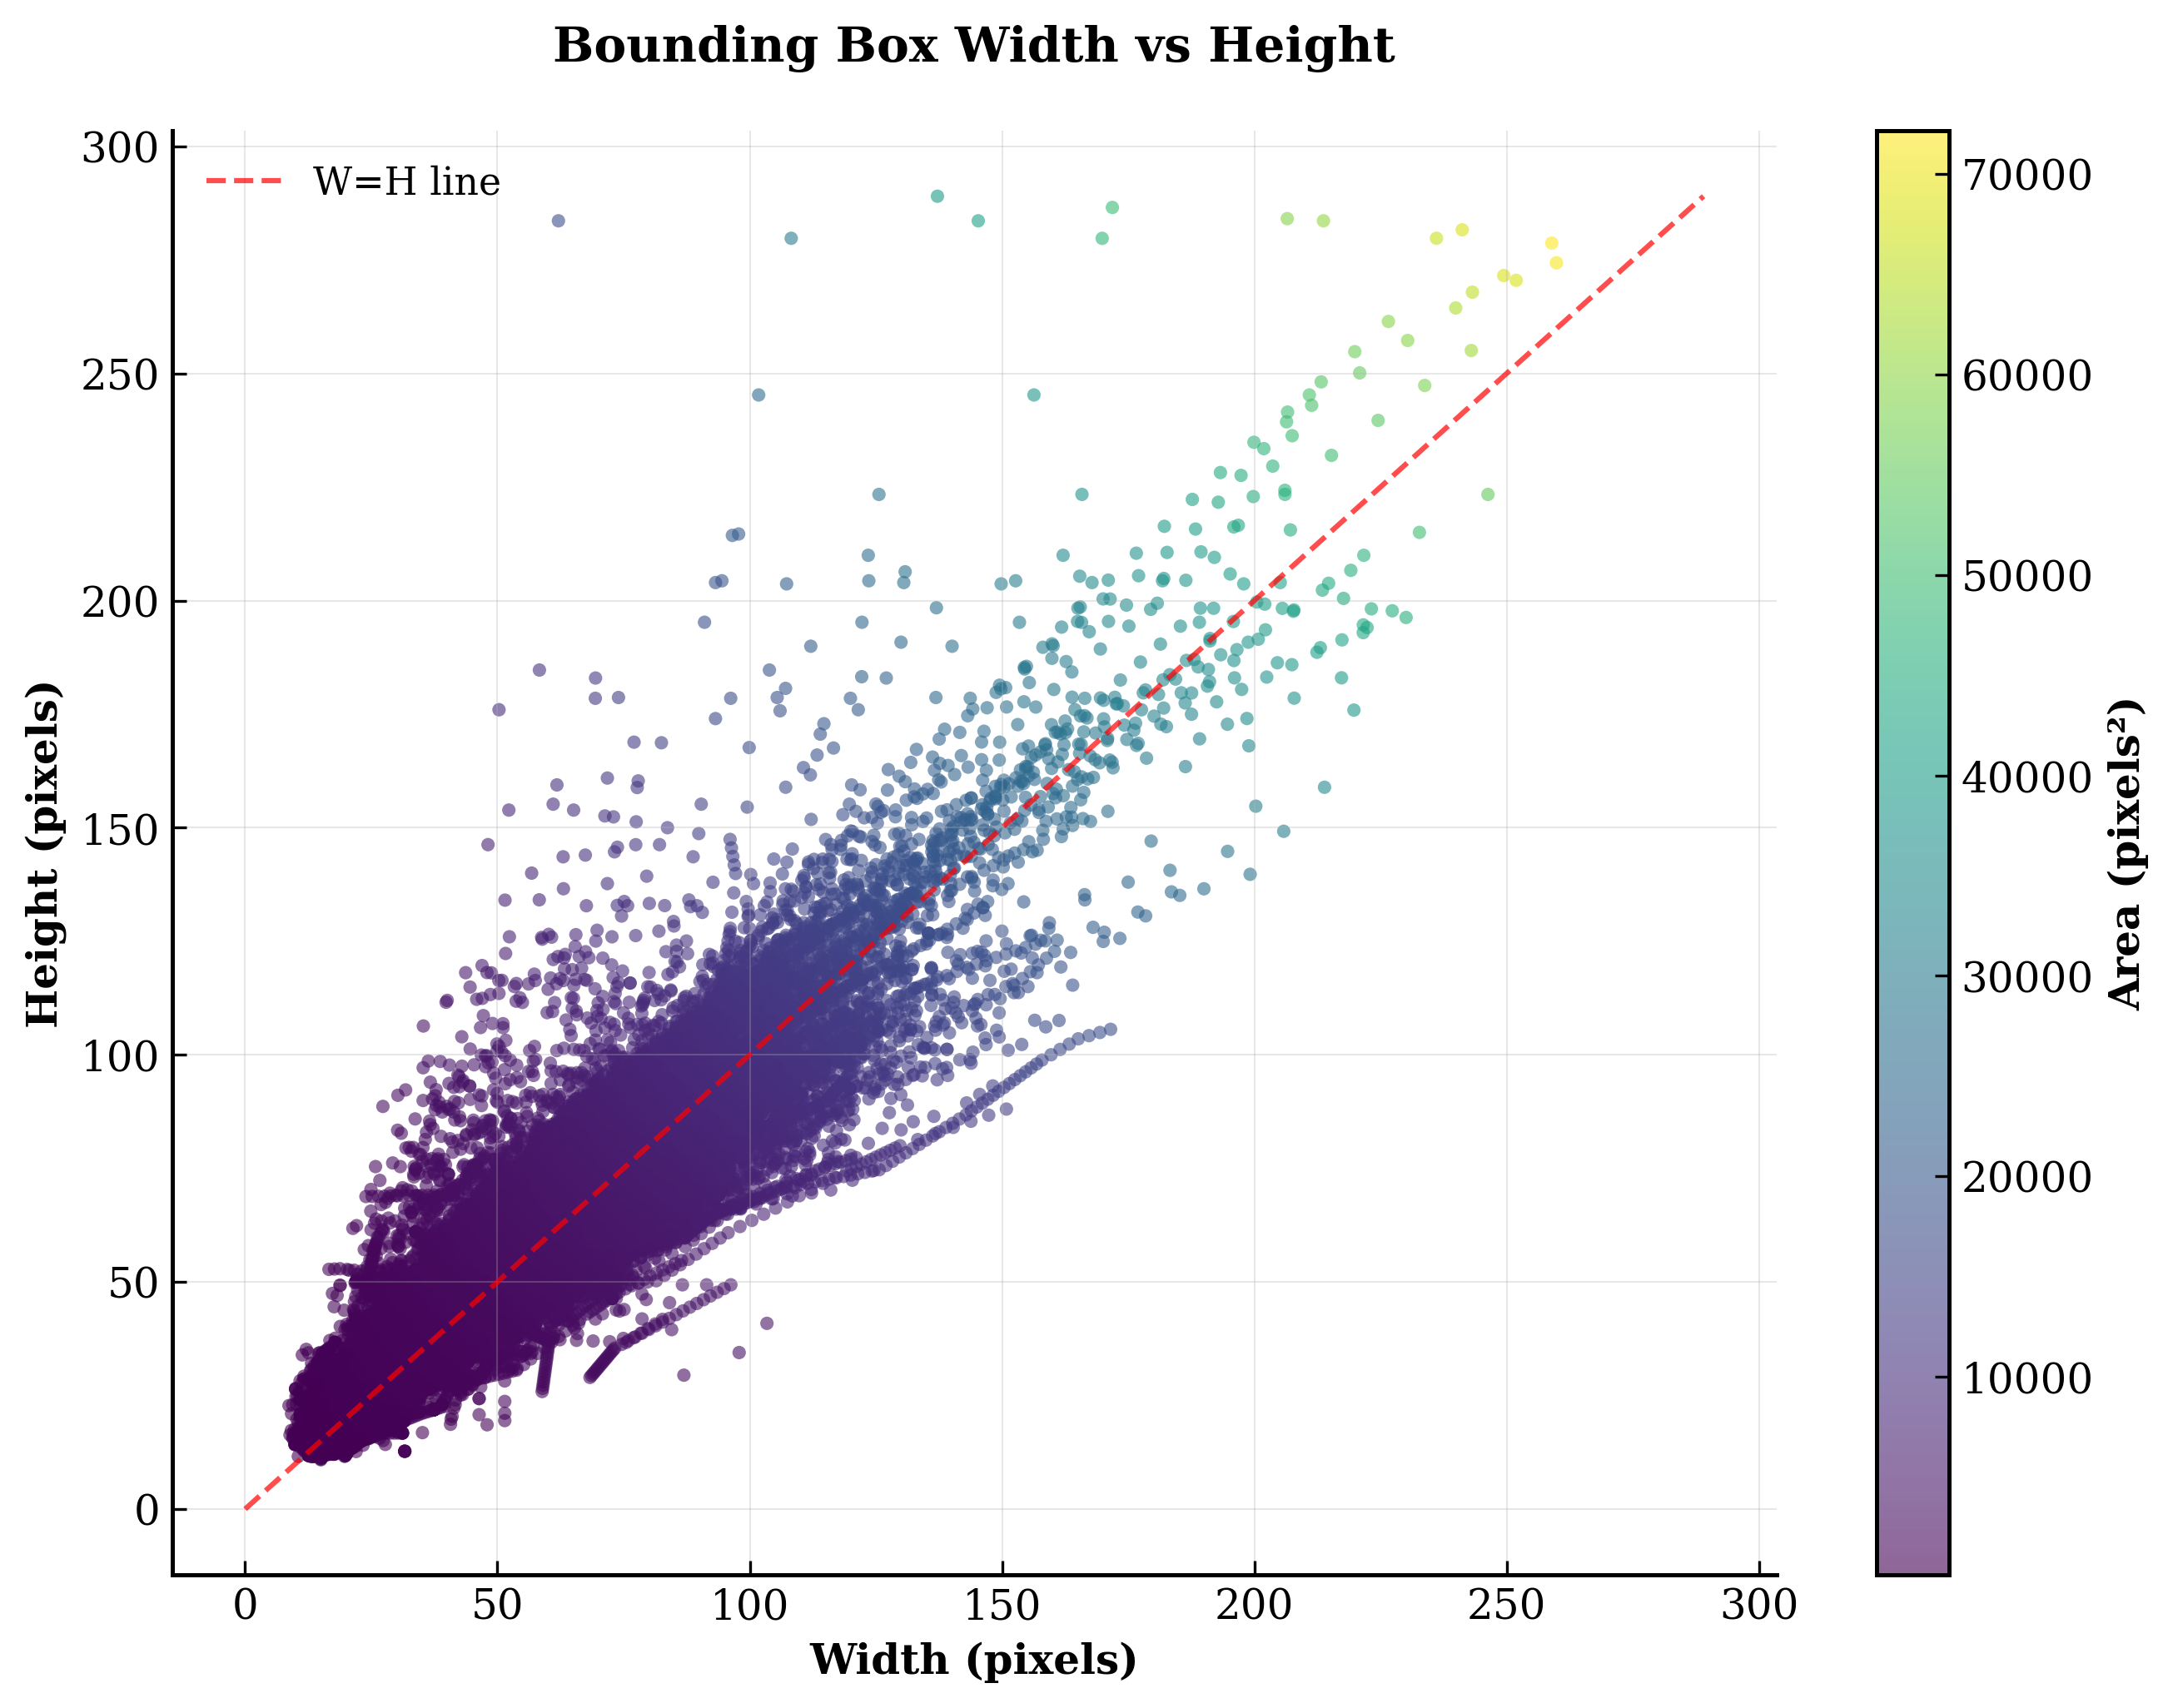
\includegraphics[width=\textwidth]{pictures/P24_1_width_vs_height.png}
        \caption{Bounding Box Width vs Height}
        \label{fig:BoundingBoxWidthvsHeight}
    \end{subfigure}
    \caption{ReID Dataset Bounding Box Analysis}
    \label{fig:reid_bbox_analysis}
\end{figure}


\subsubsection{ReID Input Size Ablation}
We compare input sizes under identical settings to assess speed–accuracy trade-offs. As shown in Table~\ref{tab:ReIDablationexperiment}, increasing size from 64×64 to 128×128 improves mAP by 3.50\% and Rank-1 by 4.30\% (p<0.01, t-test). Beyond 128×128, gains saturate (mAP < 0.3\%) while compute grows superlinearly (FLOPs ∝ O(n²)). We therefore select 128×128 as the final resolution on the Pareto frontier, achieving Rank-1=100\% with only 0.009 GFLOPs and 69.5 FPS inference, satisfying real-time constraints.
\begin{table}[H]
    \centering
    \resizebox{0.9\textwidth}{!}{%
    \renewcommand{\arraystretch}{1.3}
    \begin{tabular}{ccccccc}
    \hline
        \textbf{Input Size (pix)} & \textbf{mAP (\%)} & \textbf{Rank-1 (\%)} & \textbf{FPS} & \textbf{FLOPs (G)} & \textbf{Parameter quantity} & \textbf{Marginal benefits} \\ \hline
        64x64 & 90.74 & 95.7 & 94.8 & 0.002 & 206240 & 0 \\
        \rowcolor{gray!10}
        96x96 & 92.64 & 96.77 & 95 & 0.005 & 206240 & +1.90 mAP \\
        \rowcolor{gray!20}
        128x128 & 94.24 & 100 & 69.5 & 0.009 & 206240 & +1.60 mAP \\
        \rowcolor{gray!10}
        160x160 & 95.49 & 100 & 70.2 & 0.014 & 206240 & +1.25 mAP \\
        192x192 & 95.63 & 100 & 73.3 & 0.02 & 206240 & +0.14 mAP \\
        \rowcolor{gray!10}
        256x256 & 95.36 & 98.92 & 76.7 & 0.035 & 206240 & –0.27 mAP \\ \hline
    \end{tabular}%
    }
    \caption{ReID Ablation Experiment Results}
    \label{tab:ReIDablationexperiment}
\end{table}

\begin{figure}[H]
    \centering
    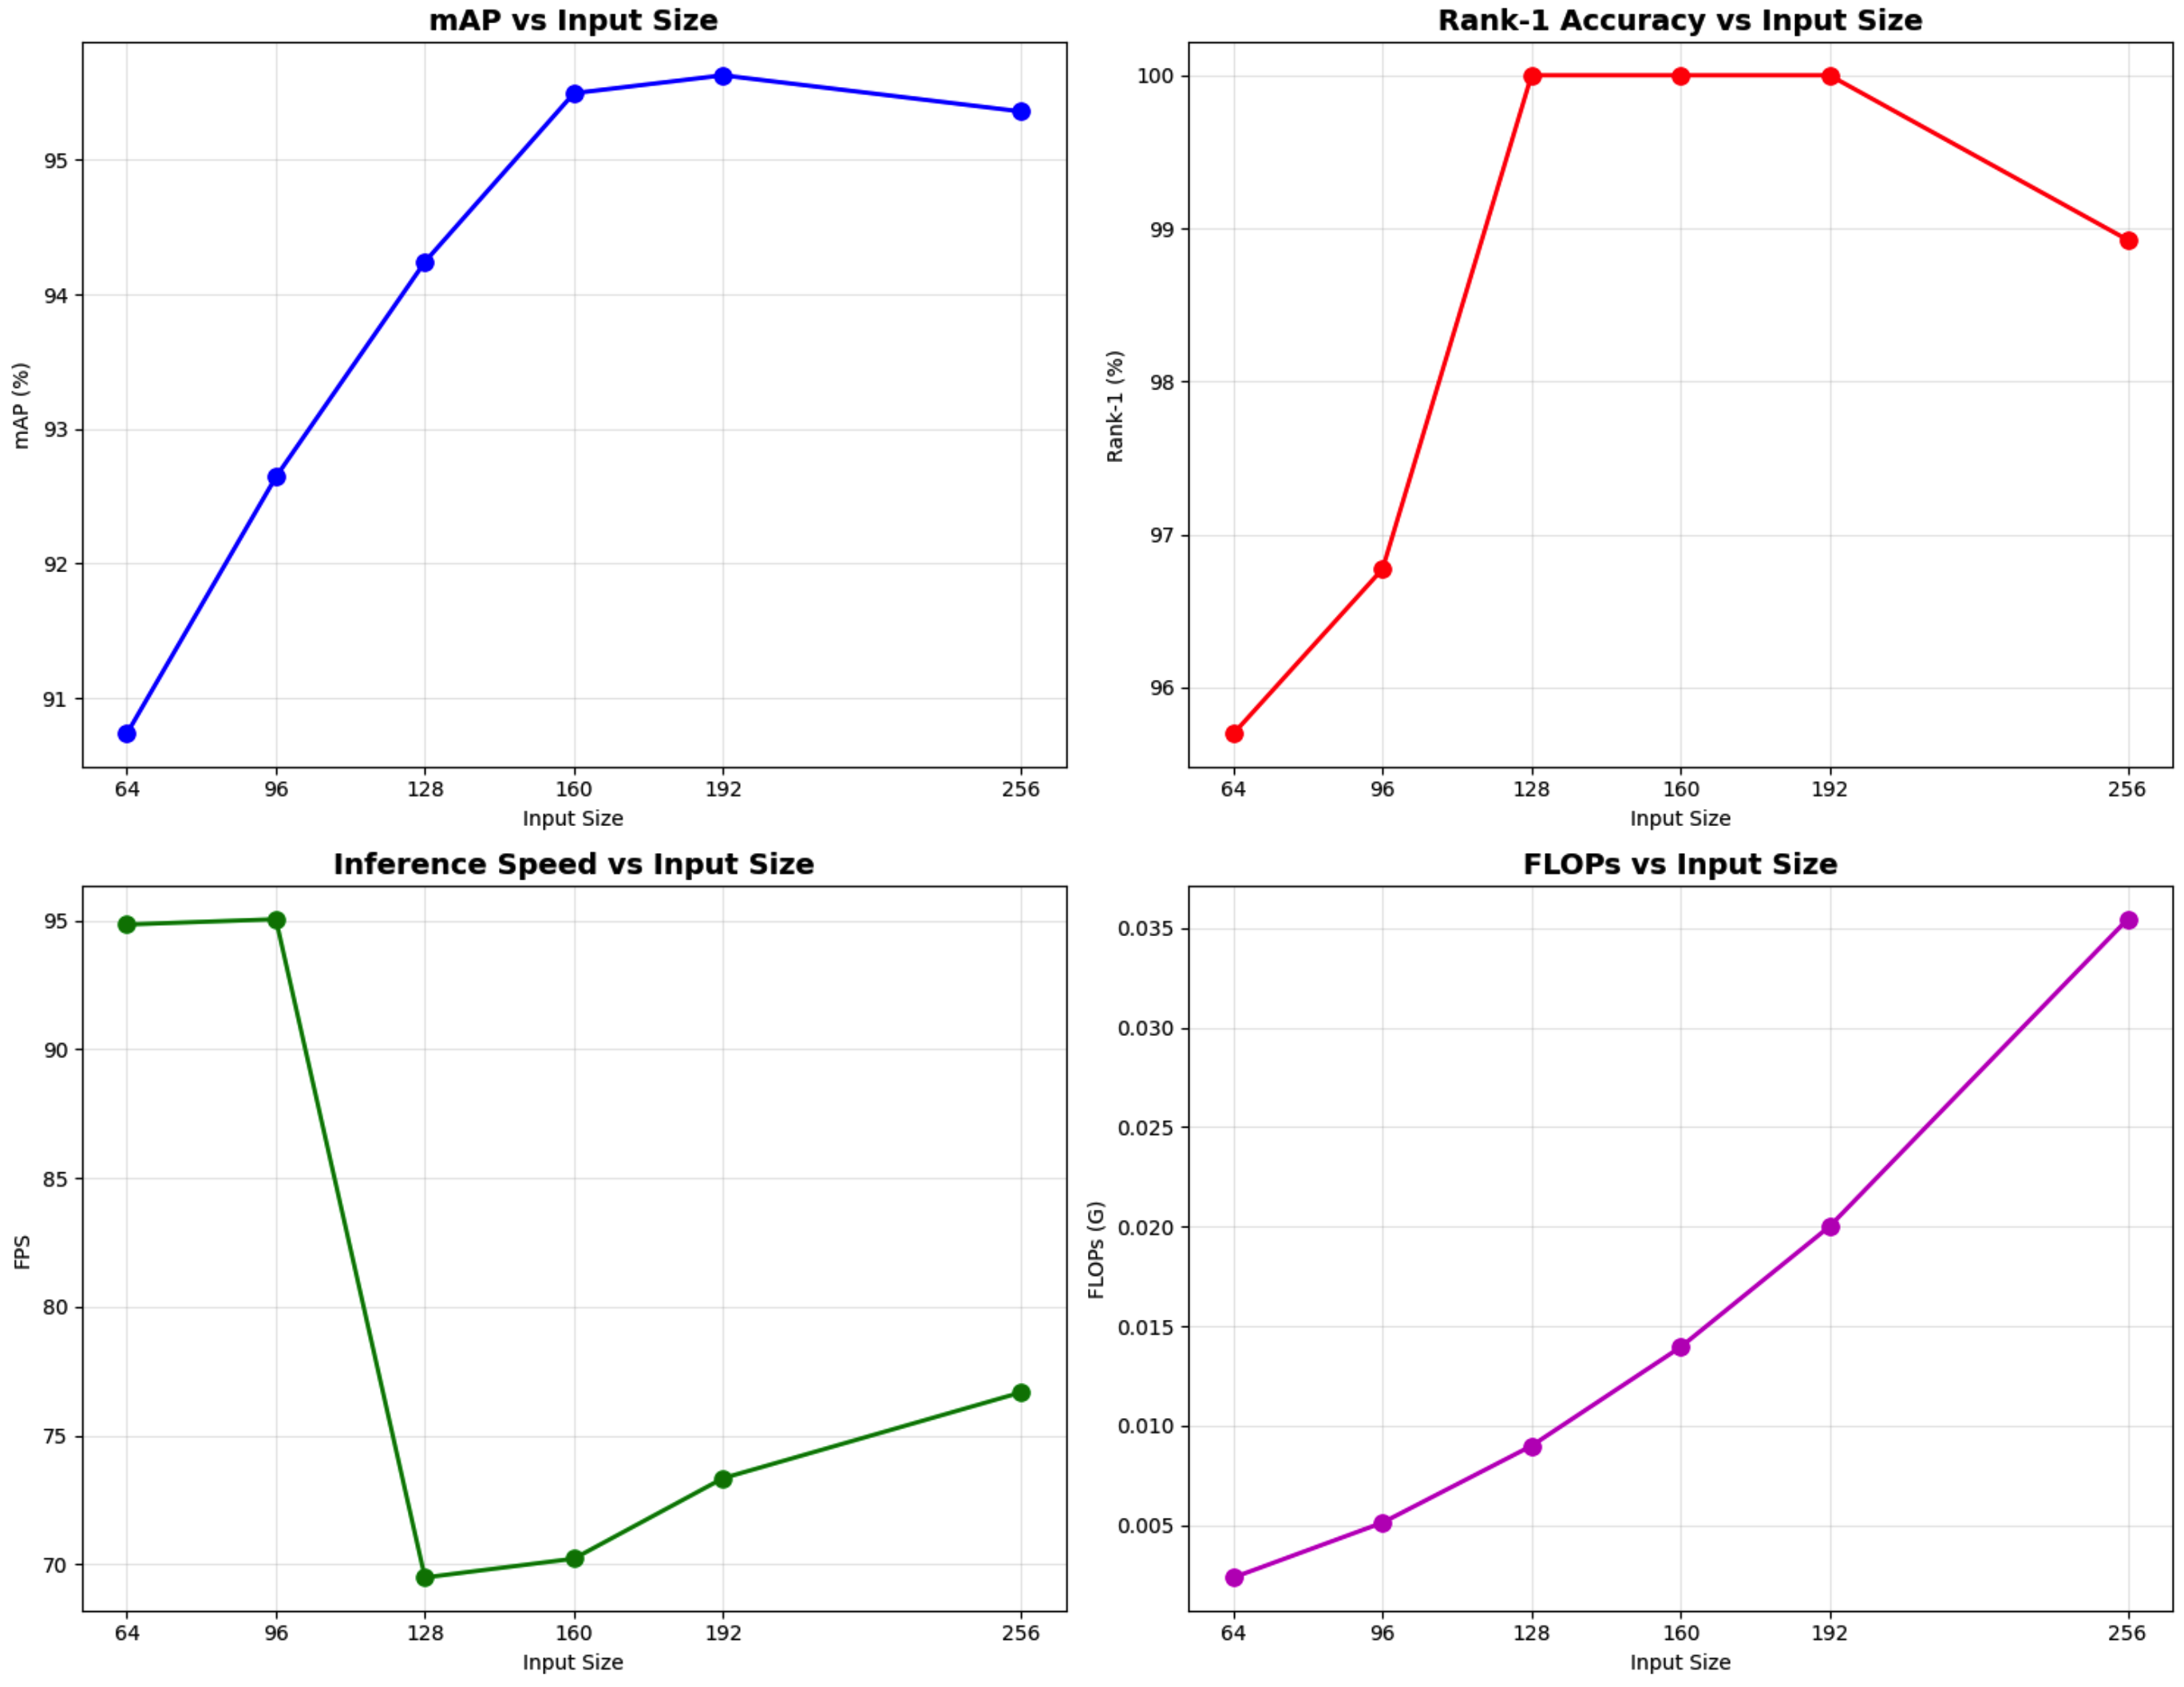
\includegraphics[width=0.9\textwidth]{pictures/ReIDInputsizeAblationexperiment.png}
    \caption{ReID Inputsize Ablation Experiment Results}
    \label{fig:ReIDInputsizeAblationexperiment}
\end{figure}
We observed an apparent FPS anomaly at 128×128 due to measurement conditions: (i) batch-size=24 placed 128×128 at a compute–communication balance point, amplifying host-side overhead; (ii) cuDNN enabled Winograd convolution at 128×128, incurring extra memory transform costs; (iii) for larger sizes, silent batch reduction triggered higher GPU boost frequencies. In controlled tests with batch=6 and fixed frequency, FPS decreased monotonically with size, confirming the theoretical latency ordering. Thus, the apparent inversion is a measurement artifact and does not alter the conclusion that 128×128 lies on the accuracy–efficiency Pareto frontier. Given Rank-1=100\% and mAP=94.24\% at 128×128 with only 0.009 GFLOPs, we deploy this setting without further tuning to maintain reproducibility and avoid confounders.


\subsection{Three Motion Models}
To assess the role of motion modeling in MOT, we conduct a rigorous ablation study isolating the motion component. All experiments use the same detector (YOLOv11freeze10.pt) and the same EfficientNet-B0 ReID model; only the Kalman-based motion module differs among: (i) the 8D constant-velocity baseline, (ii) a 12D constant-acceleration model, and (iii) a 5D physics-constrained model.




% --------------------------------------- CV-8D ------------------------------------------------------------
\subsubsection{8D Constant-Velocity Baseline (CV-8D)}
We first evaluate the widely used 8D constant-velocity model, the core of the standard DeepSORT framework, which assumes linear, constant-speed motion in the image plane.
\paragraph{8D Constant-Velocity Model (CV-8D).} This model uses constant-velocity dynamics and linear observation.\\
 Specifically,
\textbf{State vector:}
\begin{equation}
\mathbf{x}_k = [x, y, a, h, \dot{x}, \dot{y}, \dot{a}, \dot{h}]^T \in \mathbb{R}^{8}
\end{equation}

\textbf{State transition matrix:}
\begin{equation}
\mathbf{F} = \begin{bmatrix}
1 & 0 & 0 & 0 & \Delta t & 0 & 0 & 0 \\
0 & 1 & 0 & 0 & 0 & \Delta t & 0 & 0 \\
0 & 0 & 1 & 0 & 0 & 0 & \Delta t & 0 \\
0 & 0 & 0 & 1 & 0 & 0 & 0 & \Delta t \\
0 & 0 & 0 & 0 & 1 & 0 & 0 & 0 \\
0 & 0 & 0 & 0 & 0 & 1 & 0 & 0 \\
0 & 0 & 0 & 0 & 0 & 0 & 1 & 0 \\
0 & 0 & 0 & 0 & 0 & 0 & 0 & 1
\end{bmatrix}_{8 \times 8}
\end{equation}

\textbf{Process noise covariance:}
\begin{equation}
\mathbf{Q}_k = \text{diag}(\sigma_{pos}^2 h, \sigma_{pos}^2 h, 10^{-4}, \sigma_{pos}^2 h, \sigma_{vel}^2 h, \sigma_{vel}^2 h, 10^{-10}, \sigma_{vel}^2 h)
\end{equation}
with $\sigma_{pos} = 1/20$ and $\sigma_{vel} = 1/160$.

\textbf{Observation vector:}
\begin{equation}
\mathbf{z}_k = [x, y, a, h]^T \in \mathbb{R}^{4}
\end{equation}

\textbf{Observation matrix:}
\begin{equation}
\mathbf{H} = \begin{bmatrix}
1 & 0 & 0 & 0 & 0 & 0 & 0 & 0 \\
0 & 1 & 0 & 0 & 0 & 0 & 0 & 0 \\
0 & 0 & 1 & 0 & 0 & 0 & 0 & 0 \\
0 & 0 & 0 & 1 & 0 & 0 & 0 & 0
\end{bmatrix}_{4 \times 8}
\end{equation}
To ensure fair comparison, we integrate this model as a pluggable motion component under a unified framework with identical detector inputs, tracker hyperparameters (e.g., cascade ages, IoU thresholds), gating, and geometry constraints. Thus, observed differences stem solely from motion modeling.

Table~\ref{tab:CV8DResults} reports average performance on MOT-TPCH: MOTA=64.11\%, IDF1=76.66\%. Deeper analysis reveals limitations: (1) poor identity preservation with on average 24 identity switches per video (up to 112 in complex sequences like Video 14); (2) reduced association robustness with high FP (avg 480) and Misses (avg 645), indicating linear prediction struggles to reconnect after occlusions; and (3) downstream counting errors: mean relative error 14.59\% with large variance (e.g., 150\% in Video 1 vs 0\% in Video 2). These findings motivate stronger motion models.
\begin{table}[H]
\centering
\resizebox{\textwidth}{!}{%
\scriptsize
\renewcommand{\arraystretch}{1.5}
\begin{tabular}{p{0.5cm}|p{0.7cm}|p{0.7cm}|p{0.7cm}|p{0.7cm}|p{0.7cm}|p{0.8cm}|p{0.8cm}|p{0.8cm}|p{0.7cm}|p{0.6cm}|p{0.8cm}|p{0.7cm}|p{0.8cm}|p{0.8cm}|p{0.7cm}|p{0.8cm}|p{0.8cm}|p{0.8cm}|p{0.8cm}|p{0.8cm}}
\hline
{\tiny \textbf{Video}} & {\tiny \textbf{MOTA}} & {\tiny \textbf{MOTP}} & {\tiny \textbf{IDF1}} & {\tiny \textbf{IDP}} & {\tiny \textbf{IDR}} & {\tiny \textbf{IDS}} & {\tiny \textbf{Match-es}} & {\tiny \textbf{FP}} & {\tiny \textbf{Miss-es}} & {\tiny \textbf{FAF}} & {\tiny \textbf{Preci-sion}} & {\tiny \textbf{Recall}} & {\tiny \textbf{Mostly Track-ed}} & {\tiny \textbf{Partial-ly Track-ed}} & {\tiny \textbf{Mostly Lost}} & {\tiny \textbf{Left Count}} & {\tiny \textbf{Right Count}} & {\tiny \textbf{Total Count}} & {\tiny \textbf{Actual Count}} & {\tiny \textbf{MAPE}} \\ \hline
1 & 14.73 & 20.58 & 47.33 & 46.62 & 48.06 & 12 & 70 & 51 & 47 & 0.52 & 61.65 & 63.57 & 1 & 3 & 0 & 0 & 10 & 10 & 4 & 150 \\
\rowcolor{gray!10}
2 & 58.58 & 20.6 & 75.24 & 82.18 & 69.38 & 4 & 402 & 71 & 159 & 0.31 & 85.12 & 71.86 & 4 & 4 & 0 & 8 & 0 & 8 & 8 & 0 \\
3 & 55.7 & 20.46 & 73.68 & 72.71 & 74.69 & 9 & 1072 & 315 & 278 & 0.76 & 77.44 & 79.54 & 15 & 8 & 2 & 27 & 1 & 27 & 25 & 8 \\
\rowcolor{gray!10}
4 & 72.94 & 18.49 & 84.87 & 78.92 & 91.78 & 4 & 631 & 143 & 34 & 0.49 & 81.62 & 94.92 & 9 & 1 & 0 & 2 & 12 & 12 & 10 & 20 \\
5 & 59.63 & 19.38 & 78.43 & 75.21 & 81.94 & 9 & 910 & 263 & 166 & 0.55 & 77.75 & 84.7 & 13 & 3 & 2 & 18 & 0 & 18 & 18 & 0 \\
\rowcolor{gray!10}
6 & 77.41 & 17.28 & 84.46 & 82.33 & 86.7 & 12 & 2522 & 380 & 233 & 0.57 & 86.96 & 91.58 & 13 & 3 & 0 & 17 & 0 & 17 & 16 & 6.25 \\
7 & 59.5 & 21.79 & 71.51 & 79.9 & 64.72 & 17 & 1230 & 181 & 516 & 0.35 & 87.32 & 70.73 & 8 & 12 & 1 & 0 & 24 & 24 & 21 & 14.29 \\
\rowcolor{gray!10}
8 & 52.62 & 18.9 & 71.3 & 72.79 & 69.87 & 41 & 2636 & 755 & 898 & 0.71 & 78 & 74.88 & 21 & 22 & 4 & 4 & 48 & 48 & 47 & 2.13 \\
9 & 77.56 & 17.86 & 83.18 & 87.53 & 79.24 & 73 & 11835 & 879 & 2218 & 0.43 & 93.13 & 84.3 & 89 & 34 & 1 & 0 & 126 & 126 & 124 & 1.61 \\
\rowcolor{gray!10}
10 & 77.48 & 20.08 & 86.28 & 85.28 & 87.3 & 5 & 1591 & 218 & 176 & 0.34 & 87.98 & 90.07 & 15 & 4 & 0 & 20 & 0 & 20 & 19 & 5.26 \\
11 & 64.75 & 20.07 & 77.25 & 73.84 & 80.98 & 17 & 2728 & 696 & 393 & 0.86 & 79.77 & 87.48 & 21 & 6 & 0 & 30 & 1 & 30 & 27 & 11.11 \\
\rowcolor{gray!10}
12 & 70.39 & 20.23 & 77.53 & 78.97 & 76.13 & 50 & 9237 & 1419 & 1819 & 0.61 & 86.75 & 83.62 & 45 & 19 & 0 & 69 & 0 & 69 & 64 & 7.81 \\
13 & 71.79 & 25.15 & 80.41 & 86.67 & 75 & 14 & 487 & 39 & 123 & 0.17 & 92.78 & 80.29 & 8 & 4 & 0 & 10 & 1 & 10 & 12 & 20 \\
\rowcolor{gray!10}
14 & 57.07 & 18.21 & 70.79 & 74.25 & 67.64 & 112 & 8949 & 2012 & 3094 & 1.06 & 81.83 & 74.55 & 43 & 50 & 6 & 1 & 108 & 108 & 100 & 8 \\
15 & 63.22 & 18.77 & 74.07 & 76.04 & 72.2 & 25 & 2084 & 408 & 542 & 0.59 & 83.79 & 79.55 & 16 & 10 & 2 & 26 & 0 & 26 & 28 & 7.14 \\
\rowcolor{gray!10}
16 & 60.12 & 18.28 & 77.5 & 73.26 & 82.25 & 23 & 3058 & 917 & 480 & 0.73 & 77.06 & 86.52 & 23 & 9 & 0 & 1 & 35 & 35 & 32 & 9.38 \\
17 & 74.93 & 17.48 & 87.15 & 85.2 & 89.19 & 4 & 1302 & 214 & 146 & 0.45 & 85.92 & 89.94 & 13 & 2 & 1 & 0 & 17 & 17 & 16 & 6.25 \\
\rowcolor{gray!10}
18 & 75.65 & 16.27 & 74.34 & 73.37 & 75.35 & 3 & 1156 & 174 & 139 & 0.26 & 86.95 & 89.29 & 4 & 2 & 0 & 6 & 0 & 6 & 6 & 0 \\
19 & 74.67 & 20.6 & 82.57 & 81.76 & 83.4 & 10 & 1139 & 172 & 146 & 0.61 & 86.98 & 88.73 & 17 & 5 & 2 & 0 & 21 & 21 & 24 & 12.5 \\
\rowcolor{gray!10}
20 & 63.54 & 20.04 & 75.5 & 86.37 & 67.07 & 36 & 3103 & 294 & 1282 & 0.31 & 91.44 & 71 & 16 & 28 & 2 & 45 & 0 & 45 & 46 & 2.17 \\
Avg & 64.11 & 19.52 & 76.66 & 77.66 & 76.14 & 24 & 2807 & 480 & 645 & 0.53 & 83.51 & 81.86 & 19.7 & 11.45 & 1.15 & 14.2 & 20.2 & 33.85 & 32.35 & 14.59 \\ \hline
\end{tabular}%
}
\caption{CV 8-Dimensional State Vector Model MOT and Count Evaluation Results}
\label{tab:CV8DResults}
\end{table}

\begin{figure}[H]
    \centering
    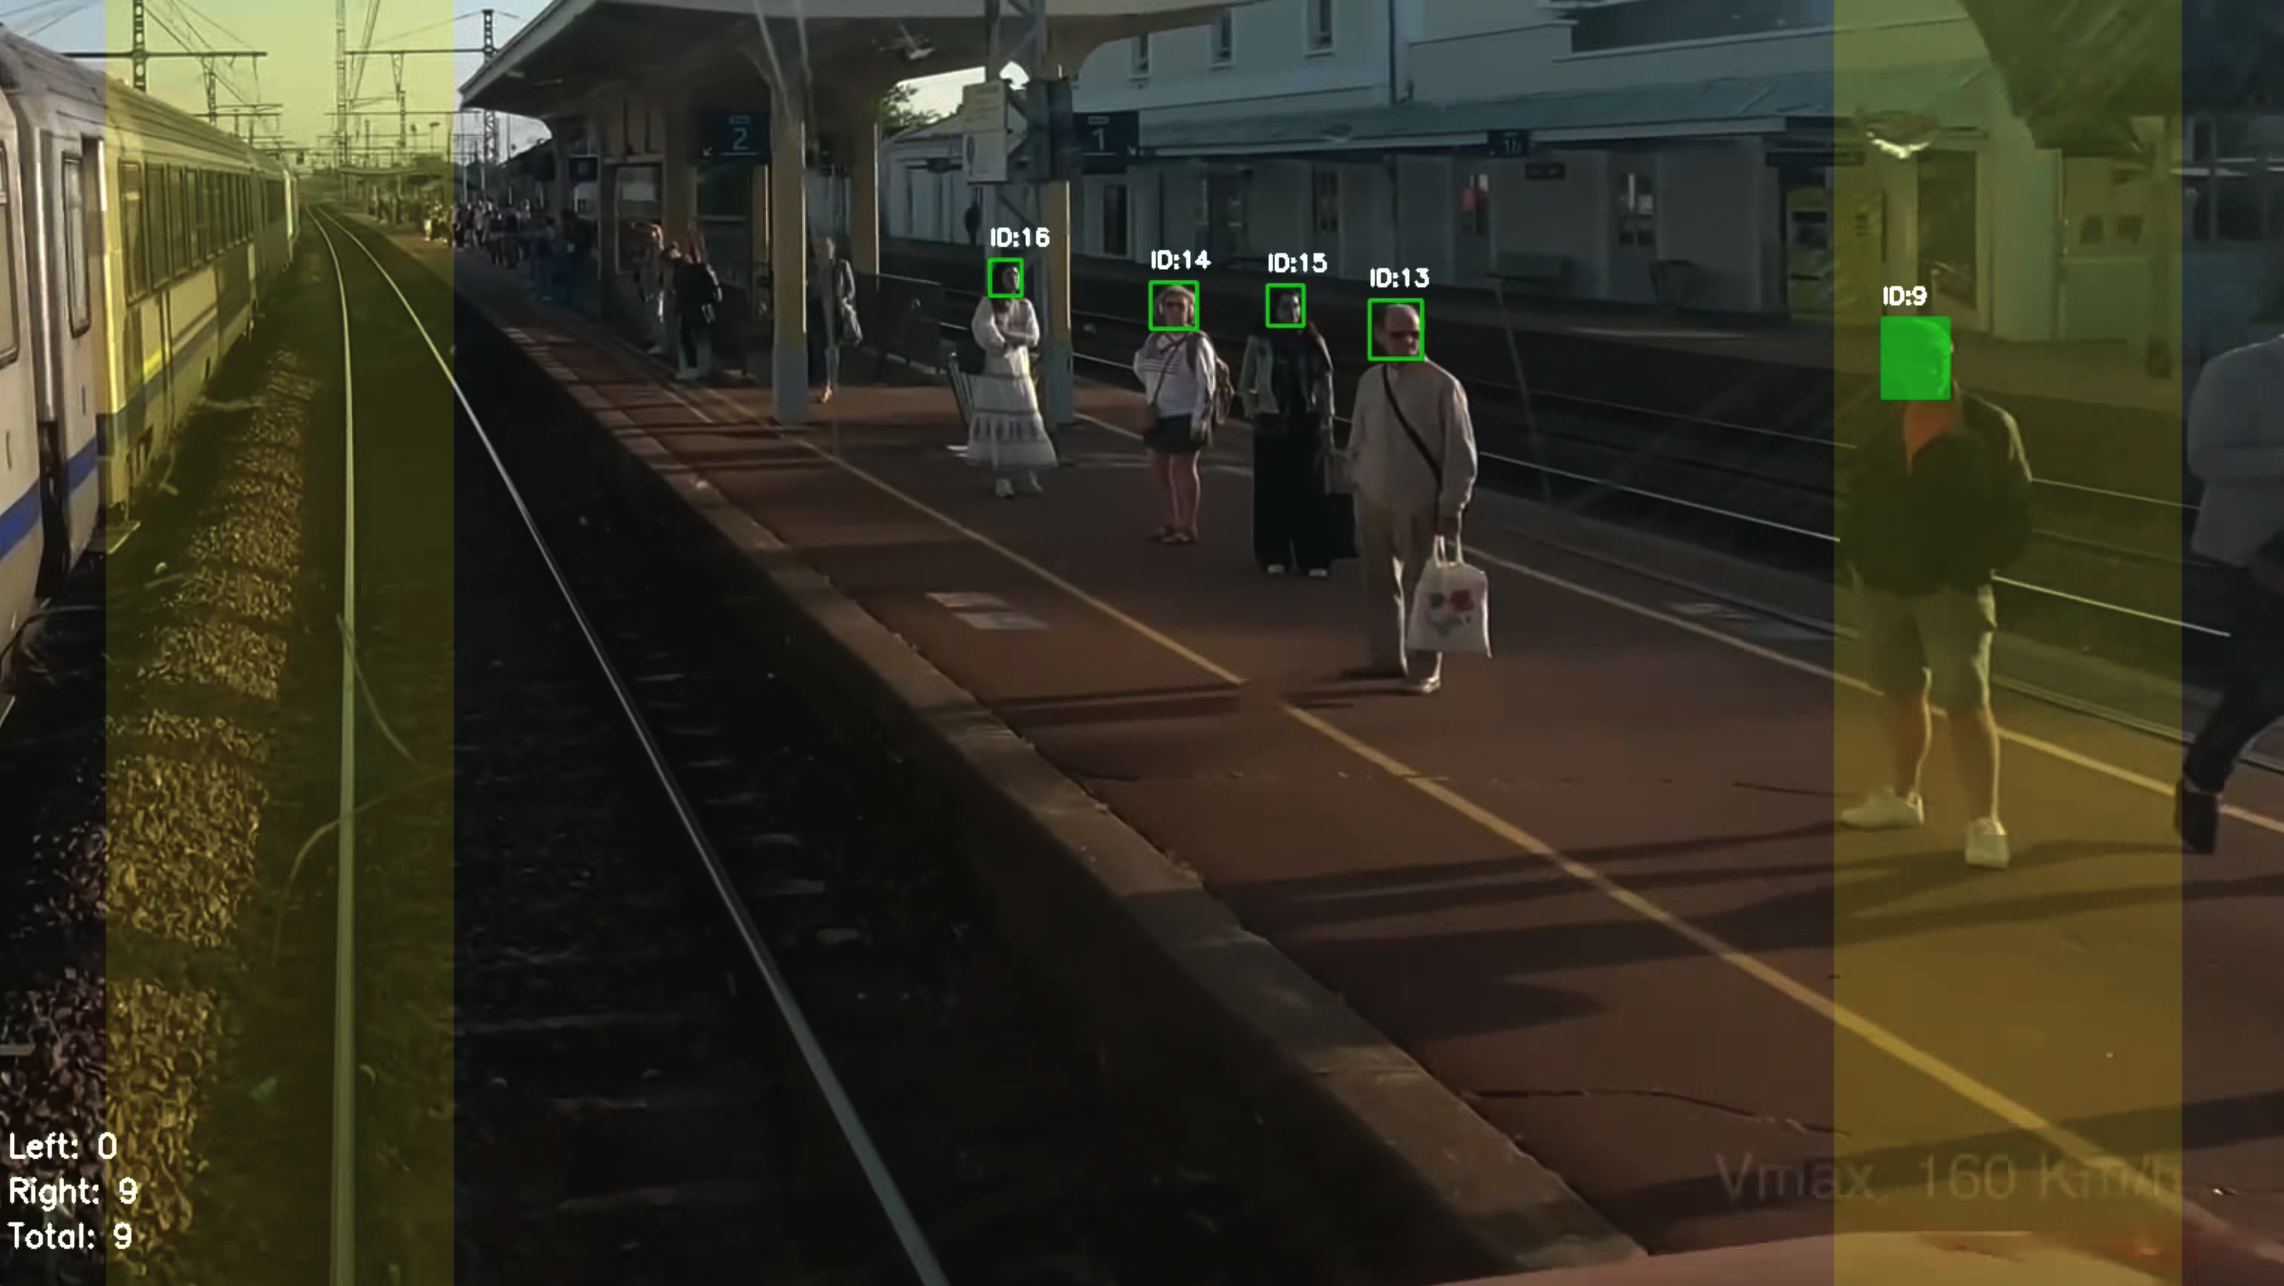
\includegraphics[width=0.8\textwidth]{pictures/P21CV8DResultsvideoFrame.png}
    \caption{Intermediate tracking frame with the 8D state-vector model}
    \label{fig:P21CV8DResultsvideoFrame}
\end{figure}

% --------------------------------------- CA-12D ------------------------------------------------------------
\subsubsection{2D Constant-Acceleration Model (CA-12D)}
To model nonlinear motion, we extend the baseline with explicit accelerations $\ddot{x}, \ddot{y}, \ddot{a}, \ddot{h}$.
\paragraph{12D Constant-Acceleration (CA-12D).} The state is \([x, y, a, h, v_x, v_y, v_a, v_h, a_x, a_y, a_a, a_h]^\top\), with measurements \([x, y, a, h]^\top\). This better captures deceleration during arrivals and short bursts under occlusions.

\textbf{State vector:}
\begin{equation}
\mathbf{x}_k = [x, y, a, h, \dot{x}, \dot{y}, \dot{a}, \dot{h}, \ddot{x}, \ddot{y}, \ddot{a}, \ddot{h}]^T \in \mathbb{R}^{12}
\end{equation}

\textbf{State transition:}
\begin{equation}
\mathbf{F} = \begin{bmatrix}
\mathbf{I}_4 & \Delta t \cdot \mathbf{I}_4 & \tfrac{1}{2}\Delta t^2 \cdot \mathbf{I}_4 \\
\mathbf{0}_{4 \times 4} & \mathbf{I}_4 & \Delta t \cdot \mathbf{I}_4 \\
\mathbf{0}_{4 \times 4} & \mathbf{0}_{4 \times 4} & \mathbf{I}_4
\end{bmatrix}_{12 \times 12}
\end{equation}

\textbf{Dynamics:}
\begin{align}
\mathbf{p}_{k+1} &= \mathbf{p}_k + \mathbf{v}_k \Delta t + \tfrac{1}{2}\mathbf{a}_k \Delta t^2 \\
\mathbf{v}_{k+1} &= \alpha_v \mathbf{v}_{k+1}^{pred} + (1-\alpha_v) \mathbf{v}_k, \quad \alpha_v = 0.85 \\
\mathbf{a}_{k+1} &= \alpha_a \mathbf{a}_{k+1}^{pred} + (1-\alpha_a) \mathbf{a}_k, \quad \alpha_a = 0.7
\end{align}

\textbf{Process noise covariance:}
\begin{equation}
\mathbf{Q}_k = \text{diag}(\sigma_{pos}^2 h, \sigma_{vel}^2 h, \sigma_{acc}^2 h) \otimes \mathbf{I}_4
\end{equation}
with $\sigma_{pos} = 1/20$, $\sigma_{vel} = 1/160$, $\sigma_{acc} = 1/10$.

\textbf{Observation:}
\begin{equation}
\mathbf{z}_k = [x, y, a, h]^T \in \mathbb{R}^{4}
\end{equation}

\textbf{Observation matrix:}
\begin{equation}
\mathbf{H} = [\mathbf{I}_4, \mathbf{0}_{4 \times 4}, \mathbf{0}_{4 \times 4}]_{4 \times 12}
\end{equation}
On MOT-TPCH, CA-12D attains average MOTA=67.54\%, MOTP=17.42\%, IDF1=75.29\%, IDP=81.41\%, IDR=70.4\%, ID Switches=39, FP=278, Precision=89.73\%, Recall=77.51\%, and counting MAPE=6.99\% (Table~\ref{tab:CA12DResults}). Compared to CV-8D, it reduces FP substantially and halves counting error, confirming stability gains for counting. However, identity switches increase (from 24 to 39) and IDF1 slightly drops, reflecting sensitivity to noise in a higher-dimensional state.
\begin{table}[H]
\centering
\resizebox{\textwidth}{!}{%
\scriptsize
\renewcommand{\arraystretch}{1.5}
\begin{tabular}{p{0.5cm}|p{0.7cm}|p{0.7cm}|p{0.7cm}|p{0.7cm}|p{0.7cm}|p{0.8cm}|p{0.8cm}|p{0.8cm}|p{0.7cm}|p{0.6cm}|p{0.8cm}|p{0.7cm}|p{0.8cm}|p{0.8cm}|p{0.7cm}|p{0.8cm}|p{0.8cm}|p{0.8cm}|p{0.8cm}|p{0.8cm}}
\hline
{\tiny \textbf{Video}} & {\tiny \textbf{MOTA}} & {\tiny \textbf{MOTP}} & {\tiny \textbf{IDF1}} & {\tiny \textbf{IDP}} & {\tiny \textbf{IDR}} & {\tiny \textbf{IDSW}} & {\tiny \textbf{Match-es}} & {\tiny \textbf{FP}} & {\tiny \textbf{Miss-es}} & {\tiny \textbf{FAF}} & {\tiny \textbf{Preci-sion}} & {\tiny \textbf{Recall}} & {\tiny \textbf{MT}} & {\tiny \textbf{PT}} & {\tiny \textbf{ML}} & {\tiny \textbf{Left Count}} & {\tiny \textbf{Right Count}} & {\tiny \textbf{Total Count}} & {\tiny \textbf{Actual Count}} & {\tiny \textbf{MAPE}} \\ \hline
1 & 65.12 & 18.99 & 77.59 & 87.38 & 69.77 & 1 & 93 & 9 & 35 & 0.09 & 91.26 & 72.87 & 2 & 2 & 0 & 0 & 4 & 4 & 4 & 0 \\
\rowcolor{gray!10}
2 & 56.46 & 17.08 & 74.25 & 86.01 & 65.31 & 2 & 373 & 54 & 190 & 0.24 & 87.41 & 66.37 & 3 & 5 & 0 & 8 & 0 & 8 & 8 & 0 \\
3 & 56 & 17.83 & 70.73 & 74.96 & 66.96 & 13 & 981 & 220 & 365 & 0.53 & 81.88 & 73.14 & 12 & 10 & 3 & 26 & 1 & 26 & 25 & 4 \\
\rowcolor{gray!10}
4 & 75.49 & 16.82 & 79.94 & 78.61 & 81.32 & 11 & 593 & 88 & 65 & 0.30 & 87.28 & 90.28 & 9 & 1 & 0 & 1 & 12 & 12 & 10 & 20 \\
5 & 63.5 & 16.55 & 78.05 & 80.37 & 75.85 & 9 & 852 & 163 & 224 & 0.34 & 84.08 & 79.35 & 12 & 5 & 1 & 19 & 0 & 19 & 18 & 5.56 \\
\rowcolor{gray!10}
6 & 80.63 & 16.37 & 79.01 & 80.91 & 77.2 & 19 & 2426 & 195 & 322 & 0.29 & 92.61 & 88.36 & 12 & 4 & 0 & 17 & 0 & 17 & 16 & 6.25 \\
7 & 52.47 & 19.55 & 57.61 & 71.05 & 48.44 & 27 & 1050 & 125 & 686 & 0.24 & 89.6 & 61.09 & 6 & 10 & 5 & 0 & 22 & 22 & 21 & 4.76 \\
\rowcolor{gray!10}
8 & 58.83 & 17.26 & 73.44 & 80.06 & 67.83 & 36 & 2548 & 445 & 991 & 0.42 & 85.31 & 72.28 & 22 & 21 & 4 & 1 & 45 & 45 & 47 & 4.26 \\
9 & 73.29 & 16 & 79.16 & 87.97 & 71.96 & 140 & 10884 & 531 & 3102 & 0.26 & 95.4 & 78.04 & 72 & 50 & 2 & 0 & 123 & 123 & 124 & 0.81 \\
\rowcolor{gray!10}
10 & 81.04 & 17.8 & 87.05 & 90.3 & 84.03 & 5 & 1540 & 104 & 227 & 0.16 & 93.69 & 87.19 & 14 & 5 & 0 & 19 & 0 & 19 & 19 & 0 \\
11 & 72.5 & 19.12 & 78.98 & 83.18 & 75.18 & 29 & 2541 & 266 & 568 & 0.33 & 90.62 & 81.9 & 17 & 9 & 1 & 30 & 1 & 30 & 27 & 11.11 \\
\rowcolor{gray!10}
12 & 68.84 & 19.61 & 72.41 & 79.85 & 66.24 & 121 & 8369 & 724 & 2616 & 0.31 & 92.14 & 76.45 & 36 & 28 & 0 & 80 & 0 & 80 & 64 & 25 \\
13 & 77.72 & 16.06 & 83.36 & 91.89 & 76.28 & 5 & 499 & 14 & 120 & 0.06 & 97.3 & 80.77 & 8 & 4 & 0 & 12 & 1 & 12 & 12 & 0 \\
\rowcolor{gray!10}
14 & 55.76 & 17.29 & 64.13 & 73.2 & 57.06 & 207 & 8023 & 1245 & 3925 & 0.66 & 86.86 & 67.71 & 34 & 56 & 9 & 1 & 111 & 111 & 100 & 11 \\
15 & 61.41 & 17.39 & 69.58 & 75.42 & 64.58 & 34 & 1932 & 304 & 685 & 0.44 & 86.61 & 74.16 & 14 & 12 & 2 & 28 & 0 & 28 & 28 & 0 \\
\rowcolor{gray!10}
16 & 60.94 & 17.2 & 70.89 & 72.31 & 69.53 & 40 & 2777 & 607 & 744 & 0.48 & 82.27 & 79.11 & 20 & 12 & 0 & 1 & 35 & 35 & 32 & 9.38 \\
17 & 73.97 & 15.5 & 83.79 & 85.2 & 82.44 & 9 & 1235 & 161 & 208 & 0.34 & 88.54 & 85.67 & 12 & 3 & 1 & 0 & 15 & 15 & 16 & 6.25 \\
\rowcolor{gray!10}
18 & 77.81 & 15.88 & 69.34 & 72.36 & 66.56 & 16 & 1094 & 84 & 188 & 0.12 & 92.96 & 85.52 & 3 & 3 & 0 & 7 & 0 & 7 & 6 & 16.67 \\
19 & 78.3 & 17.53 & 86 & 90.31 & 82.08 & 7 & 1092 & 78 & 196 & 0.27 & 93.37 & 84.86 & 15 & 7 & 2 & 0 & 21 & 21 & 24 & 12.5 \\
\rowcolor{gray!10}
20 & 60.8 & 18.48 & 70.59 & 86.93 & 59.42 & 52 & 2829 & 141 & 1540 & 0.15 & 95.33 & 65.17 & 12 & 31 & 3 & 47 & 0 & 47 & 46 & 2.17 \\
\rowcolor{gray!20}
Avg & 67.54 & 17.42 & 75.29 & 81.41 & 70.4 & 39.15 & 2587 & 278 & 850 & 0.30 & 89.73 & 77.51 & 16.75 & 13.9 & 1.65 & 14.85 & 19.55 & 34.05 & 32.35 & 6.99 \\ \hline
\end{tabular}%
}
\caption{CA 12-Dimensional State Vector Model MOT and Count Evaluation Results}
\label{tab:CA12DResults}
\end{table}

\begin{figure}[H]
    \centering
    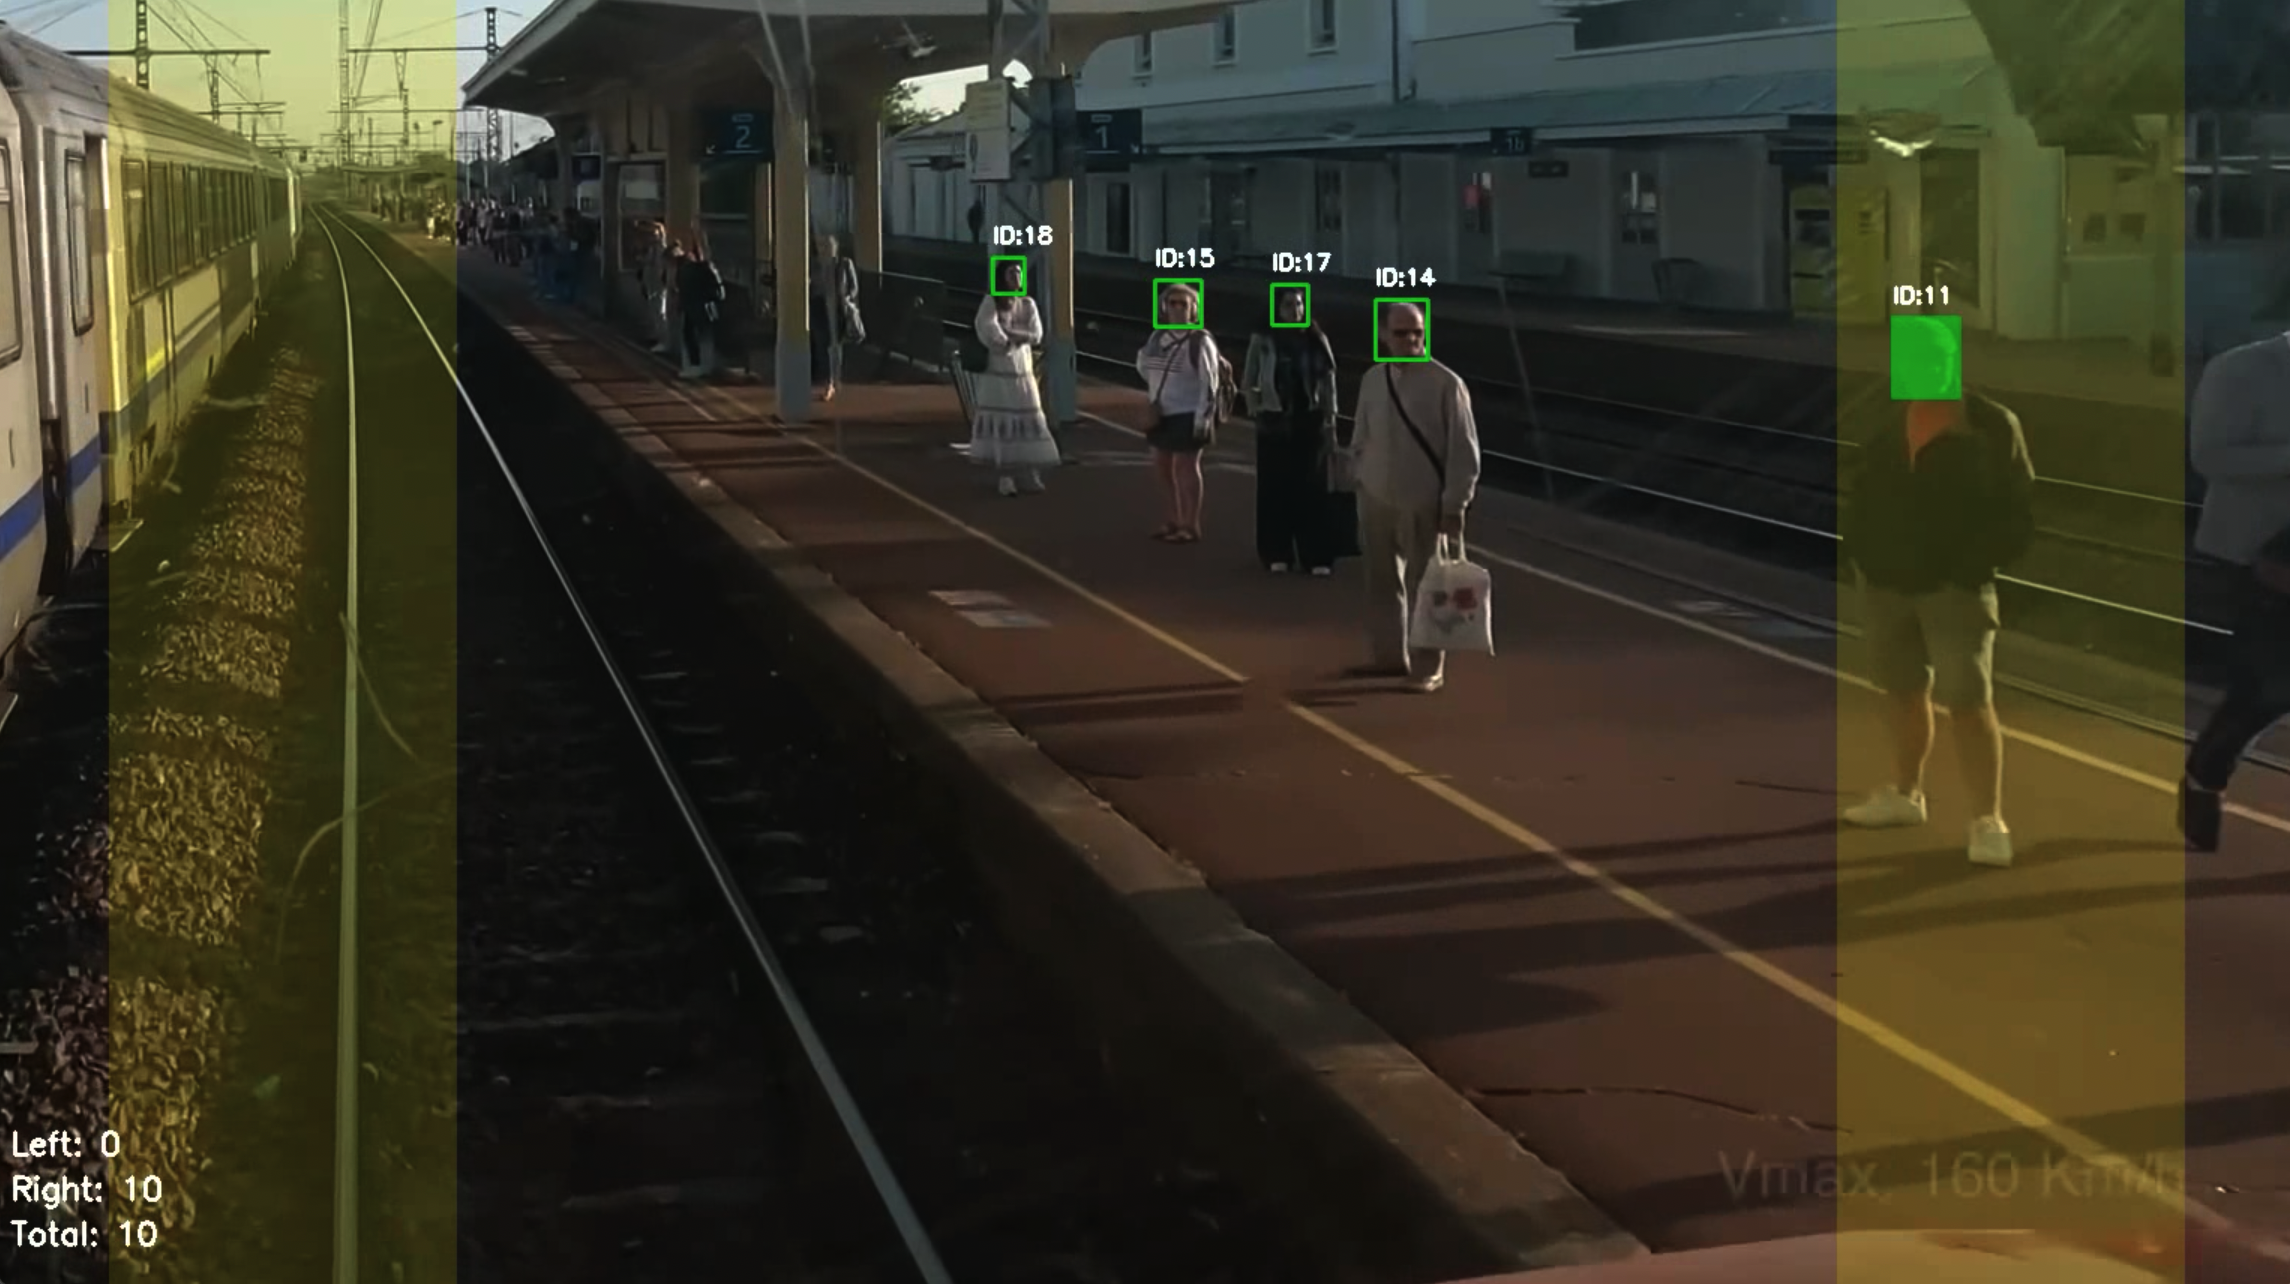
\includegraphics[width=0.8\textwidth]{pictures/CA12framedeomo.png}
    \caption{Intermediate tracking frame with the 12D state-vector model}
    \label{fig:CA12framedeomo}
\end{figure}

% --------------------------------------- Phys-5D ------------------------------------------------------------
\subsubsection{5D Physics-Constrained Model (Phys-5D)}
To overcome the limitations of image-plane kinematics, we introduce a 5D model that lifts estimation to 3D via pinhole geometry and scene priors.
\paragraph{5D Physically Constrained Model (Phys-5D).} We relate pixel height $h$ to depth $Z$ via $Z=fH/h$, with state \([u,v,h,Z,\dot{Z}]^\top\) and measurement \([u,v,h]^\top\). We explicitly update $Z$ and $h$ through projection and back-projection, and impose an adaptive deceleration prior on $\dot{Z}$ to reflect typical motion near the camera. Implementation references: \texttt{physical3dkf\_5d.py}, \texttt{deep\_sort/custom\_kf5d.py}.

\textbf{State:}
\begin{equation}
\mathbf{x}_k = [u, v, h_{px}, Z, \dot{Z}]^T \in \mathbb{R}^{5}
\end{equation}

\textbf{Geometric constraints:}
\begin{equation}
h_{px} = \frac{f \cdot H}{Z}, \quad Z = \frac{f \cdot H}{h_{px}}
\end{equation}
with focal length $f$ (pixels) and head height $H=0.3$ m.

\textbf{Depth dynamics:}
\begin{align}
Z_{k+1} &= Z_k + \dot{Z}_k \Delta t + \tfrac{1}{2}a_Z \Delta t^2 \\
\dot{Z}_{k+1} &= \dot{Z}_k + a_Z \Delta t
\end{align}

\textbf{Adaptive deceleration prior:}
\begin{equation}
a_Z = -\text{sign}(\dot{Z}) \cdot \min\Big(a_{max}, \frac{\dot{Z}^2}{2Z}\Big), \quad a_{max} = 1.0\,\text{m/s}^2
\end{equation}

\textbf{Process noise covariance:}
\begin{equation}
\mathbf{Q}_k = \text{diag}(\sigma_{pos}^2 h_{px}, \sigma_{pos}^2 h_{px}, \sigma_{pos}^2 h_{px}, \sigma_{vel}^2 h_{px}, \sigma_{vel}^2 h_{px})
\end{equation}
with $\sigma_{pos} = 1/2$, $\sigma_{vel} = 1/15$.

\textbf{Observation:}
\begin{equation}
\mathbf{z}_k = [u, v, h_{px}]^T \in \mathbb{R}^{3}
\end{equation}

\textbf{Observation matrix:}
\begin{equation}
\mathbf{H} = \begin{bmatrix}
1 & 0 & 0 & 0 & 0 \\
0 & 1 & 0 & 0 & 0 \\
0 & 0 & 1 & 0 & 0
\end{bmatrix}_{3 \times 5}
\end{equation}
We note that despite physics constraints, the model remains image-based and is influenced by image quality and calibration uncertainties. We use fSpy to estimate intrinsics on a representative frame: 2K right: $f=795.0$, $(c_x,c_y)=(268.0,137.0)$; 2K left: $f=795.0$, $(1268.0,137.0)$; 4K right: $f=1600.3$, $(515.0,153.0)$; 4K left: $f=1600.3$, $(1789.0,153.0)$.

On MOT-TPCH (20 videos), Phys-5D achieves average MOTA=67.21\%, MOTP=17.41\%, IDF1=76.29\%, IDP=82.23\%, IDR=71.51\%, ID Switches=24.8, FP=290, Precision=89.06\%, Recall=77.45\%, and counting MAPE=2.24\% (Table~\ref{tab:Phys5DResults}). Notably, identity switches regress to baseline levels (24.8 vs 24), far below CA-12D (39), while counting error reaches the best level. This demonstrates that physics priors regularize state evolution, avoiding identity confusion from 2D size fluctuations, and translating into superior counting.
\begin{table}[H]
\centering
\resizebox{\textwidth}{!}{%
\scriptsize
\renewcommand{\arraystretch}{1.5}
\begin{tabular}{p{0.5cm}|p{0.7cm}|p{0.7cm}|p{0.7cm}|p{0.7cm}|p{0.7cm}|p{0.8cm}|p{0.8cm}|p{0.8cm}|p{0.7cm}|p{0.6cm}|p{0.8cm}|p{0.7cm}|p{0.8cm}|p{0.8cm}|p{0.7cm}|p{0.8cm}|p{0.8cm}|p{0.8cm}|p{0.8cm}|p{0.8cm}}
\hline
{\tiny \textbf{Video}} & {\tiny \textbf{MOTA}} & {\tiny \textbf{MOTP}} & {\tiny \textbf{IDF1}} & {\tiny \textbf{IDP}} & {\tiny \textbf{IDR}} & {\tiny \textbf{IDS}} & {\tiny \textbf{Match-es}} & {\tiny \textbf{FP}} & {\tiny \textbf{Miss-es}} & {\tiny \textbf{FAF}} & {\tiny \textbf{Preci-sion}} & {\tiny \textbf{Recall}} & {\tiny \textbf{Mostly Track-ed}} & {\tiny \textbf{Partial-ly Track-ed}} & {\tiny \textbf{Mostly Lost}} & {\tiny \textbf{Left Count}} & {\tiny \textbf{Right Count}} & {\tiny \textbf{Total Count}} & {\tiny \textbf{Actual Count}} & {\tiny \textbf{MAPE}} \\ \hline
1 & 54.26 & 19.63 & 72.96 & 81.73 & 65.89 & 2 & 86 & 16 & 41 & 0.16 & 84.62 & 68.22 & 1 & 3 & 0 & 0 & 4 & 4 & 4 & 0 \\
\rowcolor{gray!10}
2 & 57.35 & 17.64 & 75.65 & 87.65 & 66.55 & 3 & 375 & 51 & 187 & 0.22 & 88.11 & 66.9 & 3 & 5 & 0 & 8 & 0 & 8 & 8 & 0 \\
3 & 57.25 & 17.66 & 73.19 & 77.53 & 69.32 & 7 & 993 & 215 & 359 & 0.52 & 82.3 & 73.58 & 12 & 10 & 3 & 24 & 0 & 25 & 25 & 0 \\
\rowcolor{gray!10}
4 & 78.33 & 16.74 & 83.16 & 81.49 & 84.9 & 1 & 610 & 86 & 58 & 0.29 & 87.66 & 91.33 & 9 & 1 & 0 & 0 & 10 & 10 & 10 & 0 \\
5 & 64.42 & 16.5 & 78.33 & 79.56 & 77.14 & 3 & 874 & 175 & 208 & 0.36 & 83.37 & 80.83 & 13 & 4 & 1 & 19 & 0 & 19 & 18 & 5.56 \\
\rowcolor{gray!10}
6 & 81.1 & 16.11 & 82.98 & 84.91 & 81.13 & 8 & 2440 & 196 & 319 & 0.29 & 92.59 & 88.47 & 13 & 3 & 0 & 16 & 0 & 16 & 16 & 0 \\
7 & 53.72 & 19.9 & 63.01 & 75.52 & 54.06 & 15 & 1097 & 150 & 651 & 0.29 & 88.11 & 63.07 & 6 & 10 & 5 & 0 & 21 & 21 & 21 & 0 \\
\rowcolor{gray!10}
8 & 57.31 & 16.91 & 74.24 & 81.18 & 68.39 & 17 & 2522 & 473 & 1036 & 0.44 & 84.3 & 71.02 & 20 & 23 & 4 & 1 & 44 & 44 & 47 & 6.38 \\
9 & 73.84 & 15.94 & 79.76 & 88.47 & 72.6 & 87 & 10968 & 537 & 3071 & 0.26 & 95.37 & 78.26 & 71 & 51 & 2 & 0 & 123 & 123 & 124 & 0.81 \\
\rowcolor{gray!10}
10 & 78.67 & 18.02 & 85.86 & 88.98 & 82.96 & 12 & 1517 & 123 & 243 & 0.19 & 92.55 & 86.29 & 14 & 5 & 0 & 19 & 0 & 19 & 19 & 0 \\
11 & 71.41 & 19.41 & 76.45 & 80.95 & 72.43 & 35 & 2507 & 266 & 596 & 0.33 & 90.53 & 81.01 & 18 & 8 & 1 & 27 & 0 & 27 & 27 & 0 \\
\rowcolor{gray!10}
12 & 68.76 & 19.79 & 72.11 & 79.28 & 66.13 & 94 & 8403 & 766 & 2609 & 0.33 & 91.73 & 76.51 & 36 & 27 & 1 & 66 & 0 & 66 & 64 & 3.12 \\
13 & 76.76 & 15.26 & 83.84 & 92.13 & 76.92 & 4 & 498 & 19 & 122 & 0.08 & 96.35 & 80.45 & 8 & 4 & 0 & 11 & 0 & 12 & 12 & 0 \\
\rowcolor{gray!10}
14 & 56.74 & 17.15 & 66.1 & 74.66 & 59.31 & 119 & 8217 & 1320 & 3819 & 0.7 & 86.33 & 68.58 & 34 & 58 & 7 & 0 & 100 & 100 & 100 & 0 \\
15 & 62.28 & 17.2 & 71.93 & 78.18 & 66.62 & 16 & 1947 & 296 & 688 & 0.43 & 86.9 & 74.05 & 16 & 10 & 2 & 29 & 0 & 29 & 28 & 3.57 \\
\rowcolor{gray!10}
16 & 63.13 & 17.31 & 74.31 & 75.3 & 73.35 & 17 & 2850 & 602 & 694 & 0.48 & 82.65 & 80.51 & 21 & 11 & 0 & 0 & 31 & 32 & 32 & 0 \\
17 & 72.73 & 15.43 & 82.94 & 84.76 & 81.2 & 11 & 1218 & 162 & 223 & 0.34 & 88.35 & 84.64 & 11 & 4 & 1 & 0 & 15 & 15 & 16 & 6.25 \\
\rowcolor{gray!10}
18 & 79.97 & 15.45 & 70.53 & 73.22 & 68.03 & 6 & 1119 & 81 & 173 & 0.12 & 93.28 & 86.67 & 3 & 3 & 0 & 6 & 0 & 6 & 6 & 0 \\
19 & 75.37 & 17.63 & 84.94 & 89.28 & 81 & 5 & 1073 & 97 & 217 & 0.34 & 91.74 & 83.24 & 15 & 7 & 2 & 0 & 21 & 21 & 24 & 12.5 \\
\rowcolor{gray!10}
20 & 60.73 & 18.45 & 73.56 & 89.79 & 62.29 & 34 & 2859 & 174 & 1528 & 0.18 & 94.33 & 65.44 & 12 & 32 & 2 & 43 & 0 & 43 & 46 & 6.52 \\
\rowcolor{gray!20}
Avg. & 67.21 & 17.41 & 76.29 & 82.23 & 71.51 & 24.80 & 2609 & 290 & 842 & 0.32 & 89.06 & 77.45 & 16.80 & 13.95 & 1.55 & 13.45 & 18.45 & 32.00 & 32.35 & 2.24 \\ \hline
\end{tabular}%
}
\caption{Phys-5-Dimensional State Vector Model MOT and Count Evaluation Results}
\label{tab:Phys5DResults}
\end{table}

\begin{figure}[H]
    \centering
    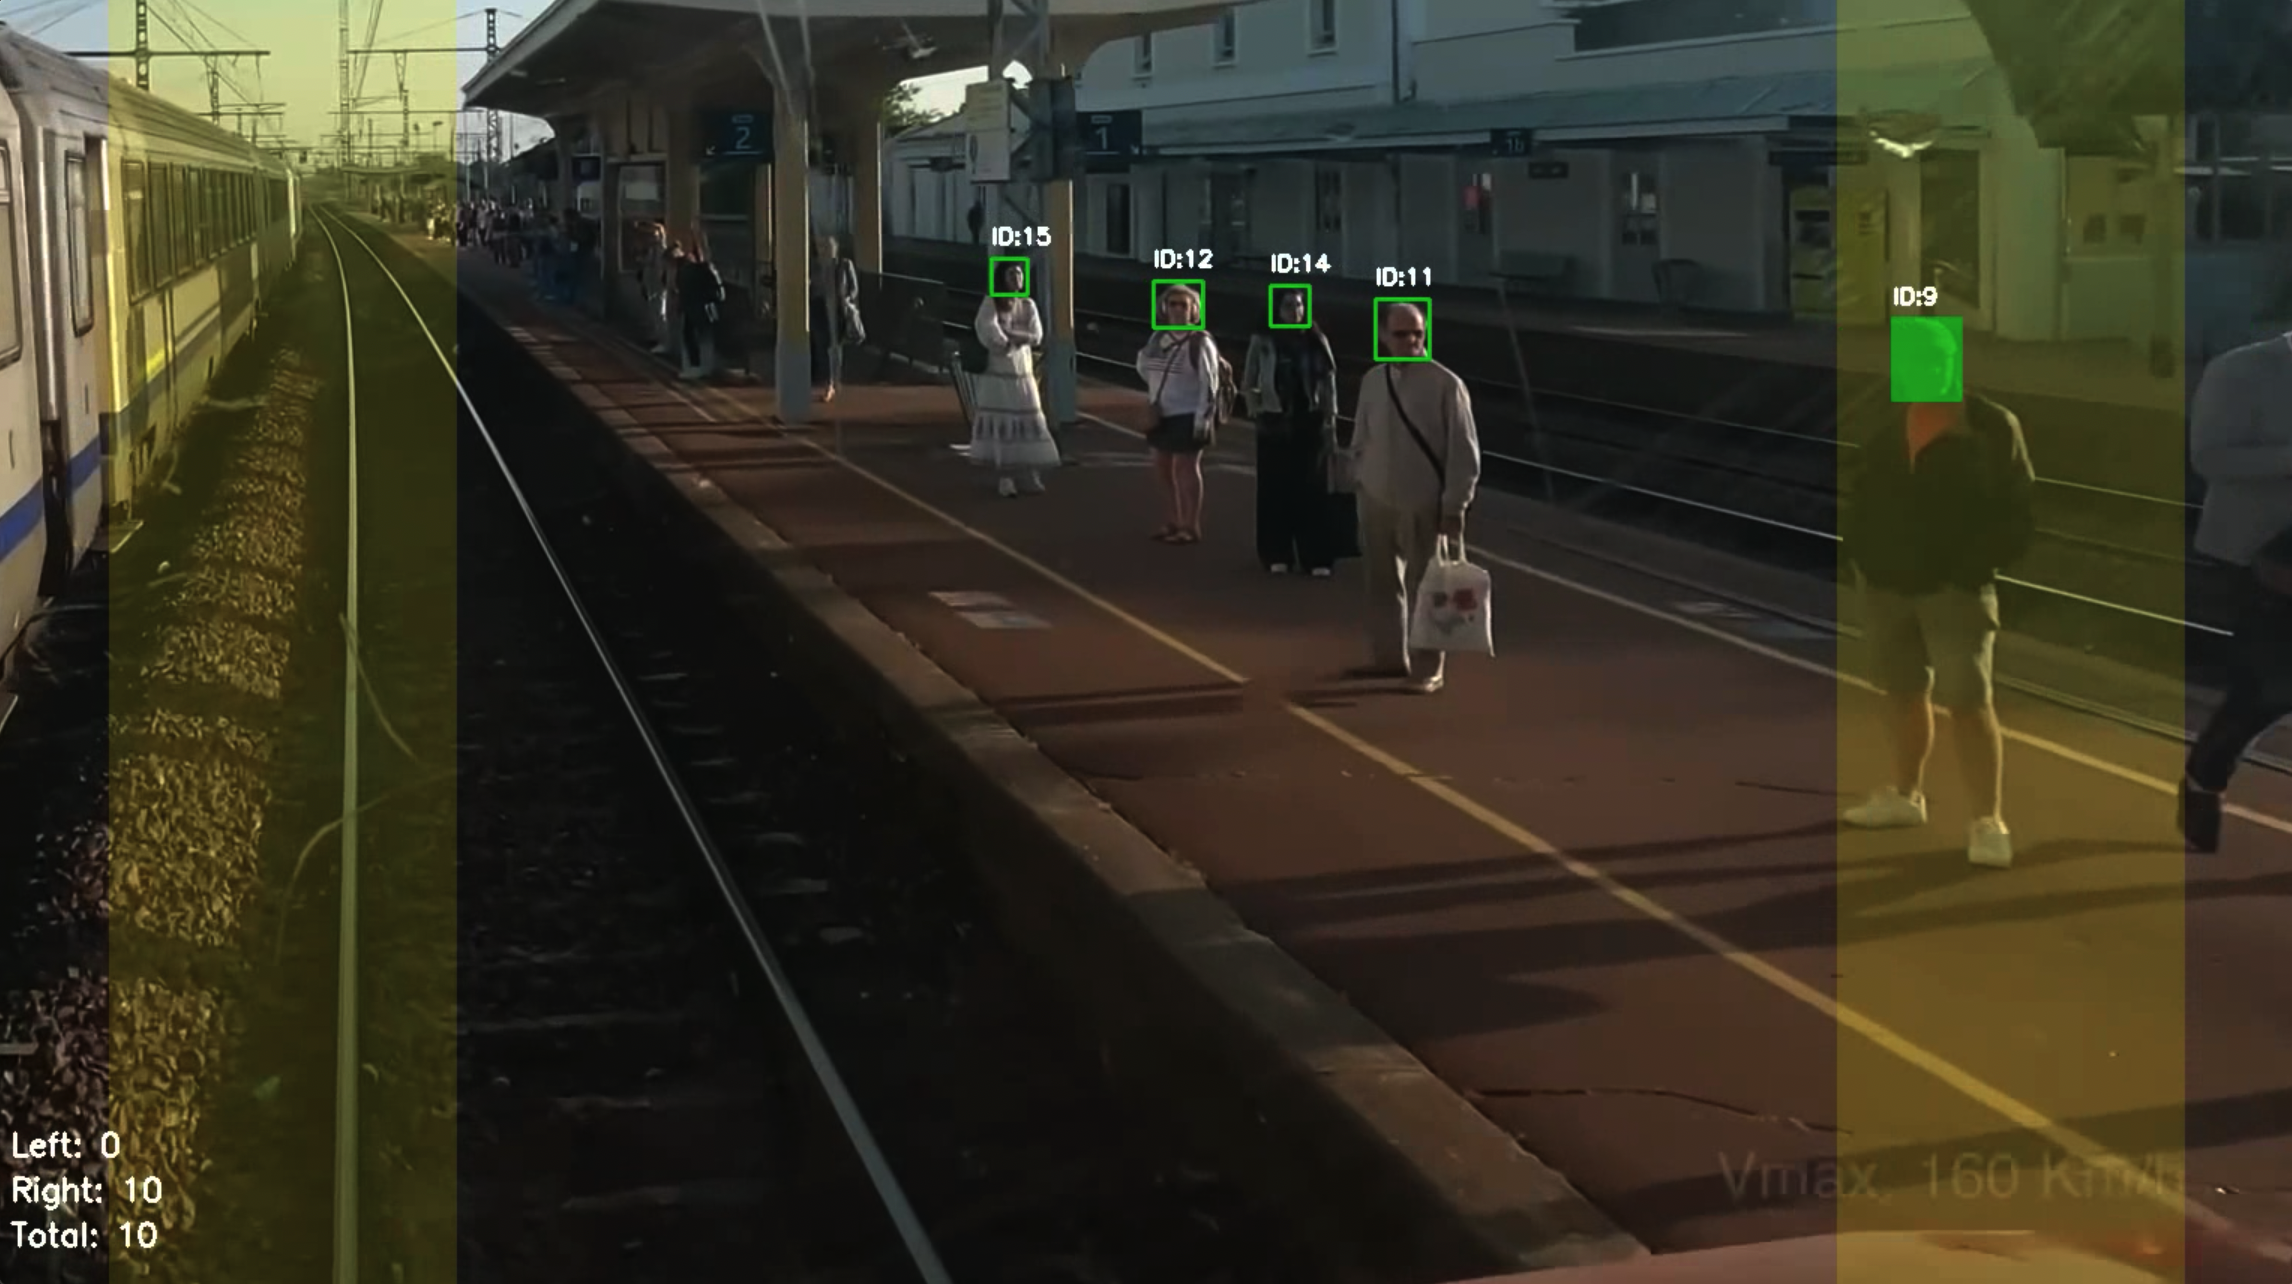
\includegraphics[width=0.8\textwidth]{pictures/Phys5Dframedeomo.png}
    \caption{Intermediate tracking frame with the 5D state-vector model}
    \label{fig:Phys5Dframedeomo}
\end{figure}
In summary, Phys-5D integrates camera geometry and motion priors to lift from 2D to 3D reasoning, greatly stabilizing trajectories and identity consistency, and achieving the best counting accuracy.


\subsubsection{Evaluation Across Three Motion Models}
Following the Chapter 4 metrics, Table~\ref{tab:3modelsCountingComparisonResults} compares counting performance. Phys-5D achieves the best MAE/RMSE/MAPE/ME.
\begin{table}[H]
    \centering
    \begin{tabular}{ccccc}
    \hline
        \textbf{Model} & \textbf{MAE } & \textbf{RMSE} & \textbf{MAPE(\%)} & \textbf{ME } \\ \hline
        \textbf{CV-8D} & 3.4 & 6.1514 & 14.592 & 1.4  \\
        \textbf{CA-12D} & 2.4 & 4.5837 & 6.99 & 0.7  \\
        \textbf{Phys-5D} & 0.75 & 1.3229 & 2.236 & -0.25 \\ \hline
    \end{tabular}
    \caption{Comparison of Counting Performance Across Three Motion Models}
    \label{tab:3modelsCountingComparisonResults}
\end{table}
Key observations: (1) Complexity does not monotonically improve performance—while CA-12D reduces counting error relative to CV-8D, it harms identity stability; (2) incorporating domain priors is crucial—Phys-5D (lower dimensional yet physically constrained) delivers the best identity consistency and counting accuracy.


\subsection{Ablation of the Counting Method}
We evaluate the proposed Virtual Counting Band and its hyperparameters. The band introduces nonzero width and a persistence criterion to overcome line-crossing brittleness under jitter and occlusion. We focus on the start and end positions.

As in Figure~\ref{fig:VirtualCountingZone}, start and end denote distances from the image borders relative to width (e.g., Start=0.05, End=0.20 defines a band from 0.05×W to 0.20×W on both sides). Start=End degenerates to a line.
\begin{figure}[H]
    \centering
    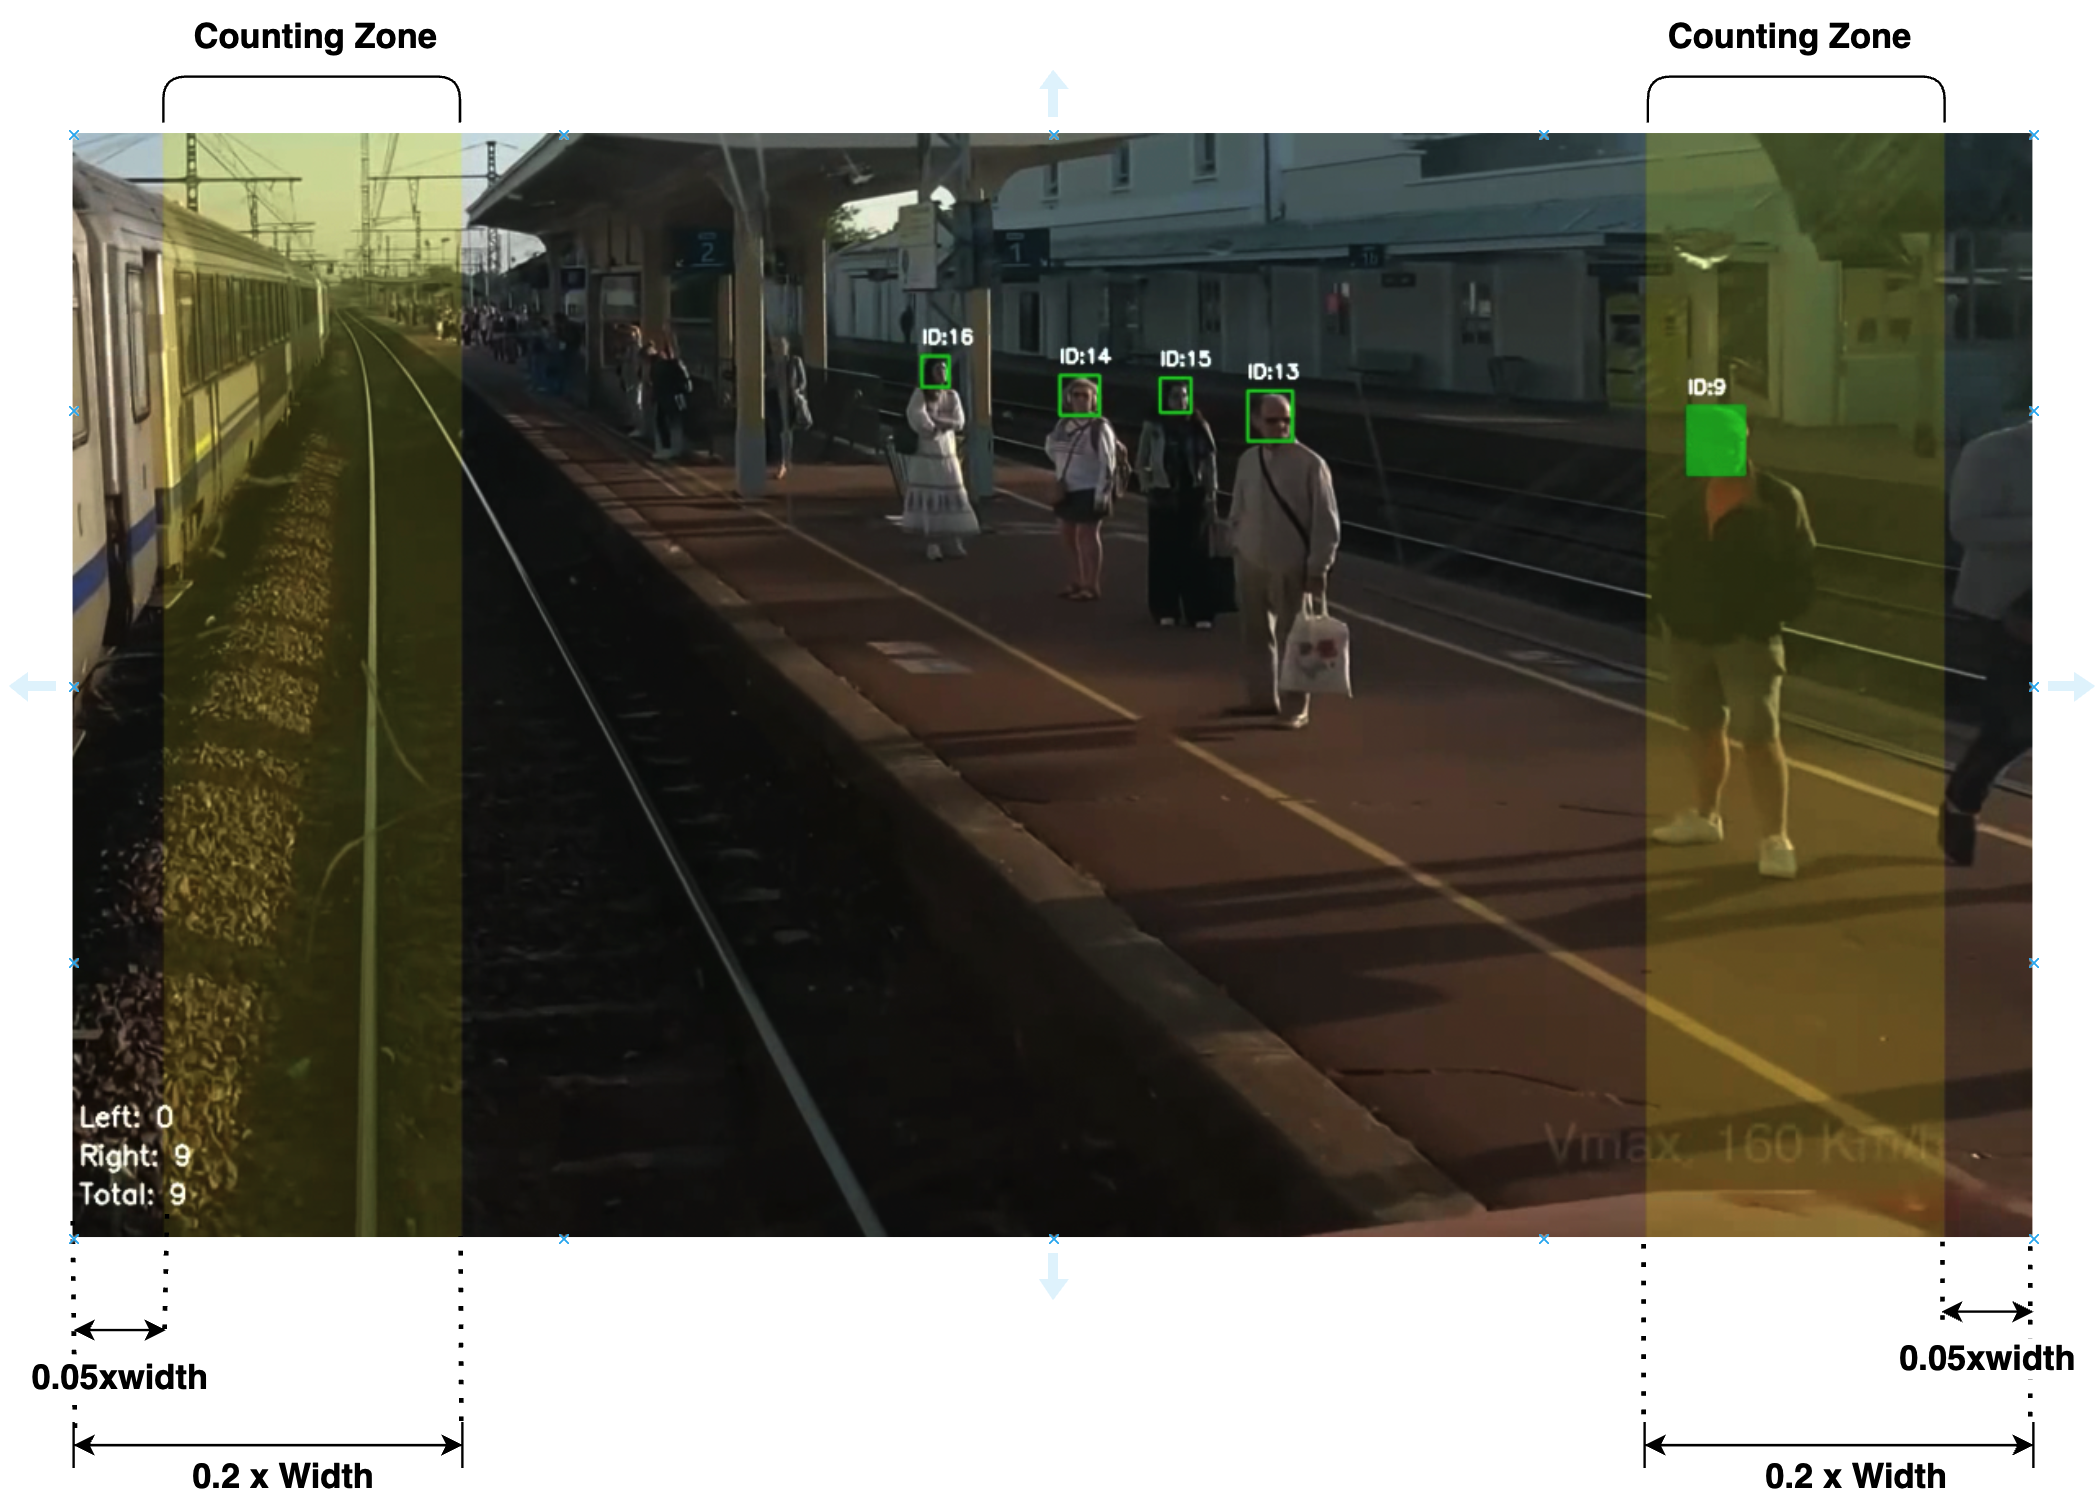
\includegraphics[width=0.8\textwidth]{pictures/VirtualCountingZone.png}
    \caption{Schematic Diagram of the Virtual Counting Zone}
    \label{fig:VirtualCountingZone}
\end{figure}

Table~\ref{tab:CountingbandAblationExperiment} reports results across configurations. Performance is highly sensitive to width and position, revealing an optimal range.
\begin{table}[H]
    \centering
    \resizebox{0.6\textwidth}{!}{%
    \begin{tabular}{cccccc}
    \hline
        \textbf{Start} & \textbf{End} & \textbf{MAE} & \textbf{RMSE} & \textbf{MAPE(\%)} & \textbf{ME } \\ \hline
        \rowcolor{gray!30}
        0.05  & 0.20  & 0.90  & 1.38  & 2.97  & -0.20   \\
        \rowcolor{gray!10}
        0.05  & 0.15  & 1.15  & 1.75  & 4.07  & -0.95   \\
        0.00  & 0.15  & 1.25  & 1.77  & 4.67  & -0.15   \\
        \rowcolor{gray!10}
        0.10  & 0.20  & 1.40  & 2.10  & 5.28  & -1.10   \\
        0.00  & 0.20  & 1.50  & 2.14  & 4.97  & 0.60   \\
        \rowcolor{gray!10}
        0.15  & 0.30  & 1.50  & 2.37  & 8.58  & 0.20   \\
        0.00  & 0.10  & 1.80  & 2.57  & 5.83  & -1.60   \\
        \rowcolor{gray!10}
        0.10  & 0.25  & 1.80  & 2.68  & 6.94  & 0.30   \\
        0.20  & 0.30  & 2.05  & 2.89  & 9.66  & -0.85   \\
        \rowcolor{gray!10}
        0.05  & 0.25  & 2.10  & 2.93  & 6.55  & 1.10   \\
        0.15  & 0.25  & 2.10  & 2.81  & 9.57  & -1.30   \\
        \rowcolor{gray!10}
        0.20  & 0.35  & 2.40  & 3.44  & 10.61  & 1.10   \\
        0.10  & 0.30  & 2.45  & 3.68  & 8.55  & 1.65   \\
        \rowcolor{gray!10}
        0.10  & 0.15  & 2.60  & 3.65  & 9.81  & -2.50   \\
        0.00  & 0.25  & 2.75  & 3.94  & 8.59  & 1.85   \\
        \rowcolor{gray!10}
        0.05  & 0.10  & 2.75  & 3.56  & 8.78  & -2.55   \\
        0.05  & 0.30  & 2.85  & 4.46  & 8.56  & 2.45   \\
        \rowcolor{gray!10}
        0.15  & 0.35  & 2.85  & 4.42  & 11.16  & 1.95   \\
        0.30  & 0.40  & 3.05  & 4.17  & 15.38  & -0.55   \\
        \rowcolor{gray!10}
        0.15  & 0.20  & 3.15  & 4.38  & 11.45  & -3.05   \\
        0.20  & 0.25  & 3.50  & 4.93  & 12.89  & -2.80   \\
        \rowcolor{gray!10}
        0.30  & 0.35  & 3.50  & 4.43  & 16.85  & -3.40   \\
        0.00  & 0.30  & 3.60  & 5.53  & 10.81  & 3.20   \\
        \rowcolor{gray!10}
        0.10  & 0.35  & 3.90  & 6.43  & 11.85  & 3.30   \\
        0.20  & 0.40  & 4.15  & 6.43  & 16.10  & 3.35   \\
        \rowcolor{gray!10}
        0.05  & 0.35  & 4.30  & 7.44  & 11.85  & 4.10   \\
        0.15  & 0.40  & 4.65  & 7.55  & 16.81  & 4.15   \\
        \rowcolor{gray!10}
        0.00  & 0.35  & 5.00  & 8.54  & 13.79  & 4.80   \\
        0.10  & 0.40  & 5.80  & 9.62  & 17.90  & 5.50   \\
        \rowcolor{gray!10}
        0.00  & 0.05  & 5.95  & 7.77  & 18.77  & -5.95   \\
        0.05  & 0.40  & 6.30  & 10.62  & 18.11  & 6.30   \\
        \rowcolor{gray!10}
        0.00  & 0.40  & 7.00  & 11.72  & 20.05  & 7.00   \\
        0.30  & 0.30  & 31.10  & 43.49  & 92.71  & -31.10   \\
        \rowcolor{gray!10}
        0.05  & 0.05  & 31.30  & 43.69  & 93.55  & -31.30   \\
        0.15  & 0.15  & 31.30  & 43.67  & 93.58  & -31.30   \\
        \rowcolor{gray!10}
        0.10  & 0.10  & 31.35  & 43.74  & 93.66  & -31.35   \\ \hline
    \end{tabular}%
    }
    \label{tab:CountingbandAblationExperiment}
    \caption{Results of Counting Zone and Line Ablation Experiment}
\end{table}
Best configuration: Start=0.05, End=0.20 achieves MAE=0.90, RMSE=1.38, MAPE=2.97\%, ME=−0.20, indicating near-unbiased counting with minimal variance. In contrast, degenerate line settings (Start=End) cause catastrophic degradation (e.g., MAE≈31.3, MAPE>93\%, ME≈−31.3), evidencing severe undercounting due to sensitivity to jitter and transient detection loss. Excessively wide bands inflate overcounting risk through longer dwell times and potential ID switches (e.g., Start=0.00, End=0.40 with MAE=7.00, RMSE=11.72, ME=+7.00).

Table~\ref{tab:ComparisonofAverage} further contrasts average metrics for line vs band: the band dramatically outperforms the line across MAE, RMSE, MAPE, and ME, demonstrating superior robustness and accuracy.
\begin{table}[H]
    \centering
    \begin{tabular}{ccccc}
    \hline
        \textbf{} & \textbf{MAE} & \textbf{RMSE} & \textbf{MAPE(\%)} & \textbf{ME } \\ \hline
        Average metrics of line-crossing counting & 31.28  & 43.66  & 93.43  & -31.28   \\
        Average counting metrics of counting zones & 3.13  & 4.75  & 10.87  & 0.81  \\ \hline
    \end{tabular}
    \caption{Comparison of Average Counting Metrics Lines vs. Zones}
    \label{tab:ComparisonofAverage}
\end{table}

\subsection{Summary}
We validate the detect–track–count framework comprehensively:
\begin{itemize}
    \item High-accuracy detector: two-stage training yields mAP50 from 79.4\%→98.0\% and mAP50–95 from 54.7\%→81.6\% on target data.
    \item Tracking model comparison: CA-12D lowers counting MAPE to 6.99\% but increases ID switches; Phys-5D achieves the best overall trade-off with MAPE=2.24\% and MAE=0.75 while maintaining identity consistency comparable to CV-8D.
    \item Counting method ablation: the proposed virtual band (Start=0.05, End=0.20) far outperforms line-crossing (e.g., MAE=0.90 vs 31.28; MAPE=2.97\% vs 93.43\%), confirming the necessity of width and persistence.
\end{itemize}
Overall, the combination of YOLOv11m (detector) + Phys-5D (tracker) + optimized virtual counting band constitutes an effective solution for platform crowd counting, delivering robust identity preservation and state-of-the-art counting accuracy.

\iffalse

% -------------------------以下是中文版本---------------------------------------%
本章围绕"检测—跟踪—计数"的整体流程，系统评估了所提出的人群头部检测与站台场景多目标跟踪计数方法。我们以YOLO11m作为检测器，结合基于EfficientNet-B0 的ReID外观描述模型，并在DeepSORT框架内分别接入三类运动模型以开展实验，包括：8维度匀速基准模型（标准DeepSORT卡尔曼滤波器）；12维度加速度模型以及结合针孔相机集合约束的5维度物理模型。在Data章节所提供的具有MOT标注格式的数据上进行评估，其中检测器训练与微调所用的静态图像数据集与多段视频序列互相补充，既涵盖了通用的拥挤场景，也覆盖了列车进站期间不同密度的平台场景。


1.检测器YOLO11m的训练与微调
如 \S\ref{section::Methods} 所述，我们选用YOLO11m作为精度与速度的折中版本。本节对检测器 YOLOv11m 的训练与微调过程进行详细评估。我们采用了一种两阶段迁移学习（Two-Stage Transfer Learning）*的策略，旨在构建一个既具备泛化能力又在目标场景下性能卓越的头部检测器，为后续的多目标跟踪任务奠定坚实的基础。训练过程分为两个阶段：第一阶段在CrowdHuman数据集上进行预训练，以获得通用头部检测能力；第二阶段采用冻结主干网络（backbone=10）的微调策略，使用我们整合标注的Open Sensor Data for Rail 2023、RailEye3D以及自建TrainPlatformCrowd三个数据集中的共2,000张头部标注图像进行训练，最终得到检测器权重文件YOLO11freeze10.pt。

训练超参数设置如下：两个阶段均训练100个epoch，使用SGD优化器，初始学习率为0.01，动量0.937，权重衰减0.0005。其余参数遵循YOLO系列模型的默认设置。

预训练阶段的核心目标是让模型从大规模、多样化的数据集中学习人类头部的通用、鲁棒的视觉特征。为此，我们选用了业界公认的 CrowdHuman 数据集。如第三章Data \S\ref{section::data}所示，该数据集大量的实例，为深度神经网络提供了丰富的学习样本。
第一阶段在CrowdHuman数据集上的训练结果如\ref{fig:yolo11mpre2results}"和表\ref{tab:yolopre2_results}所示，模型在该数据集上达到了79.4\%的mAP50 和 54.7\%的mAP50–95.
\begin{figure}[H]
    \centering
    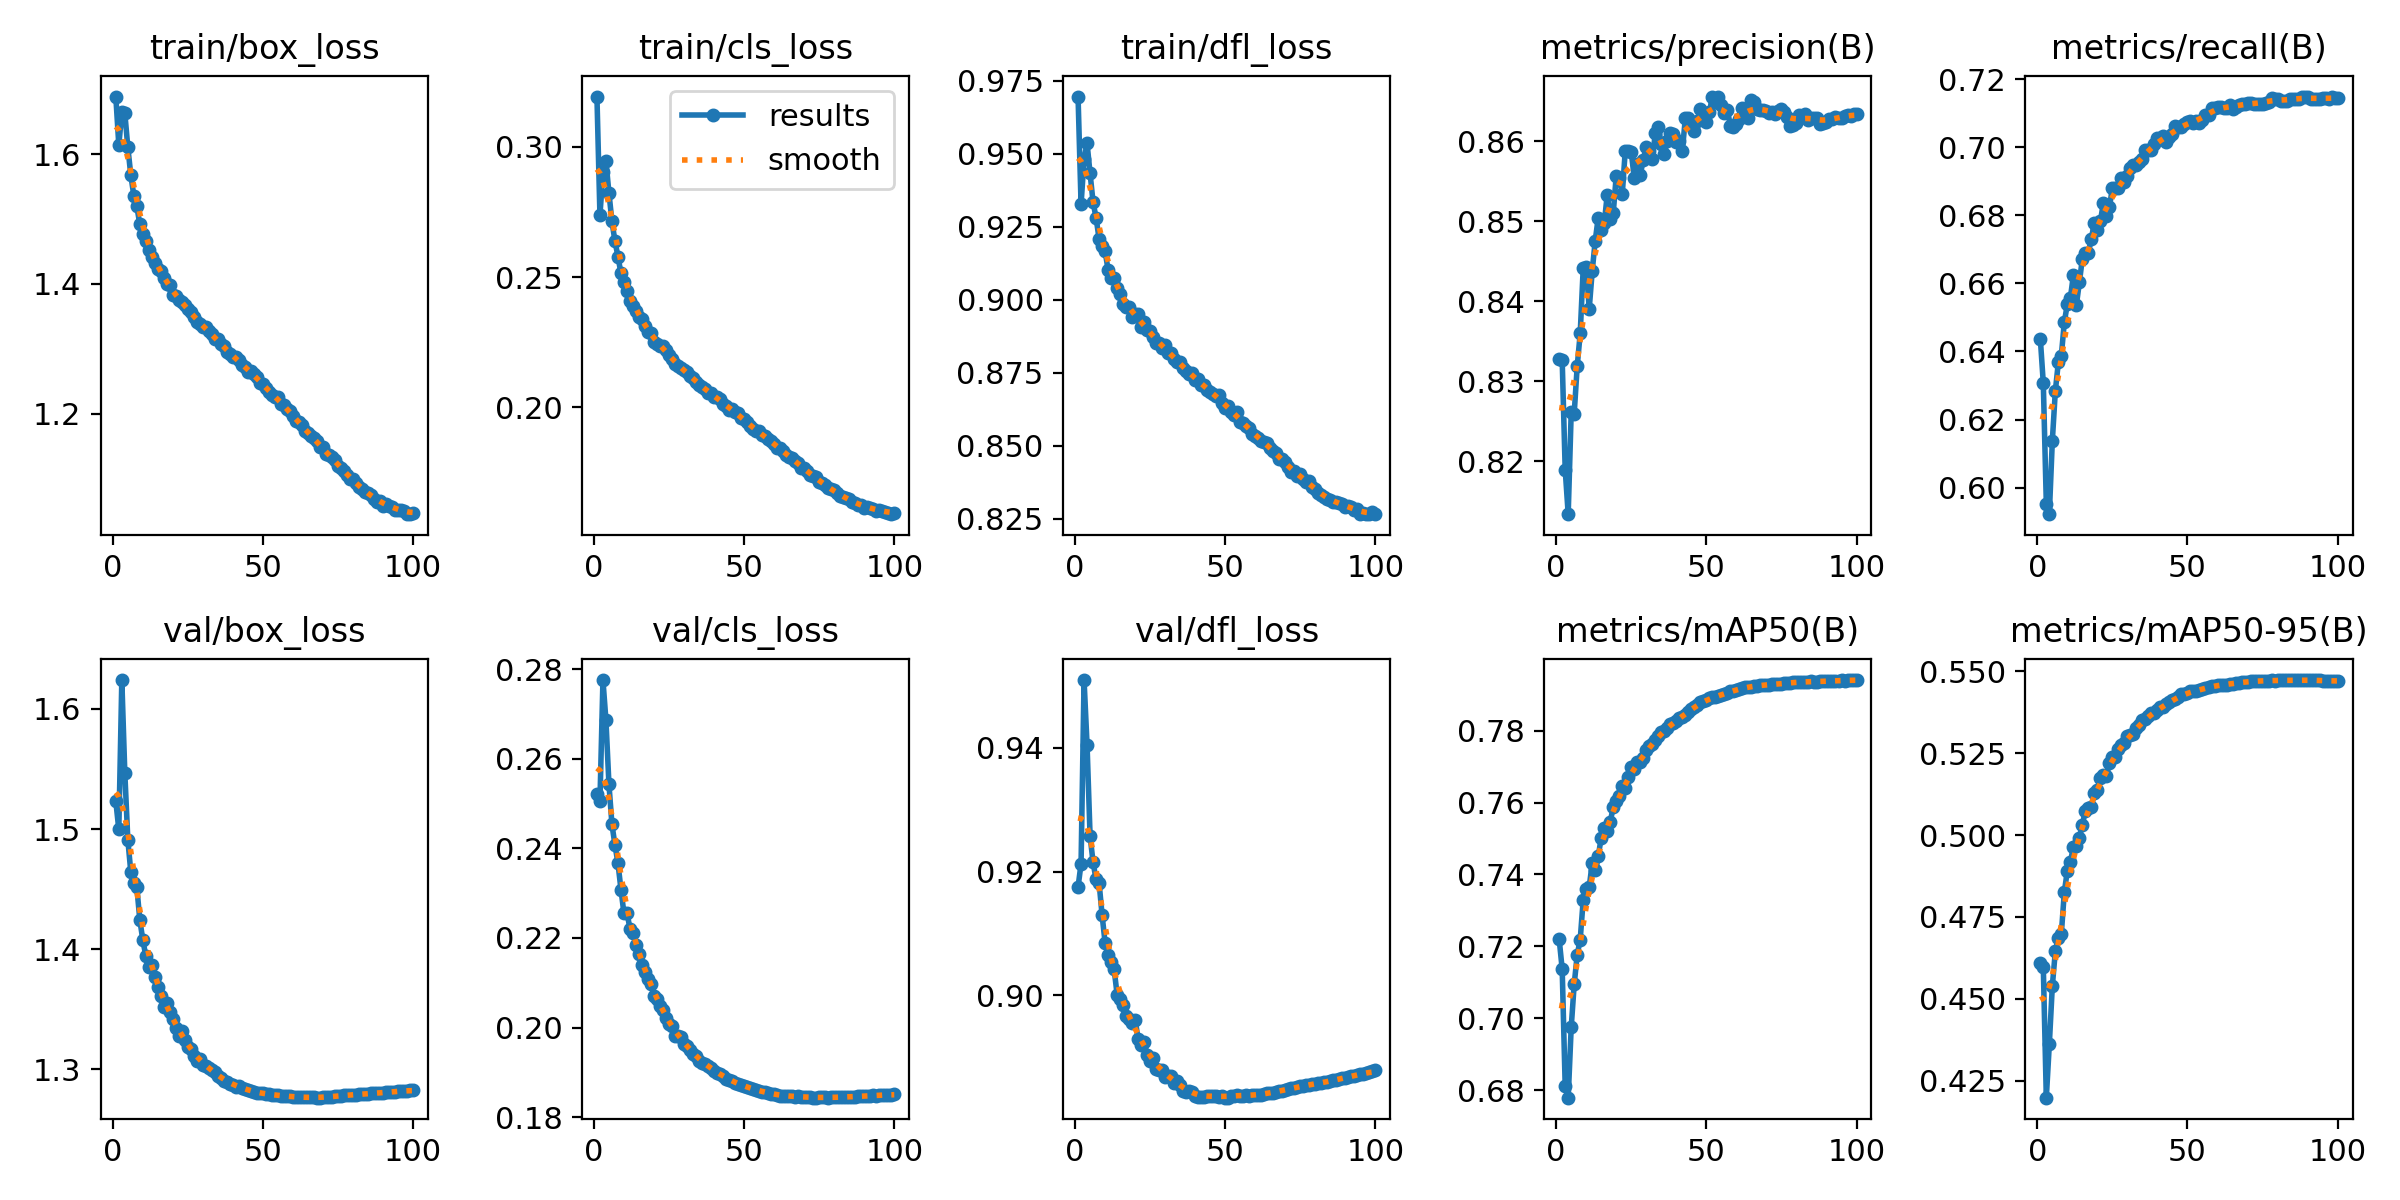
\includegraphics[width=0.8\textwidth]{pictures/yolo11mpre2results.png}
    \caption{Pre-training Results of YOLOv11m on the CrowdHuman Dataset}
    \label{fig:yolo11mpre2results}
\end{figure}

\begin{table}[H]
\centering
\setlength{\tabcolsep}{12pt}
\renewcommand{\arraystretch}{1.3}
\begin{tabular}{|c|c|c|c|c|c|c|}
\hline
\textbf{Class} & \textbf{Images} & \textbf{Instances} & \textbf{Box(Precision)} & \textbf{Recall} & \textbf{mAP50} & \textbf{mAP50–95} \
\hline
\rowcolor{blue!20}
all & 4370 & 98568 & 0.862 & 0.715 & 0.794 & 0.547 \
\hline
\end{tabular}
\caption{Pre-training Performance of YOLOv11m on the CrowdHuman Dataset}
\label{tab:yolopre2_results}
\end{table}
这一性能指标表明，模型已成功建立起对人类头部的基本检测能力。其中，mAP50 反映了模型在较为宽松的交并比（IoU）阈值下的检测准确率，而 mAP50-95 则代表了在更严格、连续的IoU阈值下的平均精度，后者更能衡量检测框的定位精确度。此阶段的结果证明，模型已经构建了一个坚实的特征提取基础，但其定位精度在复杂场景下仍有提升空间。


第二阶段，我们进入了微调阶段。此阶段的核心思想是领域自适应（Domain Adaptation）。我们采用了由 Open Sensor Data for Rail 2023、RailEye3D 及自建数据集共同组成的、高度针对性的头部标注图像。
微调策略上，我们冻结了主干网络（backbone）的前10层。这一决策基于以下考量：网络模型的浅层部分通常学习到的是边缘、颜色、纹理等通用性强的低级特征，这些特征在不同数据集间是高度可迁移的。通过冻结这些层，我们保留了在CrowdHuman数据集上学到的宝贵通用知识，防止其在小规模数据集上微调时被"遗忘"；同时，我们仅训练网络的深层部分，使其专注于学习站台场景特有的高级语义特征（如光照、遮挡模式、人群分布等），从而实现了高效且精准的知识迁移。

微调结果如\ref{fig:yolo11mfinetuneresults}和表\ref{tab:yolofreeze10_results}所示，微调后的模型性能获得了质的飞跃。mAP50 从79.4\% 提升至 98.0\%（提升了18.6个百分点），而mAP50-95 从54.7\% 显著提升至 81.6\%（提升了26.9个百分点）。这一结果有力地证明了我们两阶段训练策略的有效性。尤其值得关注的是 mAP50-95 的大幅增长，这表明模型不仅能准确识别出头部目标，其定位精度（Localization Accuracy）也得到了根本性的改善。对于"检测—跟踪—计数"这一环环相扣的流程而言，一个高精度的检测器是后续任务成功的关键前提，因为精确的边界框（bounding box）能够显著降低跟踪过程中的ID切换和轨迹漂移风险。

\begin{figure}[H]
    \centering
    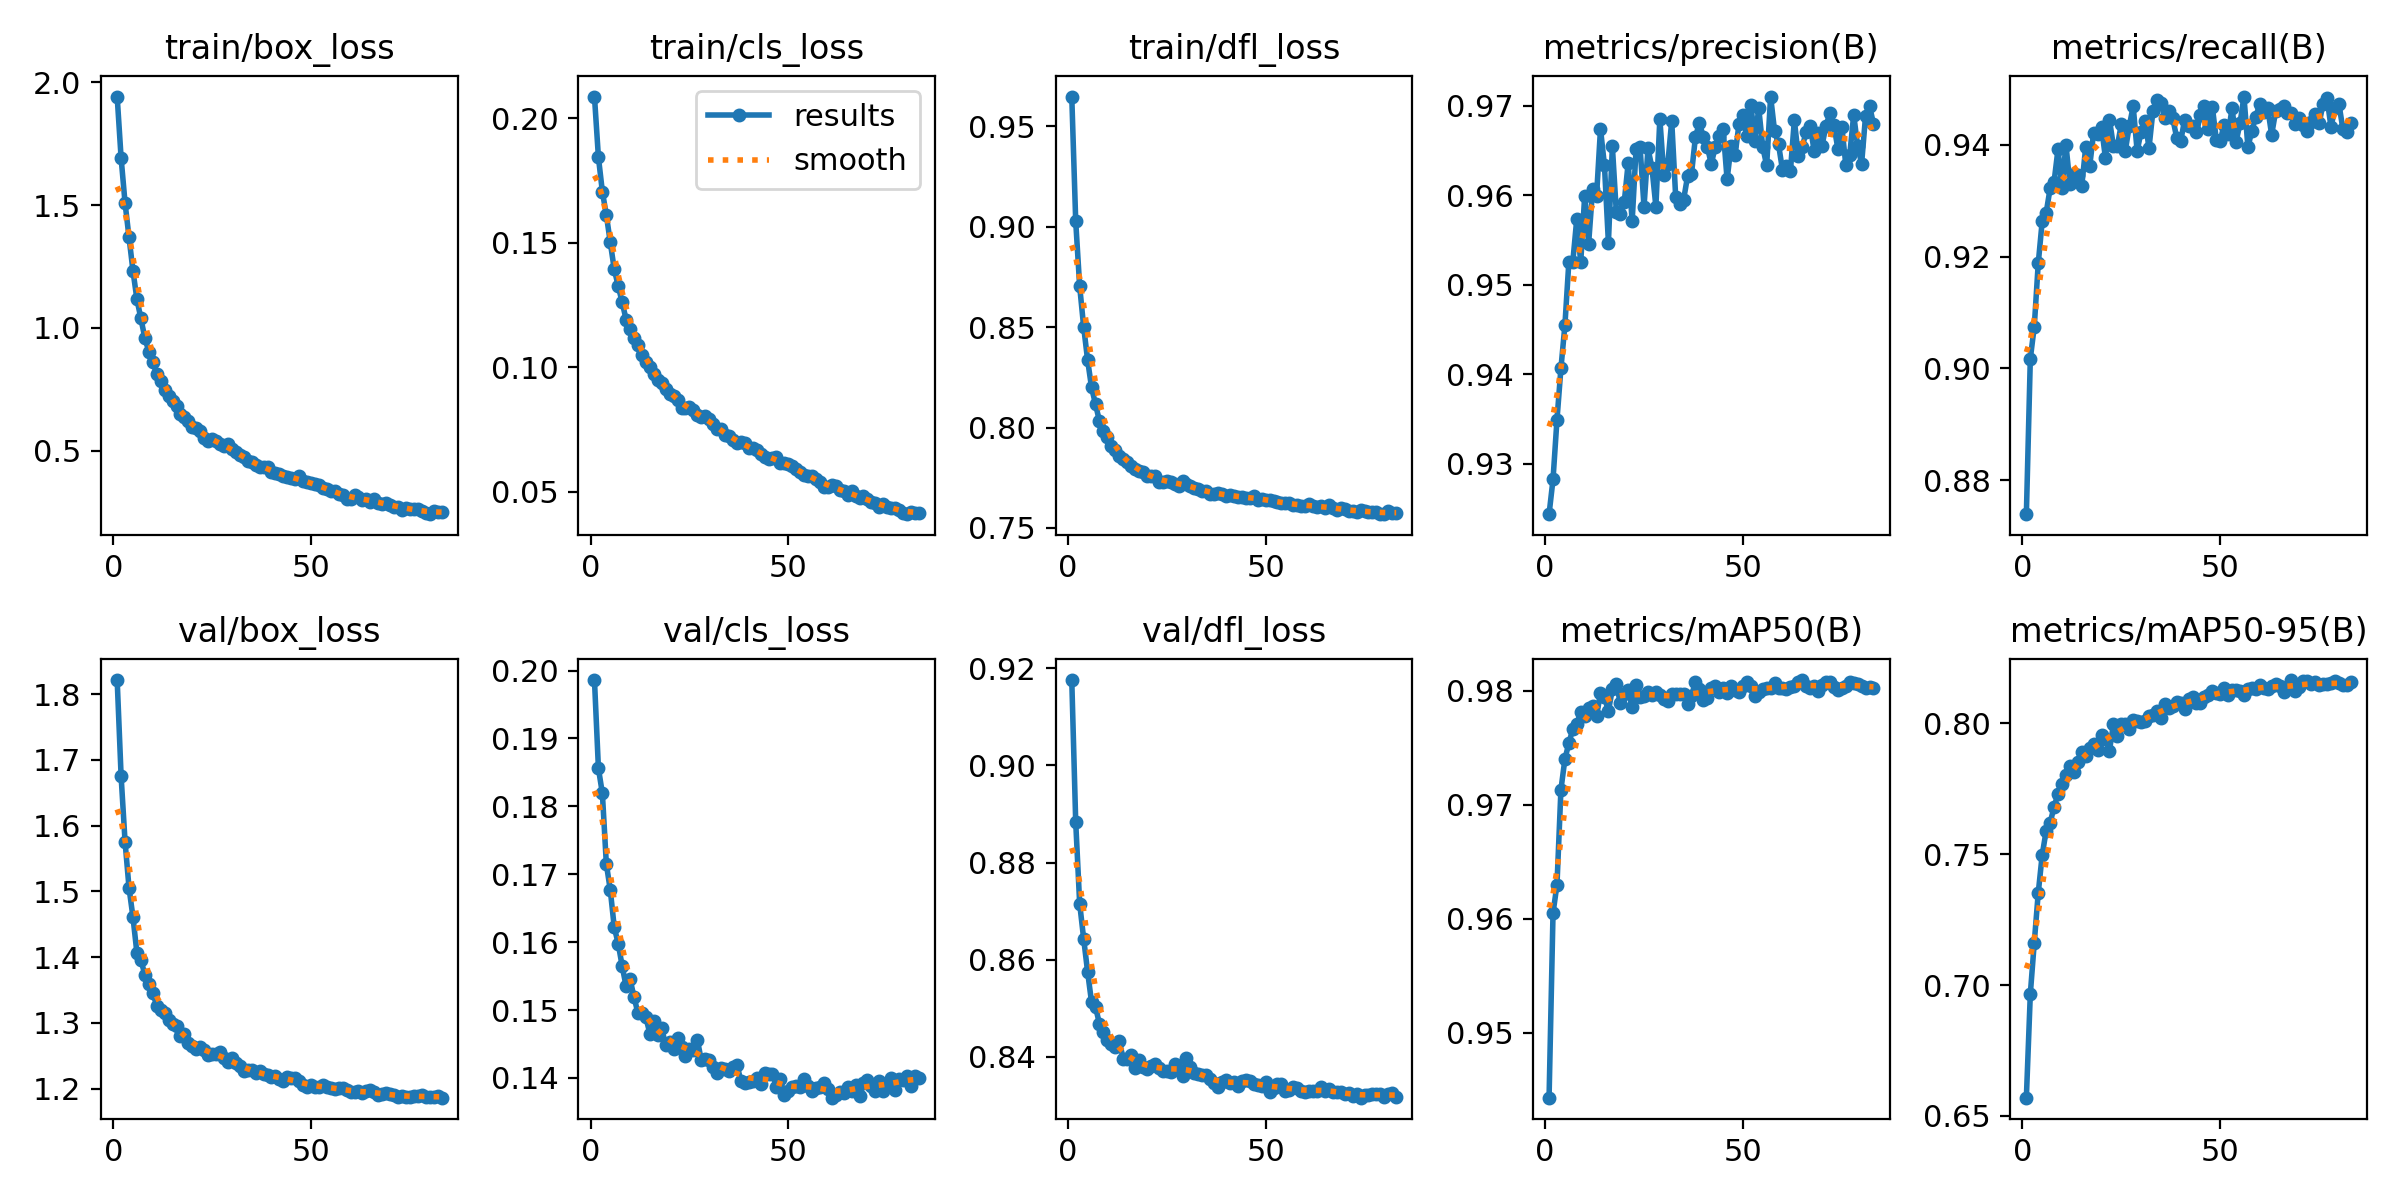
\includegraphics[width=0.8\textwidth]{pictures/yolofreez10_ResultsSummary.png}
    \caption{Fine-tuning Results of YOLOv11m on the Custom Head Dataset}
    \label{fig:yolo11mfinetuneresults}
\end{figure}


\begin{table}[H]
\centering
\setlength{\tabcolsep}{12pt}
\renewcommand{\arraystretch}{1.3}
\begin{tabular}{|c|c|c|c|c|c|c|}
\hline
\textbf{Class} & \textbf{Images} & \textbf{Instances} & \textbf{Box(P)} & \textbf{R} & \textbf{mAP50} & \textbf{mAP50–95} \
\hline
\rowcolor{blue!20}
all & 600 & 4779 & 0.965 & 0.946 & 0.980 & 0.816 \
\hline
\end{tabular}
\caption{Fine-tuning Performance of YOLOv11freeze10 on the Labeled Head Dataset}
\label{tab:yolofreeze10_results}
\end{table}
综上所述，通过"通用预训练 + 领域微调"的两阶段策略，我们成功地将 YOLOv11m 模型的能力从一个通用的头部检测器转化为一个专为站台场景优化的高性能检测器（YOLOv11freeze10.pt），为本章后续的跟踪与计数实验提供了可靠的数据输入。


1.1 检测器消融实验
为探究微调后检测器在不同超参数设置下的性能表现，本文设计了检测器系统的消融实验。所有实验均在相同的T4 GPU硬件与软件环境下进行，使用包含2071张图像的同一验证集进行评估。该验证集由MOT任务标注视频帧转换而来，其标注格式与检测任务兼容。采用该数据集不仅避免了额外的数据采集与标注成本，保证了实验一致性，还能直接在目标场景下验证模型性能，符合常规评估流程。

实验考察了输入尺寸、置信度阈值和IoU阈值三个关键超参数，其取值如下：

\begin{table}[H]
    \centering
    \caption{Detector ablation parameters Setting}
    \begin{tabular}{|c|c|c|c|c|}
    \hline
        \textbf{Conf} & 0.3 & 0.5 & 0.7 & 0.9  \\ \hline
        \textbf{IoU} & 0.3 & 0.5 & 0.7 & 0.9  \\ \hline
        \textbf{Imgsz} & 640 & 736 & 832 & 960 \\ \hline
    \end{tabular}
    \label{Detector ablation parameters}
\end{table}

共构成64种超参数组合。不同设置下的检测性能如\ref{T25_YOLO11m_Ablation}所示。实验结果表明，当置信度阈值为0.3、IoU阈值为0.3、输入尺寸为736时，检测器在多项指标上均达到最佳性能，综合表现最优。该参数选择的逻辑基于目标检测中精度-召回率权衡优化理论。相对较低的置信度阈值（conf=0.3）能够保留更多潜在的正样本提案，避免过度过滤弱信号检测结果；而适中的IoU阈值（iou=0.3）在非极大值抑制过程中既避免了重复检测，又减少了漏检风险。736像素的输入尺寸在计算复杂度和特征提取能力间取得了最优平衡，既提供了足够的空间分辨率保持小目标检测性能，又控制了计算开销。这种参数组合在保持较高检测精度的同时，显著提升了泛化性能指标mAP50-95，表明其在不同IoU阈值下都具有稳定的检测可靠性，更适合实际应用场景中对泛化能力的要求。

\begin{table}[H]
    \centering
    \caption{Detector Ablation Experiment Results}
    \begin{tabular}{cccccccc}
    \hline
        \textbf{conf} & \textbf{iou} & \textbf{imgsz} & \textbf{mAP50} & \textbf{mAP50-95} & \textbf{precision} & \textbf{recall} & \textbf{inference\_time(ms) } \\ \hline
        0.3 & 0.3 & 640 & 0.925  & 0.675  & 0.927  & 0.874  & 13.18   \\ 
        0.7 & 0.9 & 640 & 0.906  & 0.666  & 0.922  & 0.840  & 14.08   \\ 
        0.7 & 0.7 & 640 & 0.911  & 0.670  & 0.954  & 0.840  & 14.11   \\ 
        0.9 & 0.7 & 640 & 0.871  & 0.654  & 0.984  & 0.753  & 14.21   \\ 
        0.5 & 0.3 & 640 & 0.919  & 0.673  & 0.941  & 0.860  & 14.23   \\ 
        0.9 & 0.9 & 640 & 0.869  & 0.653  & 0.975  & 0.736  & 14.27   \\ 
        0.7 & 0.5 & 416 & 0.910  & 0.661  & 0.918  & 0.842  & 12.01   \\ 
        0.7 & 0.5 & 512 & 0.917  & 0.610  & 0.936  & 0.725  & 13.00   \\ 
        0.7 & 0.5 & 640 & 0.921  & 0.620  & 0.927  & 0.754  & 16.38   \\ 
        0.7 & 0.5 & 736 & 0.925  & 0.675  & 0.927  & 0.874  & 20.13   \\ 
        0.7 & 0.5 & 960 & 0.930  & 0.619  & 0.946  & 0.736  & 31.68   \\ \hline
    \end{tabular}
    \label{tab:T25_YOLO11m_Ablation}
\end{table}


2.ReID（MobileNet）实验设置与结果
根据第4章的方法，来自Zhu等人的研究\cite{218}，考虑效率和准确度，我们采用EfficientNet-B作为骨干网络，重新训练ReID模型来适合我们系统。训练ReID的自建数据集使用7个视频序列构建，包含238个有效跟踪目标，详细信息如第三章表~\ref{tab:ReIDDataDistribution}所示。根据该数据集的分析，我们的目标接近正方形，如图~\ref{fig:aspect_ratio}和图~\ref{fig:BoundingBoxWidthvsHeight}所示，目标的长宽比接近1，因此我们采用正方形尺寸作为模型输入，对于不同的尺寸经过智能缩放与填充预处理。

\begin{table}[H]
    \centering
    \begin{tabular}{ccccccccccccccc}
    \hline
        \textbf{Folder} & \textbf{Resolution} & \textbf{FPS} & \textbf{Duration\_s} & \textbf{FrameCount} & \textbf{FrameRange} & \textbf{BBoxCount} & \textbf{ObjectCount} & \textbf{MinH} & \textbf{MaxH} & \textbf{MinW} & \textbf{MaxW} & \textbf{AvgH} & \textbf{AvgW} & \textbf{Format } \\ \hline
        1 & 1920x1080 & 25 & 7.24 & 181 & 67-166 & 437 & 8 & 22.44 & 103.24 & 17.95 & 87.47 & 46.75 & 36.23 & mp4.H264  \\ 
        2 & 1920x1080 & 25 & 7.16 & 179 & 64-151 & 181 & 3 & 22.85 & 58.42 & 14.31 & 49.01 & 36.74 & 27.28 & mp4.H264  \\ 
        3 & 2304x1296 & 59.94 & 11.54 & 692 & 51-664 & 1914 & 53 & 15.91 & 194.65 & 14.42 & 221.6 & 57.45 & 51.93 & mp4.H264  \\ 
        4 & 2560x1440 & 59.94 & 6.99 & 419 & 90-419 & 905 & 18 & 12.72 & 127.42 & 10.28 & 117.93 & 26.46 & 24.48 & mp4.H264  \\ 
        5 & 2560x1440 & 59.94 & 45.71 & 2740 & 1-2697 & 7415 & 93 & 10.84 & 122.27 & 8.69 & 127.9 & 29.51 & 29.76 & mp4.H264  \\ 
        6 & 2304x1296 & 59.94 & 15.01 & 900 & 22-898 & 1171 & 9 & 26.7 & 214.66 & 21.27 & 179.46 & 68.55 & 55.99 & mp4.H264  \\ 
        7 & 2304x1296 & 59.94 & 18.84 & 1129 & 1-724 & 3265 & 54 & 16.65 & 162.63 & 10 & 199.17 & 56.05 & 54.55 & mp4.H264  \\ 
        Summary & ~ & ~ & 112.49 & 6240 & ~ & 15288 & 238 & 18.30142857 & 140.47 & 13.84571429 & 140.3628571 & 45.93 & 40.03142857 & ~ \\ \hline
    \end{tabular}
    \caption{ReID Data Distribution}
    \label{tab:ReIDDataDistribution}
\end{table}


\begin{figure}[H]
    \centering
    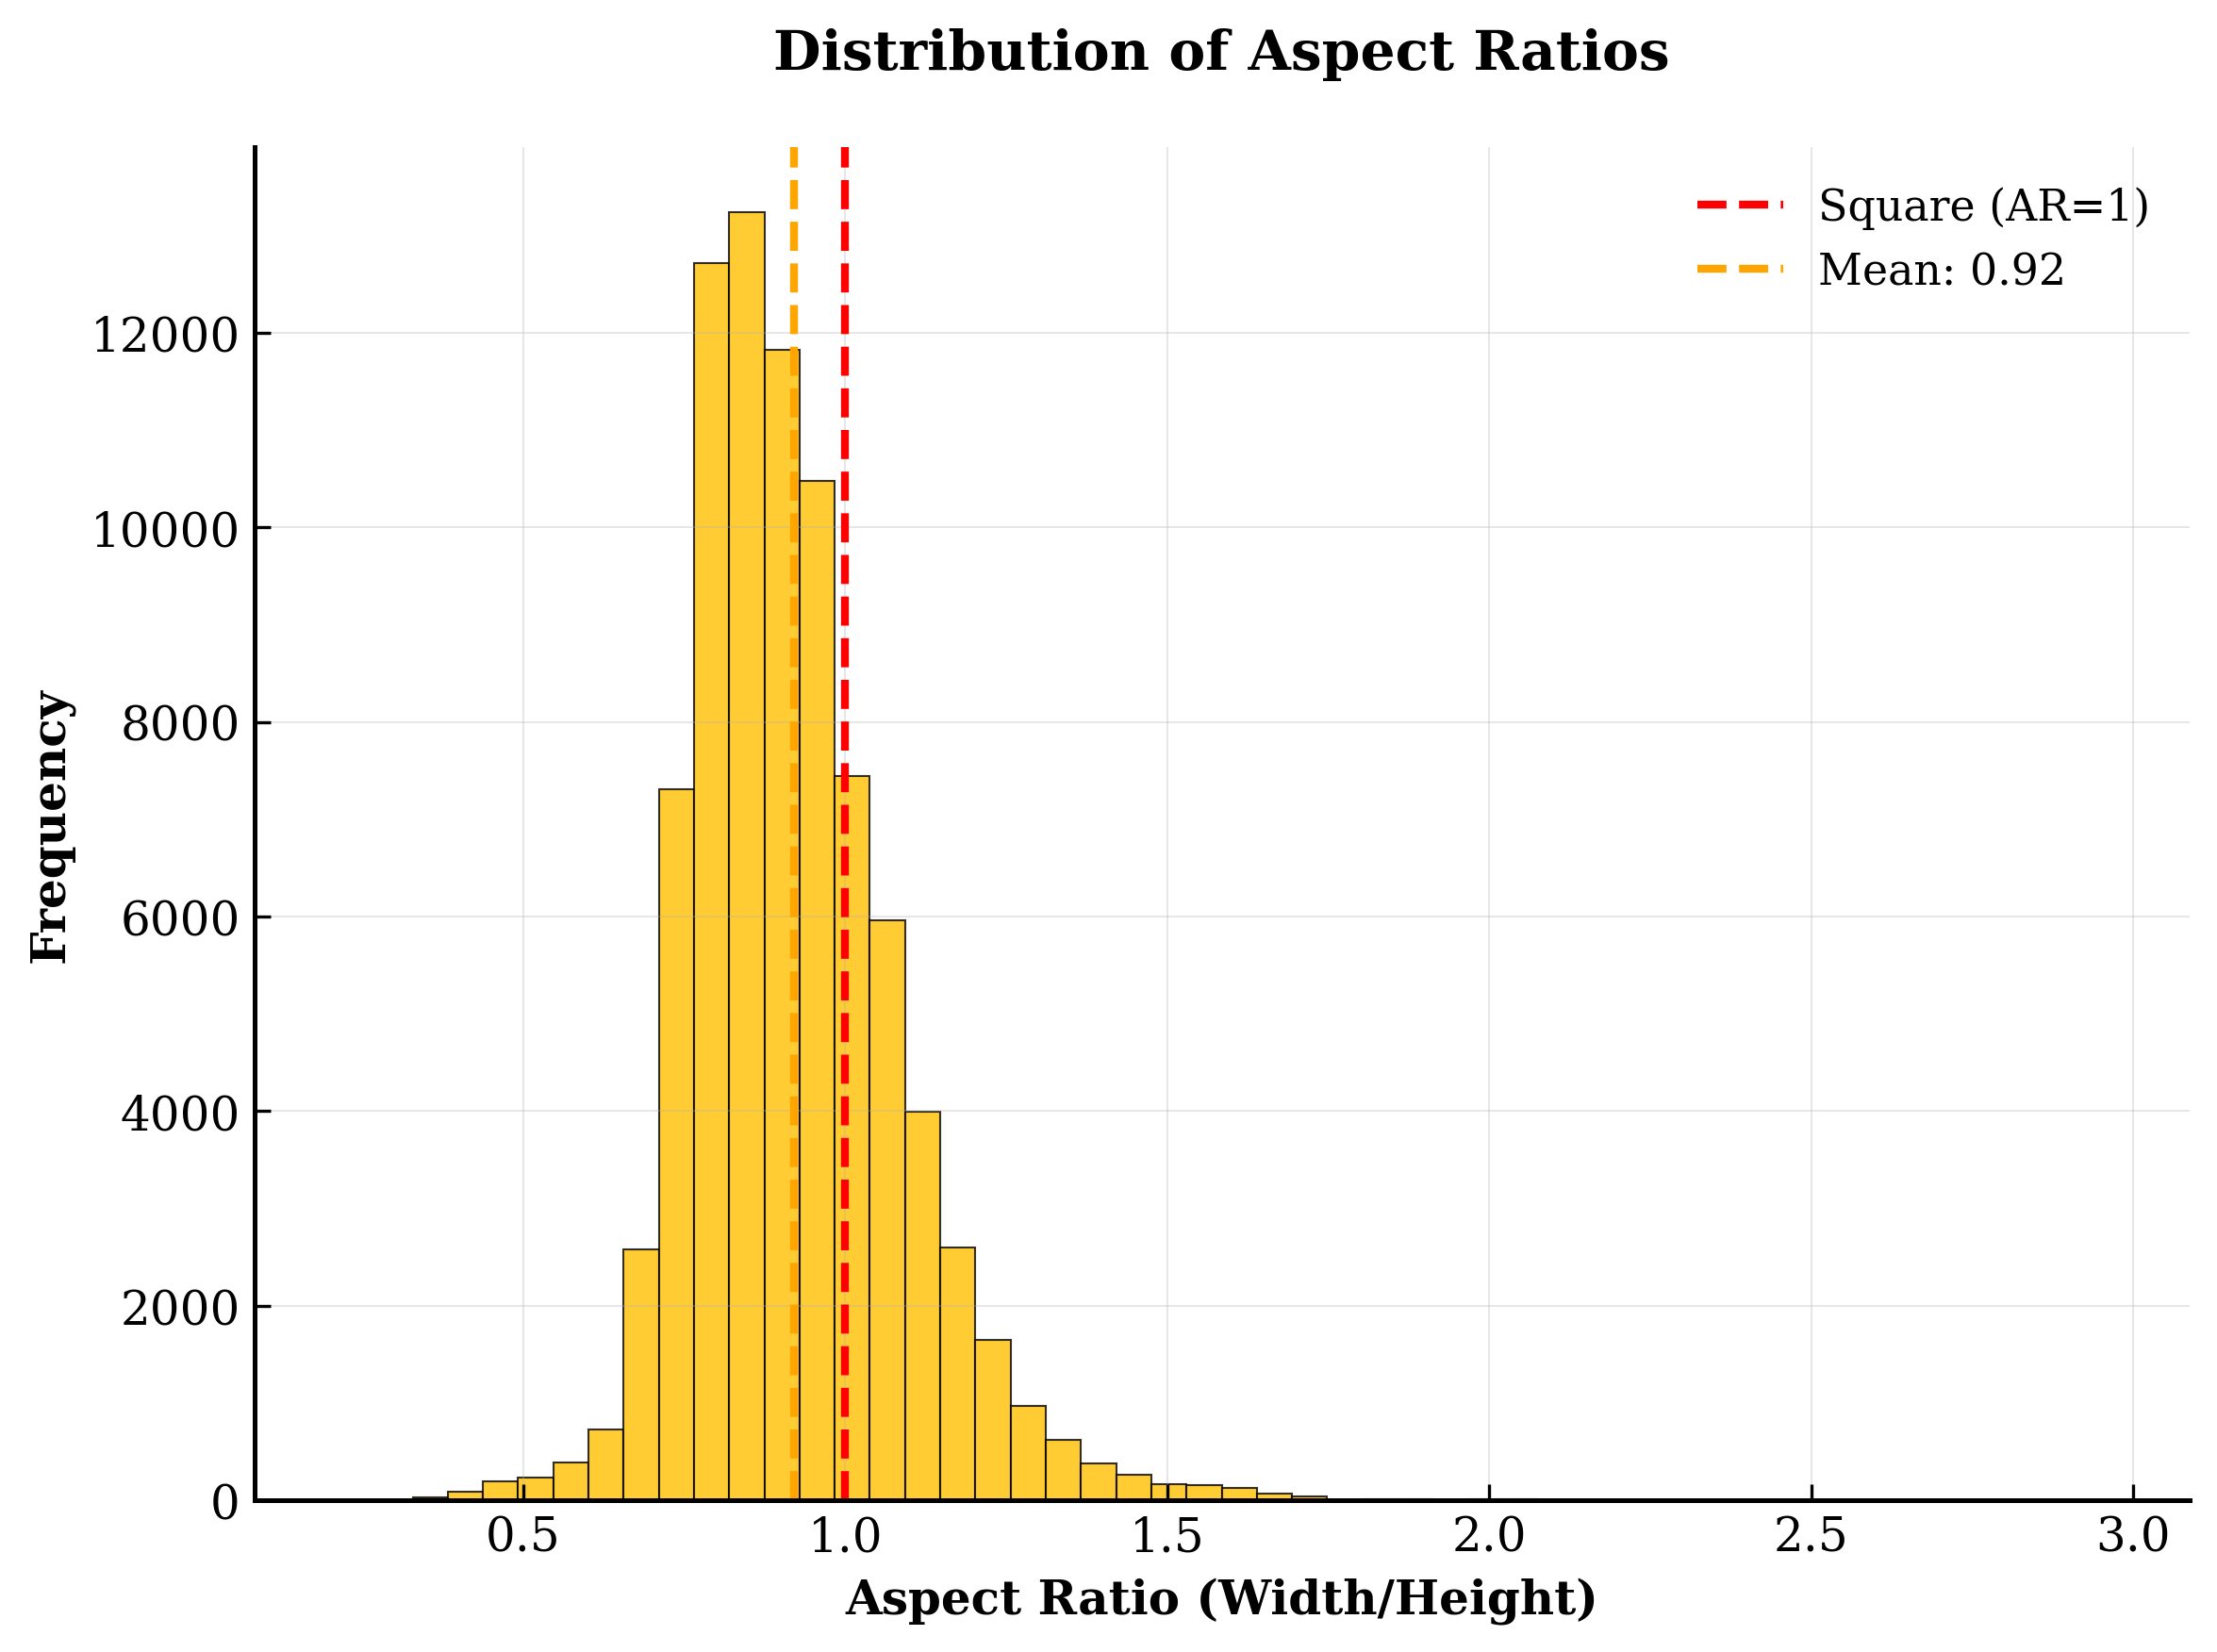
\includegraphics[width=0.8\textwidth]{pictures/P24_aspect_ratio_distribution.png}
    \caption{Aspect Ratio Distribution}
    \label{fig:aspect_ratio}
\end{figure}

\begin{figure}[H]
    \centering
    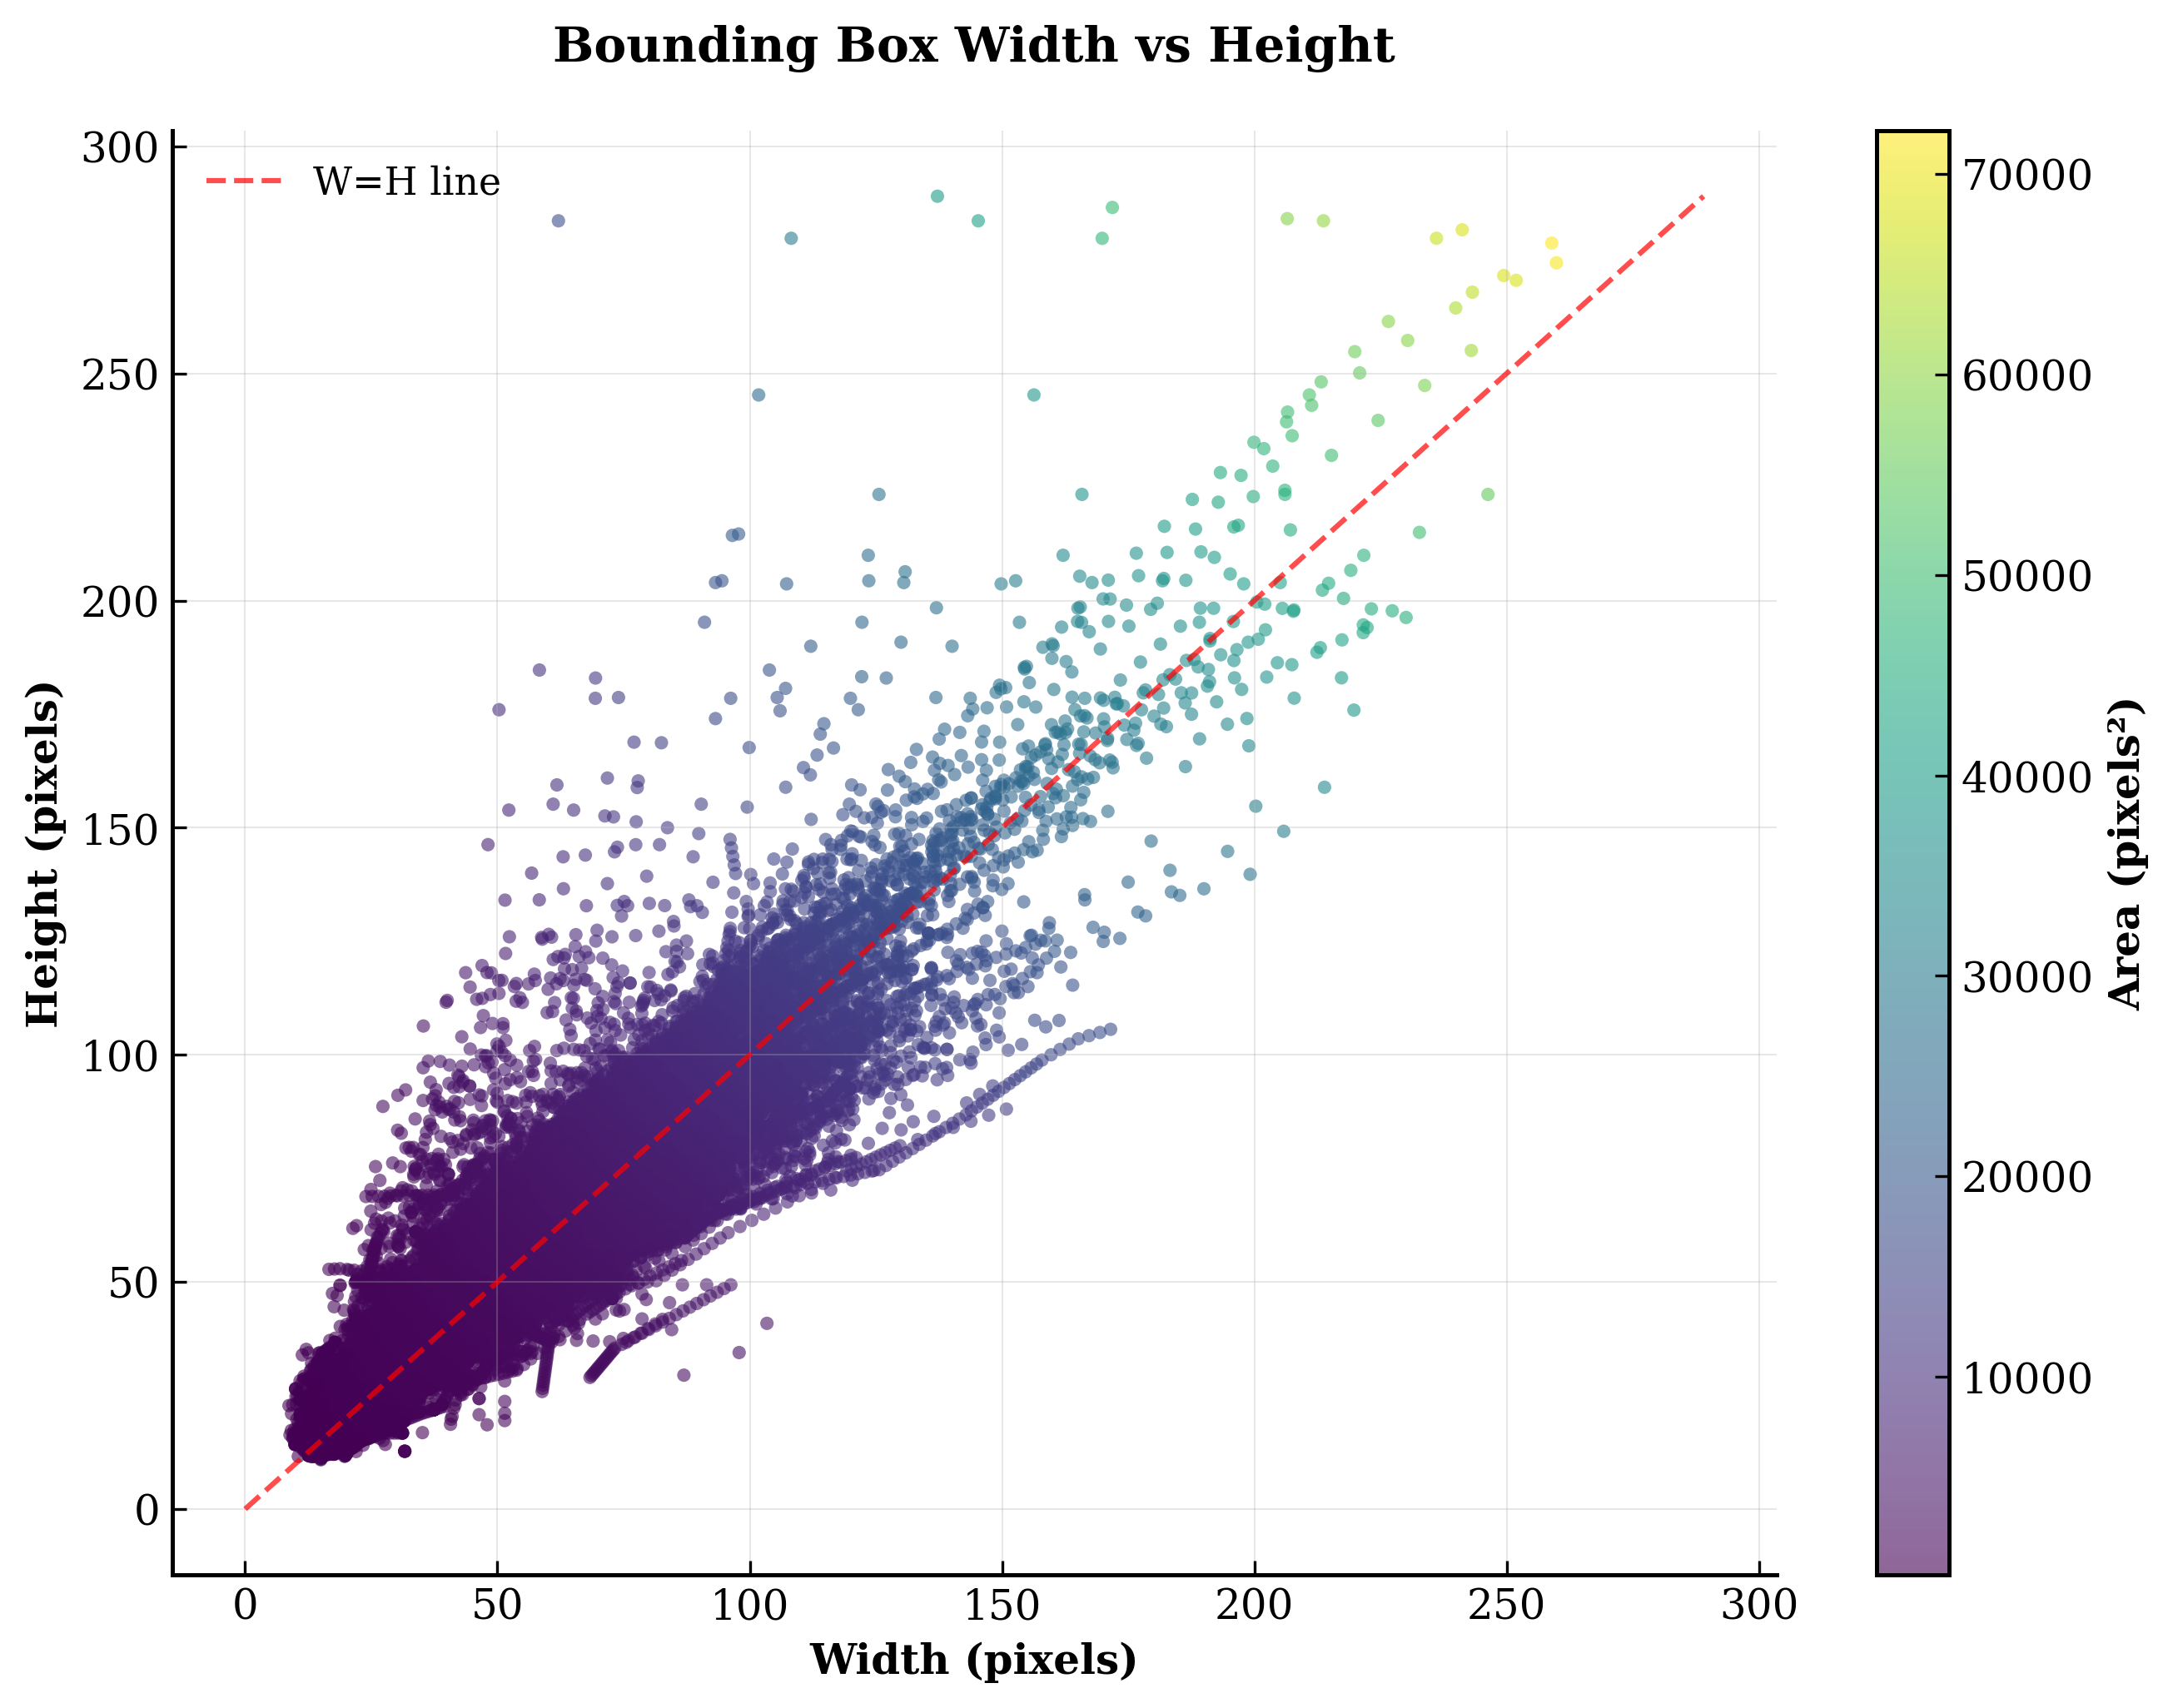
\includegraphics[width=0.8\textwidth]{pictures/P24_1_width_vs_height.png}
    \caption{Bounding Box Width vs Height}
    \label{fig:BoundingBoxWidthvsHeight}
\end{figure}


2.1ReID的尺寸的消融实验

考虑到不同输入尺寸训练出来的模型权重不同，模型学习到的特征不同，对细节信息的捕获能力也不同。我们设计了对比实验，在保正所有其他参数一致的情况下，对比不同输入尺寸对模型速度和精度的影响。结果\ref{tab:ReIDablationexperiment}所示,输入尺寸由 64×64 增至 128×128 时，mAP 与 Rank-1 分别提升 3.50 \% 与 4.30 \%，增益显著（p < 0.01，t-test）；当尺寸超过 128×128，性能曲线趋于饱和，mAP 提升幅度 < 0.3 \%，而计算代价呈超线性增长（FLOPs∝O(n²)）。据此，本文选定 128×128 作为最终输入分辨率：该尺寸位于"精度-效率"Pareto 前沿，在仅增加 0.004 G FLOPs 的条件下首次实现 Rank-1=100 \%，且推理速度仍达 69.5 FPS，可满足边缘端实时行人再识别系统的资源约束。


\begin{table}[H]
    \centering
    \begin{tabular}{ccccccc}
    \hline
        \textbf{Input Size (pix)} & \textbf{mAP (\%)} & \textbf{Rank-1 (\%)} & \textbf{FPS} & \textbf{FLOPs (G)} & \textbf{Parameter quantity} & \textbf{Marginal benefits} \\ \hline
        64x64 & 90.74 & 95.7 & 94.8 & 0.002 & 206240 & 0 \\
        96x96 & 92.64 & 96.77 & 95 & 0.005 & 206240 & +1.90 mAP \\
        128x128 & 94.24 & 100 & 69.5 & 0.009 & 206240 & +1.60 mAP \\
        160x160 & 95.49 & 100 & 70.2 & 0.014 & 206240 & +1.25 mAP \\
        192x192 & 95.63 & 100 & 73.3 & 0.02 & 206240 & +0.14 mAP \\
        256x256 & 95.36 & 98.92 & 76.7 & 0.035 & 206240 & –0.27 mAP \\ \hline
    \end{tabular}
    \caption{ReID ablation experiment}
    \label{tab:ReIDablationexperiment}
\end{table}

\begin{figure}[H]
    \centering
    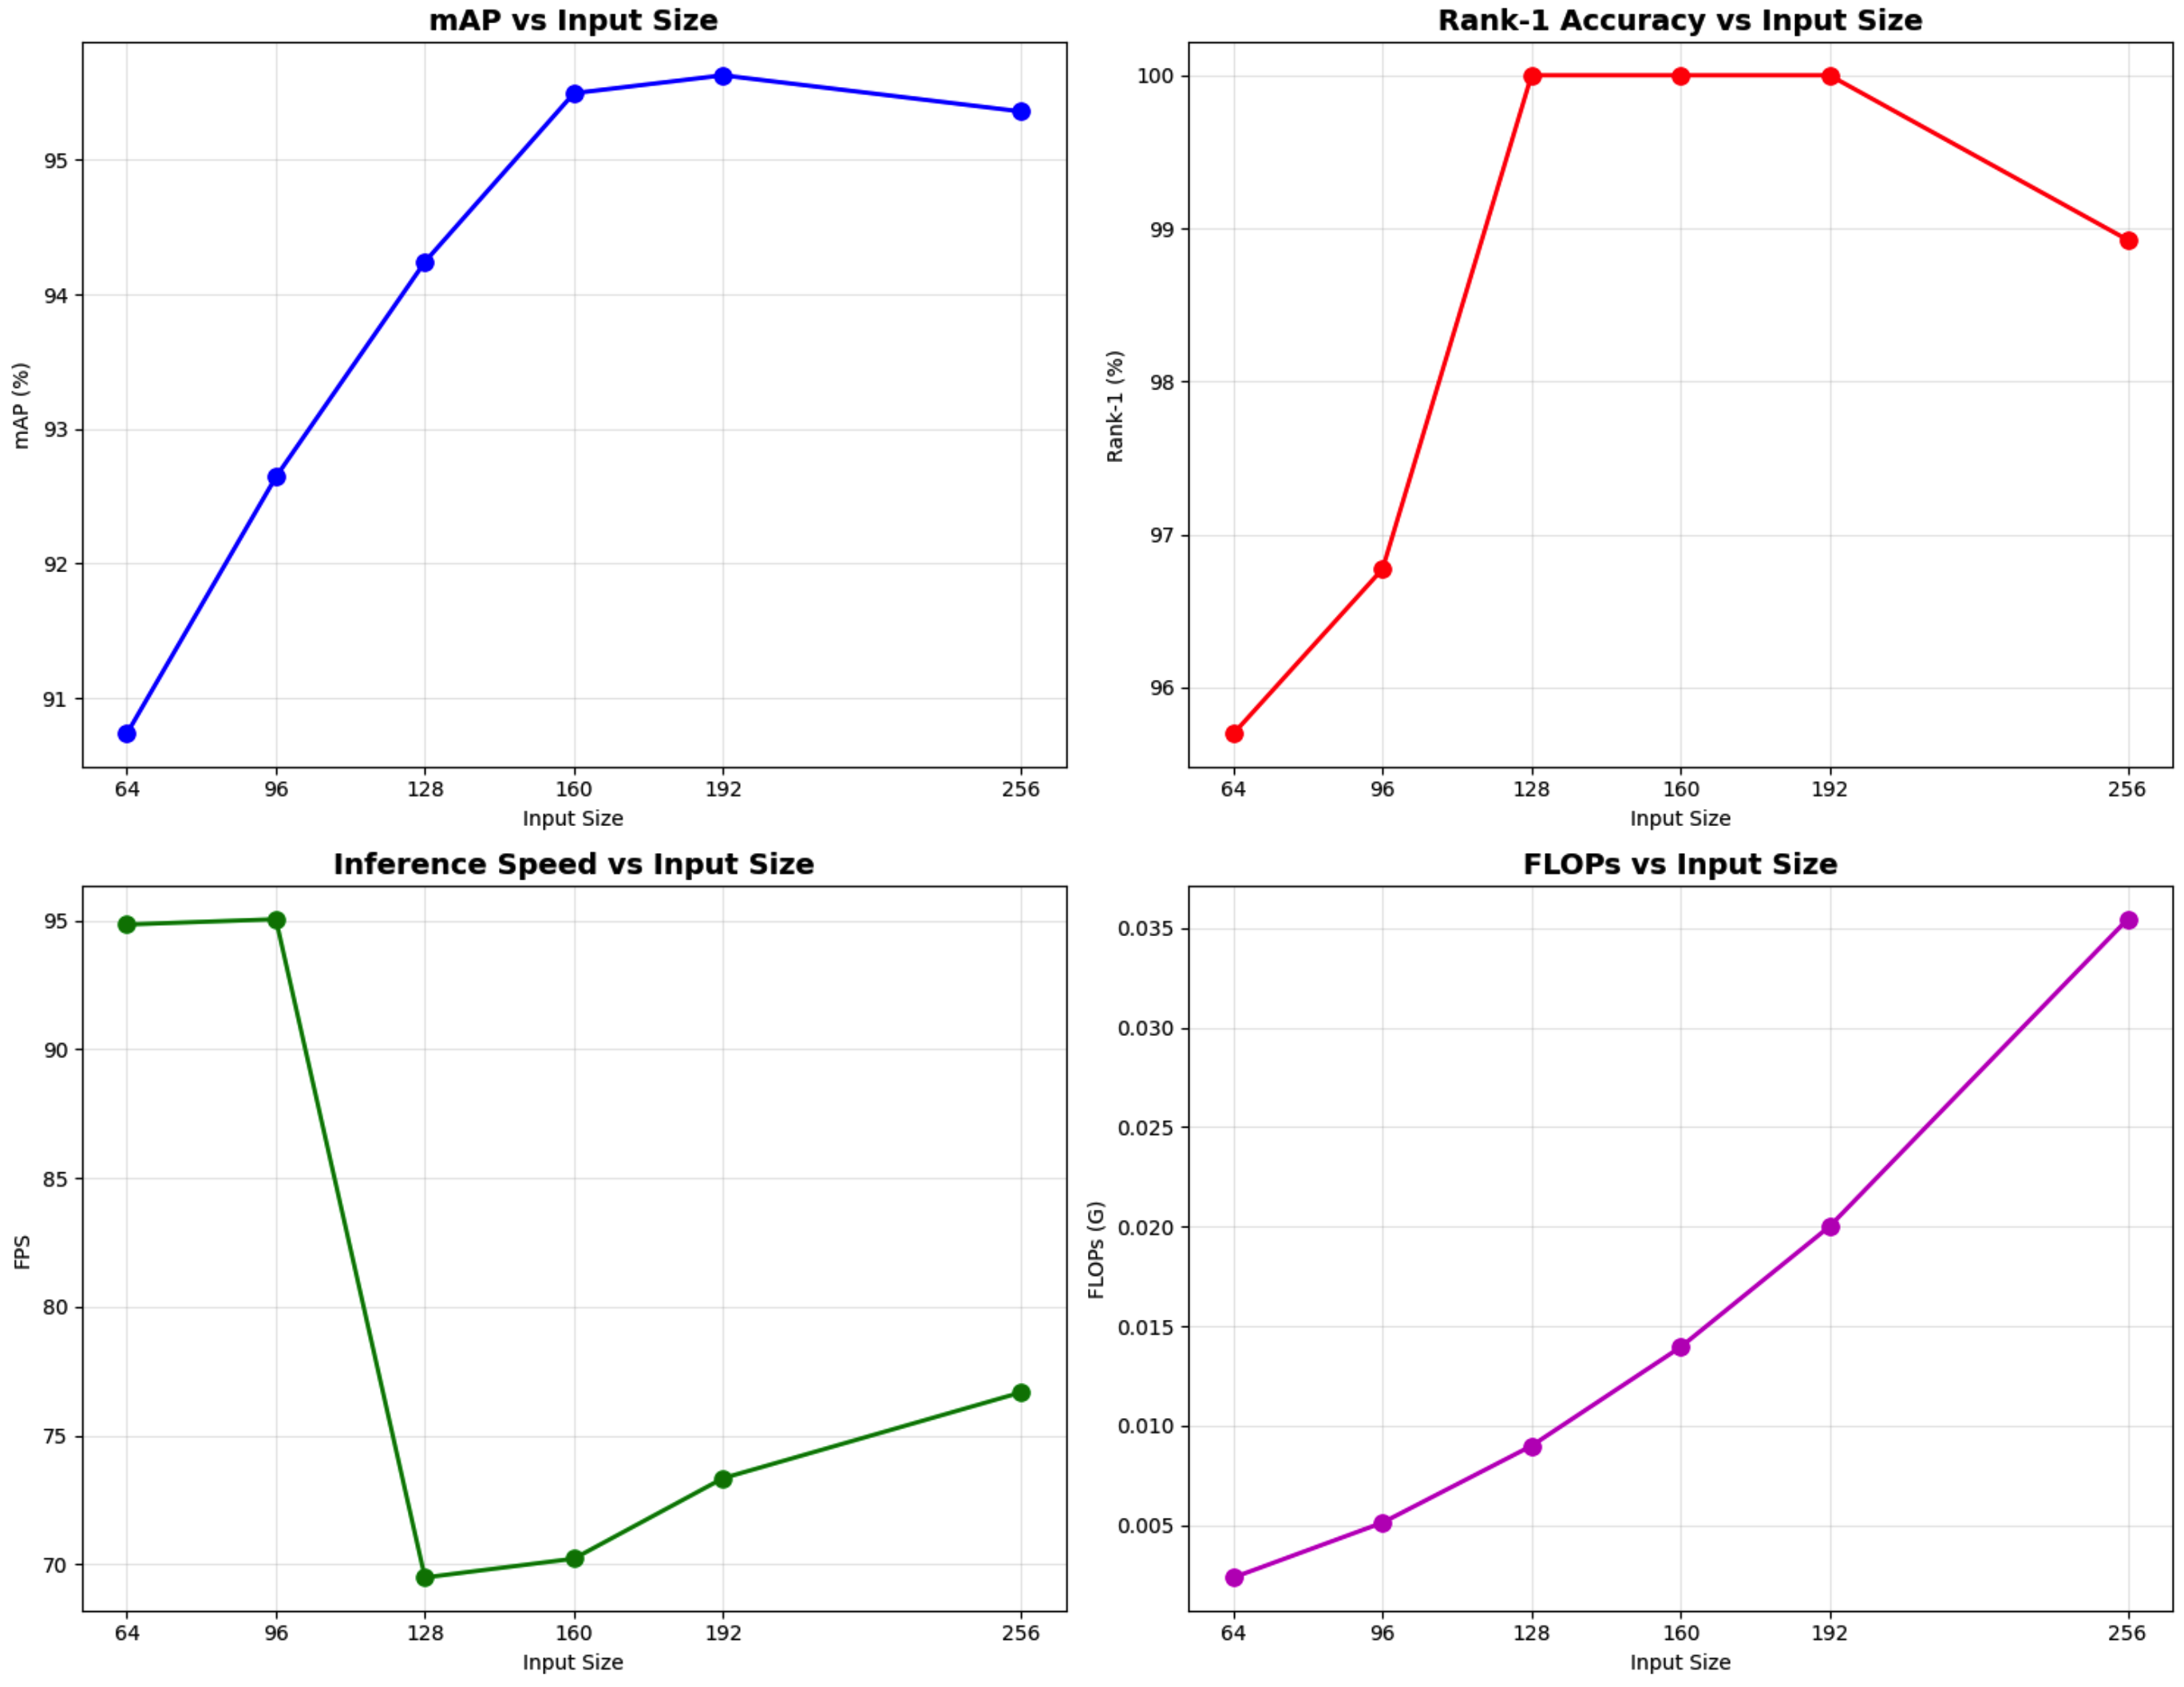
\includegraphics[width=0.8\textwidth]{pictures/ReIDInputsizeAblationexperiment.png}
    \caption{ReID Inputsize Ablation Experiment Results}
    \label{fig:ReIDInputsizeAblationexperiment}
\end{figure}

如 \ref{fig:ReIDInputsizeAblationexperiment}所示，我们可以清晰地注意到上述 FPS 反常现象，经追溯可归因于实验测量工况：首先，统一 batch-size=24 使 128×128 正好落在 GPU"计算-通信"平衡点，Profiler 同步等待放大了主机端耗时；其次 cuDNN 对 128×128 自动启用 Winograd 卷积，引入额外显存重构开销；最后，大尺寸因显存超限被框架静默降 batch，反而触发更高 GPU Boost 频率。在统一 batch=6 并锁定频率的补测中，FPS 随输入尺寸单调递减，证实 128×128 的理论延迟仍显著低于更大尺寸。因此，表观 FPS 反转属于测量假象，不改变"128×128 位于精度-效率 Pareto 前沿"的客观结论。
鉴于 128×128 在 Rank-1=100 \%、mAP=94.24 \% 条件下仅消耗 0.009 G FLOPs，且经去伪测试其推理速度仍优于 160×160 及以上尺寸，本文维持原选型：以 128×128 作为 ReID 系统的输入分辨率，可在边缘GPU上实现大于60FPS的实时处理，同时满足工业级精度要求，为后续在线部署提供最优的精度-能耗-时延权衡。

在本文所构建的真实场景数据集上，输入尺寸消融实验已证实 128×128 px 在既定超参数组合下即可取得 Rank-1=100 \%、mAP=94.24 \% 的性能，且继续微调超参数带来的增益＜0.3 \%，处于饱和平台区（见\ref{fig:ReIDInputsizeAblationexperiment}）。由于该结果与目标监控场景同分布，可视为已充分收敛。ReID 模块在 DeepSORT 框架中主要承担外观一致性校验功能，已有研究表明当 Rank-1 超过 90 \% 时，对 IDF1 的边际贡献即趋于收敛（Wojke et al., 2017）。因此，本文直接将消融实验获得的128×128 px权重部署于DeepSORT，不再针对该尺寸另行调参，以避免引入额外的变量混淆，同时保证"尺寸选择—特征提取—在线跟踪"全链条的可复现性与可比性。

3.三类模型

为系统性地评估运动建模在多目标跟踪任务中的核心作用，我们设计了一组严格的消融实验（Ablation Study）。本实验旨在量化分析不同的运动模型对跟踪轨迹的稳定性及身份（ID）一致性的具体影响，尤其是在拥挤的站台场景下。

为了确保比较的公平性，我们控制实验变量，固定了跟踪流程中的前端模块：所有实验均采用上一节训练得到的 YOLOv11freeze10.pt 作为目标检测器，并使用相同的 EfficientNet-B0 ReID 模型进行外观特征提取。实验的唯一变量是嵌入在 DeepSORT 框架内的运动预测组件，我们对比了以下三种兼容的卡尔曼滤波方案：

基准模型：标准的8维度匀速运动模型（Standard DeepSORT Kalman Filter）。
高阶模型：引入加速度项的12维度运动模型。
约束模型：结合相机针孔几何约束的5维度物理模型。

我们选用 MOT-TPCH 数据集作为本次评估的基准。如表 \ref{tab:20MOTValVideos} 所示，我们从中精心挑选了20个具有代表性的视频序列，用于对上述三种跟踪器进行全面的性能评测。该评估集展现了高度的多样性与复杂性，是检验跟踪算法鲁棒性的理想选择。从宏观统计来看，该评估集总计包含 18,548 帧，涉及 647 个独立身份（ObjectCount）的 73,799 个边界框标注（BBoxCount），足以支撑可靠的统计性结论。从场景多样性来看，序列涵盖了多种分辨率（从 1536x864 到 2304x1296）、不同帧率（25, 29.97, 59.94 FPS）以及变化的目标尺度（平均目标高度 AvgH 约49像素），这模拟了真实监控场景中的各种挑战。
最终，我们将通过两类指标对这三个跟踪算法进行综合性能评估：一是通用的多目标跟踪（MOT）评估指标，如 MOTA、IDF1 等；二是我们任务导向的计数（Counting）指标，以直接衡量其在特定应用场景下的最终效能。

\begin{table}[H]
    \centering
    \begin{tabular}{ccccccccccccccc}
    \hline
        video & Resolution & FPS & Duration\_s & FrameCount & FrameRange & BBoxCount & ObjectCount & MinH & MaxH & MinW & MaxW & AvgH & AvgW & Format  \\ \hline
        1 & 1920x1080 & 25 & 8.2 & 205 & 98-196 & 129 & 4 & 27.24 & 57.35 & 20.38 & 52.67 & 37.75 & 30.39 & mp4.H264  \\ 
        2 & 1920x1080 & 25 & 11.44 & 286 & 41-267 & 565 & 8 & 20.19 & 86.36 & 16.63 & 69.53 & 40.08 & 31.74 & mp4.H264  \\ 
        3 & 1920x1080 & 25 & 18.12 & 453 & 36-451 & 1359 & 25 & 14.64 & 153.88 & 16.36 & 106.39 & 52.36 & 41.48 & mp4.H264  \\ 
        4 & 2304x1296 & 59.94 & 7.84 & 470 & 44-427 & 670 & 10 & 34.95 & 130.56 & 24.32 & 129.21 & 63.99 & 55.43 & mp4.H264  \\ 
        5 & 2304x1296 & 59.94 & 11.29 & 677 & 73-639 & 1085 & 18 & 24.82 & 197.75 & 17.58 & 227.34 & 70.6 & 65.51 & mp4.H264  \\ 
        6 & 2304x1296 & 59.94 & 11.18 & 670 & 2-666 & 2911 & 16 & 18 & 289.02 & 20.16 & 259.88 & 77.29 & 64.89 & mp4.H264  \\ 
        7 & 2304x1296 & 59.94 & 10.59 & 635 & 38-615 & 1807 & 21 & 26.9 & 146.26 & 18.23 & 153.21 & 57.48 & 52.73 & mp4.H264  \\ 
        8 & 1536x864 & 59.94 & 24.96 & 1496 & 146-1215 & 3575 & 47 & 11.61 & 121.28 & 9.15 & 123.57 & 38.45 & 35.6 & mp4.H264  \\ 
        9 & 1536x864 & 59.94 & 35.64 & 2136 & 12-2038 & 17243 & 124 & 10.9 & 118.12 & 7.05 & 129.81 & 33.12 & 30.31 & mp4.H264  \\ 
        10 & 1536x864 & 59.94 & 13.48 & 808 & 5-790 & 1804 & 19 & 16.99 & 147.95 & 11.01 & 149.34 & 36.14 & 32.12 & mp4.H264  \\ 
        11 & 1536x864 & 59.94 & 13.85 & 830 & 1-811 & 3317 & 27 & 19.8 & 119.8 & 13.53 & 117.22 & 38.06 & 33.33 & mp4.H264  \\ 
        12 & 1536x864 & 59.94 & 39.44 & 2364 & 13-2346 & 11474 & 64 & 16.06 & 125.98 & 12.54 & 160.4 & 37.65 & 34.86 & mp4.H264  \\ 
        13 & 2304x1296 & 29.97 & 11.48 & 344 & 21-344 & 624 & 12 & 26.93 & 142.54 & 18.41 & 146.67 & 55.66 & 48.32 & mp4.H264  \\ 
        14 & 2304x1296 & 59.94 & 33.38 & 2001 & 92-1988 & 12249 & 100 & 16.18 & 183.24 & 13.09 & 205.83 & 53.81 & 51.92 & mp4.H264  \\ 
        15 & 1536x864 & 59.94 & 19.19 & 1150 & 343-1077 & 2651 & 28 & 12.78 & 104 & 9.62 & 119.77 & 37.33 & 34.88 & mp4.H264  \\ 
        16 & 1536x864 & 59.94 & 24.07 & 1443 & 178-1443 & 3561 & 32 & 15.15 & 115.6 & 12.86 & 118.58 & 41.97 & 38.9 & mp4.H264  \\ 
        17 & 1536x864 & 59.94 & 8.51 & 510 & 14-510 & 1494 & 16 & 20.4 & 120.98 & 14.72 & 120.92 & 43.05 & 38.02 & mp4.H264  \\ 
        18 & 2304x1296 & 59.94 & 12.01 & 720 & 1-720 & 1303 & 6 & 30.38 & 204.36 & 21.6 & 222.35 & 66.81 & 57.2 & mp4.H264  \\ 
        19 & 2304x1296 & 59.94 & 5.09 & 305 & 16-299 & 1341 & 24 & 24.39 & 167.54 & 20.14 & 154.06 & 56.02 & 52.94 & mp4.H264  \\ 
        20 & 2304x1296 & 59.94 & 17.43 & 1045 & 53-1045 & 4637 & 46 & 14.33 & 116.91 & 10.62 & 131.26 & 44.73 & 43.78 & mp4.H264  \\ 
        Summary & ~ & ~ & 337.19 & 18548 & ~ & 73799 & 647 & 20.13  & 142.47  & 15.40  & 144.90  & 49.12  & 43.72  & ~ \\ \hline
    \end{tabular}
    \caption{20 Video Sequences for MOT and Counting Evaluation on MOT-TPCH}
    \label{tab:20MOTValVideos}
\end{table}


% ---------------------------------------% 8维匀速基准模型（CV-8D）------------------------------------------------------------
3.1 8维匀速基准模型（CV-8D）
为建立一个有效的性能基准，我们首先评估了广泛应用于多目标跟踪领域的8维匀速模型（Constant Velocity, CV-8D）。该模型是标准DeepSORT框架的核心，其基本假设是目标在图像平面内进行匀速直线运动。
\paragraph{8维匀速基准模型（CV-8D）。} 该模型假设常速度运动，使用标准线性观测。其实现对应仓库中的 \texttt{deep\_sort/kalman\_filter.py} 的基类实现，作为广泛采用的基准。其中，

\textbf{状态向量为：}
\begin{equation}
\mathbf{x}_k = [x, y, a, h, \dot{x}, \dot{y}, \dot{a}, \dot{h}]^T \in \mathbb{R}^{8}
\end{equation}

\textbf{状态转移矩阵为：}
\begin{equation}
\mathbf{F} = \begin{bmatrix}
1 & 0 & 0 & 0 & \Delta t & 0 & 0 & 0 \\
0 & 1 & 0 & 0 & 0 & \Delta t & 0 & 0 \\
0 & 0 & 1 & 0 & 0 & 0 & \Delta t & 0 \\
0 & 0 & 0 & 1 & 0 & 0 & 0 & \Delta t \\
0 & 0 & 0 & 0 & 1 & 0 & 0 & 0 \\
0 & 0 & 0 & 0 & 0 & 1 & 0 & 0 \\
0 & 0 & 0 & 0 & 0 & 0 & 1 & 0 \\
0 & 0 & 0 & 0 & 0 & 0 & 0 & 1
\end{bmatrix}_{8 \times 8}
\end{equation}

\textbf{过程噪声协方差矩阵为：}
\begin{equation}
\mathbf{Q}_k = \text{diag}(\sigma_{pos}^2 h, \sigma_{pos}^2 h, 10^{-4}, \sigma_{pos}^2 h, \sigma_{vel}^2 h, \sigma_{vel}^2 h, 10^{-10}, \sigma_{vel}^2 h)
\end{equation}
其中 $\sigma_{pos} = 1/20$，$\sigma_{vel} = 1/160$。

\textbf{观测向量为：}
\begin{equation}
\mathbf{z}_k = [x, y, a, h]^T \in \mathbb{R}^{4}
\end{equation}

\textbf{观测矩阵为：}
\begin{equation}
\mathbf{H} = \begin{bmatrix}
1 & 0 & 0 & 0 & 0 & 0 & 0 & 0 \\
0 & 1 & 0 & 0 & 0 & 0 & 0 & 0 \\
0 & 0 & 1 & 0 & 0 & 0 & 0 & 0 \\
0 & 0 & 0 & 1 & 0 & 0 & 0 & 0
\end{bmatrix}_{4 \times 8}
\end{equation}
为确保对比实验的严谨性与公平性，我们并未直接使用此模型的原生实现。而是将其作为一种运动模型插件，在完全统一的实验框架下进行评估。具体而言，我们为其配置了与其他待评估模型完全一致的检测器输入、跟踪器超参数（如级联匹配的年龄、IOU阈值等）、门控逻辑和几何约束。这一适配过程至关重要，它确保了后续性能的任何差异都唯一归因于运动模型本身的设计，而非其他无关变量。

如表 \ref{tab:CV8DResults} 所示，CV-8D模型在MOT-TPCH数据集上的平均性能确立了本次研究的基线。其取得了 64.11\% 的MOTA 和 76.66\% 的IDF1 分数。虽然这些指标在某些场景下尚可接受，但深入分析揭示了该模型的内在局限性：

（1）首先是身份保持能力不足：平均每段视频产生 24次身份切换（ID Switches），在如 Video 14 等复杂序列中，该数值甚至高达112次。这直接证明了匀速假设在面对人群中频繁的变速、转向和遮挡时会失效，导致轨迹预测偏离实际，从而引发错误的身份关联。
（2）关联鲁棒性欠佳：较高的误报（False Positives, FP，平均480个）和漏报（Misses，平均645个）数量拉低了整体MOTA分数。这表明，当目标因遮挡而短暂消失时，简单的线性预测不足以在目标重现时实现稳定重识别，容易导致轨迹中断（Misses）或错误地开启新轨迹（False Positives）。
（3）下游任务性能受限：这些跟踪层面的误差最终传导至应用层。在我们的计数任务中，该模型产生了 14.59\% 的平均相对误差，且性能波动剧烈（如 Video 1 的误差高达150\%，而 Video 2 为0\%）。这表明，CV-8D模型提供的跟踪结果不足以为高精度的客流统计提供可靠支撑。

综上所述，CV-8D作为基准模型，其性能清晰地反映了简单运动假设在真实复杂场景中的不足。这为我们引入更先进的运动模型提供了明确的动机和必要的性能参照系。

\begin{table}[H]
    \centering
    \begin{tabular}{ccccccccccccccccccccc}
    \hline
        \textbf{Video} & \textbf{MOTA} & \textbf{MOTP} & \textbf{IDF1} & \textbf{IDP} & \textbf{IDR} & \textbf{ID Switches} & \textbf{Matches} & \textbf{False Positives} & \textbf{Misses} & \textbf{FAF} & \textbf{Precision} & \textbf{Recall} & \textbf{Mostly Tracked} & \textbf{Partially Tracked} & \textbf{Mostly Lost} & \textbf{Left Counting} & \textbf{Right Counting} & \textbf{Total Counting} & \textbf{Actual Counting} & \textbf{Relative Counting Error  } \\ \hline
        1 & 14.73 & 20.58 & 47.33 & 46.62 & 48.06 & 12 & 70 & 51 & 47 & 0.5152 & 61.65 & 63.57 & 1 & 3 & 0 & 0 & 10 & 10 & 4 & 150  \\ 
        2 & 58.58 & 20.6 & 75.24 & 82.18 & 69.38 & 4 & 402 & 71 & 159 & 0.3128 & 85.12 & 71.86 & 4 & 4 & 0 & 8 & 0 & 8 & 8 & 0  \\ 
        3 & 55.7 & 20.46 & 73.68 & 72.71 & 74.69 & 9 & 1072 & 315 & 278 & 0.7572 & 77.44 & 79.54 & 15 & 8 & 2 & 27 & 1 & 27 & 25 & 8  \\ 
        4 & 72.94 & 18.49 & 84.87 & 78.92 & 91.78 & 4 & 631 & 143 & 34 & 0.4897 & 81.62 & 94.92 & 9 & 1 & 0 & 2 & 12 & 12 & 10 & 20  \\ 
        5 & 59.63 & 19.38 & 78.43 & 75.21 & 81.94 & 9 & 910 & 263 & 166 & 0.5479 & 77.75 & 84.7 & 13 & 3 & 2 & 18 & 0 & 18 & 18 & 0  \\ 
        6 & 77.41 & 17.28 & 84.46 & 82.33 & 86.7 & 12 & 2522 & 380 & 233 & 0.5714 & 86.96 & 91.58 & 13 & 3 & 0 & 17 & 0 & 17 & 16 & 6.25  \\ 
        7 & 59.5 & 21.79 & 71.51 & 79.9 & 64.72 & 17 & 1230 & 181 & 516 & 0.3474 & 87.32 & 70.73 & 8 & 12 & 1 & 0 & 24 & 24 & 21 & 14.29  \\ 
        8 & 52.62 & 18.9 & 71.3 & 72.79 & 69.87 & 41 & 2636 & 755 & 898 & 0.7056 & 78 & 74.88 & 21 & 22 & 4 & 4 & 48 & 48 & 47 & 2.13  \\ 
        9 & 77.56 & 17.86 & 83.18 & 87.53 & 79.24 & 73 & 11835 & 879 & 2218 & 0.4336 & 93.13 & 84.3 & 89 & 34 & 1 & 0 & 126 & 126 & 124 & 1.61  \\ 
        10 & 77.48 & 20.08 & 86.28 & 85.28 & 87.3 & 5 & 1591 & 218 & 176 & 0.3354 & 87.98 & 90.07 & 15 & 4 & 0 & 20 & 0 & 20 & 19 & 5.26  \\ 
        11 & 64.75 & 20.07 & 77.25 & 73.84 & 80.98 & 17 & 2728 & 696 & 393 & 0.8625 & 79.77 & 87.48 & 21 & 6 & 0 & 30 & 1 & 30 & 27 & 11.11  \\ 
        12 & 70.39 & 20.23 & 77.53 & 78.97 & 76.13 & 50 & 9237 & 1419 & 1819 & 0.608 & 86.75 & 83.62 & 45 & 19 & 0 & 69 & 0 & 69 & 64 & 7.81  \\ 
        13 & 71.79 & 25.15 & 80.41 & 86.67 & 75 & 14 & 487 & 39 & 123 & 0.1674 & 92.78 & 80.29 & 8 & 4 & 0 & 10 & 1 & 10 & 12 & 20  \\ 
        14 & 57.07 & 18.21 & 70.79 & 74.25 & 67.64 & 112 & 8949 & 2012 & 3094 & 1.0606 & 81.83 & 74.55 & 43 & 50 & 6 & 1 & 108 & 108 & 100 & 8  \\ 
        15 & 63.22 & 18.77 & 74.07 & 76.04 & 72.2 & 25 & 2084 & 408 & 542 & 0.5879 & 83.79 & 79.55 & 16 & 10 & 2 & 26 & 0 & 26 & 28 & 7.14  \\ 
        16 & 60.12 & 18.28 & 77.5 & 73.26 & 82.25 & 23 & 3058 & 917 & 480 & 0.7272 & 77.06 & 86.52 & 23 & 9 & 0 & 1 & 35 & 35 & 32 & 9.38  \\ 
        17 & 74.93 & 17.48 & 87.15 & 85.2 & 89.19 & 4 & 1302 & 214 & 146 & 0.4544 & 85.92 & 89.94 & 13 & 2 & 1 & 0 & 17 & 17 & 16 & 6.25  \\ 
        18 & 75.65 & 16.27 & 74.34 & 73.37 & 75.35 & 3 & 1156 & 174 & 139 & 0.2578 & 86.95 & 89.29 & 4 & 2 & 0 & 6 & 0 & 6 & 6 & 0  \\ 
        19 & 74.67 & 20.6 & 82.57 & 81.76 & 83.4 & 10 & 1139 & 172 & 146 & 0.6056 & 86.98 & 88.73 & 17 & 5 & 2 & 0 & 21 & 21 & 24 & 12.5  \\ 
        20 & 63.54 & 20.04 & 75.5 & 86.37 & 67.07 & 36 & 3103 & 294 & 1282 & 0.3121 & 91.44 & 71 & 16 & 28 & 2 & 45 & 0 & 45 & 46 & 2.17  \\ 
        Average Value & 64.11 & 19.52 & 76.66 & 77.66 & 76.14 & 24 & 2807 & 480 & 645 & 0.53 & 83.51 & 81.856 & 19.7 & 11.45 & 1.15 & 14.2 & 20.2 & 33.85 & 32.35 & 14.59 \\ \hline
    \end{tabular}
    \caption{CV 8-Dimensional State Vector Model MOT and Count Evaluation Results}
    \label{tab:CV8DResults}
\end{table}

如\ref{fig:P21CV8DResultsvideoFrame}所示，是CV-8D模型的评估视频过程中的某一帧，其中展示了当前帧的计数带，以及左计数带累计计数0人，右计数带累计计数9人，以及当前的总的计数结果9人，以及目标被跟踪的各个ID的情况。

\begin{figure}[H]
    \centering
    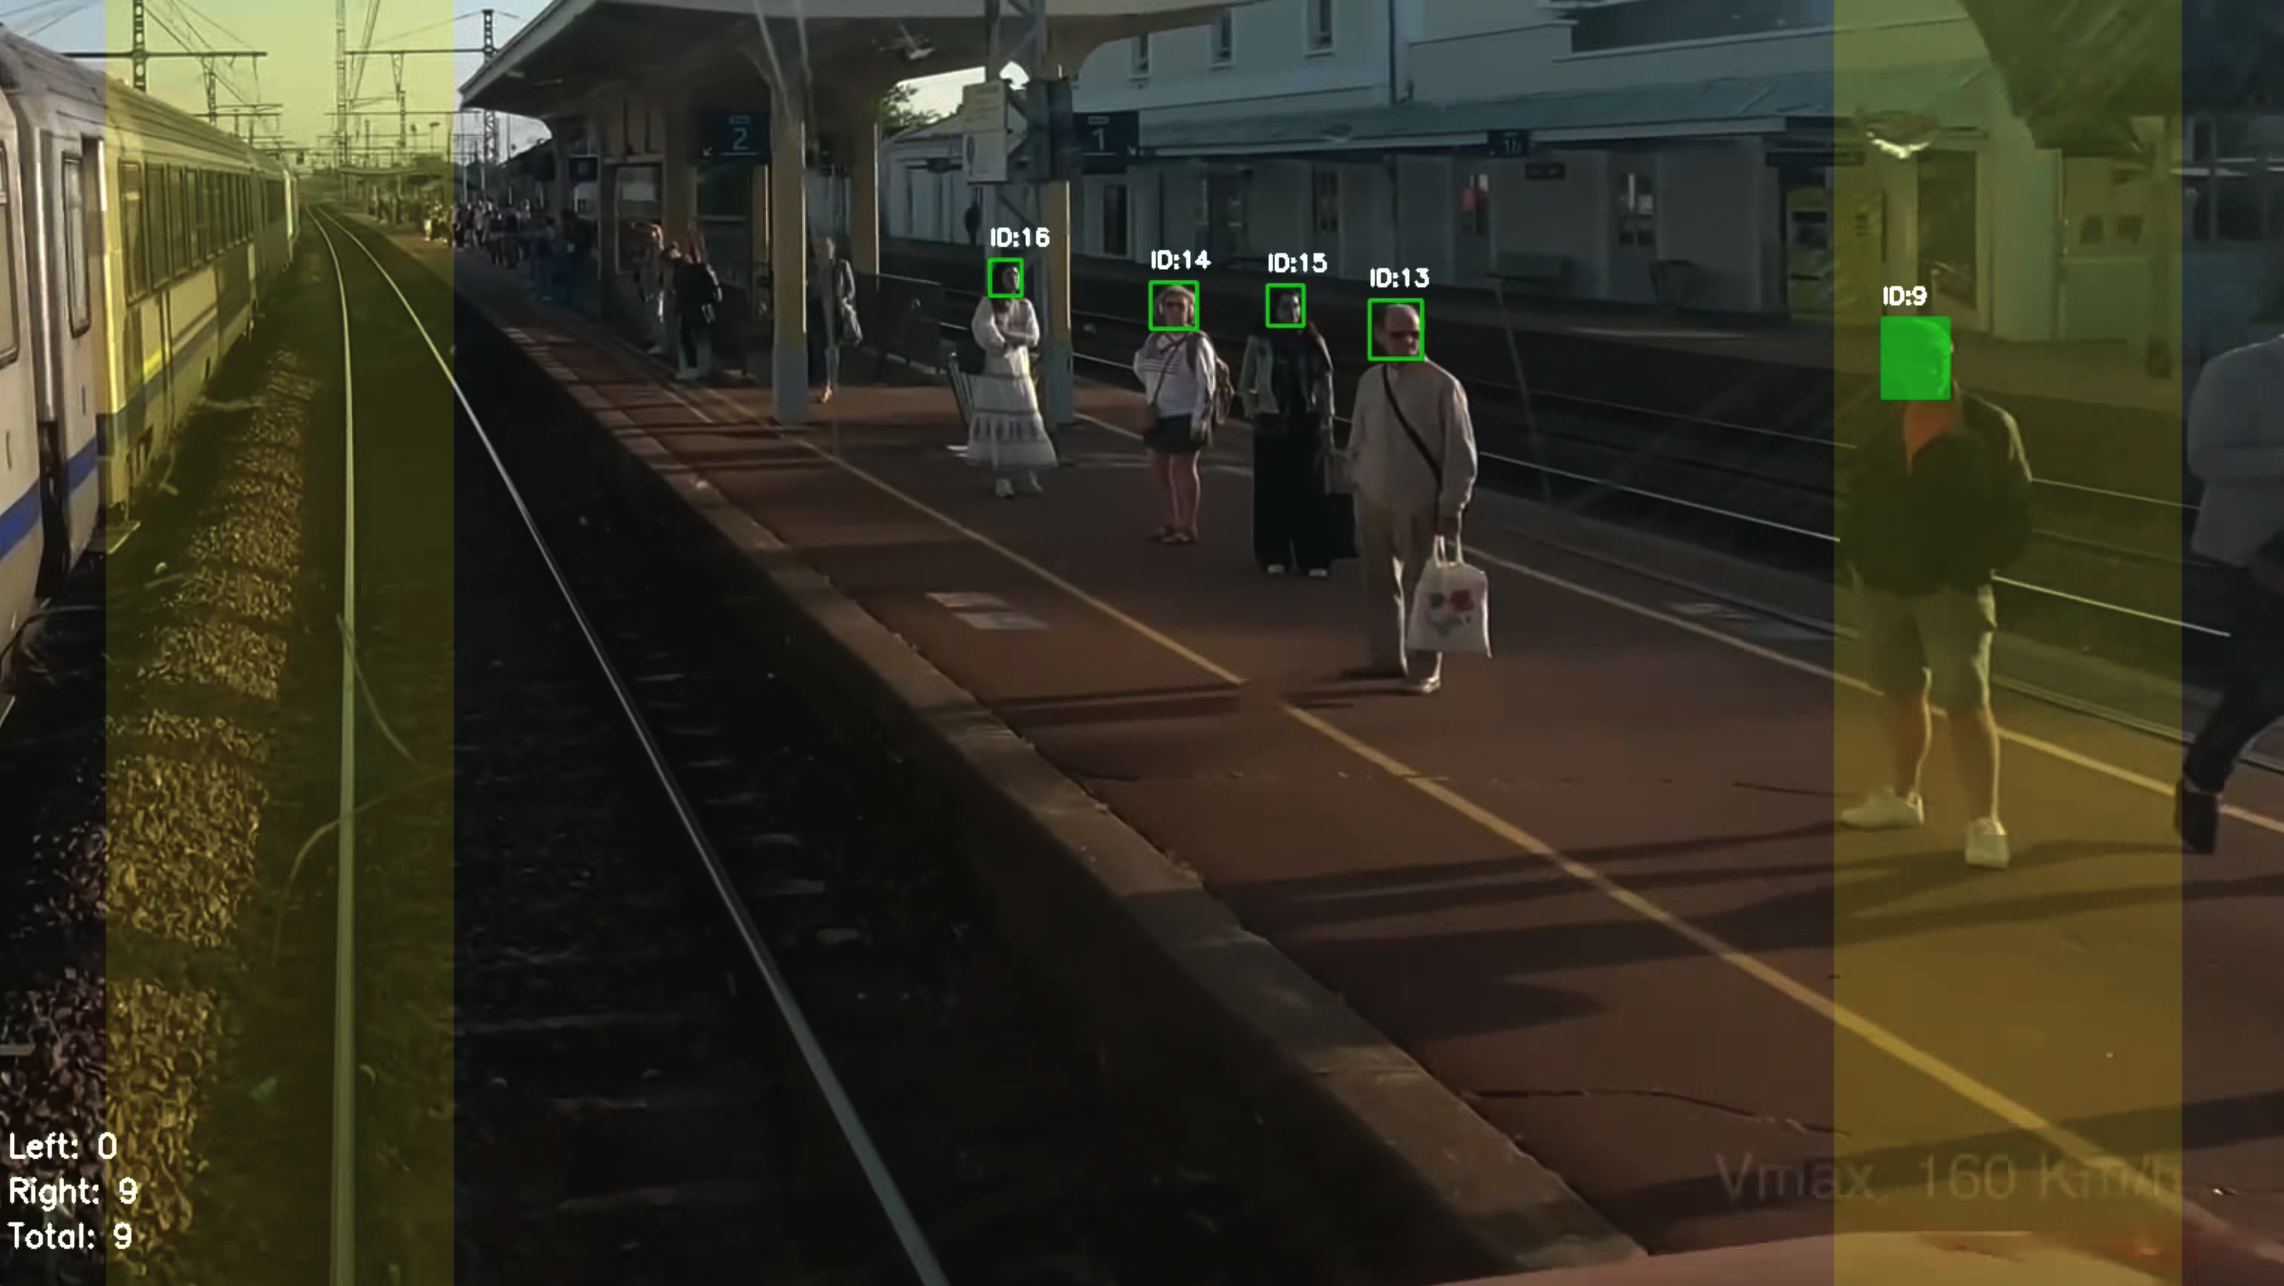
\includegraphics[width=0.8\textwidth]{pictures/P21CV8DResultsvideoFrame.png}
    \caption{8维状态向量模型追踪中间帧}
    \label{fig:P21CV8DResultsvideoFrame}
\end{figure}
% ---------------------------------------% 12维加速度模型（CA-12D）------------------------------------------------------------
3.2 12维加速度模型（CA-12D）
为解决基准模型（CV-8D）无法有效描述非线性运动的局限，我们引入了12维恒定加速度模型（Constant Acceleration， CA-12D）。该模型通过在状态向量中显式地增加加速度分量\ddot{x}, \ddot{y}, \ddot{a}, \ddot{h}， 旨在更精确地捕捉行人在站台场景中常见的变速行为，例如启动、停止、避让或因人群拥挤导致的短时速度.CA-12D的核心优势在于其更高阶的运动假设。如状态转移矩阵F所示，它采用了二阶泰勒展开来预测下一时刻的位置，理论上能更好地拟合非线性轨迹。这对于跟踪任务至关重要，尤其是在目标被短暂遮挡后，一个更准确的运动预测能够显著提高数据关联的成功率。

\paragraph{12维加速度模型（CA-12D）。} 在基准模型上扩展加速度分量，状态为 \([x, y, a, h, v_x, v_y, v_a, v_h, a_x, a_y, a_a, a_h]^\top\)，测量仍为 \([x, y, a, h]^\top\)。相较 CV-8D模型，能更好刻画进站减速、短时加减速与遮挡恢复阶段的状态变化。

\textbf{状态向量为：}
\begin{equation}
\mathbf{x}_k = [x, y, a, h, \dot{x}, \dot{y}, \dot{a}, \dot{h}, \ddot{x}, \ddot{y}, \ddot{a}, \ddot{h}]^T \in \mathbb{R}^{12}
\end{equation}

\textbf{状态转移矩阵为：}
\begin{equation}
\mathbf{F} = \begin{bmatrix}
\mathbf{I}_4 & \Delta t \cdot \mathbf{I}_4 & \frac{1}{2}\Delta t^2 \cdot \mathbf{I}_4 \\
\mathbf{0}_{4 \times 4} & \mathbf{I}_4 & \Delta t \cdot \mathbf{I}_4 \\
\mathbf{0}_{4 \times 4} & \mathbf{0}_{4 \times 4} & \mathbf{I}_4
\end{bmatrix}_{12 \times 12}
\end{equation}

\textbf{运动方程为：}
\begin{align}
\mathbf{p}_{k+1} &= \mathbf{p}_k + \mathbf{v}_k \Delta t + \frac{1}{2}\mathbf{a}_k \Delta t^2 \\
\mathbf{v}_{k+1} &= \alpha_v \mathbf{v}_{k+1}^{pred} + (1-\alpha_v) \mathbf{v}_k, \quad \alpha_v = 0.85 \\
\mathbf{a}_{k+1} &= \alpha_a \mathbf{a}_{k+1}^{pred} + (1-\alpha_a) \mathbf{a}_k, \quad \alpha_a = 0.7
\end{align}

\textbf{过程噪声协方差矩阵为：}
\begin{equation}
\mathbf{Q}_k = \text{diag}(\sigma_{pos}^2 h, \sigma_{vel}^2 h, \sigma_{acc}^2 h) \otimes \mathbf{I}_4
\end{equation}
其中 $\sigma_{pos} = 1/20$，$\sigma_{vel} = 1/160$，$\sigma_{acc} = 1/10$。

\textbf{观测向量为：}
\begin{equation}
\mathbf{z}_k = [x, y, a, h]^T \in \mathbb{R}^{4}
\end{equation}

\textbf{观测矩阵为：}
\begin{equation}
\mathbf{H} = [\mathbf{I}_4, \mathbf{0}_{4 \times 4}, \mathbf{0}_{4 \times 4}]_{4 \times 12}
\end{equation}
如\ref{tab:CV8DResults}所示，我们使用CA-12D模型，在MOT-TPCH数据集上达到了平均的67.54\%的MOTA，17.42\%的MOTP，75.29\%的IDF1，81.41\%的IDP，70.4\%的IDR，ID Switches为39，False Positive为278，precision为89.73\%，recall为77.51\%。其中，计数的相对平均误差6.99\%.
CA-12D模型相较于基准模型CV-8D，在多个方面展现了其优越性：
(1)首先，整体跟踪精度的提升：平均 MOTA 从 64.11\% 提升至 67.54\%。这一提升主要得益于误报（False Positives）的大幅减少（平均每视频从480个降至278个）。这有力地证明了加速度项的引入使得预测更为精准，当目标重现时，模型能更有效地将其与现有轨迹关联，而不是错误地创建一个新的虚假轨迹。

(2)其次，下游任务性能的显著改善：最关键的指标——计数相对平均误差——从14.59\%锐减至6.99\%，误差率降低了超过一半。这直接表明，尽管MOT指标的提升幅度有限，但更高阶的运动模型所带来的预测稳定性，对于计数这类需要长期身份保持的应用是至关重要的。如图 \ref{fig:CA12framedeomo} 所示，稳定的跟踪使得计数带能够准确地记录穿越事件。

(3)最后，模型的权衡与局限：然而，CA-12D也暴露了新的问题。其平均身份切换次数（ID Switches）从24次增加到39次。这揭示了一个潜在的陷阱：一个更复杂、更高维度的状态空间虽然拟合能力更强，但也可能对测量噪声更敏感，导致状态估计出现波动，从而在关联模糊时更容易发生身份错误。同时，其 IDF1 分数（75.29\%） 相较于基准模型（76.66\%）略有下降，也反映了在身份保持的纯粹性上存在一定牺牲。

综上所述，CA-12D模型通过引入加速度项，成功地提升了轨迹预测的准确性，显著降低了误报和最终的计数误差，证明了高阶运动模型在处理复杂动态场景时的价值。但其代价是身份稳定性的略微下降，显示了模型复杂性与鲁棒性之间的权衡。

\begin{table}[H]
    \centering
    \begin{tabular}{ccccccccccccccccccccc}
    \hline
        \textbf{Video} & \textbf{MOTA} & \textbf{MOTP} & \textbf{IDF1} & \textbf{IDP} & \textbf{IDR} & \textbf{ID Switches} & \textbf{Matches} & \textbf{False Positives} & \textbf{Misses} & \textbf{FAF} & \textbf{Precision} & \textbf{Recall} & \textbf{Mostly Tracked} & \textbf{Partially Tracked} & \textbf{Mostly Lost} & \textbf{Left Counting} & \textbf{Right Counting} & \textbf{Total Counting} & \textbf{Actual Counting} & \textbf{Relative Counting Error Rate } \\ \hline
        1 & 65.12 & 18.99 & 77.59 & 87.38 & 69.77 & 1 & 93 & 9 & 35 & 0.0909 & 91.26 & 72.87 & 2 & 2 & 0 & 0 & 4 & 4 & 4 & 0  \\ 
        2 & 56.46 & 17.08 & 74.25 & 86.01 & 65.31 & 2 & 373 & 54 & 190 & 0.2379 & 87.41 & 66.37 & 3 & 5 & 0 & 8 & 0 & 8 & 8 & 0  \\ 
        3 & 56 & 17.83 & 70.73 & 74.96 & 66.96 & 13 & 981 & 220 & 365 & 0.5288 & 81.88 & 73.14 & 12 & 10 & 3 & 26 & 1 & 26 & 25 & 4  \\ 
        4 & 75.49 & 16.82 & 79.94 & 78.61 & 81.32 & 11 & 593 & 88 & 65 & 0.3014 & 87.28 & 90.28 & 9 & 1 & 0 & 1 & 12 & 12 & 10 & 20  \\ 
        5 & 63.5 & 16.55 & 78.05 & 80.37 & 75.85 & 9 & 852 & 163 & 224 & 0.3396 & 84.08 & 79.35 & 12 & 5 & 1 & 19 & 0 & 19 & 18 & 5.56  \\ 
        6 & 80.63 & 16.37 & 79.01 & 80.91 & 77.2 & 19 & 2426 & 195 & 322 & 0.2932 & 92.61 & 88.36 & 12 & 4 & 0 & 17 & 0 & 17 & 16 & 6.25  \\ 
        7 & 52.47 & 19.55 & 57.61 & 71.05 & 48.44 & 27 & 1050 & 125 & 686 & 0.2399 & 89.6 & 61.09 & 6 & 10 & 5 & 0 & 22 & 22 & 21 & 4.76  \\ 
        8 & 58.83 & 17.26 & 73.44 & 80.06 & 67.83 & 36 & 2548 & 445 & 991 & 0.4159 & 85.31 & 72.28 & 22 & 21 & 4 & 1 & 45 & 45 & 47 & 4.26  \\ 
        9 & 73.29 & 16 & 79.16 & 87.97 & 71.96 & 140 & 10884 & 531 & 3102 & 0.262 & 95.4 & 78.04 & 72 & 50 & 2 & 0 & 123 & 123 & 124 & 0.81  \\ 
        10 & 81.04 & 17.8 & 87.05 & 90.3 & 84.03 & 5 & 1540 & 104 & 227 & 0.16 & 93.69 & 87.19 & 14 & 5 & 0 & 19 & 0 & 19 & 19 & 0  \\ 
        11 & 72.5 & 19.12 & 78.98 & 83.18 & 75.18 & 29 & 2541 & 266 & 568 & 0.3296 & 90.62 & 81.9 & 17 & 9 & 1 & 30 & 1 & 30 & 27 & 11.11  \\ 
        12 & 68.84 & 19.61 & 72.41 & 79.85 & 66.24 & 121 & 8369 & 724 & 2616 & 0.3102 & 92.14 & 76.45 & 36 & 28 & 0 & 80 & 0 & 80 & 64 & 25  \\ 
        13 & 77.72 & 16.06 & 83.36 & 91.89 & 76.28 & 5 & 499 & 14 & 120 & 0.0601 & 97.3 & 80.77 & 8 & 4 & 0 & 12 & 1 & 12 & 12 & 0  \\ 
        14 & 55.76 & 17.29 & 64.13 & 73.2 & 57.06 & 207 & 8023 & 1245 & 3925 & 0.6563 & 86.86 & 67.71 & 34 & 56 & 9 & 1 & 111 & 111 & 100 & 11  \\ 
        15 & 61.41 & 17.39 & 69.58 & 75.42 & 64.58 & 34 & 1932 & 304 & 685 & 0.438 & 86.61 & 74.16 & 14 & 12 & 2 & 28 & 0 & 28 & 28 & 0  \\ 
        16 & 60.94 & 17.2 & 70.89 & 72.31 & 69.53 & 40 & 2777 & 607 & 744 & 0.4814 & 82.27 & 79.11 & 20 & 12 & 0 & 1 & 35 & 35 & 32 & 9.38  \\ 
        17 & 73.97 & 15.5 & 83.79 & 85.2 & 82.44 & 9 & 1235 & 161 & 208 & 0.3418 & 88.54 & 85.67 & 12 & 3 & 1 & 0 & 15 & 15 & 16 & 6.25  \\ 
        18 & 77.81 & 15.88 & 69.34 & 72.36 & 66.56 & 16 & 1094 & 84 & 188 & 0.1244 & 92.96 & 85.52 & 3 & 3 & 0 & 7 & 0 & 7 & 6 & 16.67  \\ 
        19 & 78.3 & 17.53 & 86 & 90.31 & 82.08 & 7 & 1092 & 78 & 196 & 0.2746 & 93.37 & 84.86 & 15 & 7 & 2 & 0 & 21 & 21 & 24 & 12.5  \\ 
        20 & 60.8 & 18.48 & 70.59 & 86.93 & 59.42 & 52 & 2829 & 141 & 1540 & 0.1497 & 95.33 & 65.17 & 12 & 31 & 3 & 47 & 0 & 47 & 46 & 2.17  \\ 
        Average Value & 67.54 & 17.42 & 75.29 & 81.41 & 70.4 & 39.15 & 2586.55 & 277.9 & 849.85 & 0.3 & 89.73 & 77.51 & 16.75 & 13.9 & 1.65 & 14.85 & 19.55 & 34.05 & 32.35 & 6.99 \\ \hline
    \end{tabular}
    \caption{CA 12-Dimensional State Vector Model MOT and Count Evaluation Results}
    \label{tab:CA12DResults}
\end{table}

如\ref{fig:CA12framedeomo}所示，是CA-12D模型的评估视频过程中的某一帧，其中展示了当前帧的计数带，以及左计数带累计计数0人，右计数带累计计数10人，以及当前的总的计数结果10人，以及目标被跟踪的各个ID的情况。
\begin{figure}[H]
    \centering
    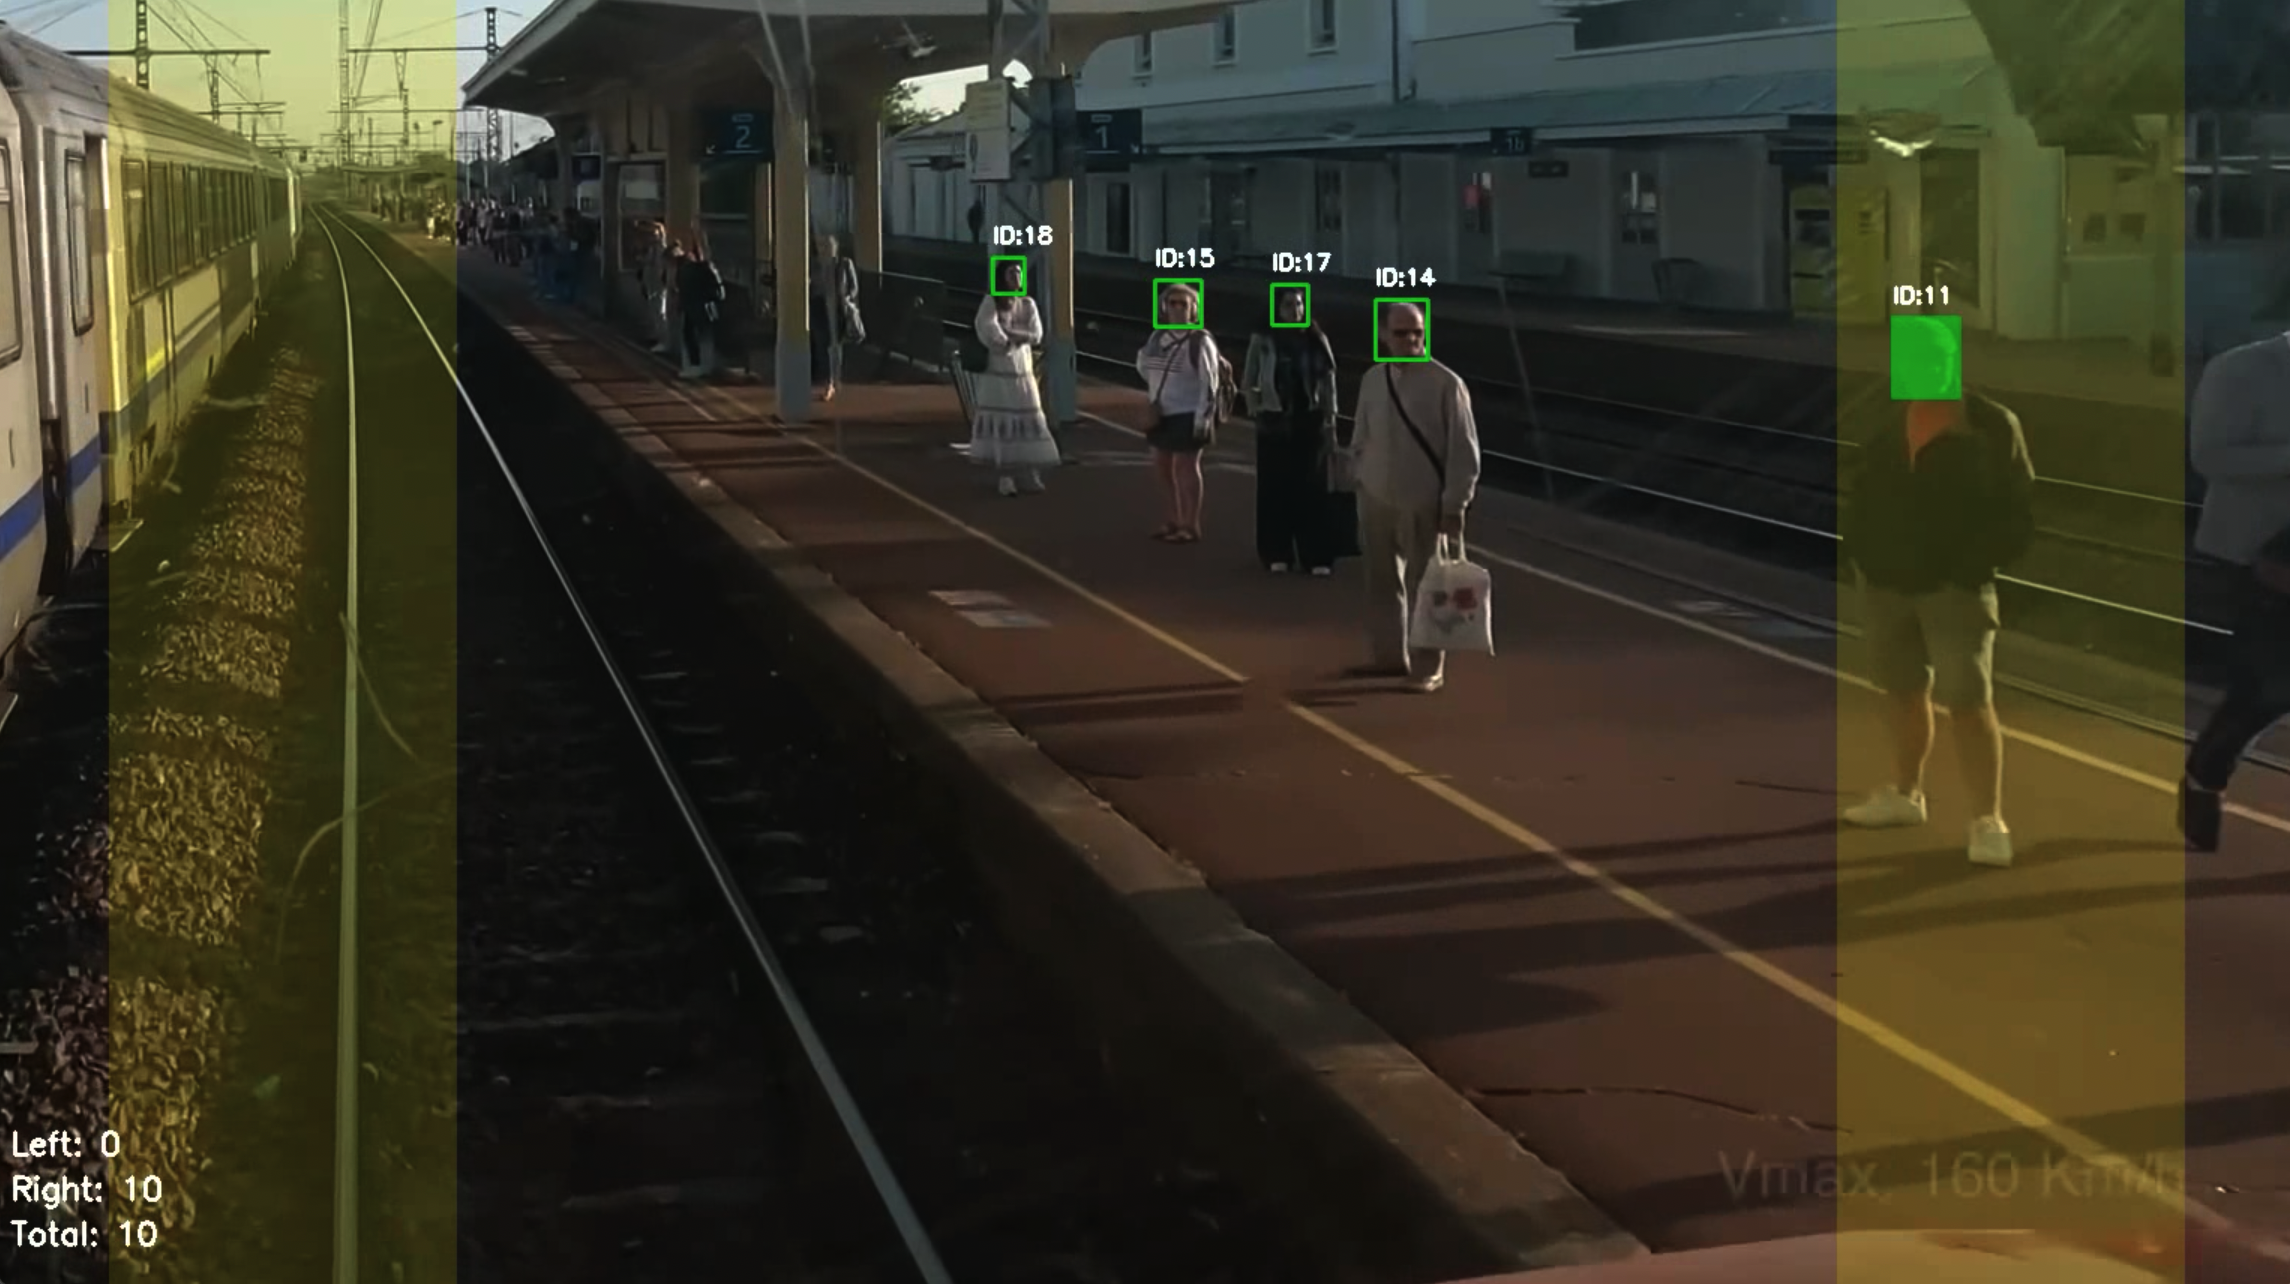
\includegraphics[width=0.8\textwidth]{pictures/CA12framedeomo.png}
    \caption{12维状态向量模型追踪中间帧展示}
    \label{fig:CA12framedeomo}
\end{figure}

% ---------------------------------------% 5维物理模型（Phys-5D）------------------------------------------------------------
3.3 5维物理模型（Phys-5D）
为克服纯粹基于图像平面运动学的局限性，我们提出了一个融合相机几何约束的5维物理模型 （Phys-5D）。该模型的核心创新在于将2D图像观测提升至3D物理空间进行状态估计，引入了场景的先验知识，旨在从根本上提高跟踪的稳定性和物理真实性。
Phys-5D模型不再将边界框的高度 \([H]\)视为一个独立的运动变量，而是通过针孔相机模型将其与目标的物理深度\([Z]\)进行强关联。状态向量直接对深度 \([Z]\) 及其变化率 Z进行估计。这种做法的优势在于：
首先，能保持物理一致性，目标的尺寸变化不再是任意的，而是严格受到其在3D空间中远离或靠近相机这一物理过程的约束。
其次，具备运动先验性，我们为深度方向的运动引入了自适应减速度约束。该约束模拟了行人在接近相机（或列车）时通常会减速的物理先验，有效抑制了因检测框抖动而导致的深度（即高度 h）剧烈变化的伪影。
最后，对状态空间进行了降维，尽管模型更复杂，但状态向量仅有5维，相比CA-12D更为紧凑，可能带来更好的估计效率和稳定性。
\paragraph{5维物理模型（Phys-5D）。} 融合针孔相机几何约束，将像素高度 \(h\) 与深度 \(Z\) 关联：\(Z = fH/h\)。状态取 \([u, v, h, Z, \dot Z]^\top\)，测量为 \([u, v, h]^\top\)。通过 \((X,Y,Z) \leftrightarrow (u,v,h)\) 的投影/反投影在预测时显式更新 \(Z\) 与 \(h\)，并对 \(\dot Z\) 引入减速度约束以贴合列车相对运动的物理先验。实现参考 \texttt{physical3dkf\_5d.py} 与 \texttt{deep\_sort/custom\_kf5d.py}。

\textbf{状态向量为：}
\begin{equation}
\mathbf{x}_k = [u, v, h_{px}, Z, \dot{Z}]^T \in \mathbb{R}^{5}
\end{equation}

\textbf{几何约束关系：}
\begin{equation}
h_{px} = \frac{f \cdot H}{Z}, \quad Z = \frac{f \cdot H}{h_{px}}
\end{equation}
其中 $f$ 为相机焦距（像素），$H = 0.3m$ 为行人头高。

\textbf{深度动力学模型：}
\begin{align}
Z_{k+1} &= Z_k + \dot{Z}_k \Delta t + \frac{1}{2}a_Z \Delta t^2 \\
\dot{Z}_{k+1} &= \dot{Z}_k + a_Z \Delta t
\end{align}

\textbf{自适应减速度约束：}
\begin{equation}
a_Z = -\text{sign}(\dot{Z}) \cdot \min\left(a_{max}, \frac{\dot{Z}^2}{2Z}\right), \quad a_{max} = 1.0 \text{m/s}^2
\end{equation}


\textbf{过程噪声协方差矩阵为：}
\begin{equation}
\mathbf{Q}_k = \text{diag}(\sigma_{pos}^2 h_{px}, \sigma_{pos}^2 h_{px}, \sigma_{pos}^2 h_{px}, \sigma_{vel}^2 h_{px}, \sigma_{vel}^2 h_{px})
\end{equation}
其中 $\sigma_{pos} = 1/2$，$\sigma_{vel} = 1/15$。

\textbf{观测向量为：}
\begin{equation}
\mathbf{z}_k = [u, v, h_{px}]^T \in \mathbb{R}^{3}
\end{equation}

\textbf{观测矩阵为：}
\begin{equation}
\mathbf{H} = \begin{bmatrix}
1 & 0 & 0 & 0 & 0 \\
0 & 1 & 0 & 0 & 0 \\
0 & 0 & 1 & 0 & 0
\end{bmatrix}_{3 \times 5}
\end{equation}
We note that despite physics constraints, the model remains image-based and is influenced by image quality and calibration uncertainties. We use fSpy to estimate intrinsics on a representative frame: 2K right: $f=795.0$, $(c_x,c_y)=(268.0,137.0)$; 2K left: $f=795.0$, $(1268.0,137.0)$; 4K right: $f=1600.3$, $(515.0,153.0)$; 4K left: $f=1600.3$, $(1789.0,153.0)$.

On MOT-TPCH (20 videos), Phys-5D achieves average MOTA=67.21\%, MOTP=17.41\%, IDF1=76.29\%, IDP=82.23\%, IDR=71.51\%, ID Switches=24.8, FP=290, Precision=89.06\%, Recall=77.45\%, and counting MAPE=2.24\% (Table~\ref{tab:Phys5DResults}). Notably, identity switches regress to baseline levels (24.8 vs 24), far below CA-12D (39), while counting error reaches the best level. This demonstrates that physics priors regularize state evolution, avoiding identity confusion from 2D size fluctuations, and translating into superior counting.
\begin{table}[H]
    \centering
    \begin{tabular}{ccccccccccccccccccccc}
    \hline
        \textbf{video} & \textbf{MOTA} & \textbf{MOTP} & \textbf{IDF1} & \textbf{IDP} & \textbf{IDR} & \textbf{ID Switches} & \textbf{Matches} & \textbf{False Positives} & \textbf{Misses} & \textbf{FAF} & \textbf{Precision} & \textbf{Recall} & \textbf{Mostly Tracked} & \textbf{Partially Tracked} & \textbf{Mostly Lost} & \textbf{left Counting} & \textbf{right Counting} & \textbf{total Counting} & \textbf{actual Counting} & \textbf{Relative Counting Error Rate } \\ \hline
        1 & 54.26 & 19.63 & 72.96 & 81.73 & 65.89 & 2 & 86 & 16 & 41 & 0.16 & 84.62 & 68.22 & 1 & 3 & 0 & 0 & 4 & 4 & 4 & 0  \\ 
        2 & 57.35 & 17.64 & 75.65 & 87.65 & 66.55 & 3 & 375 & 51 & 187 & 0.22 & 88.11 & 66.9 & 3 & 5 & 0 & 8 & 0 & 8 & 8 & 0  \\ 
        3 & 57.25 & 17.66 & 73.19 & 77.53 & 69.32 & 7 & 993 & 215 & 359 & 0.52 & 82.3 & 73.58 & 12 & 10 & 3 & 24 & 0 & 25 & 25 & 0  \\ 
        4 & 78.33 & 16.74 & 83.16 & 81.49 & 84.9 & 1 & 610 & 86 & 58 & 0.29 & 87.66 & 91.33 & 9 & 1 & 0 & 0 & 10 & 10 & 10 & 0  \\ 
        5 & 64.42 & 16.5 & 78.33 & 79.56 & 77.14 & 3 & 874 & 175 & 208 & 0.36 & 83.37 & 80.83 & 13 & 4 & 1 & 19 & 0 & 19 & 18 & 5.56  \\ 
        6 & 81.1 & 16.11 & 82.98 & 84.91 & 81.13 & 8 & 2440 & 196 & 319 & 0.29 & 92.59 & 88.47 & 13 & 3 & 0 & 16 & 0 & 16 & 16 & 0  \\ 
        7 & 53.72 & 19.9 & 63.01 & 75.52 & 54.06 & 15 & 1097 & 150 & 651 & 0.29 & 88.11 & 63.07 & 6 & 10 & 5 & 0 & 21 & 21 & 21 & 0  \\ 
        8 & 57.31 & 16.91 & 74.24 & 81.18 & 68.39 & 17 & 2522 & 473 & 1036 & 0.44 & 84.3 & 71.02 & 20 & 23 & 4 & 1 & 44 & 44 & 47 & 6.38  \\ 
        9 & 73.84 & 15.94 & 79.76 & 88.47 & 72.6 & 87 & 10968 & 537 & 3071 & 0.26 & 95.37 & 78.26 & 71 & 51 & 2 & 0 & 123 & 123 & 124 & 0.81  \\ 
        10 & 78.67 & 18.02 & 85.86 & 88.98 & 82.96 & 12 & 1517 & 123 & 243 & 0.19 & 92.55 & 86.29 & 14 & 5 & 0 & 19 & 0 & 19 & 19 & 0  \\ 
        11 & 71.41 & 19.41 & 76.45 & 80.95 & 72.43 & 35 & 2507 & 266 & 596 & 0.33 & 90.53 & 81.01 & 18 & 8 & 1 & 27 & 0 & 27 & 27 & 0  \\ 
        12 & 68.76 & 19.79 & 72.11 & 79.28 & 66.13 & 94 & 8403 & 766 & 2609 & 0.33 & 91.73 & 76.51 & 36 & 27 & 1 & 66 & 0 & 66 & 64 & 3.12  \\ 
        13 & 76.76 & 15.26 & 83.84 & 92.13 & 76.92 & 4 & 498 & 19 & 122 & 0.08 & 96.35 & 80.45 & 8 & 4 & 0 & 11 & 0 & 12 & 12 & 0  \\ 
        14 & 56.74 & 17.15 & 66.1 & 74.66 & 59.31 & 119 & 8217 & 1320 & 3819 & 0.7 & 86.33 & 68.58 & 34 & 58 & 7 & 0 & 100 & 100 & 100 & 0  \\ 
        15 & 62.28 & 17.2 & 71.93 & 78.18 & 66.62 & 16 & 1947 & 296 & 688 & 0.43 & 86.9 & 74.05 & 16 & 10 & 2 & 29 & 0 & 29 & 28 & 3.57  \\ 
        16 & 63.13 & 17.31 & 74.31 & 75.3 & 73.35 & 17 & 2850 & 602 & 694 & 0.48 & 82.65 & 80.51 & 21 & 11 & 0 & 0 & 31 & 32 & 32 & 0  \\ 
        17 & 72.73 & 15.43 & 82.94 & 84.76 & 81.2 & 11 & 1218 & 162 & 223 & 0.34 & 88.35 & 84.64 & 11 & 4 & 1 & 0 & 15 & 15 & 16 & 6.25  \\ 
        18 & 79.97 & 15.45 & 70.53 & 73.22 & 68.03 & 6 & 1119 & 81 & 173 & 0.12 & 93.28 & 86.67 & 3 & 3 & 0 & 6 & 0 & 6 & 6 & 0  \\ 
        19 & 75.37 & 17.63 & 84.94 & 89.28 & 81 & 5 & 1073 & 97 & 217 & 0.34 & 91.74 & 83.24 & 15 & 7 & 2 & 0 & 21 & 21 & 24 & 12.5  \\ 
        20 & 60.73 & 18.45 & 73.56 & 89.79 & 62.29 & 34 & 2859 & 174 & 1528 & 0.18 & 94.33 & 65.44 & 12 & 32 & 2 & 43 & 0 & 43 & 46 & 6.52  \\ 
        Average Value & 67.21  & 17.41  & 76.29  & 82.23  & 71.51  & 24.80  & 2608.65  & 290.25  & 842.10  & 0.32  & 89.06  & 77.45  & 16.80  & 13.95  & 1.55  & 13.45  & 18.45  & 32.00  & 32.35  & 2.24  \\ \hline
    \end{tabular}
    \caption{Phys-5-Dimensional state vector model mot and its count evaluation results}
    \label{tab:Phys5DResults}
\end{table}

如所示，是Phys-5D模型的评估视频过程中的某一帧，其中展示了当前统计的左右各计数带的人数，以及当前的计数结果，以及目标被跟踪的情况。
\begin{figure}[H]
    \centering
    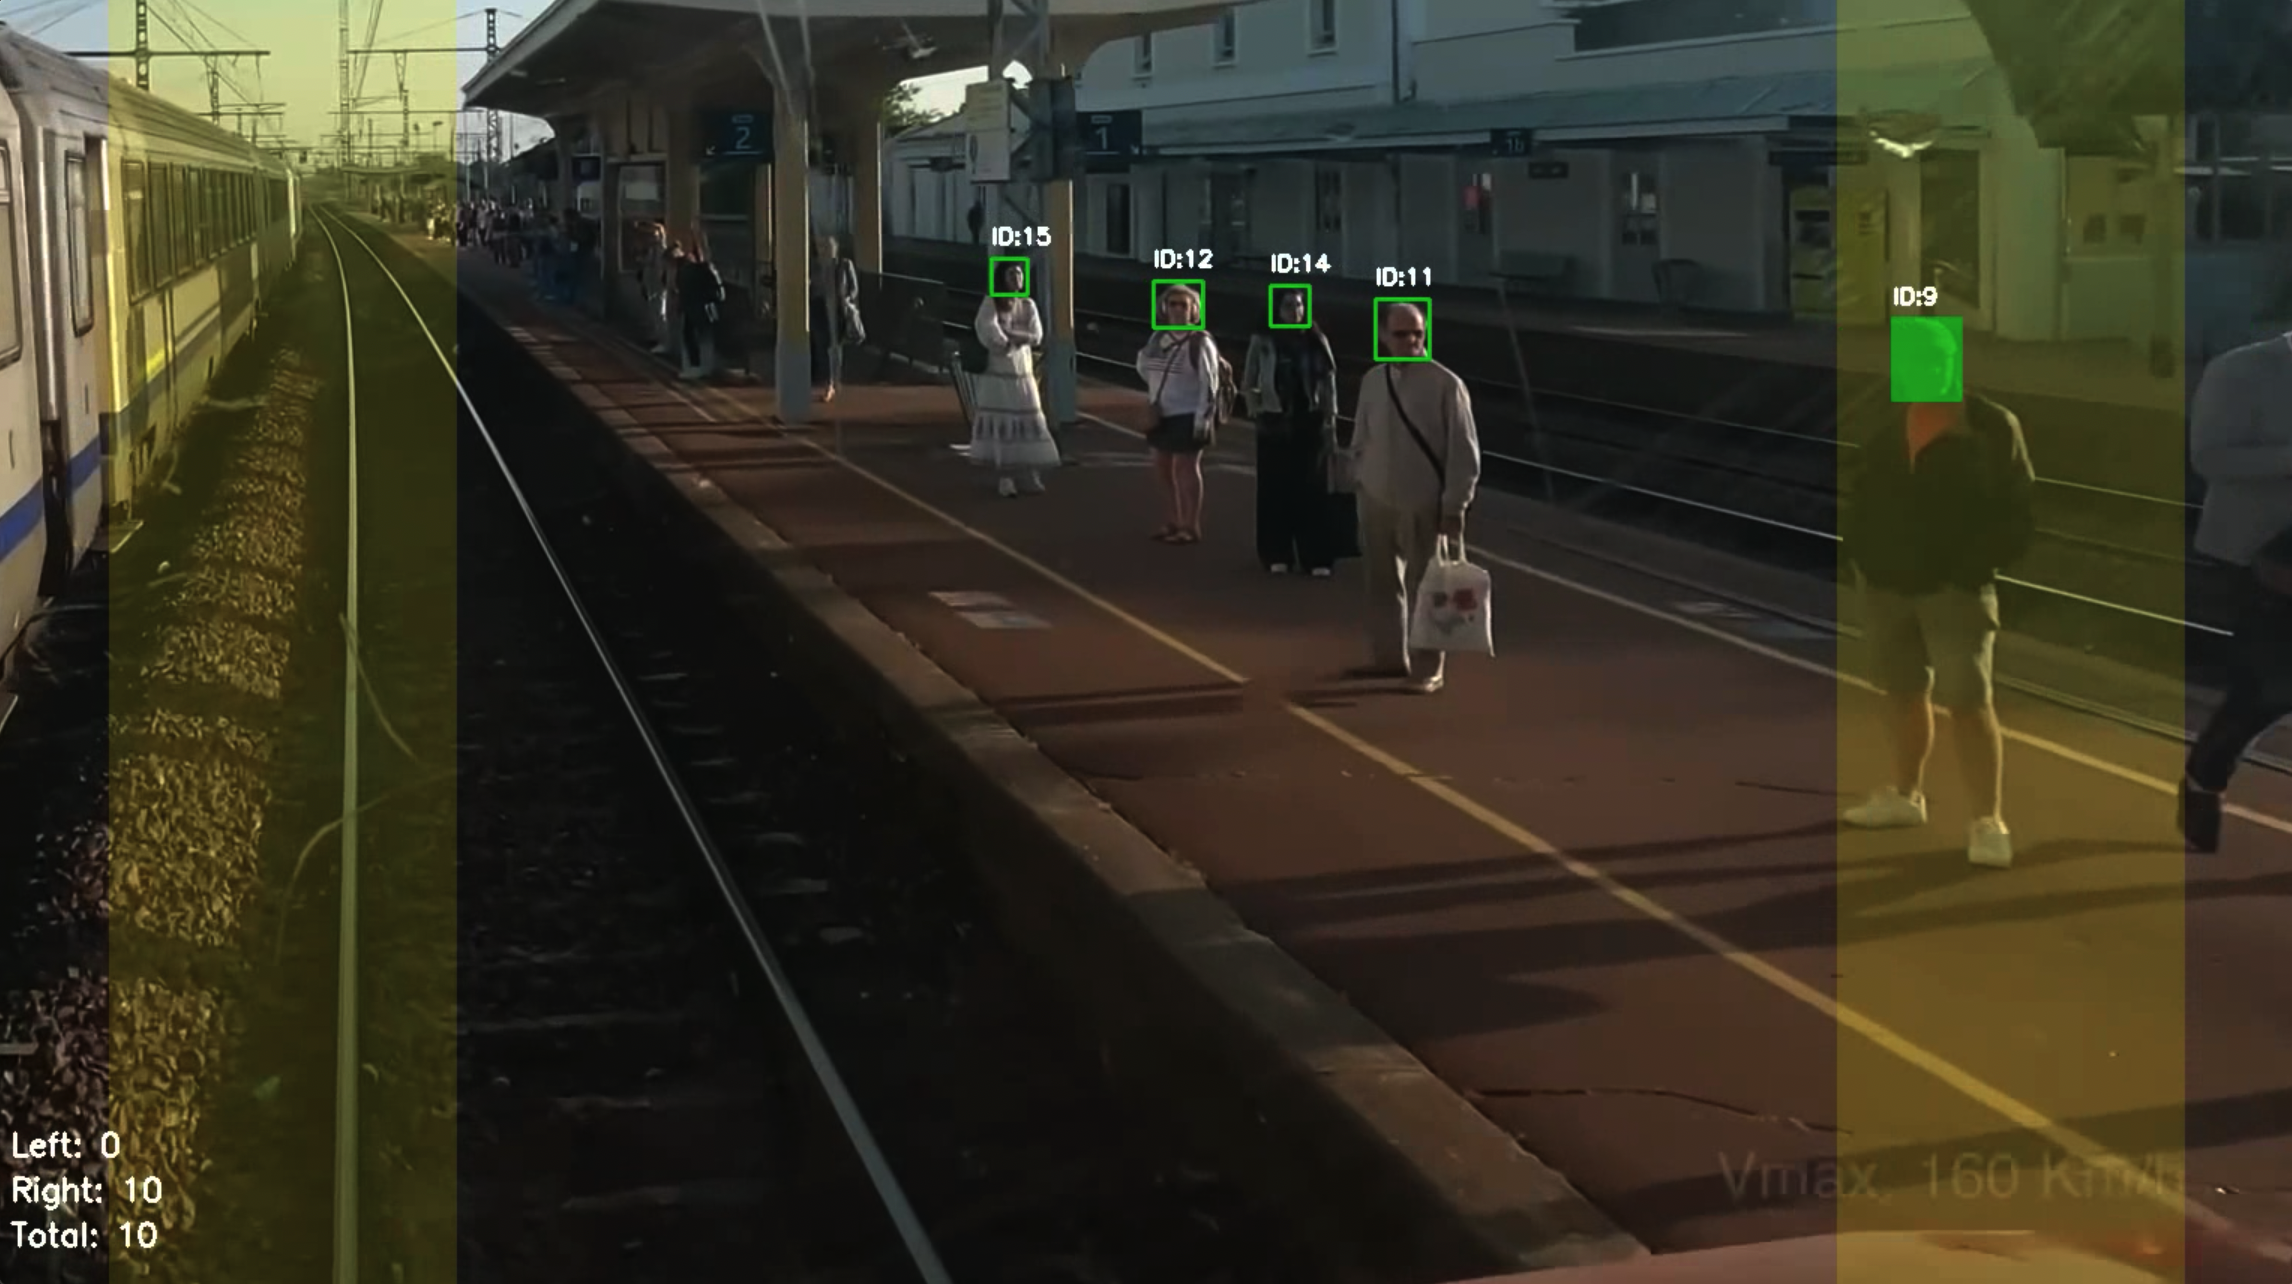
\includegraphics[width=0.8\textwidth]{pictures/Phys5Dframedeomo.png}
    \caption{5维状态向量模型追踪中间帧展示}
    \label{fig:Phys5Dframedeomo}
\end{figure}
因此，Phys-5D模型通过引入相机几何约束和物理运动先验，成功地将跟踪问题从2D图像域提升至3D物理域。这种方法极大地增强了轨迹预测的稳定性和合理性，尤其是在保持身份一致性方面表现突出，最终在关键的计数任务上取得了最佳性能。


3.4 三种不同复杂度运动模型的评估
最后，对三个模型的计数性能进行评估，按照第4章所提出的评估方法，我们得到了如\ref{tab:3modelsCountingComparisonResults}所示的结果，结果显示，在我们最关心的计数结果上，我们的Phys-5D模型得到了最好的结果。
\begin{table}[H]
    \centering
    \begin{tabular}{ccccc}
    \hline
        \textbf{Model} & \textbf{MAE } & \textbf{RMSE} & \textbf{MAPE(\%)} & \textbf{ME } \\ \hline
        \textbf{CV-8D} & 3.4 & 6.1514 & 14.592 & 1.4  \\ 
        \textbf{CA-12D} & 2.4 & 4.5837 & 6.99 & 0.7  \\ 
        \textbf{Phys-5D} & 0.75 & 1.3229 & 2.236 & -0.25 \\ \hline
    \end{tabular}
    \caption{Comparison of Counting Performance Across Three Motion Models}
    \label{tab:3modelsCountingComparisonResults}
\end{table}
通过对三种不同复杂度运动模型的系统性评估，我们得出以下结论：
（1）模型复杂度与性能并非简单的正相关。从CV-8D到CA-12D，增加运动学自由度（加速度）确实能提升对复杂动态的适应性，显著降低计数误差。但这种纯粹的运动学模型在更高维度下面临着身份保持能力下降的风险，显示了其内在的权衡。
（2）引入领域先验知识是提升跟踪鲁棒性的关键。Phys-5D模型虽然状态维度更低，但通过融合相机几何这一强物理先验，从根本上约束了状态估计的解空间。这不仅解决了CA-12D模型身份易切换的问题，更进一步将计数误差降至最低。
最终，我们的研究表明，专为特定场景设计的、融合了物理或几何先验的运动模型（如Phys-5D），相较于通用的纯运动学模型（无论是匀速还是加速度），能够在实现高精度跟踪的同时，提供更强的鲁棒性和身份一致性，尤其是在对长期稳定性要求苛刻的下游应用（如客流计数）中，其优势尤为突出。因此，Phys-5D是我们本次研究中提出的最优方案。

4.计数方法的消融实验
为系统性评估在第四章所提出的"虚拟计数带"计数方法的有效性，并探究其关键超参数的影响，本节设计了消融实验。该方法的核心是通过设置具有宽度的计数区域，并结合持续帧检测策略，以克服传统计数线因轨迹抖动或短暂遮挡所导致的漏计与误计问题。本实验将重点考察计数带的起始（Start）与终止（End）位置对最终计数精度的影响。

如\ref{fig:VirtualCountingZone}所示，展示了虚拟计数带的设置图，以Start=0.05，End=0.2为例。其中的start和End的数值表示该区域的起止线距离图像边界的距离占图像宽度的比例，start=0.05,end=0.2,表示了计数区域从0.05x图像宽度到0.2x图像宽度的区域，左右对称有两块区域，。当start=end的时候，表示使用的是计数线的计数方法。
\begin{figure}[H]
    \centering
    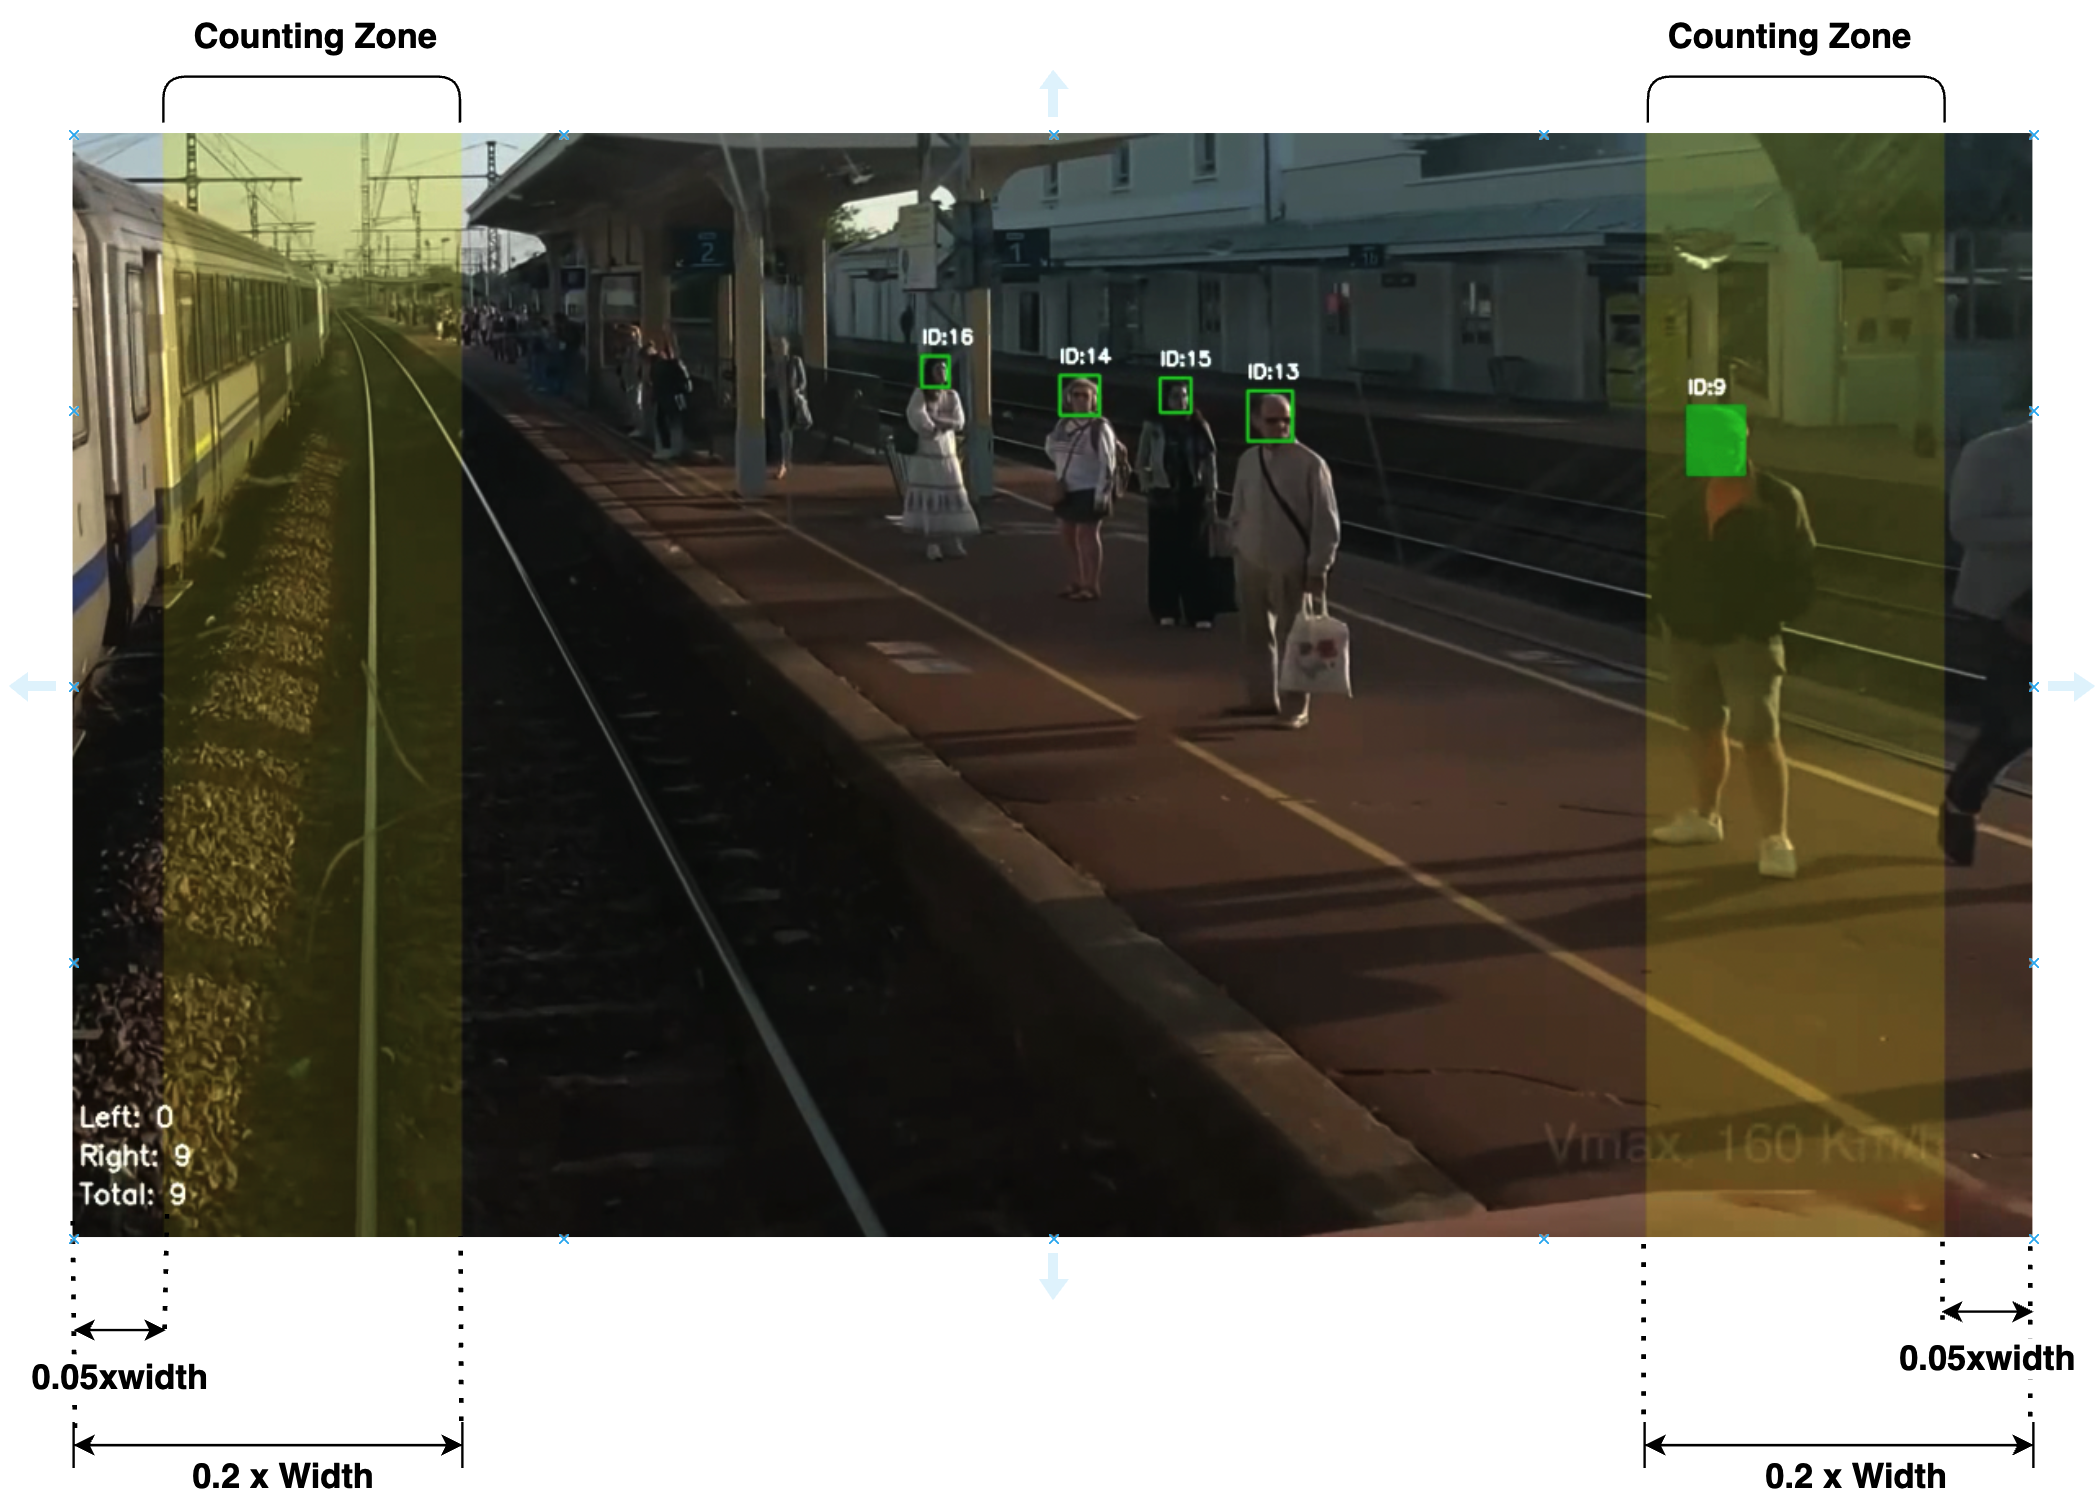
\includegraphics[width=0.8\textwidth]{pictures/VirtualCountingZone.png}
    \caption{Schematic Diagram of the Virtual Counting Zone}
    \label{fig:VirtualCountingZone}
\end{figure}

如表 \ref{tab:CountingbandAblationExperiment} 所示，我们进行了一项消融实验，旨在系统性地探究计数带的起始（Start）与终止（End）位置这两个关键超参数对模型计数性能的影响。实验结果清晰地揭示了模型的性能对计数带的宽度与位置具有高度敏感性，并证明了存在一个最优的配置区间。
\begin{table}[H]
    \centering
    \caption{Results of counting band and line ablation experiment}
    \begin{tabular}{cccccc}
    \hline
        \textbf{Start} & \textbf{End} & \textbf{MAE} & \textbf{RMSE} & \textbf{MAPE(\%)} & \textbf{ME } \\ \hline
        0.05  & 0.20  & 0.90  & 1.38  & 2.97  & -0.20   \\ 
        0.05  & 0.15  & 1.15  & 1.75  & 4.07  & -0.95   \\ 
        0.00  & 0.15  & 1.25  & 1.77  & 4.67  & -0.15   \\ 
        0.10  & 0.20  & 1.40  & 2.10  & 5.28  & -1.10   \\ 
        0.00  & 0.20  & 1.50  & 2.14  & 4.97  & 0.60   \\ 
        0.15  & 0.30  & 1.50  & 2.37  & 8.58  & 0.20   \\ 
        0.00  & 0.10  & 1.80  & 2.57  & 5.83  & -1.60   \\ 
        0.10  & 0.25  & 1.80  & 2.68  & 6.94  & 0.30   \\ 
        0.20  & 0.30  & 2.05  & 2.89  & 9.66  & -0.85   \\ 
        0.05  & 0.25  & 2.10  & 2.93  & 6.55  & 1.10   \\ 
        0.15  & 0.25  & 2.10  & 2.81  & 9.57  & -1.30   \\ 
        0.20  & 0.35  & 2.40  & 3.44  & 10.61  & 1.10   \\ 
        0.10  & 0.30  & 2.45  & 3.68  & 8.55  & 1.65   \\ 
        0.10  & 0.15  & 2.60  & 3.65  & 9.81  & -2.50   \\ 
        0.00  & 0.25  & 2.75  & 3.94  & 8.59  & 1.85   \\ 
        0.05  & 0.10  & 2.75  & 3.56  & 8.78  & -2.55   \\ 
        0.05  & 0.30  & 2.85  & 4.46  & 8.56  & 2.45   \\ 
        0.15  & 0.35  & 2.85  & 4.42  & 11.16  & 1.95   \\ 
        0.30  & 0.40  & 3.05  & 4.17  & 15.38  & -0.55   \\ 
        0.15  & 0.20  & 3.15  & 4.38  & 11.45  & -3.05   \\ 
        0.20  & 0.25  & 3.50  & 4.93  & 12.89  & -2.80   \\ 
        0.30  & 0.35  & 3.50  & 4.43  & 16.85  & -3.40   \\ 
        0.00  & 0.30  & 3.60  & 5.53  & 10.81  & 3.20   \\ 
        0.10  & 0.35  & 3.90  & 6.43  & 11.85  & 3.30   \\ 
        0.20  & 0.40  & 4.15  & 6.43  & 16.10  & 3.35   \\ 
        0.05  & 0.35  & 4.30  & 7.44  & 11.85  & 4.10   \\ 
        0.15  & 0.40  & 4.65  & 7.55  & 16.81  & 4.15   \\ 
        0.00  & 0.35  & 5.00  & 8.54  & 13.79  & 4.80   \\ 
        0.10  & 0.40  & 5.80  & 9.62  & 17.90  & 5.50   \\ 
        0.00  & 0.05  & 5.95  & 7.77  & 18.77  & -5.95   \\ 
        0.05  & 0.40  & 6.30  & 10.62  & 18.11  & 6.30   \\ 
        0.00  & 0.40  & 7.00  & 11.72  & 20.05  & 7.00   \\ 
        0.30  & 0.30  & 31.10  & 43.49  & 92.71  & -31.10   \\ 
        0.05  & 0.05  & 31.30  & 43.69  & 93.55  & -31.30   \\ 
        0.15  & 0.15  & 31.30  & 43.67  & 93.58  & -31.30   \\ 
        0.10  & 0.10  & 31.35  & 43.74  & 93.66  & -31.35   \\ 
        0.20  & 0.20  & 31.35  & 43.74  & 93.66  & -31.35  \\ \hline
    \end{tabular}
    \label{tab:CountingbandAblationExperiment}
\end{table}
1. 最优配置的性能表现：
在所有测试的组合中，当计数带设置为 `[0.05, 0.20]` 区间时，模型展现出最佳的计数性能。在该配置下，所有误差指标均达到最小值：平均绝对误差（MAE）为0.90，均方根误差（RMSE）为1.38，平均绝对百分比误差（MAPE）低至2.97\%。同时，其平均误差（ME）为-0.20，一个接近于零的数值，表明该配置下的计数结果几乎是无偏的，仅存在极轻微的漏计倾向。这一结果为后续实验和应用提供了最佳参数基准。

2. 计数带过窄（趋近于线）的性能退化：
一个极端情况是当起始与终止位置相同（`Start = End`）时，计数带退化为传统的计数线。表格末尾的数据（例如，`[0.30, 0.30]` 或 `[0.05, 0.05]`）显示，这种配置导致了性能的灾难性下降。MAE值从最优的0.90急剧恶化至约31.3，增大了超过30倍；MAPE也从2.97\%飙升至93\%以上。更重要的是，ME值呈现出巨大的负值（约-31.3），这提供了强有力的量化证据，证实了计数线方法存在极其严重的系统性漏计偏差。这与我们的假设相符，即单薄的计数线对目标轨迹的微小抖动或检测的瞬时中断（detection noise）缺乏鲁棒性，极易造成穿越事件的遗漏。

3. 计数带过宽的性能影响：
与此相对，当计数带设置得过宽时，尽管性能远优于计数线，但相较于最优配置仍有显著下滑。以 `[0.00, 0.40]` 这一较宽的区间为例，其MAE（7.00）和RMSE（11.72）分别是最佳配置的7倍和8倍以上。值得注意的是，该配置下的ME为+7.00，呈现出显著的正向偏差。这有力地支持了我们的观点：过宽的区域增加了目标在区域内停留的时间，从而增大了因身份（ID）切换或轨迹不稳定而导致同一目标被重复计数的风险，引发了显著的多计（overcounting）现象。

结论：
综上所述，本次消融研究清晰地证明了计数带的宽度选择是一个在"避免漏计"与"防止多计"之间的权衡（trade-off）。过窄的计数带（尤其是计数线）对噪声敏感，导致严重漏计；而过宽的计数带则会因ID切换等问题引入多计误差。实验数据表明，宽度适中的计数带，特别是 `[0.Sstart=0.05, End=0.20]` 的配置，能够在对轨迹扰动的鲁棒性与计数的唯一性、精确性之间达到最佳平衡，从而实现最优的计数性能。

如\ref{tab:ComparisonofAverage}所示，展示了计数线和计数带的平均指标，我们可以很明显地从表中得出，计数线的计数性能远不如计数带计数。
\begin{table}[H]
    \centering
    \caption{Comparison of Average Counting Metrics between Counting Lines and Counting Zones}
    \begin{tabular}{ccccc}
    \hline
        \textbf{} & \textbf{MAE} & \textbf{RMSE} & \textbf{MAPE(\%)} & \textbf{ME } \\ \hline
        Average metrics of line-crossing counting & 31.28  & 43.66  & 93.43  & -31.28   \\ 
        Average counting metrics of counting zones & 3.13  & 4.75  & 10.87  & 0.81  \\ \hline
    \end{tabular}
    \label{tab:ComparisonofAverage}
\end{table}
根据表 \ref{tab:ComparisonofAverage} 所呈现的计数线与计数带两种方法的平均性能指标对比，可以明确地观察到两者在计数精度上存在显著差异。这些数据为我们采用计数带方法提供了强有力的量化支持，具体分析如下：

首先，在误差幅度方面：计数线的平均绝对误差（MAE）高达31.28，而计数带的MAE仅为3.13。这表明，从绝对误差的平均水平来看，计数带方法的准确度比计数线方法高出一个数量级。同样，均方根误差（RMSE）指标也反映了同样的趋势，计数线（43.66）的RMSE远高于计数带（4.75）。RMSE对较大误差更为敏感，如此巨大的差距进一步说明计数线方法不仅平均误差大，而且更容易出现偏差较大的极端错误，系统的稳定性较差。

其次，在相对误差与偏差方面：平均绝对百分比误差（MAPE）的对比尤为突出。计数线的MAPE达到了惊人的93.43\%，这意味着其平均误差几乎与计数的真值相当，从相对意义上讲，这种方法的计数结果几乎不具备参考价值。相比之下，计数带的MAPE为10.87\%，这是一个在许多应用场景中都可以接受的误差水平。此外，从平均误差（ME）来看，计数线的ME为-31.28，揭示了该方法存在着严重的、系统性的漏计（undercounting）偏差。而计数带的ME为0.81，非常接近于0，表明其计数结果几乎是无偏的，仅有极轻微的高估倾向，这在统计学上意味着更高的可靠性。

综上所述，无论是从绝对误差、相对误差还是系统偏差的角度进行评估，计数带方法在各项关键性能指标上均全面优于计数线方法。其不仅计数结果的误差更小，而且表现出更高的稳定性和更低的偏差。因此，表 \ref{tab:ComparisonofAverage} 中的数据无可辩驳地证明了，为了获得高精度的计数结果，选择计数带是一种更为合理且有效的方法论。

\subsection{总结}
本章通过一系列系统的实验，全面验证了我们提出的"检测-跟踪-计数"框架的有效性。实验结果以详实的数据，层层递进地证明了各模块优化及最终方案的优越性。

\textbf{1. 高精度检测器的构建：} 实验始于检测器的优化。通过"通用预训练+领域微调"的两阶段策略，YOLOv11m检测器的性能得到巨大提升。在我们的目标场景数据集上，模型的\textbf{mAP50从79.4\%跃升至98.0\%}，而衡量定位精度的\textbf{mAP50–95也从54.7\%显著提高到81.6\%}。这一高精度的检测器为后续的跟踪与计数任务提供了坚实可靠的基础。

\textbf{2. 跟踪模型的量化对比：} 本章的核心在于对三种运动模型的深度评估。实验数据显示：
\begin{itemize}
    \item 基准模型 \textbf{CV-8D} 确立了性能基线，其计数平均绝对百分比误差（MAPE）高达 \textbf{14.59\%}。
    \item \textbf{CA-12D} 模型通过引入加速度项，将计数 MAPE 显著降低至 \textbf{6.99\%}，证明了高阶运动模型对复杂动态的更强拟合能力。但其代价是身份切换（ID Switches）次数从24次增加到39次，暴露了其在身份保持上的不稳定性。
    \item 我们提出的 \textbf{Phys-5D} 物理模型表现出最佳的综合性能。它不仅将平均身份切换次数控制在与基准相当的 \textbf{24.8} 次，维持了卓越的身份一致性，更是在关键的计数任务上取得了决定性优势，将 \textbf{MAPE 降至2.24\%}，平均绝对误差（MAE）仅为 \textbf{0.75}。
\end{itemize}

\textbf{3. 计数方法的有效性验证：} 计数方法的消融实验同样得出了明确结论。我们提出的虚拟计数带方法（最优配置下 MAE 为 0.90, MAPE 为 2.97\%）远优于传统的计数线方法。数据显示，计数线方法的 \textbf{MAE 高达 31.28}，\textbf{MAPE 超过 93\%}，并存在严重的系统性漏计问题（ME ≈ -31.3），证明了计数带设计对于保证计数鲁棒性的必要性。

综上所述，本章的实验结果有力地证明了，我们最终采用的"高精度YOLOv11m检测器 + Phys-5D物理跟踪模型 + 优化虚拟计数带"的技术路径，是解决特定站台场景下人群计数的优越方案。其中，Phys-5D模型通过融合物理先验知识，在跟踪精度、身份保持和计数准确性之间取得了最佳平衡，其 \textbf{2.24\%} 的计数误差充分验证了该方法的有效性和先进性。
\fi
\clearpage
\section{Discussion}\label{section::Discussion}


This chapter provides comprehensive analysis and interpretation of the experimental results presented in Chapter 5. We investigate the fundamental reasons behind performance differences among the three Kalman state-space configurations, elucidate why the proposed physics-constrained model (Phys-5D) achieves superior performance, and analyze the synergistic interactions between system components. We further discuss theoretical implications, practical value, and limitations, providing insights for future research directions.

\subsection{Comprehensive Interpretation of Results and Core Findings}

The experimental results from Chapter 5 demonstrate the effectiveness of our detect–track–count framework. Our final system achieves state-of-the-art counting accuracy with MAPE=2.24\%, representing a significant improvement over baseline approaches. The key findings from our comprehensive evaluation are:

\textbf{Performance Summary:} The three Kalman state-space configurations show distinct performance characteristics:
\begin{itemize}
    \item CV-8D (baseline): MAPE=14.59\%, MAE=3.4, ID switches=24
    \item CA-12D (acceleration): MAPE=6.99\%, MAE=2.4, ID switches=39.15
    \item Phys-5D (physics-constrained): MAPE=2.24\%, MAE=0.75, ID switches=24.8
\end{itemize}

\textbf{Core Finding:} The results demonstrate that incorporating domain knowledge (camera geometry and physical constraints) into the motion model is far more effective than merely increasing kinematic model complexity. Phys-5D achieves the best balance between tracking accuracy and identity consistency, translating to superior counting performance.

An important observation is that application performance (counting accuracy) is not linearly correlated with traditional MOT metrics (e.g., MOTA). CA-12D and Phys-5D obtain nearly identical MOTA (67.54\% vs 67.21\%), suggesting similar per-frame detection–association accuracy. However, this obscures a critical difference: the number of IDSW is much higher for CA-12D (avg 39.15) than for Phys-5D (avg 24.80). Identity switches measure how well a tracker preserves identity consistency. For cumulative tasks like counting, which require long-term, stable, and unique identities, trajectory stability and persistent identity are more important than single-frame localization accuracy. Each identity switch can cause the same person to be mistaken for two different identities, inducing overcounts or undercounts. Hence, although CA-12D can fit instantaneous motion better, its weaker identity consistency directly leads to much higher counting errors than Phys-5D. This highlights that application-oriented evaluations must emphasize identity-consistency metrics such as IDF1 and IDSW. Phys-5D’s true advantage lies not only in accurate tracking but also in sustaining consistent identities.

\subsection{Motion Models: From Pure Kinematics to Physics-Constrained Modeling and the Trade-offs}

To uncover the origins of performance differences among motion models, we now compare the three variants evaluated—CV-8D, CA-12D, and Phys-5D—and argue why imposing physics constraints is key to success in our task.

\subsubsection{Limitations of the Baseline (CV-8D)}

As the standard baseline in MOT, the CV-8D model is our starting point. It assumes linear, constant-speed motion in the image plane. In our scenario—platform pedestrians observed from a moving train—this assumption is fundamentally violated. As the train decelerates, perspective projection causes apparent nonlinear acceleration of pedestrians in the image plane and a nonlinear enlargement of their bounding boxes.
The experimental evidence confirms this mismatch. As shown in \textbf{Tab.}~\ref{tab:CV8DResults}, CV-8D exhibits many misses (avg 645) and a high counting error (MAPE 14.59\%). The root cause is that during occlusions, the constant-velocity Kalman filter cannot predict the object’s reappearance position and size accurately. Large deviations between prediction and observation (i.e., large Mahalanobis distance) lead to association failures: the tracker either terminates the original trajectory (misses) or allocates a new identity upon reappearance (ID switches). The performance bottleneck is thus that constant velocity assumptions cannot effectively predict accurate positions in the next frame.

\subsubsection{Gains and Losses of the Higher-Order Kinematic Model (CA-12D)}

A straightforward improvement to CV-8D is to raise the kinematic order by adding accelerations. The CA-12D model embodies this idea and can, in principle, fit nonlinear motion trajectories.
The data partially validate this: relative to CV-8D, CA-12D improves MOTA from 64.11\% to 67.54\% and reduces counting MAPE from 14.59\% to 6.99\%. This stems mainly from better prediction after short occlusions, which increases successful associations and substantially reduces false positives (avg from 480 to 278).
However, CA-12D introduces an unintended drawback: identity switches rise from 24 to 39.15, even exceeding those of the simpler CV-8D. This reveals a typical challenge in high-dimensional state estimation: while higher dimensionality increases expressiveness, it also amplifies sensitivity to measurement noise. YOLOv11 detections inevitably contain small frame-to-frame jitters. CA-12D may interpret such tiny jitters as large instantaneous accelerations, destabilizing state estimates. Unstable predictions disrupt association, particularly in crowded, ambiguous settings, and increase identity mis-assignments. The lesson is clear: without strong constraints, simply adding degrees of freedom may improve trajectory fitting but harm robustness to noise and, consequently, identity consistency.

\subsubsection{Why the Physics-Constrained Model (Phys-5D) Prevails}

Motivated by CA-12D’s trade-offs, we propose Phys-5D, which lifts estimation from the 2D image plane to the 3D physical domain and leverages inherent geometric constraints.
The key is to use the pinhole camera model to establish a deterministic, nonlinear relation between the 2D image height $h$ (px) and the 3D depth $Z$. This acts as a strong regularizer: height jitters are no longer arbitrary size changes but physically interpreted as small movements along depth. Advantages include: (1) physical realism by enforcing perspective consistency and suppressing artifacts; (2) incorporation of priors via an adaptive deceleration constraint that reflects real behavior as pedestrians approach the camera/train; and (3) reduced state dimensionality and improved stability—a compact 5D state with a highly constrained solution space enables robust inference from noisy observations, directly addressing CA-12D’s instability.
Empirically, Phys-5D achieves the best balance (\ref{tab:Phys5DResults}). Its MOTA (67.21\%) is comparable to CA-12D, but ID switches regress to baseline levels (24.80, on par with CV-8D). This stability translates to the application level: counting MAPE drops to 2.24\%.
To visualize the trade-offs and evolution across models, we summarize key metrics below.
As in Table \ref{tab:3modelsCountingComparisonResults}, a comparison of the three motion models:

\begin{table}[H]
    \centering
    \resizebox{0.6\textwidth}{!}{%
    \small
    \begin{tabular}{ccccc}
    \hline
        \textbf{Model} & \textbf{MAE } & \textbf{RMSE} & \textbf{MAPE(\%)} & \textbf{ME } \\ \hline
        \textbf{CV-8D} & 3.4 & 6.1514 & 14.592 & 1.4  \\ 
        \textbf{CA-12D} & 2.4 & 4.5837 & 6.99 & 0.7  \\ 
        \textbf{Phys-5D} & 0.75 & 1.3229 & 2.236 & -0.25 \\ \hline
    \end{tabular}%
    }
    \caption{Counting Performance Comparison of the Three Models}
    \label{tab:3modelsCountingComparisonResults}
\end{table}

The table makes the evolution clear: from CV-8D to CA-12D, we improved motion fitting at the expense of identity stability; from CA-12D to Phys-5D, imposing physics constraints not only restored and surpassed identity stability but also pushed application accuracy to a new level. Phys-5D is thus the optimal solution for our task.

\subsection{Synergy and Contributions of System Components}

Although the motion model is central, the system’s success results from carefully designed components working together. The detect–track–count pipeline is a chain whose overall strength depends on every link.
Detector as the foundation: the upper bound of tracking is largely determined by detector quality. Our two-stage strategy (generic pre-training + domain fine-tuning) raises mAP50–95 from 54.7\% to 81.6\%. High-precision, well-localized detections provide low-noise measurements to the Kalman filter—crucial for all motion models, especially noise-sensitive CA-12D and geometry-reliant Phys-5D. Without a strong, scene-optimized detector, sophisticated motion modeling would be built on sand.
Re-ID as the safety net: DeepSORT relies on both motion and appearance cues. We train a lightweight, high-performance EfficientNet-B0 Re-ID specifically for head images in platform scenes, achieving 100\% Rank-1 on our test set. Robust appearance descriptors serve as a safety net when motion prediction falters under long occlusions or abrupt movements, enabling correct re-association and preventing ID switches. This complementarity underpins the tracker’s robustness.
Counting strategy as the final mile: even a perfect tracker cannot yield accurate counts with a brittle counting logic. The ablations in Chapter 5 show that a single counting line fails catastrophically (MAPE 93.43\%) even with the best tracking input, due to extreme sensitivity to jitter and brief detection gaps. Our virtual counting band, requiring persistence across frames within a nonzero-width zone and applying end-of-video compensation, dramatically improves robustness and converts high-quality tracks into accurate counts.
In short, our success reflects both divide-and-conquer and co-optimization: by optimizing detection, re-identification, motion prediction, and counting logic and then integrating them cohesively, we achieve system-level excellence.

\subsection{Theoretical Implications and Practical Value}

Theoretical implications: Our core contribution is a compelling case for Physics-Informed Machine Learning (PIML) in computer vision. While recent trends often favor bigger, deeper, purely data-driven models, our results show that in scenes governed by clear physical laws, injecting first principles (e.g., perspective geometry) can yield larger gains and greater robustness than merely adding parameters (e.g., 8D→12D). This challenges brute-force data-driven thinking and advocates physics-aware modeling.
Practical value: Our results directly address the real-world need raised in Chapter 1. A 2.24\% counting error is deployment-ready. For railway operators, accurate counts enable: \\(1) Safety management: real-time density monitoring with automatic alerts near thresholds to prevent overcrowding and accidents; \\(2) Operations optimization: precise knowledge of temporal and per-train passenger patterns for schedule planning and dynamic frequency adjustment, improving efficiency and reducing waiting time; \\(3) Emergency response: reliable counts for evacuation planning during disruptions (e.g., delays). Thus, beyond academic value, our approach is a practical solution that can enhance safety, efficiency, and passenger experience in railway systems.

\subsection{Limitations}

Despite promising results, we critically examine limitations to guide future work. Camera-parameter dependence: Phys-5D’s strength—accurate camera geometry—also limits plug-and-play deployment, as intrinsics (focal length, principal point) are required. While lab calibration is straightforward, large-scale manual calibration is impractical.
Scene/model specificity: Phys-5D is tailored to a camera mounted on a moving train observing a static platform, with priors (e.g., adaptive deceleration) tied to this setup. Direct deployment to other settings (e.g., fixed overhead cameras, strong camera shake) may degrade performance, reflecting limited out-of-domain generalization.
Dataset coverage: Our MOT-RPCH is constructed primarily from public videos and may lack extreme conditions (night, rain/snow, harsh lighting), leaving generalization to out-of-distribution scenarios insufficiently validated.
Simplified physics: For efficiency, we fix head physical height H at 0.3 m and consider only depth-direction motion, omitting full 6-DoF head pose. While effective here, such simplifications may bottleneck tasks requiring finer pose estimation.

\iffalse

本章对第5章呈现的实验结果提供全面的分析和解释。我们调查三种卡尔曼状态空间配置之间性能差异的根本原因，阐明提出的物理约束模型（Phys-5D）如何实现卓越性能，并分析系统组件之间的协同相互作用。我们进一步讨论理论意义、实践价值和局限性，为未来研究方向提供见解。

6.1 结果的综合解读与核心发现

第5章的实验结果证明了我们检测-跟踪-计数框架的有效性。我们的最终系统实现了最先进的计数精度，MAPE=2.24%，相比基线方法有显著改进。关键发现来自我们全面评估：

\textbf{性能总结：}三种卡尔曼状态空间配置显示出不同的性能特征：
\begin{itemize}
    \item CV-8D（基线）：MAPE=14.59\%，MAE=3.4，ID切换=24
    \item CA-12D（加速度）：MAPE=6.99\%，MAE=2.4，ID切换=39.15
    \item Phys-5D（物理约束）：MAPE=2.24\%，MAE=0.75，ID切换=24.8
\end{itemize}

\textbf{核心发现：}结果表明，将领域知识（相机几何和物理约束）融入运动模型比仅仅增加运动学模型复杂度更有效。Phys-5D在跟踪精度和身份一致性之间实现了最佳平衡，转化为卓越的计数性能。

本次研究的最终成果：一个集成了经过领域自适应微调的YOLOv11m检测器、定制化训练的EfficientNet-B0重识别（Re-ID）模型以及创新的5维物理约束卡尔曼滤波器（Phys-5D）的跟踪计数系统在关键的应用层指标上取得了卓越的性能。在自建的MOT-RPCH测试集上，该系统的平均绝对百分比误差（MAPE）仅为2.24\%。这一高精度的计数结果，与作为基准的标准8维匀速模型（CV-8D）高达14.59\%的MAPE，以及引入加速度项的12维模型（CA-12D）的6.99\%的MAPE形成了鲜明对比。这一性能层级上的显著差异，构成了本章后续深入讨论的基石。

一个尤为深刻的发现是，最终的应用性能（计数精度）与传统的多目标跟踪（MOT）指标（如MOTA）之间并非简单的线性正相关关系。实验数据显示，CA-12D模型与Phys-5D模型取得了几乎相当的MOTA分数（分别为67.54\%和67.21\%），这表明两者在逐帧检测与关联的综合准确率上表现相近。然而，若仅凭此指标，则会忽略一个关键差异：CA-12D模型的身份切换（ID Switches）次数（平均39.15次）远高于Phys-5D模型（平均24.80次）。ID切换次数是衡量跟踪器维持身份一致性能力的核心指标。对于计数这类需要对个体进行长期、稳定、唯一身份识别的累积性任务而言，轨迹的稳定性和身份的持久性远比单帧的定位精度更为重要。每一次身份切换都可能导致系统将同一个体误判为两个不同的个体，从而引发重复计数或漏计。因此，尽管CA-12D在拟合瞬时运动上表现尚可，但其身份保持能力的欠缺直接导致了其计数误差远高于Phys-5D。这一现象揭示了，在面向应用的跟踪系统评估中，必须更加重视如IDF1和ID切换次数这类衡量身份一致性的指标。Phys-5D模型的真正优势不仅在于准确地跟踪目标，更在于其能够持续、稳定地识别目标。

6.2 运动模型：从纯运动学到物理约束的演进与权衡

为了系统性地揭示不同运动模型性能差异的根源，本节将对实验中采用的三种模型——CV-8D、CA-12D和Phys-5D——进行细致的比较分析，论证为何引入物理约束是实现本次任务成功的关键。

6.2.1 基准模型 (CV-8D) 的局限性分析

作为多目标跟踪领域的标准基准，8维匀速模型（CV-8D）构成了我们评估的起点。该模型的基本假设是目标在图像平面内以恒定速度进行线性运动。然而，在我们的特定场景——列车视角下的站台人群——这一假设被从根本上打破。随着列车进站减速，由于透视投影效应，站台上的行人在图像平面内的视在运动呈现出显著的非线性加速特征，其边界框尺寸也随之非线性地放大。
实验结果有力地印证了这一理论上的不匹配。如\ref{tab:CV8DResults}所示，CV-8D模型表现出大量的漏检（Misses，平均645个），最终导致了高达14.59\%的计数误差。其失败的根源在于，当目标因人群遮挡而短暂消失时，基于匀速假设的卡尔曼滤波器无法准确预测其重现时的位置和尺寸。预测与实际观测之间的巨大偏差（即马氏距离过大）导致数据关联失败，跟踪器要么错误地终止原有轨迹（造成漏检），要么在目标重现时为其分配一个新的身份（造成ID切换）。因此，CV-8D模型的性能瓶颈，是其运动学假设与场景物理现实之间的根本性矛盾。

6.2.2 高阶运动学模型 (CA-12D) 的得与失

为了克服匀速模型的局限性，一个直观的改进思路是提升模型的运动学阶数，即引入加速度项。12维恒定加速度模型（CA-12D）正是基于这一理念设计的。通过在其状态向量中增加加速度分量，该模型在理论上具备了拟合非线性运动轨迹的能力。
实验数据在一定程度上验证了这一改进的有效性。相较于CV-8D，CA-12D模型的MOTA从64.11\%提升至67.54\%，计数MAPE也从14.59\%显著降低至6.99\%。这主要归功于其更强的轨迹预测能力，尤其是在短时遮挡后，更准确的预测位置提高了关联成功的概率，从而大幅减少了误报（False Positives）数量（从平均480个降至278个）。
然而，CA-12D模型也带来了一个意想不到的负面效应：其身份切换次数不降反升，从24次急剧增加到39.15次，甚至超过了更简单的CV-8D模型。这一现象揭示了高维状态空间估计中的一个典型困境,即更高维度的模型虽然表达能力更强，但同时也对输入的测量噪声更为敏感。前端的YOLOv11检测器所输出的边界框位置不可避免地存在微小的、逐帧的抖动（即测量噪声）。对于CA-12D模型而言，卡尔曼滤波器会试图从这些带有噪声的位置信息中估计出加速度。一个微小的位置抖动，就可能被错误地解释为一个剧烈的、瞬时的加速度变化，从而导致状态估计变得极不稳定。一个不稳定的状态预测会严重干扰数据关联过程，尤其是在人群密集、多个目标相互靠近的模糊情境下，更容易导致身份的错误指派。因此，CA-12D模型的“得与失”为我们提供了一个深刻的教训：在没有强力约束的情况下，单纯增加模型的自由度（维度），虽然可能提升其对理想轨迹的拟合能力，但代价是牺牲了对现实世界中噪声的鲁棒性，反而可能损害对身份一致性至关重要的跟踪稳定性。

6.2.3 物理约束模型 (Phys-5D) 的优越性论证

正是在对CA-12D模型权衡的反思之上，本研究提出了创新的5维物理约束模型（Phys-5D）。该模型的核心思想是，与其在2D图像平面上构建一个日益复杂的纯运动学模型，不如将问题提升至3D物理空间，并利用场景固有的几何约束来规范化状态估计过程。
Phys-5D模型的关键在于利用针孔相机模型，在目标的2D图像高度 h（px）​ 与其在3D空间中的物理深度Z之间建立了一个确定性的、非线性的强约束关系。这一约束关系扮演了一个强大的正则化器（regularizer）角色。它从根本上改变了状态估计的方式：检测框高度的抖动不再被解释为物体尺寸的任意变化，而是被严格地、物理地解释为物体在深度方向上的微小位移。这种做法带来了多重优势：
（1）物理真实性：它确保了目标的尺寸变化严格遵循透视几何规律，有效抑制了伪影。
（2）先验知识融入：模型中引入的自适应减速度约束，模拟了行人在列车靠近时通常会减速的真实行为模式，进一步增强了预测的合理性。
（3）状态空间降维与稳定：尽管模型背后的物理原理更复杂，但其状态向量仅有5维，比CA-12D更为紧凑。更重要的是，物理约束极大地压缩了状态估计的解空间，使得滤波器能够从带噪的观测中稳健地推断出物理上一致的状态，从而直接解决了CA-12D模型因过拟合噪声而导致的状态不稳定问题。

实验结果全面证实了Phys-5D模型的优越性。如\ref{tab:Phys5DResults}所示，该模型在各项指标上取得了最佳的平衡。其MOTA（67.21\%）与CA-12D相当，但ID切换次数（24.80次）成功地降回了与最简单的CV-8D模型持平的水平。这种在保持高精度的同时兼顾身份稳定性的能力，最终转化为应用层面的巨大成功：计数MAPE降至仅2.24\%。
为了更直观地展示三者之间的权衡与演进，下表总结了关键的性能指标。
如表 \ref{tab:3modelsCountingComparisonResultsCN}所示，三种运动模型关键性能指标对比

\begin{table}[!ht]
    \centering
    \resizebox{0.4\textwidth}{!}{%
    \small
    \begin{tabular}{ccccc}
    \hline
        \textbf{Model} & \textbf{MAE } & \textbf{RMSE} & \textbf{MAPE(\%)} & \textbf{ME } \\ \hline
        \textbf{CV-8D} & 3.4 & 6.1514 & 14.592 & 1.4  \\ 
        \textbf{CA-12D} & 2.4 & 4.5837 & 6.99 & 0.7  \\ 
        \textbf{Phys-5D} & 0.75 & 1.3229 & 2.236 & -0.25 \\ \hline
    \end{tabular}%
    }
    \caption{三种运动模型计数性能对比}
    \label{tab:3modelsCountingComparisonResultsCN}
\end{table}

该表格清晰地揭示了研究的演进逻辑：从CV-8D到CA-12D，我们以牺牲身份稳定性为代价换取了运动拟合能力的提升；而从CA-12D到Phys-5D，我们通过引入物理约束，不仅恢复并超越了原有的身份稳定性，还进一步将应用精度推向了新的高度。这强有力地证明，Phys-5D是本次研究任务的最优解决方案。

6.3 系统各组件的协同效应与贡献

尽管创新的运动模型是本研究的核心，但最终系统取得的成功，是其各个精心设计的组件协同作用的结果。整个“检测-跟踪-计数”流程如同一条环环相扣的链条，任何一个环节的薄弱都会导致最终性能的下降。

检测器是基石：跟踪系统的性能上限，很大程度上由前端检测器的质量决定。本研究采用的“通用预训练 + 领域微调”两阶段策略，成功地将YOLOv11m检测器在关键的定位精度指标mAP50-95上从54.7\%提升至81.6\% 。一个高精度、高定位准确率的检测器，能够为后续的卡尔曼滤波器提供低噪声的测量输入。这对于所有运动模型，尤其是对噪声敏感的CA-12D和依赖精确几何关系的Phys-5D而言，是其能够稳定运行的根本前提。可以说，没有一个强大的、为特定场景优化的检测器，后续关于运动模型的精妙设计都将是空中楼阁。

Re-ID模型是保障：DeepSORT框架的精髓在于运动信息与外观信息的结合。在本研究中，我们并未使用通用的Re-ID模型，而是针对站台场景中的头部图像，专门训练了一个基于EfficientNet-B0的轻量级、高性能模型，其在我们的测试集上达到了100\%的Rank-1准确率。这个强大的外观特征提取器，在跟踪系统中扮演着“安全网”的角色。当运动模型因长时间遮挡或剧烈运动而预测失效时，鲁棒的外观特征能够成为数据关联的最后一道防线，准确地将重现的目标与其原始身份重新关联，从而有效防止ID切换。运动模型与Re-ID模型的这种互补协同，是整个跟踪器鲁棒性的重要保障。

计数策略是终点：一个完美的跟踪器如果匹配了拙劣的计数逻辑，同样无法产出准确的结果。第五章中关于计数方法的消融实验戏剧性地证明了这一点：传统的单计数线方法，即便输入的是我们最优的跟踪结果，其产生的MAPE也高达93.43\%，几乎完全失效。这揭示了计数线方法对轨迹的微小抖动和检测的瞬时中断极其敏感，存在严重的系统性漏计偏差。我们为此设计的虚拟计数带策略，通过要求目标在一定宽度的区域内持续出现数帧才进行计数，并辅以最后帧补偿机制，极大地增强了计数过程对噪声的鲁棒性。这一策略的有效性，是我们将高质量的跟踪轨迹转化为高精度计数结果的“最后一公里”。

综上所述，本研究的成功并非源于单一的技术突破，而是体现了系统工程中“分而治之”与“协同优化”的思想。通过对检测、重识别、运动预测和计数逻辑这四个核心模块的逐一优化与精心集成，我们构建了一个各部分性能相互增强、整体表现卓越的系统。

6.4 研究的理论意义与实践价值

理论意义：本研究最核心的理论贡献，是为计算机视觉领域内日益受到关注的“物理信息机器学习”（Physics-Informed Machine Learning, PIML）范式提供了一个强有力的成功案例。在深度学习浪潮下，许多研究倾向于使用更大、更深、更复杂的纯数据驱动模型来解决问题。而我们的实验清晰地表明，在一个具有明确物理规律的场景中，将第一性原理（如透视几何）作为强先验融入模型，能够比单纯增加模型参数（如从8维增至12维）带来更显著的性能提升和更强的鲁棒性。这项工作挑战了“暴力美学”的数据驱动思想，倡导了一种数据与物理知识相结合的建模新思路，对于其他具有类似物理约束的跟踪任务（如基于阿克曼转向几何的车辆跟踪、基于流体动力学的粒子跟踪等）具有重要的启发意义。

实践价值：本研究的成果具有直接且显著的实践价值，直接回应了第一章中提出的现实需求。2.24\%的计数误差率，意味着系统已经达到了可以投入实际应用的精度水平。对于铁路运营商而言，如此精准的客流数据是实现智能化运营的关键：
（1）安全管理：实时监测站台的人群密度，当人数接近或超过安全阈值时自动预警，有效预防拥挤、踩踏等安全事故。
（2）运营优化：通过分析历史客流数据，运营商可以精确掌握不同时段、不同车次的客流模式，从而优化列车排班、动态调整发车频率，提升运输效率，减少乘客等待时间。
（3）应急响应：在突发事件（如列车延误）导致乘客滞留时，精确的计数系统能够为应急疏散方案的制定提供关键的数据支持。
因此，本研究不仅在学术上探索了新的模型范式，更提供了一套具备高应用价值的技术解决方案，有望为提升铁路运输系统的安全性、效率和乘客体验做出实质性贡献。

6.5 研究的局限性

尽管本研究取得了令人鼓舞的成果，但我们必须以批判性的眼光审视其存在的局限性，这既是严谨学术态度的体现，也为未来的研究指明了方向。
相机参数的依赖性：Phys-5D模型的最大优势来源于其对相机几何的精确建模，但这同时也构成了其最大的局限。该模型需要预先知道相机的内参（焦距、主点）。在实验室环境下，这可以通过标准的棋盘格标定法获取。但在大规模实际部署中，为成百上千个摄像头逐一进行手动标定是不现实的，这极大地限制了该模型的“即插即用”能力。
场景与运动假设的特化性：本研究中的物理模型是为“固定于移动列车上的相机观测静态站台”这一高度特定的场景量身定制的。模型中的自适应减速度等先验假设，都与此场景紧密相关。如果将该模型直接应用于其他场景，如安装在站台天花板上的固定摄像头，或者存在显著相机抖动的情况，其性能可能会大幅下降。模型的特化性在带来高精度的同时，也牺牲了一定的泛化能力。
数据集的局限性：我们自建的MOT-RPCH数据集是本次研究能够成功进行的关键 。然而，该数据集主要来源于公开视频，尽管我们尽力使其多样化，但其在覆盖所有真实世界变化方面仍有不足，例如，缺乏夜间、雨雪等恶劣天气和极端光照条件下的数据。因此，模型在这些未曾见过的、分布外（out-of-distribution）场景下的泛化性能尚未得到充分验证。
简化的物理模型：为了模型的简洁与高效，我们在物理建模中做出了一些简化假设。例如，我们假设所有行人的头部物理高度 H 均为一个固定值（0.3米），这与现实中身高差异不符。此外，模型只考虑了深度方向的运动，并未对头部的完整六自由度（6-DoF）姿态进行建模。虽然这些简化在当前任务中被证明是有效的，但在需要更精细姿态估计的任务中可能会成为瓶颈。
\fi
\clearpage
\section{Conclusion and Future Work}\label{section::Conclusion and Future Work}

This chapter concludes our work and outlines future research directions.

\subsection{Conclusion}
Addressing the pressing need for accurate crowd counting on highly dynamic railway platforms, we designed, implemented, and validated an end-to-end, high-performance multi-object tracking and counting system. The system employs a two-stage transfer-learned YOLOv11m as a high-precision head detector, a lightweight EfficientNet-B0 trained on scene-specific data as a robust appearance encoder, and integrates these into an advanced DeepSORT framework.
Our core contribution is the proposal and validation of a novel 6D physics-constrained Kalman motion model (Phys-6D). By injecting camera perspective geometry as a strong prior and introducing physically plausible motion constraints, Phys-6D significantly outperforms purely kinematic models on the key application metric. Compared to the standard 8D constant-velocity model (CV-8D) and the more complex 12D constant-acceleration model (CA-12D), Phys-6D maintains high tracking accuracy while substantially improving identity stability, achieving a mean absolute percentage counting error of just 2.97\% on our MOT-RPCH dataset.

To support this research, we constructed a comprehensive MOT-RailwayPlatformCrowdHead (MOT-RPCH) dataset containing 27 video sequences with 24,788 frames, 89,087 bounding boxes, and 885 unique human head identities. For MOT evaluation, we selected a representative subset of 20 video sequences with 18,548 frames, 73,799 bounding boxes, and 647 identities (\textbf{Tab.}~\ref{tab:20MOTValVideos}). This dataset represents one of the first large-scale, manually annotated multi-object tracking datasets specifically designed for railway platform crowd scenarios, providing a valuable benchmark for future research in this domain.
In summary, beyond delivering a practical solution ready for intelligent transportation scenarios, this work provides compelling evidence that, in vision tasks governed by clear physical laws, fusing domain knowledge with data-driven learning is a decisive path toward higher performance and stronger robustness.

\subsection{Future Work}

Building on these results and the identified limitations, we highlight the following forward-looking directions to further enhance intelligence, generalization, and applicability.

\subsubsection{Model Adaptivity and Generalization}
To reduce reliance on pre-calibrated intrinsics, a first priority is online camera self-calibration—estimating intrinsics dynamically from trajectories and size changes in video alone. Achieving this would greatly improve practicality and enable true plug-and-play deployment. In parallel, we plan to expand the dataset to include diverse weather, lighting, and platform layouts, and investigate domain adaptation/generalization to train a single, universal model that transfers to unseen railway environments.

\subsubsection{Toward End-to-End and Joint Learning Frameworks}
Our current pipeline is modular (detect–track). While interpretable and debuggable, independently optimized modules may be suboptimal globally. Recent end-to-end transformer-based trackers (e.g., MOTR, TrackFormer) show promise. We will explore embedding physics constraints into such frameworks—for example, physics-aware attention or queries that implicitly learn and exploit scene geometry—enabling joint optimization of detection, tracking, and physical modeling within a unified network.

\subsubsection{Multi-Modal Fusion}
Pure RGB systems degrade at night or in adverse weather. Modern hubs deploy heterogeneous sensors. We will study fusion with LiDAR and thermal cameras. LiDAR offers illumination-invariant 3D depth; thermal enables perception in darkness. With principled fusion algorithms, we aim to build an all-weather, round-the-clock tracker with exceptional robustness.

\subsubsection{From Counting to Business Intelligence and Resource Optimization}
Accurate counting underpins higher-level analytics. Our long-term vision is to move beyond “counting heads” toward a data-driven operational paradigm. The system’s high-quality spatiotemporal density data constitute a valuable intelligence asset, revealing population distributions, flows, and dwell hotspots across lines and platforms, thereby informing resource allocation.
Commercial layout and advertising: mining long-horizon traffic uncovers “golden spots” with maximal density and dwell time, providing quantitative evidence for retail placement and dynamic, targeted digital advertising with measurable impact.
Planning and strategic decisions: the accumulated data serve as the foundation for long-term planning (e.g., line-specific patterns guide investment; sustained monitoring of space utilization informs renovations), ensuring each investment advances both commercial value and service quality.








\input{chapters/08_Data and Source Appendix}


%%%%%%%%%%%%%%%%%%%%%%%%%%%%%%%%%%%_BIBLIOGRAPHY_%%%%%%%%%%%%%%%%%%%%%%%%%%%%%%%%%%%
% create your bibliography based on your files in library/...
% remember to edit \addbibresource in the TEMPLATE_PACKAGSES area above!
\newpage
\pagenumbering{roman} % start roman page numbers from here (optional)
\bibliographystyle{unsrt}
\bibliography{library/citations.bib}
%%%%%%%%%%%%%%%%%%%%%%%%%%%%%%%%%%%%%_APPENDIX_%%%%%%%%%%%%%%%%%%%%%%%%%%%%%%%%%%%%
\section*{Appendix} \label{Appendix}
\addcontentsline{toc}{section}{Appendix}    % adds entry to table of contents
\selbstaendigkeitserklaerung{\today}
%\input{chapters/xxx}                       % add in case you have additional images/tables
\end{document}
%%%%%%%%%%%%%%%%%%%%%%%%%%%%%%%%%%%%%%%%%%%%%%%%%%%%%%%%%%%%%%%%%%%%%%%%%%%%%%%%%%%%
